%%%%%%%%%%%%%%%%%%%%%%%%%%%%%%%%%%%%%%%%%%%%%%%%%%%%%%%%%%%%%%%%%%%%%%
%%  dissertation.tex, to be compiled with pdfLaTeX.		     %
%%  19 January 2023	Version 5				     %
%%%%%%%%%%%%%%%%%%%%%%%%%%%%%%%%%%%%%%%%%%%%%%%%%%%%%%%%%%%%%%%%%%%%%%
%%  Writing a Doctoral Dissertation with LaTeX at		     %
%%	the University of Texas at Austin			     %
%%  (Modify this template for your own dissertation.)	     %
%%%%%%%%%%%%%%%%%%%%%%%%%%%%%%%%%%%%%%%%%%%%%%%%%%%%%%%%%%%%%%%%%%%%%%




\documentclass[letterpaper,12pt]{report}	% The documentclass must be ``report''.

\usepackage{makecell}
\usepackage{rotating}


%\usepackage[authoryear, round]{natbib}
\usepackage{styles/utformat}  		% Package style file for UT ETDs.


%%%%%%%%%%%%%%%%%%%%%%%%%%%%%%%%%%%%%%%%%%%%%%%%%%%%%%%%%%%%%%%%%%%%%%
% Optional packages used for this template. If you don't
% need a capability in your document, feel free to comment out/remove
% the package usage command.
%%%%%%%%%%%%%%%%%%%%%%%%%%%%%%%%%%%%%%%%%%%%%%%%%%%%%%%%%%%%%%%%%%%%%%
\usepackage{hyperref}

\usepackage{xurl}
\usepackage{academicons}
\usepackage{xcolor}
\newcommand{\orcid}[1]{\href{https://orcid.org/#1}{
\includegraphics{orcid_logo}}}


\usepackage{pdflscape}
% \usepackage{layout}
\usepackage{graphicx}
\usepackage{amsmath,amsthm,amsfonts,amscd}
				% Some packages to write mathematics.
\usepackage{eucal} 	 	% Euler fonts
\usepackage{verbatim}      	% Allows quoting source with commands.
\usepackage{styles/citesort}         	%
\usepackage{algorithm}
\usepackage{bibentry}
\usepackage{algorithmic}
\usepackage{xcolor}
\usepackage{markdown}
\usepackage{booktabs}
\usepackage{url}

\usepackage{multirow}
\usepackage{makecell}
\usepackage{tabularx}
\usepackage{bbm}% Allows good typesetting of web URLs.
\usepackage{mathtools}
\usepackage{hyperref}
\hypersetup{colorlinks=false}

\usepackage[english]{babel}
\usepackage{csquotes}
\usepackage[style=apa]{biblatex}

\usepackage[fulladjust]{marginnote}
\setlength{\marginparsep}{5mm}
\setlength{\marginparwidth}{1in}

\usepackage{bm}
\usepackage{empheq}
%%%%%%%%%%%%%%%%%%%%%%%%%%%%%%
% Default is one-and-a-half spacing. Double is also permitted.%
%%%%%%%%%%%%%%%%%%%%%%%%%%%%%%
\oneandonehalfspacing
% \doublespacing

%%%%%%%%%%%%%%%%%%%%%%%%%%%%%%%%%%%%%%%%%%%%%%%%%%%%%%%%%%%%%%%%%%%%%%
%	Some math support.					     %
%%%%%%%%%%%%%%%%%%%%%%%%%%%%%%%%%%%%%%%%%%%%%%%%%%%%%%%%%%%%%%%%%%%%%%
%
%	Theorem environments (these need the amsthm package)
%
%% \theoremstyle{plain} %% This is the default

\newtheorem{thm}{Theorem}[chapter]
\newtheorem{cor}[thm]{Corollary}
\newtheorem{lem}[thm]{Lemma}
\newtheorem{prop}[thm]{Proposition}
\newtheorem{ax}{Axiom}

\theoremstyle{definition}
\newtheorem{defn}{Definition}[chapter]

\theoremstyle{remark}
\newtheorem{rem}{Remark}[chapter]
\newtheorem*{notation}{Notation}

%\numberwithin{equation}{section}


%%%%%%%%%%%%%%%%%%%%%%%%%%%%%%%%%%%%%%%%%%%%%%%%%%%%%%%%%%%%%%%%%%%%%%
%	Macros.							     %
%%%%%%%%%%%%%%%%%%%%%%%%%%%%%%%%%%%%%%%%%%%%%%%%%%%%%%%%%%%%%%%%%%%%%%
%
%	Here some macros that are needed in this document:


\newcommand{\latexe}{{\LaTeX\kern.125em2%
                      \lower.5ex\hbox{$\varepsilon$}}}

\newcommand{\amslatex}{\AmS-\LaTeX{}}

\chardef\bslash=`\\	% \bslash makes a backslash (in tt fonts)
			%	p. 424, TeXbook

\newcommand{\cn}[1]{\texttt{\bslash #1}}

\makeatletter		% Starts section where @ is considered a letter
			% and thus may be used in commands.
\def\square{\RIfM@\bgroup\else$\bgroup\aftergroup$\fi
  \vcenter{\hrule\hbox{\vrule\@height.6em\kern.6em\vrule}%
                                              \hrule}\egroup}
\makeatother		% Ends sections where @ is considered a letter.
			% Now @ cannot be used in commands.

%\nobibliography*


% These values determine the numbering within the text and Table of Contents.
\setcounter{secnumdepth}{3}    % Number subsections in the chapters.
\setcounter{tocdepth}{2} % include subsections in the Table of Contents  
\addbibresource{Dissertation.bib}

\author{Bethany Hamilton Bhat  \orcid{0000-0002-9021-041X}}  	% Required

\address{bethanyhamilton@utexas.edu}  % Required

\title{Power Approximation for the Test of Study-Level Categorical Moderators in Meta-Regression with Dependent Effect Sizes} % Required

%%%%%%%%%%%%%%%%%%%%%%%%%%%%%%%%%%%%%%%%%%%%%%%%%%%%%%%%%%%%%%%%%%%%%%
% NOTICE: The total number of supervisors and other members %%%%%%%%%%
%%%%%%%%%%%%%%% MUST be seven (7) or less! If you put in more, %%%%%%%
%%%%%%%%%%%%%%% they are put on the page after the Committee %%%%%%%%%
%%%%%%%%%%%%%%% Certification of Approved Version page. %%%%%%%%%%%%%%
%%%%%%%%%%%%%%%%%%%%%%%%%%%%%%%%%%%%%%%%%%%%%%%%%%%%%%%%%%%%%%%%%%%%%%

%%%%%%%%%%%%%%%%%%%%%%%%%%%%%%%%%%%%%%%%%%%%%%%%%%%%%%%%%%%%%%%%%%%%%%
%
% Enter names of the supervisor and co-supervisor(s), if any,
% of your dissertation committee. Put one name per line with
% the name in square brackets. The name on the last line, however,
% must be in curly braces. The name first listed (either in square
% brackets or curly braces) will be the "Supervisor."
%
% If you have only one supervisor, the entry below will read:
%
	% \supervisor
	% 	{Supervisor's Name}
%
% TECH NOTE: Maximum three supervisors. Minimum one supervisor.
% NOTE: The Office of Graduate Studies will accept only two supervisors!
%
%
\supervisor[S. Natasha Beretvas]
	{James E. Pustejovsky}

%%%%%%%%%%%%%%%%%%%%%%%%%%%%%%%%%%%%%%%%%%%%%%%%%%%%%%%%%%%%%%%%%%%%%%
%
% Enter names of the other (non-supervisor) members(s) of your
% committee. Put one name per line with the name
% in square brackets. The name on the last line, however, must
% be in curly braces.
%
% To not include any additional members, use
%
% \committeemembers{}
%
% NOTE: Maximum six other members. Minimum zero other members.
% NOTE: The Office of Graduate Studies may restrict you to a total
%	of six committee members.
%
%
\committeemembers
	[Teresa D. Pigott]
	[Tiffany A. Whittaker]
	{Xiao Liu}


 

\degree{Doctor of Philosophy}
%\degreeabbr{PhD} 
\dissertation  % the default if none of the options are set


\begin{document}
\pagenumbering{roman}

\copyrightpage  % Produces the copyright page. Optional.

\commcertpage   % Produces the Committee Certification
			%   of Approved Version page (doctoral)
			%   or Signature page (masters).
			%		20 Mar 2002	cwm
                % Required.

\titlepage      % Produces the title page. Required.


%%%%%%%%%%%%%%%%%%%%%%%%%%%%%%%%%%%%%%%%%%%%%%%%%%%%%%%%%%%%%%%%%%%%%%
% Dedication and/or epigraph are optional, but must occur here.      %
%%%%%%%%%%%%%%%%%%%%%%%%%%%%%%%%%%%%%%%%%%%%%%%%%%%%%%%%%%%%%%%%%%%%%%
\begin{dedication}		% Optional
For Abhi, Nirvaan, Cary, Hema, and Io. Thank you for giving me the strength to keep pushing forward throughout the preparation of this work.  
\end{dedication}

%\begin{epigraph}		% Optional
%\begin{center}
%    \textit{What starts here changes the world.}
%    \\\hspace{4em}---University of Texas at Austin
%\end{center}
%\end{epigraph}

%%%%%%%%%%%%%%%%%%%%%%%%%%%%%%%%%%%%%%%%%%%%%%%%%%%%%%%%%%%%%%%%%%%%%%
% Acknowledgements and/or preface are optional, but must occur here. %
%%%%%%%%%%%%%%%%%%%%%%%%%%%%%%%%%%%%%%%%%%%%%%%%%%%%%%%%%%%%%%%%%%%%%%
%\begin{acknowledgments}		% Optional
%Thanks to advisors, Abhi, and friends
%\end{acknowledgments}

%\begin{preface}		% Optional
%Readers, this document represents a great deal of time and effort. Enjoy. Cheers, \theauthor.
%\end{preface}

% The abstract is required. Note the use of ``utabstract'' instead of
% ``abstract''! This was necessary to fix a page numbering problem.
% The abstract heading is generated automatically.
% Do NOT use \begin{abstract} ... \end{abstract}.
%
\utabstract


Sample size and statistical power are key considerations when planning a research synthesis. While power analysis methods for the tests of moderators have been established for fixed- and random-effects models for independent effects, there is currently no methodology for conducting power analysis for moderator tests in meta-regression models that account for dependence. Building on a previous study that evaluated power approximations for the test of an average effect size \autocite{vembye2023}, I propose a new approximation formula specifically for testing study-level categorical moderators using the correlated-hierarchical effects model with robust variance estimation (CHE+RVE). Additionally, I conduct a Monte Carlo simulation to validate this power approximation formula against the true simulated power of a test of multiple contrasts from a CHE+RVE model. I also examine the Type I error rates and power of a test of multiple contrasts corrected for small samples from a CHE+RVE model. The results from my study show that the power approximation formula is accurate when there is a small number of contrasts, but it could be inaccurate in conditions with a larger number of contrasts and small degrees of freedom. Additionally, I replicate past findings that the small-sample adjusted test of multiple contrasts using RVE is conservative when there is a higher number of contrasts and a small number of studies.     % this includes the text from `abstract.tex`

\tableofcontents   % Table of Contents will be automatically
                   % generated and placed here. Required.

\listoftables      % Optional.
\listoffigures     % Optional.




%\listofillustrations     % Optional.
%\listofmaps      % Optional.
%\listofslides    % Optional.


%%%%%%%%%%%%%%%%%%%%%%%%%%%%%%%%%%%%%%%%%%%%%%%%%%%%%%%%%%%%%%%%%%%%%%
% Actual text starts here.					     %
%%%%%%%%%%%%%%%%%%%%%%%%%%%%%%%%%%%%%%%%%%%%%%%%%%%%%%%%%%%%%%%%%%%%%%
%
% Including external files for each chapter makes this document simpler,
% makes each chapter simpler, and allows for generating test documents
% with as few as zero chapters (by commenting out the include statements).
% Can even change the chapter order by merely interchanging the order
% of the include statements (something past contributors found helpful in their own
% dissertations =) ).
%


\cleardoublepage
\pagenumbering{arabic}
\chapter{Introduction}


Meta-analysis is the statistical approach to quantitatively summarize the results of multiple studies through the calculation and combination of effect sizes. Beyond combining statistical results estimated as effect sizes from multiple studies, meta-analyses are also used to evaluate the degree of variability across studies and effect sizes and explain that variability by incorporating study and sample characteristics as moderators in meta-regression models. 

In the social sciences, the meta-analytic data structure often includes multiple effect sizes reported for individual studies that lead to potential within-study dependence in the effect sizes. Meta-regression models have been developed to model the complex error structure of these dependent effect sizes \autocite{vandennoortgate2013, hedges2010, viechtbauer2010a, sera2019, pustejovsky2022}. While there has been work on understanding the statistical power of such models to detect a non-null average effect size \autocite{vembye2023}, researchers still need to understand how these models perform to detect non-null moderating relations. Furthermore, prior approximations for the power of statistical tests of moderators in meta-regression have only been made for models that assume independent effects \autocite{hedges2004, jackson2017, valentine2010}, which does not apply in meta-analyses where primary studies contribute multiple related effect sizes. 

For meta-analysis, an a priori power analysis helps researchers determine whether the existing number of studies and effect sizes on a topic of interest for a meta-analysis is adequate to conduct a moderator analysis to explain the heterogeneity in the effect sizes \autocite{hedges2001}. Because a meta-analysis requires a substantial investment of time and money, applied researchers and potential funders need to determine whether the body of available research and data suffices to offer a valid evaluation of the associated meta-analytic research questions. Moderator analyses in meta-analysis are often conducted to evaluate a hypothesis that the magnitude of the effect size varies as a function of study design or population characteristics. If such tests were inadequately powered, it could lead to erroneous conclusions \autocite{hedges2004}. Furthermore, because moderator analyses require larger meta-analytic datasets \autocite{hedges2004}, it is crucial to understand how the estimates of statistical power to detect a moderator's effect may differ depending on the structure of the meta-analytic data and the model used for analysis. 

Extending the work done by \textcite{vembye2023}, this dissertation introduces a power approximation for the test of multiple contrasts of study-level categorical moderators assuming a correlated-and-hierarchical effects working model with robust variance estimation \autocite[e.\,g. CHE+RVE;][]{pustejovsky2022, hedges2010}. The CHE model accounts for the correlated structure of the effect size estimates and the multilevel structure of the effect sizes nested within primary studies. In this dissertation, I detail the derivations for the power approximations for the test for a moderator with two categories that only vary between studies and the test for a moderator with more than two categories. Furthermore, I validate the power approximation for multiple categories through a Monte Carlo simulation. The Monte Carlo simulation involves several design factors, including the number of categories of a study-level moderator, the number of studies in the meta-analytic data set, power level, between-study heterogeneity, within-study heterogeneity, sampling correlation, the pattern of the categories' true effect sizes, and balance of the number of studies across the levels of the covariate. The results of this study can be used by applied meta-analytic researchers who wish to conduct an \textit{a priori} power analysis for the test of a study-level categorical moderator when accounting for dependent effect sizes in a CHE+RVE model.  


\chapter{Literature Review}\label{ch:literaturereview}


In this dissertation, I aim to address the need for a power approximation for the tests of categorical moderators for meta-regression models that handle dependence. The literature review is divided into two major sections. First, I discuss power analysis methods related to independent effect sizes. I provide an overview of meta-regression of independent effects, tests of categorical moderators for meta-regression of independent effects, and power analysis for tests from models that assume that the effects are independent. Second, I discuss power analysis methods related to dependent effect sizes. I provide an overview of meta-regression models with dependent effects, working models for dependent effect sizes, robust variance estimation, tests of moderators for meta-regression of dependent effects, and power analysis for tests from models of dependent effects. 

\section{Meta-Regression of Independent Effects}
Meta-analysis is the quantitative synthesis of results from primary research studies where results from the primary research studies are extracted as effect sizes \autocite[e.g., standardized mean differences, correlation, odds ratio, etc.;][]{cooper2019} and then pooled across the studies as a weighted average. 

%While power-analysis methods for meta-regression discussed in this review are not limited to standardized mean differences, I will use the standardized mean differences (SMDs) as a leading example for this literature review. SMD is a measure of the average standardized difference in an outcome between two groups, and it varies in direction and magnitude since it is the most common type of effect size used in social science research \autocite{tipton2019, ahn2012}. 

Beyond pooling effect sizes, meta-regression is used to characterize and explain the variability in the effect sizes. Variability in the effect sizes can arise in many ways, such as differences in the samples, outcomes, methods, settings, or interventions. Meta-regression assesses these differences by modeling these variables as moderators in a meta-regression model and characterizes the variability through measures such as the Cochran's \emph{Q} statistic \autocite{cochran1954,cooper2019}, $I^2$ \autocite{higgins2002}, and estimated variation in the true effect sizes, $\tau^2$. 

In practice, meta-analytic data in social sciences tend to have a dependent effects structure. For example, primary studies may include more than one effect size per study, multiple studies from the same research lab, or multiple treatment groups with the same control group within the same experiment. Although researchers have developed and examined various modeling methods to account for dependence, and these models are extensively implemented in practice, most power analysis methodologies for meta-regression tests have been developed for models that only assume independent effect sizes \autocite{hedges2001, hedges2004, jackson2017}.  Below, I review the meta-regression model assuming independent effects before reviewing methods for estimating the power of tests for meta-regression of dependent effects.  

              
\subsection{General Model Specification}
The following is the model specification for meta-regression when the effect sizes are independent. Let there be one effect size, $i$, in each primary study, $j$, with a total of $k$ effect sizes across the whole meta-analytic dataset with $J$ studies ($k = J$ for independent effects models). $T_j$ is an effect size estimate for study $j$ with a known corresponding sampling variance, $\sigma_j^2$. 
%Each $T_j$ is normally distributed with a mean of $0$ and a variance of $\sigma_j^2$ about the effect size parameter, $\theta_j$. 
$\epsilon_j$ is the error term, which depends on further model assumptions that I delineate later in this section.
%: $T_j - \theta_j = \epsilon_j \sim N(0, \sigma_j^2)$. 
The following is the general meta-regression model of independent effects with an intercept \autocite{cooper2019}:
\begin{equation} \label{eq:meta-regression independent}
T_j =  \mathbf{\beta}_0 + \mathbf{\beta}_1x_{j1} +, \cdots,+ \mathbf{\beta}_px_{jp} + \epsilon_j,
\end{equation}
where for each study there are $p$ known predictor variables, $x_{j1}, \cdots, x_{jp}$, that correspond to each effect size that encodes characteristics of the effect size estimate, $\beta_1, \cdots, \beta_p$ are the regression coefficients that quantify how the predictors relate to the effect sizes, and $\mathbf{\beta}_0$ is the intercept or overall average effect size when all the $x_{jp}$ have a value of $0$. The corresponding design matrix, $\mathbf{X}$, for a meta-regression model of independent effects with an intercept, is a $J \times (p+1)$ matrix as follows:
\begin{equation}
    \mathbf{X} = \begin{bmatrix}
    1 & x_{11} & x_{12}  &\cdots & x_{1p} \\
    1 & x_{21} & x_{22} & \cdots & x_{2p}\\
    \vdots & \vdots & \vdots & \ddots & \vdots\\
    1 & x_{J1} & x_{J2} & \cdots & x_{Jp}
    \end{bmatrix}
    \nonumber
\end{equation}
with the first column of this matrix representing the intercept of the model. 

As stated earlier, one primary aim of meta-analysis is to estimate the overall weighted average of all effect sizes. A meta-regression model with only the intercept, $\beta_0$, and sampling error, $\epsilon_j$,  will provide the overall weighted pooled effect, $\hat{\mu}_{\delta}$,  which is equivalent to the weighted mean:
\begin{equation}
    \label{model_avg_effect}
    \hat{\mu}_{\delta} = \frac{\sum_{j=1}^Jw_j T_j}{\sum_{j=1}^Jw_j},
\end{equation} 
where $w_j$ is a general weight for study $j$.

Meta-regression is a weighted regression model that can use the inverse of the variance estimate as the weight. These weights signify the precision of the estimated effect size within each study \autocite{viechtbauer2007}. The specification of the inverse variance weights depends on several assumptions. One assumption is that one true effect size underlies all of the studies' effects and models, and only the sampling error of the effect sizes accounts for the variability models by a fixed effects model. Therefore, the error term, $\epsilon_j$ from Equation \ref{eq:meta-regression independent}, is equal to only the sampling error, $e_j$, for this assumption. The sampling error is assumed normally distributed with a mean of 0 and a known sampling variance of $\sigma^2_j$. The inverse variance weights in a fixed effects model of independent effects are $\dot{w}_j = 1/\sigma^2_j$ \autocite{cooper2019}. 

Alternatively, random effects models are used when the assumption is that the population is more heterogeneous. A random effects model treats the sample of studies in a meta-analysis as coming from a population of studies and estimates the variance of the effect sizes between studies in addition to the sampling error \autocite{higgins2009}; therefore, the error term $\epsilon_j$ from Equation \ref{eq:meta-regression independent}, is equal to the sampling error, $e_j$, plus a random effect, $u_j$, for each study. The $u_j$ has a mean of 0 and a between-study variance of $\tau^2$. The distribution of $\epsilon_j$ then has a mean of zero and diagonal covariance matrix given by: $diag(\sigma^2_1 + \tau^2, \sigma^2_2 + \tau^2, \cdots, \sigma^2_J + \tau^2)$. For a random effects model with no dependence among the effect sizes, the inverse variance weights are the inverse of the sum of the sampling variance, $\sigma^2_j$, and the estimate of between-study variance, $\hat{\tau}^2$, or $\ddot{w}_j = 1/(\sigma^2_j + \hat{\tau}^2)$, and the weight matrix is $\mathbf{W} = diag[1/(\sigma^2_1 + \hat{\tau}^2), \cdots, \sigma^2_J + \hat{\tau}^2)]$ \autocite{cooper2019}.

For this study, I focus on random effects models, so the following are some details on how to estimate the regression slopes from Equation \ref{eq:meta-regression independent}. The weighted least squares estimator for the estimate of the regression slopes, $\bm{\hat{\beta}}$, is:
\begin{equation}\label{eq:estbetaind}
    \bm{\hat{\beta}} = (\mathbf{X}'\mathbf{W}\mathbf{X})^{-1}\mathbf{X}'\mathbf{W}\mathbf{T} = \left( \sum_{j=1}^J \ddot{w}_j\mathbf{x}_j\mathbf{x}_j' \right)^{-1}\left( \sum_{j=1}^J \ddot{w}_j\mathbf{x}_j T_j \right)
\end{equation}
where $\mathbf{T} = (T_1, \cdots, T_J)'$, $\mathbf{x}_j' = (x_{j1}, \cdots, x_{jp})$, and $\ddot{w}_j$ are the weights from a random effects model \autocite{cooper2019}. 

\subsection{Categorical Moderators} 
 A categorical moderator is a predictor in a meta-regression model that captures mutually exclusive possible values of a qualitative characteristic. An example of a categorical moderator in a meta-analytic dataset is a variable capturing the level of random assignment of the study's sample, where a study could be assigned one of the following values: student, teacher/classroom, school, or district. Categorical moderators are commonly used in meta-regression models  \autocite{tipton2019, ahn2012}. For example, \textcite{tipton2019}, in a review of meta-analysis methodology used in meta-analyses published in 2016 across four social science journals, found that of the 64 articles included in their analysis, $94\%$ of those reviewed exclusively used categorical moderators. In another review of meta-analyses from psychology and education between 1986 and 2013, \textcite{polanin2016} found that the average meta-analyses had 20.5 categorical moderators. In the context of meta-regression of independent effects where there is only one effect size per study, there is no within-study variation in moderator variables, and categorical moderators only vary across studies. 
 
%Sometimes, it is necessary to categorize values on moderators since the construct can be measured differently across studies. For example, suppose an applied meta-analyst wanted to include age as a moderator in their model. In that case, some studies may report age (a continuous variable), while others may report grade level (a categorical variable). They may need to categorize age or use grade instead to be able to include this variable. 

As in standard regression, categorical moderators in meta-regression can be coded with dummy (or indicator) variables. I will use $b_{jc}$ in place of $x_{jp}$ from Equation \ref{eq:meta-regression independent} to represent a specific type of predictor called a dummy variable for a categorical moderator. For a categorical moderator with a total of $C$ categories, $b_{jc}$ is the dummy variable for study $j$ and category $c$, where $c = 1, \cdots, C$. $b_{jc}$ is coded as $1$ if that study falls in category $c$; otherwise, $b_{jc}$ equals $0$. Using the example of the categorical moderator for the level of random assignment of the sample, with possible values of student, teacher/classroom, school, or district, if the sample in study $j$ was randomized at the student level, it would have a $1$ for the dummy variable of the student category. Furthermore, the same study would have a value of $0$ for the teacher/classroom, school, and district dummy variables.  

Let $\mu_1, \cdots, \mu_{C}$ correspond to the average effect sizes for categories $c = 1, \cdots, C$, and $\mu_C$ be the average effect size for the last category, $C$. In a regression model with an intercept, one fewer than the full number of dummy variables is included in the model. 
%The category not included in the model is called the reference category. Treating category $C$ as the reference category and $c = 1, \cdots, C-1$ as the remaining categories, 
The intercept of the model, $\beta_0$, is the average effect size estimate for the reference category, $\beta_0 = \mu_C$. The remaining regression terms for the rest of the categories, $\beta_1 \dots \beta_{C-1}$, are the differences in the average effect for that corresponding category, and the reference category, $\beta_1 = \mu_1 - \mu_C, \cdots, \beta_{C-1} = \mu_{C-1} - \mu_C$. Below is the regression model with an intercept and the dummy variables of a categorical moderator with more than two categories:
\begin{equation} \label{eq:intercept-category}
    T_j = \beta_0 + \beta_1 b_{j1} +, \cdots, +   \beta_{C-1}  b_{j(C-1)} 
    +\epsilon_j.
\end{equation}

%%%%original formulation
%Alternatively, in a no-intercept model, all the dummy variables are included to estimate a separate intercept for each category. Each regression slope, $\beta_c$, is the average effect size for that specific category in this specification, $\beta_1 = \mu_1, \beta_2 = \mu_2, \cdots,\beta_{C} = \mu_C$. Below is the no-intercept meta-regression model: 
%\begin{equation}\label{eq: no intercept-category}
%    T_j =  \beta_1  b_{j1} +, \cdots, +   \beta_{C} b_{jC} + \epsilon_j,
%\end{equation}


%%%% New formulation where I use $\mu_c$ in place of $\beta_c$ for the regression slopes. 
Alternatively, in a no-intercept model, all the dummy variables are included to estimate a separate intercept for each category. Each regression slope is the average effect size for that specific category in this specification, so I will use $\mu_c$ instead of $\beta_c$ to represent the regression slopes for a no-intercept model. Below is the no-intercept meta-regression model: 
\begin{equation}\label{eq: no-intercept independent}
    T_j =  \mu_1  b_{j1} +, \cdots, +   \mu_{C} b_{jC} + \epsilon_j,
\end{equation}
Also, in a no-intercept model, the design matrix changes, and there is no longer a column of $1$'s to indicate the intercept as in the design matrix for Equation \ref{eq:meta-regression independent}. Below is the design matrix from a no-intercept model using dummy variables: 
\begin{equation} \mathbf{X} = 
    \begin{bmatrix}
     b_{11} & b_{12} &\cdots  & b_{1C} \\
     b_{21} & b_{22} & \cdots & b_{2C}\\
     \vdots & \vdots & \ddots & \vdots\\
     b_{J1} & b_{J2} & \cdots & b_{JC}
    \end{bmatrix}
    \nonumber
\end{equation}
where the dimensions of this design matrix are $J \times C$.


\section{Tests of Categorical Moderators for Meta-Regression with Independent Effects}

Below is an overview of hypothesis tests relevant to categorical moderators in the meta-regression model when testing the equality of the categories. First, I provide an overview of the test of a moderator with two categories. Then, I provide an overview of the omnibus test of a categorical moderator with more than two categories.


\subsection{Tests of Moderator with Two Categories}
While many meta-analysts have traditionally tested a single meta-regression coefficient assuming a standard normal distribution \autocite{hedges2004}, the t-distribution is often used more recently. For models of independent effects, the Knapp-Hartung correction should be applied due to the standard errors for random effects models using REML estimation being underestimated and resulting in higher Type I error rates \autocite[see][for details]{cooper2019, knapp2003}. For this study, I will focus on power analysis using the t-distribution.


The following is a demonstration of a test of a moderator with just two categories in a model with an intercept. Let's assume that Equation \ref{eq:intercept-category} only had two categories, and the model formulation is now: $T_j = \beta_0 + \beta_1 b_{j1} +\epsilon_j$. To test whether the difference between the average effect size of the two categories is 0 with a two-tailed test, the null hypothesis would be $H_0: \beta_1 = 0$ (or $H_0: \mu_2 - \mu_1 = 0$), and the alternative hypothesis would be $H_1: \beta_1 \neq 0$ (or $H_1: \mu_2 - \mu_1 \neq 0$). The test statistic is $t_1 = \hat{\beta}_1 / S_1$, where $S_1$ is the standard error of $\hat{\beta}_1$, which can be found as the square root of the diagonal elements of the covariance matrix, $(\mathbf{X}'\mathbf{W}\mathbf{X})^{-1} = \left( \sum_{j=1}^J \ddot{w}_j\mathbf{x}_j\mathbf{x}_j' \right)^{-1}$ \autocite{cooper2019}. Another way to write the test would be $t_1 = (\hat{\mu}_1 - \hat{\mu}_2)  /S_1$. If the null hypothesis is true, the test statistic approximately follows a Student's t-distribution with degrees of freedom equal to the number of studies minus two, $J-2$.


The test of equality between two categories in the parametrization of a no-intercept model is not presented in the literature for the power analysis of independent effects for that particular formulation. However, a constraint matrix, $\mathbf{C}$, can be used to test $H_0: \mu_2 - \mu_1$ in a no-intercept model \autocite{pustejovsky2018}. The null hypothesis in this case will be $H_0: \mathbf{C}\mathbf{\beta} = \mathbf{0}$ where $\mathbf{C}$ is a $1 \times 2$ row vector,  $\bm{\beta}$ is a  $2 \times 1$ column vector, and  $\mathbf{0}$ is a  scalar. Below is what the matrices would look like using $\mu_c$ to represent the regression coefficients of a no-intercept model:
\begin{equation}
    \begin{split}
        \mathbf{C} \times \bm{\beta} & = \mathbf{0} \\
        \begin{bmatrix}
            -1 & 1 
        \end{bmatrix} \times
        \begin{bmatrix}
            \mu_1 \\
            \mu_2
        \end{bmatrix} & = \begin{bmatrix}
            0 
        \end{bmatrix}
    \end{split}
\end{equation}

For this test, it will be the same framework as the $t$-test from above. One option to do this test is to use the \texttt{linear\_contrast}() function from \texttt{clubSandwich} with the \texttt{"contrasts"} argument set to \texttt{"constrain\_equal"} \autocite{pustejovsky2024a}. This test is also defined as $t_1 = (\hat{\mu}_1 - \hat{\mu}_2)  / \sqrt{v_1 + v_2 }$, where $v_1$ and $v_2$ are the inverse of the sum of the weights for each category: $v_c = \sum_{j=1}^{Jc} \ddot{w}_{jc}$.



%Directly test clubSandwich. contracts matrix. Not in the literature, but the way to do this is..   Linear contrasts clubsandwich. Compute constrats. And hypothesis tests. Same as frame work of t-test. 


\subsection{Omnibus Test of Categorical Moderator with More than Two Categories}

Below is the omnibus test of a categorical moderator with more than two categories in the ANOVA context. The ANOVA framework for the test is more applicable to this study.  


%ANOVA context
For categorical moderators with more than two categories,  $C > 2$, the omnibus test with a no-intercept model (Equation \ref{eq: no-intercept independent}) is used to test if the categories differ in their average effects. So the null hypothesis in this context would be $H_0: \mu_{1} = \mu_{2} = \hdots = \mu_{c}$. The alternative hypothesis would be $H_1: \mu_c \neq \mu_d$ for some $c \neq d$. Let $\ddot{w}_{jc}$ be the weight in study $j$ and category $c$, and $T_{jc}$ be the effect size estimate in study $j$ and category $c$. Then, the omnibus test of categorical moderators that uses a $Q$ statistic and is found by: 
\begin{equation} \label{eq: Qstat}
    Q_{\beta_c} = \sum_{c=1}^C w_c(\hat{\mu}_{c} - \overline{\hat{\mu}})^2 
\end{equation}
where $w_c = \sum_{j=1}^{Jc} \ddot{w}_{jc}$, $\hat{\mu}_c = \frac{\sum_{j=1}^{Jc} \ddot{w}_{jc} T_{jc}}{\sum_{j=1}^{Jc} \ddot{w}_{jc}}$,  $\overline{\hat{\mu}} = \frac{\sum_{c=1}^C w_c \hat{\mu}_c}{\sum_{c=1}^C w_c}$. This test statistic has a $\chi^2$ distribution with $(C-1)$ degrees of freedom.

%Now, let's consider the same thing in a model parametrized with an intercept term and dummy variables.  To test if the difference between the average effect for each non-reference category and the average effect for the reference category is equal to 0, you can run the omnibus test of the moderators, including the intercept in the regression model. To test the regression slopes not including the intercept, the null hypothesis becomes: $H_0: \bm{\beta} = \bm{0}$ where $\bm{0}$ is a $(C-1) - 1 \times 1 $ vector of 0's. This test will be equivalent to the one above regardless of the parametrization of the meta-regression model. 

%intecept dummy coded model with inter


%Meta-regression context is not included currently. 


%For unplanned pair-wise comparisons, changing the reference of the categorical moderator will change the value of the $\beta$ slopes by changing differences in the average effect for one category and the average effect for that new reference category. So, to look at a specific comparison, just look at the corresponding slope that looks at the difference between those two categories. Depending on how many comparisons are to control the familywise Type I error rate, there is a probability of making at least 1 Type I error across all comparisons; of those comparisons, either the Bonferroni procedure or Scheff\'e corrections can be made. Those of these corrections are conservative and will affect power (Polanin and Pigott, 2015).  



\section{Power Analysis for Meta-Regression of Independent Effects}

Power analysis for meta-regression of independent effects has been an area of research for some time \autocite{hedges2001, hedges2004, valentine2010, jackson2017}. While meta-analysts aim to include all studies that are published on the topic of interest in their dataset, power analyses for meta-analysis are often implemented in the planning stages of a meta-analysis project when applying for grants. Power analysis for meta-analysis is also used to help understand the constraints of the number of studies collected on interpreting the statistical inferences after data collection. 

For the calculation of the power of statistical tests in meta-analysis, \textcite{hedges2001} and \textcite{hedges2004} provide a framework for the statistical power of both the fixed- and random-effects tests of the average effect, tests for heterogeneity of the effect size parameter across studies, and tests of contrasts among effect sizes, pairwise-comparisons, and omnibus tests. For this study, I will provide an overview of the power of tests of moderators, including the test of the overall pooled effect in random effects models, the test of a moderator with two categories, and the omnibus tests for categorical moderators with more than two categories. Because the tests for heterogeneity of effect size parameters across studies and pairwise comparisons are not the focus of this study, I will not discuss the methods in this literature review (please see \textcite{hedges2001} and \textcite{hedges2004} for more information). 
     
\subsection{Power-analysis for the test of the overall pooled effect}

% $\delta$ is a specific value of the effect assumed under the null $H_0: \mu = \delta$,

Certain information and assumptions are required to conduct power analysis for meta-analysis. Power analysis for meta-analysis of a random-effects model requires setting a threshold for the smallest anticipated effect size, cut-off for statistical significance, making assumptions about sample size (number of studies and within-study sample size), and the between-studies variance parameter's value \autocite{hedges2001}. 

For an \textit{a priori} power calculation for a random-effects model of independent effect sizes with only the intercept in the regression model, to test if the overall pooled effect size (Equation \ref{model_avg_effect}) is equal to some value, $d$, the null hypothesis would be $H_0: \mu_{\delta}=d$. The test would be $t_{\mu_{\delta}} = \frac{\hat{\mu}_{\delta}-d}{\sqrt{\hat{V}}}$,
 where $\hat{\mu}_{\delta}$ is the random effects estimate for the overall average effect size and $\hat{V}$, typically for a random effects model, $V = \frac{1}{W}$ where $W = \sum_{j=1}^J (\hat{\tau}^2 + \sigma^2_j)^{-1}$.  The test statistic follows a central Student's t-distribution with $J-1$ degrees of freedom when the null hypothesis holds \autocite{hedges2001, vembye2023}. Otherwise, if the null hypothesis is false, the test statistic approximately follows a non-central Student's t-distribution with a non-centrality parameter $\lambda = (\mu_{\delta} - d)/\sqrt{V}$ with $J-1$ degrees of freedom (Hartung and Knapp, 2001). The following equation provides the formula to calculate the power of this test:   
\begin{equation} \label{power-overall}
   P(\alpha, \lambda, J)_{t_{\mu_{\delta}}} =  F_t(-c_{\alpha/2, J-1}|J-1,\lambda) + 1- F_t(c_{\alpha/2, J-1}|J-1,\lambda).
\end{equation}
Here, $F_t(x|v,\lambda)$ is this cumulative distribution function of a non-central Student-t distribution, and $c_{\alpha/2,\zeta}$ is the upper $\alpha/2$-level critical value for the central Student-t distribution with $\zeta = J-1$ degrees of freedom \autocite{vembye2023, hedges2001}. 

To approximate an \textit{a priori} power analysis in this framework, it is necessary to determine the minimum meaningful effect size and the variance of the weighted overall mean effect size by assuming values for $\sigma_j^2$,  $\tau^2$, and the number of studies in the meta-analysis. For example, for a test of $H_0: \mu_{\delta} = 0$ and a $\alpha = .05$, say a researcher wants to determine the power of a $\mu_{\delta} = .25$. We would need an estimate of $V$. Assuming equal sample sizes, $\sigma_1 = \sigma_2 = \cdots, \sigma_J = \sigma$, then $V$ becomes $(\tau^2 +\sigma^2)/J$. For the degree of between-study heterogeneity, \textcite{pigott2012} suggested values for the $\tau^2$: $\tau^2 = (1/3)\sigma^2$, $\tau^2 = \sigma^2$, and $\tau^2 = 3\sigma^2$ for low, moderate, and high degree of between-study heterogeneity, respectively.  So, if a researcher assumed a high degree of heterogeneity, then $V= 4\sigma^2/J$. To approximate $\sigma^2$, assuming the treatment groups are of equal size, there is a relationship between the effect size estimate's sampling variance and the overall pooled effect size: $\sigma^2 \approx (\frac{4}{N} + \frac{\mu^2}{2(N-1)})$ where $N$ is the effective sample size \autocite{valentine2010}. Therefore, if we assume  $N = 50$ and $J= 40$, $\sigma^2 \approx 4/50$ and the sampling $V$ would be: $V = \frac{4 \times (4/50)}{40} = 0.008$. The non-centrality parameter will be $\lambda = (.25 - 0)/ \sqrt{0.008} = 2.795$. The critical value of a t-distribution with $J-1 = 39$ degrees of freedom at $\alpha=.05$ and a two-tailed test is $ \pm 2.023$. Therefore using Equation \ref{power-overall}, $P(\alpha, \lambda, J)_{t_{\mu_{\delta}}} = 0.778$.
 

\subsection{Power for Test of a Moderator with Two Categories}
%pairwise t-test or two-category
Referring back to the test presented in section 2.2.0.1 of the $\beta_1$ regression coefficient. The test statistic follows a non-central Student-t distribution with non-centrality parameter $\lambda =  \beta_c - d /  S_c$ and $J-2$ degrees of freedom. Power is given by:
\begin{equation}
   P(\alpha, \lambda, J)_{t_{\beta}} =  F_t(-c_{\alpha/2,J-1}|J-1,\lambda) + 1- F_t(c_{\alpha/2,J-1}|J-1,\lambda)
\end{equation}

This test is not so different from the test of the overall pooled effect size, except we are testing to see if the difference between the average effect size for $\mu_2$ and $\mu_1$ is different from some value $d$ (or in the case of the hypothesis of section 2.2.0.1,  $d= 0$).

Following the considerations for a power-analysis presented by \textcite{hedges2004}, for example, say we want to test the following $H_0: \beta_1 = 0$ with an $\alpha = .05$. Also, let's assume that the true value of $\beta = .30$ or the difference between $\mu_1$ and $\mu_2$ is $\beta_1 = 0.30$ and that the estimated variance of $\hat{\beta}_1$ is 0.04 which will be the second diagonal element of covariance matrix if there is an intercept in the model, so $S_c = 0.2$. Also, let's assume a moderate degree of between-study heterogeneity of $\tau^2 = 0.5$. Say we want to know the power for this test when $J=25$; then the power of a two-sided test is $ P(\alpha, \lambda, J)_{t_{\beta}}  = 0.301$.


\subsection{Power for Omnibus Test of Categorical Moderator with More than Two Categories}

The null hypothesis for the omnibus test of categorical moderators is that all the categorical mean effect sizes do not differ, as stated in section 2.2.0.2. For the omnibus test, \textcite{hedges2004} present models that assume fixed or random effects. Additionally, they present the power analyses for the tests in the meta-ANOVA and meta-regression frameworks. The omnibus test in the meta-ANOVA framework, assuming a random effects model, is more in line with this study's power analysis derivation, so I provide an overview below.

\textcite{hedges2004} introduce the framework for the omnibus test of regression coefficients, where the omnibus test of a categorical moderator with more than two categories aligns with the test called the Omnibus Test for Between-Groups Differences in \textcite{hedges2004}. In the context of a categorical moderator in a no-intercept model, the null hypothesis is $H_0: \mu_{1} = \mu_{2} = \hdots = \mu_{C}$. For the omnibus test presented in section 2.2.0.2, the null hypothesis is rejected when the $Q$ test statistic as calculated in \ref{eq: Qstat} is greater than the critical value which is the $100(1-\alpha)$ percentile point of a $\chi^2$ distribution with $(C-1)$ degrees of freedom. 

When the null hypothesis is false, then the $Q_{\beta}$ has a non-central chi-square distribution with the same degrees of freedom and a non-centrality parameter, $\lambda = \sum_{c=1}^C w_c(\mu_{c} - \overline{\mu})^2$, where  $\mu_{c}$ is the average effect size parameter for category $c$ and $ \overline{\mu}$ is the weighted grand mean of all the categories. 

%Below is the cumulative distribution function of a non-central chi-square:

%\begin{equation}
%     F(x| \nu, \lambda) = \sum_{j=0}^{\infty} e^{-\frac{\lambda}{2}}\frac{(\frac{\lambda}{2})^i}{i!}Q(x|\nu+2i,0)
%\end{equation}
%where $Q(x|\nu+2i,0)$ is the CDF of a random variable that follows a central chi-square distribution:
%\begin{equation}
%    F(x|\nu) = \frac{\gamma(\frac{\nu}{2}, \frac{x}{2})}{\Gamma(\frac{\nu}{2})}
%\end{equation}
%where $\gamma(\nu,x)$ is the lower incomplete gamma function.

Given the alpha level, the number of categories, and non-centrality parameter,  the power for the omnibus test can be calculated as
\begin{equation}
    P(\alpha, \lambda, q)_{Q_{\beta_c}} = 1 - F_{\chi^2} (c_{\alpha, q} | q , \lambda)
\end{equation}
where $F_{\chi^2}(x|\nu, \lambda)$ is the non-central $\chi^2$  cumulative distribution function and $c_{\alpha,q}$ is the critical value for the central $\chi^2$ distribution with $q = C - 1$ degrees of freedom. When conducting a power analysis for the test of $Q_{\beta_c}$, the non-centrality parameter $\lambda$ depends on the category mean effect size parameters ($\mu_1, \cdots, \mu_C$), sample variance of the effect size estimates ($\sigma_j$), and between-study variance ($\tau^2$). 

%which is evaluated at the threshold value for chi-square of $f(\alpha)$.
%\begin{equation}
%    p(\alpha, \lambda, q)_{Q_{\beta_c}} = 1 -\left.[ F(x| q, \lambda)] \right|_{f(\alpha)}
%\end{equation}

%\begin{equation}
%    p(\alpha, \lambda, q)_{Q_{\beta_c}} = 1 - F_{q, \lambda} (c_{\alpha, q})
%\end{equation}

%An example of this


As stated, these methods for finding power are only for independent effects. In the following sections, I will introduce the modeling framework for dependent effect sizes and the work done thus far to approximate the power of the tests from the meta-regression of dependent effect sizes. 



\section{Meta-Regression of Dependent Effects}

Meta-analytic datasets often have complicated structures, such as within-study dependence among the effect sizes, resulting in the effect sizes being inter-correlated. While there is a myriad of sources of the correlation among effect sizes, the following are two ways that lead to dependent effect sizes. The first type results from collecting effects on multiple related outcomes from the same or partially overlapping samples within a primary study (termed correlated sampling errors). The second type results from multiple samples using the same experimental conditions because they are from the same research lab or PI where the effect sizes are estimated from independent samples (termed hierarchical effects) \autocite{hedges2010}. However, correlated sampling errors and hierarchical effects can be present in the same meta-analytic dataset, and there are many more types of correlation structures and sources of dependence.  

\textcite{pustejovsky2022} proposed a working model that accounts for both sources of dependence, called the correlated-and-hierarchical effects working model (CHE). I will go into more detail about this model below, but first, I will detail the general modeling framework for dependent effects in the next section. 


\subsection{General Model Specification with dependent effects}


I begin with a general meta-regression model that recognizes within-study dependence in effect sizes. Let $T_{ij}$ denote effect size estimate $i$, $i = 1, ..., k_j$,  from study $j$ where $j=1,..., J$ with a corresponding standard error, $\sigma_{ij}$. Unlike meta-regression for independent effects (Equation \ref{eq:meta-regression independent}), each study reports $k_j >= 1$ effect sizes, with dependence among the study's effect sizes. Assume that $T_{ij}$ is an unbiased estimator for the true effect size, $\theta_{ij}$, and $\sigma_{ij}$ is known. Additionally, $\mathbf{x}_{ij}$ is a set of $p$ covariates variables corresponding to each effect size estimate, and $\boldsymbol{\beta}$ is a vector of $p$ regression coefficients. 


The following models the relationship between the effect estimates and the covariates:
%\begin{equation} \label{meta-regression simple}
%T_{ij} = \mathbf{x}_{ij}\beta + \epsilon_{ij},
%\end{equation}
%In vector notation, the above model is rewritten as:
\begin{equation}\label{eq:ma_dependent}
    T_{ij} = \mathbf{x}_{ij}\boldsymbol{\beta} + \epsilon_{ij}
\end{equation}
where the assumptions about the error term $\epsilon_{ij}$ and the correlation between errors within the same study will vary depending on the assumption underlying the working model \autocite{pustejovsky2022}. I will go into more detail about working models in Section 2.4.3. 

 %$\boldsymbol{\varepsilon}_j$ is a $k_j \times 1$ vector of errors with a mean of $0$ and covariance matrix $\Phi_j$, for all $j=1, \dots, J$. 


%%% This went somewhere. 
%Denote $\mathbf{X} = (\mathbf{X}_1', \dots, \mathbf{X}_J')'$, $\boldsymbol{\varepsilon} = (\boldsymbol{\varepsilon}_1', \dots, \boldsymbol{\varepsilon}_J')' $, and $\mathbf{\Phi} = diag(\mathbf{\Phi}_1, \dots, \mathbf{\Phi}_J)$.

The $\mathbf{x}_{ij}$ predictors contain study and sample characteristics that could be related to the magnitude of the effect size. The coefficient column vector $\bm{\beta}$ contains all the corresponding coefficients for each predictor, which describe how each predictor is related to the effect sizes. 

The $\bm{\beta} $ in Equation \ref{eq:ma_dependent} is estimated using weighted least squares regression \autocite{tipton2015b}. The following is how to find the weighted least squares estimator of $\bm{\beta}$:
\begin{equation}\label{eq:beta_est}
    \bm{\hat{\beta}} = \left( \sum_{j=1}^J \mathbf{X}_j' \mathbf{W}_j \mathbf{X}_j \right)^{-1} \left(\sum_{j=1}^J \mathbf{X}_j' \mathbf{W}_j \mathbf{T}_j   \right)
\end{equation}
where $\mathbf{W}_j$ denotes a set of symmetric weight matrices, $\mathbf{W}_1 \dots \mathbf{W}_J$, with dimensions $k_j \times k_j$, $\boldsymbol{\beta}$ is a $p \times 1$ vector of coefficients, $\mathbf{T}_j$ is a $k_j \times 1$ vector of effect size estimates from study $j$, and $\mathbf{X}_j$ is a $k_j \times p$ design matrix of covariates. Additionally, the exact variance of $\bm{\hat{\beta}}$ is:
\begin{equation}
    Var(\bm{\hat{\beta}}) = \mathbf{M \left[\sum_{j=1}^J\mathbf{X}'_j\mathbf{W}_j\mathbf{\Phi}_j\mathbf{W}_j\mathbf{X}_j \right]}\mathbf{M}
\end{equation}
where $\mathbf{M}= (\mathbf{X}'\mathbf{W}\mathbf{X})^{-1}$,  $\mathbf{W}$ is block diagonal matrix of weights, $\mathbf{X} = ( \mathbf{X}_1', \cdots, \mathbf{X}_J')'$, and $\mathbf{\Phi}_j = Var(\epsilon_{ij}).$ are the study-specific covariances.

The structure of the weight matrix will vary depending on the working model and may include off-diagonal elements \autocite{pustejovsky2022}. If the working model perfectly captures the dependence structure of the effect sizes, then $ \mathbf{W}_J$ would be the exact inverse of the true variance-covariance matrix for each study, $\mathbf{\Phi_j}$. Additionally, the $\bm{\hat{\beta}}$ would be a fully efficient estimator \autocite{pustejovsky2022}.  

%If a test of a regression coefficient for a moderator is statistically significant, the inference is that the moderator explains variance in the effect sizes.


\subsection{Categorical Moderators} 

Moderators in meta-regression for independent effects do not vary within studies, as there is only one effect size per study; however, moderators in meta-regression in the dependent effects context can vary both within and between studies. The type of outcome measure of the effect size is an example of a within-study categorical moderator, and the publication status of a research study is an example of a between-study categorical moderator. While within-study categorical moderators can vary within a study, a between-study categorical moderator will have the same value for all the effect sizes within a study. For this study, I am concerned with study-level moderators. 

Rewriting the parameterization for categorical moderators in the independent effect sizes, including an index, $i$, for the effect sizes within the study, the dummy variables for a categorical moderator become $b_{ijc}$, and the meta-regression model with an intercept becomes:
\begin{equation}
    T_{ij} = \beta_0 + \beta_1 b_{ij1} +, \cdots, +   \beta_{c-1}  b_{ij(c-1)} 
    +\epsilon_{ij}
\end{equation}
and the meta-regression model no-intercept model becomes:
\begin{equation} \label{eq: no-intercept dependent}
    T_{ij} = \mu_1 b_{ij1} +, \cdots, +   \mu_{C}  b_{ijC} 
    +\epsilon_{ij}.
\end{equation}
which has a design matrix of:
\begin{equation}
    \begin{bmatrix}
     b_{111} & b_{112} &\cdots  & b_{11c} \\
     b_{211} & b_{212} &\cdots  & b_{21c} \\
     b_{311} & b_{312} &\cdots  & b_{31c} \\
     b_{121} & b_{122} & \cdots & b_{12c}\\
     \vdots & \vdots & \ddots & \vdots\\
     b_{kJ1} & b_{kJ2} & \cdots & b_{kJc}
    \end{bmatrix}.
    \nonumber
\end{equation}
%Mention the balance. mention the number of studies per category. While categorical moderators can vary both within and between studies, I will focus on study-level moderators.



\subsection{Working Models for Dependent Effects}

A recent paper by \textcite{pustejovsky2022} aimed to comprehensively describe and model how dependent and correlated effect size structures arise. For this dissertation, I focus on the correlated-and-hierarchical effects working model  \autocite[CHE;][]{ pustejovsky2022}. 

\subsubsection{Correlated Hierarchical Effects Model} 
For the CHE model, the structure of the errors, $\epsilon_{ij}$ from Equation \ref{eq:ma_dependent}, is $\epsilon_{ij} = u_j + v_{ij}+ e_{ij} $ where $Var(u_j) = \tau^2$ is the between-study variance, $Var(v_{ij})= \omega^2$ is the within-study variance, and $Var(e_{ij}) = \sigma^2_j$ is the sampling error variance. While many estimation methods can be used to estimate the CHE model's variance components, \textcite{pustejovsky2022} proposed that the variance components are estimated using full or restricted maximum likelihood estimators \autocite[REML;][]{viechtbauer2005}. 

Furthermore, the model assumes that sampling errors from the same study have a common correlation, $cor(e_{hj}, e_{ij}) = \rho$. Through this specification, the CHE model accounts for both hierarchical and correlated data structures. For the CHE model, effect size estimates from the same study are modeled as correlated with the value fixed to a common value within studies, and sampling variances are also assumed constant within each study. The variance-covariance matrices have the following form:
\begin{equation}
    \mathbf{\Phi}_j^{CHE} = Var(\mathbf{\epsilon}_j) =[\tau^2 + \rho \sigma^2_j]\mathbf{J}_j +[\omega^2 + (1- \rho)\sigma_j^2]\mathbf{I}_j
\end{equation}
where $\mathbf{J}_j$ is a $k_j \times k_j$ matrix of 1's and $\mathbf{I}_j$ is a $k_j \times k_j$ identity matrix. The weight matrices of the CHE model use estimated variance components as inverse-variance weights, $\mathbf{W}^{CHE}_j = (\mathbf{\Phi}_j^{CHE})^{-1}$, as follows \autocite{tipton2015b}: 
\begin{equation}\label{CHE Weight Matrix}
    \mathbf{W}_j^{CHE} = \frac{1}{\hat{\omega}^2 + (1-\rho)\sigma^2_j} \left[ \mathbf{I}_j - \frac{\hat{\tau}^2+ \rho\sigma^2_j}{k_j(\hat{\tau}^2+\rho\sigma^2_j) + \hat{\omega^2 + (1-\rho)\sigma^2_j}} \mathbf{1}_j \mathbf{1}'_j\right]
\end{equation}
where $\mathbf{1}_j$ is a $k_j \times 1$ vector of 1's.  

%The overall weighted average is:

%\begin{equation}
%    \hat{\mu} = \frac{1}{W} \sum_{j=1}^J w_j \overline{T}_j
%\end{equation}

%where $\overline{T}_j = \frac{1}{k_j}\sum_{i=1}^{k_j}T_{ij}$. The variance of $\hat{\mu}$ is approximately $\frac{1}{W}$ if the CHE model is the correct model. It is an approximation because $W$ is found using estimated variance components. 



\subsubsection{Simplifications of the CHE model} 

The multi-level meta-analysis model \autocite[MLMA;][]{vandennoortgate2013, vandennoortgate2015} and correlated effects model \autocite[CE;][]{hedges2010} are simplifications of the CHE model. The MLMA model assumes that the effect sizes are independent across samples and nested within studies, creating a hierarchical structure. The MLMA model models the errors as including both within- and between-study variation as the CHE model does, but it does not model the correlation in the sampling errors, thus $cor(e_{hj}, e_{ij}) = 0$. MLMA has also typically been paired with REML estimation to find the variance components \autocite{pustejovsky2022}. 

The CE model assumes effect sizes are measured on the same sample, resulting in dependence. Distinct from the CHE model, the CE model includes only a single between-study variance component typically estimated with the method-of-moments formula \autocite{hedges2010}. Like the CHE model, it does assume that sampling errors from the same study have a common correlation, $\rho$. 
Beyond assuming that sampling variances for each effect and the correlation between pairs of effect sizes within a study are the same, the CE model also assumes that the covariates in the meta-regression model can explain all of the within-study variation in the true effect size parameters. The only estimated variance component in the model is the between-study variation in true effect sizes, $\tau^2$, due to these assumptions \autocite{pustejovsky2022}. 
%%%%%%%%%%%%%%%%%%%%%%%%%%%%%%%%%%%%%%%%%%%%%%%%%%%%%%%%%%%%%%

CHE is more comprehensive than the MLMA and the CE models since it incorporates both correlated sampling errors as the CE model and models both the within- and between-study variances as the MLMA model. Furthermore, the CHE model accounts for both dependency structures, which is common in meta-analytic datasets \autocite{pustejovsky2022}. For the power analysis of the test of the overall pooled effect in meta-regression of dependent effects, there has been some prior work done for the MLMA, CE, and CHE models \autocite{vembye2023, vembye2024, zhang2024}, which I will review in a later section.  

%The following are the diagonal weight matrices of the CE model: 
%\begin{equation}
%    \mathbf{W}_{j_{CE}} = \frac{1}{k_j(\hat{\tau}^2+\sigma^2_j)}\mathbf{I}_j
%\end{equation}
%where $\mathbf{I}_j$ is a identity matrix with $k_j \times k_j$ dimensions. Unlike the CHE model, these weights are not exactly the inverse of the variance-covariance matrix. 

%For the MLMA model, the weight matrices are as follows:


%\begin{equation}
%    \mathbf{W}_{j_{MLMA}} = \frac{1}{\hat{\omega}^2+\sigma^2_j}\left[\mathbf{I}_j- \frac{\hat{\tau^2}}{k_j\hat{\tau^2}+\hat{\omega^2}+ \sigma^2_j}\right]\mathbf{1}_j\mathbf{1}_j'
%\end{equation}

%Also, these weight matrices also include off-diagonal elements. 


\section{Robust Variance Estimation}

Robust variance estimation (RVE) is an adjustment generally used to handle within-study dependence in effect size estimates when estimating the SEs of the $\beta$ coefficients of meta-regression models. RVE was proposed by \textcite{hedges2010} to handle dependence when the covariance structure between effect sizes is unknown, as is often the case in applied settings. When estimating the standard errors of the $\bm{\hat{\beta}}$, it uses the average of products of regression residuals to approximate the variance-covariance structure, $\mathbf{\Phi}_j$ for each study. RVE is also agnostic to distributional assumptions and the weight structure. RVE can be applied to meta-regression models estimated with weighted least squares. RVE does not involve the choice of weights when estimating the variances of the meta-regression coefficients, $Var(\bm{\hat{\beta}})$, but the weights do impact the estimation of the meta-regression coefficients $\bm{\hat{\beta}}$. The most precise estimator of $\bm{\hat{\beta}}$ is when the weights are the exact inverse of the true variance-covariance matrix; however, the correlation between effect sizes within the same study is often not reported in primary studies. RVE uses an appropriate approximation of the $\mathbf{\Phi}_j$ by specifying a working model corresponding to the meta-analytic data structure \autocite{pustejovsky2022}. A working model paired with RVE allows for better estimation of both the average effect size estimates $\bm{\hat{\beta}}$ and the standard errors of the effect size estimates. 

%Let $\mathbf{W} = diag(\mathbf{W}_1, \dots, \mathbf{W}_J)$ be a block diagonal matrix of weights. Given a set of weights, the weighted least squares estimate of $\boldsymbol{\beta}$ is:
%\begin{equation}
 %   \bm{\hat{\beta}} = \mathbf{M(\sum_{j=1}^J\mathbf{X}'_j\mathbf{W}_j\mathbf{T}_j}),
%\end{equation}
%where $\mathbf{M}= (\mathbf{X}'\mathbf{W}\mathbf{X})^{-1}$. 

%If the structure of $\mathbf{\Phi}_j$ is fully known then weights are $\mathbf{W}_j = \mathbf{\Phi}_j^{-1}$ and $\bm{\hat{\beta}}$ reduces to $\mathbf{M}$. Since, in an application, the covariance structure is rarely correctly specified, we can use RVE to estimate the variance of $\bm{\hat{\beta}}$ without having the correct covariance matrix structure. 

%%%%%%%%%
The variance of $\bm{\hat{\beta}}$,  $\mathbf{V}^R$, using RVE  is found by:
\begin{equation}\label{eq:RVE_VR}
    \mathbf{V}^R = \mathbf{M}\left[ \sum_{j=1}^J \mathbf{X}_j' \mathbf{W}_j\mathbf{A}_j\mathbf{e}_j\mathbf{e}_j'\mathbf{A}_j'\mathbf{W}_j\mathbf{X}_j \right]\mathbf{M}
\end{equation}
where $\mathbf{e}_j = \mathbf{T}_j - \mathbf{X}_j\bm{\hat{\beta}}$ is the vector of residuals for study $j$ and $\mathbf{A}_j$ is a $k_j \times k_j$ adjustment matrix \autocite{tipton2015a,tipton2015b}.  


\section{Tests of Moderators for Meta-Regression with Dependent Effects }

Methods for the power analysis of categorical moderators for meta-regression with dependent effects are not currently available, so I will provide an overview of tests of meta-regression moderators more generally in the following sections. In Chapter \ref{ch: theory}, I provide more detail about how these tests will be specified for a study-level categorical moderator. 

\subsection{Test of Single Meta-regression Coefficient}
%\subsection{Small Sample Adjustments for Tests of Moderators}

\textcite{tipton2015a} presents the methods for testing a single meta-regression model coefficient assuming dependent effects. For the test of one regression coefficient, denoted as $\beta_s$, the null hypothesis would be $H_0: \beta_s = 0$. The test statistic would be:
\begin{equation}
    t_s = \hat{\beta}_s/\sqrt{V^R_{ss}}. 
\end{equation}
where $\hat{\beta}_s$ is entry $s$ of $\bm{\hat{\beta}}$ (Equation \ref{eq:beta_est}), and $V^R_{ss}$ is the $s$th diagonal entry of $\mathbf{V}^R$ (Equation \ref{eq:RVE_VR}).

Then, to test  $H_0: \beta_s = 0$, we compare $t_s$ to a z-distribution when the number of studies is large (Hedges et al., 2010) and $t$-distribution with Satterthwaite degrees of freedom, $\nu_s$, when the number of available clusters or studies is small \autocite{tipton2015a}. The degrees of freedom can be approximated by a Satterthwaite approximation of $t_s$:
\begin{equation} \label{eq: satt formulation}
    \nu_s = 2E(V^R_{ss})^2 / Var(V^R_{ss})
\end{equation}
where the distribution of $V^R_{ss}$ is approximated using a multiple of a $\chi^2$ distribution. 

For the test of a $\hat{\beta}_s$, the associated standard errors must be accurately estimated. The standard errors from RVE, as proposed by \textcite{hedges2010},  are accurate if estimated with a sufficiently large number of studies. Still, suppose the number of studies is too small for the estimation requirements.  In that case, the resulting standard errors will be underestimated, inflating the Type I error rate \autocite{tipton2015a}.   \textcite{tipton2015a} evaluated several small sample bias corrections for the meta-regression coefficient t-test of single coefficients.  The original adjustment matrices used to calculate $\mathbf{V}^R$ in Equation \ref{eq:RVE_VR} were CR0 and CR1, where CR0 is a $k_j \times k_j$ identity matrix, $\mathbf{I}_{k_j}$, and CR1 is $\mathbf{A}_j = \sqrt{J/(J-p)\mathbf{I}_{k_j}}$ \autocite{hedges2010, tipton2015a}. The CR2 adjustment matrix proposed by \textcite{mccaffrey2001} was suggested as an alternative to CR0 and CR1. The CR2 adjustment matrix is as follows \autocite[See Eq. 4 in][]{tipton2015b}:
\begin{equation}\label{adjustment}
    \mathbf{A}_j = \mathbf{W}_j^{-1/2}[\mathbf{W}_j^{-1/2}(\mathbf{W}_j^{-1}-\mathbf{X}_j\mathbf{M\mathbf{X}_j'})\mathbf{W}_j^{-1/2}]^{-1/2}\mathbf{W}_j^{-1/2}.
\end{equation}
Note $\mathbf{U}^{-1/2}$ denotes the inverse of the symmetric square root of the matrix, which will satisfy this property: $\mathbf{U}^{-1/2}\mathbf{U}\mathbf{U}^{-1/2}= I$ \autocite{tipton2015b}. \textcite{tipton2015a} found that the CR2 adjustment matrix with Satterthwaite degrees of freedom \autocite{mccaffrey2001} had lower nominal Type I error rates among the corrections that they evaluated. When there are fewer than 40 independent studies, the adjustment matrix proposed by \textcite{hedges2010} has an inflated Type I error rate \autocite{tipton2015a}.

Beyond the number of studies in a meta-analytic dataset, the features of the covariate greatly affected the magnitude of the degrees of freedom. \textcite{tipton2015a} found that outliers and imbalances in categorical covariates affect the Type I error rates of RVE without correction, independent of the number of studies. The CR2 adjustment and Satterthwaite degrees of freedom account for outliers when estimating the standard errors. Furthermore, Satterthwaite degrees of freedom are smaller when large imbalances exist in a covariate. Therefore, \textcite{tipton2015a} advised using these corrections even when the number of studies in a meta-analytic dataset seemed sufficiently large. 


\subsection{Omnibus Test of Multiple Meta-regression Coefficients}

%For tests of the fixed effects coefficients,  For a single meta-regression coefficient, $\beta_s$, $ q = 1$, with $\mathbf{c}=0$ and $\mathbf{C}$ set to a $1 \times p$ vector with entry $s$ equal to 1 and all other entries equal to $0$.


\textcite{tipton2015b} presents the methods for the omnibus test of multiple contrasts using RVE estimation of a meta-regression model. The omnibus test of multiple regression coefficients has the null hypothesis:
$H_0: \mathbf{C}\bm{\beta} = \mathbf{c}$, where $\mathbf{C}$ is a $q \times p$ contrast matrix and $\mathbf{c}$ is a $q \times 1$ vector of null-hypothesized values. While there are many tests that use this formulation, one example is to test that all the regression coefficients are equal, where you can test $p$ coefficients to all be equal to one of the other coefficients (or more generally, $q+1$ coefficients to all be equal to a common unknown value). The null hypothesis for this type of test would be $H_0: \beta_1 = \beta_2 = \dots = \beta_{p-1}$, with $q = p - 1$. The $\mathbf{C}$ matrix in this case is $\mathbf{C} = [-\mathbf{1}_{q}\mathbf{I}_q]$, where for each row there will be one entry with a value of -1 representing the coefficient in the test that all other coefficients are set equal to and another entry with a value of 1 representing one of the $p-1$ coefficients that we will test against the coefficient represented by entry with a -1, while all other entries in the row are equal to 0 to represent the other $p-1$ coefficients  \autocite{tipton2015b, pustejovsky_wald_2025}. In the context of a no-intercept meta-regression model with a categorical moderator that has three categories, $ C=3$, the null hypothesis to test if all the categories are equal is: $H_0: \mu_1 = \mu_2 = \mu_3$, or the overall pooled effects for each category are all equal. There are $q = C-1 = 2$ constraints, and they can be specified as: $\mu_1 = \mu_2$ and $\mu_1 = \mu_3$. Note that these constraints also imply that $\mu_2 = \mu_3$. With these constraints, the $\mathbf{C}\bm{\beta}$ will be the following:
\begin{equation}
\mathbf{C}\bm{\beta} =
    \begin{bmatrix}
        -1 & 1 & 0 \\
        -1 & 0 & 1
    \end{bmatrix} \begin{bmatrix}
        \mu_1 \\
        \mu_2 \\
        \mu_3
    \end{bmatrix} =
    \begin{bmatrix}
        \mu_2 - \mu_1 \\
        \mu_3 - \mu_1
    \end{bmatrix}
\end{equation}
which is set equal to $\mathbf{c} = \begin{bmatrix}
    0 \\ 0
\end{bmatrix}$ for the null hypothesis to test \autocite{pustejovsky_wald_2025}.


The corresponding test in the RVE estimation framework for the null hypothesis, $H_0: \mathbf{C}\bm{\beta} = \mathbf{c}$, is the Wald-type test statistic, $Q$, given by  \autocite{tipton2015b}:
\begin{equation} \label{eq: omnibus test all predictors}
    Q = (\mathbf{C}\bm{\hat{\beta}} - \mathbf{c})'(\mathbf{C}\mathbf{V}^R\mathbf{C}')^{-1}(\mathbf{C}\bm{\hat{\beta}} - \mathbf{c})
\end{equation}
which follows a $\chi^2$ distribution with $q$ degrees of freedom when the number of independent studies is sufficiently large \autocite{tipton2015b}. We can reject the null hypothesis where at least one of the contrasts is not equal to the corresponding null-hypothesized value, $H_1: \mathbf{C}\bm{\beta} \neq \mathbf{c}$. The $Q$ statistic is equivalent to a $F$ statistic by $F = Q/q$, which follows a $F$-distribution with $q$ and $\infty$ degrees of freedom, provided the number of studies is large. However, as with the single covariate case, the standard errors are downwardly biased, and the Type I error rate increases when the number of meta-analytic studies is small. 

As \textcite{tipton2015a} did in the context of a single meta-regression coefficient, \textcite{tipton2015b} examined several small-sample approximations for cluster-robust Wald test statistics. This paper formulated and examined small-sample adjustment methods with the simulation conditions varying the features of the design matrix to find a test that performs well in small samples. Following the conclusions of \textcite{tipton2015a}, \textcite{tipton2015b} used the CR2 adjustment for the sample corrections of the multiple contrasts hypothesis test. \textcite{tipton2015b} evaluated several different ways to approximate the distribution of the $Q$ statistic. 
In the multivariate case, to be able to approximate the distribution of $Q$, all corrections considered in \textcite{tipton2015b} involve finding the sampling distribution of the following random matrix: $\mathbf{C}\mathbf{V}^R\mathbf{C}'$.  
To approximate the distribution of $Q$ they evaluated 1) two approaches using a spectral decomposition of $\mathbf{C}\mathbf{V}^R\mathbf{C}'$, which approximates the distribution of $Q$ as a sum of independent univariate random variables or 2) three approaches to approximate the sampling distribution of $\mathbf{C}\mathbf{V}^R\mathbf{C}'$ using a Wishart distribution, which use test statistics that follow Hotelling's $T^2$ distribution. For the approaches using the Wishart distribution, the $Q$ statistic approximately follows a multivariate distribution called Hotelling's $T^2$ distribution with $\eta$ degrees of freedom. It is proportional to the $F$ distribution by:
\begin{equation}
    \frac{\eta - q +1}{\eta q}Q \sim F(q, \eta -q +1).
\end{equation}

To evaluate the different ways of estimating the degrees of freedom, $\eta$, \textcite{tipton2015b} conducted an extensive simulation study examining the different approaches to approximate the distribution of $Q$. The results showed that one of the tests that follows Hotelling's $T^2$ with the degrees of freedom derived by \textcite{zhang2012, zhang2013} (HTZ) outperformed the other methods in terms of maintaining Type 1 error rate. The resulting HTZ-based degrees of freedom are:
\begin{equation}\label{eq:HTZ_eta}
    \eta = \frac{q(q+1)}{\sum_{s=1}^q\sum_{t=1}^q Var(d_{st})}
\end{equation}
where $d_{st}$ is the entry in row $s$ and column $t$ of $(\mathbf{C}\mathbf{V^R}\mathbf{C}')^{-1}$ and $Var(d_{st})$ is estimated by the working model \autocite{tipton2015b}. The HTZ method can be used in both tests of multiple contrasts and tests of a single meta-regression coefficient. Furthermore, \textcite{tipton2015b} found that the Type I error rate for the HTZ test was below the nominal level when there was a small number of studies and a greater number of constraints, which could indicate that the test is conservative under such conditions. 

%In their study, \textcite{tipton2015b} specified five covariates: a study-level binary covariate that had a highly imbalanced number of studies per category across the categories, a within-study binary covariate that had a highly imbalanced number of studies per category across the categories, a study-level continuous covariate that was approximately normally distributed, an effect-size level continuous variable that was approximately normally distributed, and an effect-size level continuous covariate that had a highly skewed distribution \autocite{tipton2015b}.


\textcite{joshi_cluster_2022} proposed and evaluated cluster wild bootstrapping as an alternative to the HTZ test for multiple contrasts. Cluster wild bootstrapping is a method that generates weights that are constant per cluster; then, the residuals are transformed by multiplying them by the random weights. The transformed residuals are then added to the predicted values from a null model in order to generate a new outcome variable, which is then used to calculate a test statistic for each replication \autocite{joshi_cluster_2022}. Across two simulation studies, they found that cluster wild bootstrapping not only controlled the Type I error rate but also had more power than the HTZ test for multiple contrasts, especially for conditions with a small number of studies and a higher number of contrasts. 

%In their study designs, they configured the meta-regression coefficients in two different ways. In the first study, they fixed the intercept to $0.3$ and the remaining five coefficients to $0$ when looking at Type I error. To examine power, they again fixed the intercept to $0.3$, but they set one of the five covariates to either $0.1$ or $0.5$ while the rest were fixed to $0$. For their second study, \textcite{joshi_cluster_2022} specified the intercept to $0.3$ again, but this time they fixed the first regression coefficient to either $0$, $0.1$, $0.3$, or $0.5$ and varied the covariate at the study or effect-size level. The remaining coefficients were fixed to 0 \autocite{joshi_cluster_2022}. 

Currently, there are no closed-form approximations for tests of multiple contrasts that are needed to conduct power calculations for the tests of moderators. These forms are needed to manipulate parameters that would impact the power of the tests of multiple meta-regression coefficients. In the next section, I will go over the approximations for the test of the overall pooled effect size from meta-analytic models that account for dependence among effect sizes (CHE, CE, and MLMA) paired with model-based or robust variance estimators. 


%To conduct hypothesis tests with multiple constraints on the regression coefficients of vector $\mathbf{\beta}$ one could use a wald-type test. This involves setting up the constraints on the regression coefficient expressed as a matrix where each row corresponds to one constraint called $\mathbf{C}$ that is $q \times q$ dimensions where $q = p - 1$. The joint null hypothesis would then be $H_0: \mathbf{C}\mathbf{\beta} = \mathbf{0}$ where $\mathbf{0}$ is a vector of 0's with $q \times 1$ dimensions. 

 %-- Explain the C matrix. 
%multiple contrasts or Wald test
%Wald test
%Univariate regression context

%follow textbook presentation for this. 

%handbook for meta-regression


\section{Power Analysis for Meta-Regression with Dependent Effects}

%%%%% A lot of notes in this section. I should do a better job of summarizing the important points and writing out all the final equations here. Also add a demonstration                   
\subsection{Power-analysis for the test of overall pooled effect}


\textcite{vembye2023} provides the framework and derivations for the test of the overall pooled effect for the CHE, CE, and MLMA working models with either model-based or RVE-based estimation. Their primary aim is to better understand the performance of meta-analytic models proposed by \textcite{pustejovsky2022} through evaluating the statistical power of the models to detect a non-null average effect size. \textcite{vembye2023} developed new approximations for several Wald-type tests based on the CHE, CE, and MLMA models. They evaluated the performance of the approximations via Monte Carlo simulations with a data-generating process in which the true error structure followed the CHE working model because the CE and MLMA models are nested within this type of model. 

In the approximation described by \textcite{vembye2023}, the authors aimed to determine the non-centrality parameters and the degrees of freedom of each working model using the Satterthwaite approximation for either the model-based variance estimator or the robust variance estimator. These quantities are a function of a) the number of included studies, $J$; b) the parameters of the data-generating model including the between-study variance $\tau^2$, within-study variance $\omega^2$, and sampling correlation $\rho$; and c) the sample characteristics, including the sample variances, $\sigma^2_j$ and the number of effect size estimates in each primary study, $k_j$. The new approximations closely match the true model power when the relevant primary study characteristics, including sampling variance, $\sigma_j^2$ (or sample size $N_j$), and the number of effect sizes per study, $k_j$, are sampled from pilot data with similar characteristics to the data used for the eventual meta-analysis. Below is an overview of a power analysis involving statistically dependent effect sizes using the CHE with RVE.

For the power approximation for the test of an overall pooled effect, \textcite{vembye2023} presented the following study-level weights for the CHE model:
\begin{equation} \label{eq: CHEweights-study}
    \tilde{w}_j = \frac{k_j}{k_j\hat{\tau}^2 + k_j\rho\sigma_j^2 +\hat{\omega}^2 + (1- \rho)\sigma_j^2}.
\end{equation}
If the CHE model is correctly specified, then $var(\hat{\mu}_{\delta}) \approx \frac{1}{W}$,
 where $W = \sum_{j=1}^J \tilde{w}_j$. For the CHE model, the robust estimator for the variance of $\hat{\mu}$ is:
\begin{equation}
    V^R = \frac{1}{W^2}\sum_{j=1}^J\frac{\tilde{w}_j^2(\overline{T}_j -\hat{\mu}_{\delta})^2}{(1-\frac{\tilde{w}_j}{W})}
\end{equation}
$V^R$ is the unbiased estimator of $Var(\hat{\mu}_{\delta})$ if CHE is the correct working model. So, the test for the hypothesis $H_0: \mu_{\delta} = d$ with the robust Wald test statistic is:
\begin{equation}
    t^R = \frac{\mu_{\delta} - d}{\sqrt{V^R}}.
\end{equation}
\textcite{vembye2023}, extending the methods of \textcite{tipton2015a}, derived Satterthwaite degrees of freedom for this test of the overall pooled effect size (see Appendix \ref{App: overallpooled} for a slightly modified version of this derivation) as:
\begin{equation} \label{eq: satt df overall pooled}
    \zeta = \left[ \sum_{j=1}^J \frac{\tilde{w}_j^2}{(W-\tilde{w}_j)^2} - \frac{2}{W} \sum_{j=1}^J \frac{\tilde{w}_j^3}{(W-\tilde{w}_j)^2} + \frac{1}{W^2} \left(\sum_{j=1}^J \frac{\tilde{w}_j^2}{W-\tilde{w}_j}   \right)^2\right]^{-1}.
\end{equation}


When  $|t^R| > c_{\alpha/2, \zeta}$, then the null hypothesis is rejected. For this test, \textcite{vembye2023} assumed that under the alternative hypothesis, the test statistic $t^R$ follows a non-central Student-t distribution with a non-centrality parameter, $\lambda$, equal to:
\begin{equation}
    \lambda =\sqrt{W}(\mu_{\delta} -d)
\end{equation}
and with degrees of freedom from Equation \ref{eq: satt df overall pooled}. The following equation can be used to derive the power for this test:
\begin{equation}
    P(\alpha, \lambda, \zeta)_{t_{\mu_{\delta}}} = F_t(-c_{\alpha/2, \zeta}|\zeta,\lambda) + 1 - F_t(c_{\alpha/2, \zeta}|\zeta,\lambda)
\end{equation}
where $F_t(x|\zeta,\lambda)$ is the cumulative distribution function of a non-central Student's t-distribution and $c_{\alpha/2}$ is the upper critical value from a central Student's t-distribution ($\lambda = 0$) with degrees of freedom from Equation \ref{eq: satt df overall pooled}. Along with the true effect size, $\mu_{\delta}$, because the formulation of $\zeta$ includes study-level CHE weights (Equation \ref{eq: CHEweights-study}), the following parameters must be specified in order to approximate power:  the between-study ($\tau^2$), the within-study variance ($\omega^2$), the assumed correlation between sampling errors ($\rho$), total number of studies $J$, the sampling variance at the study-level ($\sigma^2_j$), and the number of effect sizes in each study ($k_j$).


%%% notes on sampling assumptions and sim design
 %They used data to inform the distribution of the study characteristics: the analytic sample comprised 77 studies, with an average effective sample size of 140 and an average of 4.1 effect sizes per study. They generated effect size estimates by first simulating study-specific characteristics and effect size parameters based on the DBFJ17 meta. The simulated effective sample sizes $N_j$ and the number of effect sizes $k_j$ in three ways: Balanced: Assume completely balanced sample characteristics: $\sigma^2_j = 0.068$ and $k_j = 4.1$  (average values from DBFJ17 meta-analysis ); Stylized: They drew $4/\sigma^2_j $ from a gamma distribution with a shape of $\alpha = 1.33$  and rate = .0095 which they found by fitting the effective sample sizes from the DBFJ17 meta-analysis by ML using the fitdistr function from MASS package and by sampling $k_j \sim 1 + Poisson(3.1)$; Empirical: repeatedly sampling directly from empirical distribution of sampling variances and number effects found in of DBFJ17 meta. This one matched the actual distribution of the study characteristics used in the data–generating process. The design factors that they varied are number of studies (10, 20, 40, 60), average effect size (0.00, 0.05, 0.10, 0.20), between-study heterogeneity (0.05, 0.20, 0.40), within-study heterogeneity (0.00, 0.05, 0.10, 0.20), and the sampling correlation (.0, .2, .5, .8). 



Because analysts generally do not know the sampling variances ($\sigma^2_j$) and the number of effect sizes per study ($k_j$) before conducting a meta-analysis, \textcite{vembye2023} suggested drawing random samples of size $J$ of each characteristic from specified distributions. They compared three ways to obtain a random sample of each characteristic. The first way was to sample the sampling variances and the number of effects per study from empirical distributions, representing obtaining these primary study characteristics from an initial scoping review or a meta-analysis on a similar topic. The second way entailed sampling the primary study characteristics from stylized distributions that were similar in shape to the empirical distributions, where they drew $4/\sigma^2_j$ from a $Gamma(1.33, .0095)$ distribution with the parameters for the shape and rate obtained from the empirical distribution, and the $k_j$ from a $1 + Poisson(3.1)$ distribution with the rate parameter obtained from the mean of the empirical distribution. The third way involved assuming perfect balance, where the average values for $\sigma_j^2$ and $k_j$ from the empirical dataset were imputed and assumed to be constant in the approximation. 

\textcite{vembye2023} conducted a study comparing power estimates resulting from the power approximations for the CHE, MLMA, and CE models paired with either model-based or RVE Satterthwaite degrees of freedom to the true power estimates resulting from a Monte Carlo simulation that generated data following the CHE working model. The experimental design included the following design factors: number of studies $J= (10, 20, 40, 60)$, true average effect size $\mu = (0.00, 0.05, 0.10, 0.20)$, between-study heterogeneity $\tau = (0.05, 0.20, 0.40)$, within-study heterogeneity $\omega = (0.00, 0.05, 0.10, 0.20)$, and the sampling correlation $\rho = (.0, .2, .5, .8)$. The results showed that that the power approximations performed reliably when the methods implemented the empirical assumptions about the primary study characteristics. Also, the power approximations based on the stylized distributions rarely overestimated the true power by more than five percentage points. Power approximations assuming completely balanced primary study characteristics overstated the true power substantially, with the power approximations overestimating power by more than $10\%$. Furthermore, when comparing the approximations for the model-based vs. RVE-based degrees of freedom with each model, the authors found that the RVE-based degrees of freedom performed better as the method controls for the nominal Type-I error rate in meta-analytic data sets with a small number of studies. 

All power approximations for the overall pooled effect size in the context of dependent effects proposed by \textcite{vembye2023} are implemented in a software package called \texttt{POMADE} in R.  \textcite{vembye2024} also provides further guidelines on conducting a power analysis for the CHE+RVE approximation with a demonstration of this package.        

\textcite{zhang2024} also developed power approximation formulas for the MLMA model. Their approximation used model-based variance estimation based on the normal distribution instead of the $t$-distribution with degrees of freedom derived from a Satterthwaite approximation. Additionally, they assume the number of effect sizes per study is the same across all studies. Due to these decisions, the approximations presented in \textcite{zhang2024} will result in more optimistic estimates of power levels for the MLMA model than \textcite{vembye2023} \autocite{vembye2024}.  



% For their conclusions, power approximations are accurate when based on empirical study characteristics. Approximations for the RVE-based tests are more accurate than those for the model-based tests when the analyst has empirical data available. Power approximations based on stylized distributions rarely overestimate the true power by more than five percentage points. Power approximations assuming completely balanced study characteristics tend to overstate true power substantially. Simple power approximations do not accurately predict true power levels. Robust variance estimation guards against Type-I error with all working models. There are only minor power differences between RVE models.

 %They only evaluated testing the overall average effect size, but these findings might not generalize to models that involve moderators. For example, when predictor variables vary within the study, CHE resulted in more precise estimates than CE \autocite{pustejovsky2022}. 
 
 
 
% They state that it would require making assumptions about the distributions of covariates across studies and effect sizes. If they have pilot data, you could conduct it using Monte Carlo Simulation. Furthermore,  they determined the distributions of study features using pilot data. Still, it may not represent the target population of studies (they may impose too much or too little imbalance in the data). 

%Limitations and Future Directions: They assume a CHE model for the data-generating process. They suggest power approximations that allow for some degree of misspecification of the working model, such as assuming a correlation of $\rho$ = .6, but allowing the data generating process to have a correlation of .4 < $\rho$<.8. Only focusing on SMDs – they suggest that it can translate easily to fisher’s z-transformed correlation coefficient, but for log odds ratio or risk ratios it needs more assumptions.
                            
%In the methods section, I present reworked derivations that were presented in this paper in their supplementary materials for the Satterthwaite degrees of freedom for model-based and robust variance estimators. 



\section{Purpose of Study}

Through this review of the literature, it becomes apparent that there is a gap in power analysis methods for tests of moderators from meta-regression of dependent effects. Extending the work of \textcite{vembye2023}, this study will provide a framework for the power analysis of a categorical study-level moderator when dependent effect sizes are modeled using a CHE working model. I will focus on the omnibus test of a study-level categorical moderator.  

Specifically, I have the following aims for the dissertation: 
\begin{enumerate}
\item Conduct a Monte Carlo simulation study to validate an approximation for the power of the robust-Wald test of a categorical study-level moderator based on the CHE model with HTZ degrees of freedom. I aim to compare predicted power levels to simulation-based estimates of power.
\item Evaluate the different sampling methods for the sampling variances ($\sigma^2_j$) and the number of effect sizes ($k_j$) with the power approximation. 
\item Evaluate the empirical Type I error rates of the robust-Wald test of categorical study-level moderators for the CHE+RVE method.
\end{enumerate}

%I believe the results of this study will immediately inform the work of applied meta-analysts for two key reasons. First, I am evaluating the power approximations with the CHE model, which accounts for both types of dependence most often encountered in meta-analyses in social science research \autocite{tipton2019a}. Furthermore, categorical moderators are of common interest in meta-analysis as focal moderators of interest \autocite{polanin2016, tipton2019, ahn2012}. 

The remaining chapters of the dissertation are organized as follows. In Chapter \ref{ch: theory}, I provide the derived HTZ degrees of freedom for a CHE working model and RVE-based Wald test. Then, in Chapter \ref{ch: methods}, I describe the methods for the Monte Carlo simulation to validate the power approximation for the Wald test of study-level categorical moderators. In Chapter \ref{ch: results}, I present the results of the simulation. Finally, in Chapter \ref{ch: discussion}, I provide a discussion of the results and my conclusions for the study.  


\chapter{Theory} \label{ch: theory}

In this chapter, I provide an overview of the power approximation developed for this study and the methodology used to develop it. Specifically, I present forms of the degrees of freedom that can be used in the power analysis of categorical moderators. 

%Maybe add the Moments of $\mathbf{V}^R$?

\section{Background and Context}
The following is an overview of some concepts necessary for approximating the distribution of the cluster-robust Wald statistic for a study-level categorical moderator, which is presented at the end of this chapter.

\subsection{The $\mathbf{D}$ Matrix}

 As detailed in Chapter \ref{ch:literaturereview}, \textcite{tipton2015b} proposed a test for multiple constraints where the degrees of freedom accounted for features of the design matrix, but that involves the distribution of the random matrix  $(\mathbf{C}\mathbf{V^R}\mathbf{C}')^{-1}$ (from Equation \ref{eq: omnibus test all predictors}), which is difficult to approximate. For that approximation, they used the following expressions. Let $\mathbf{\Omega}$ denote the true variance of $\mathbf{C}\bm{\hat{\beta}}-\mathbf{c}$, which is $\mathbf{\Omega} = \mathbf{C}Var(\bm{\hat{\beta}})\mathbf{C}'$. For the null hypothesis, $H_0: \mathbf{C}\mathbf{\hat{\beta}} = \mathbf{c}$, the $Q$ statistic from Equation \ref{eq: omnibus test all predictors} can be rewritten as \autocite{tipton2015b}:
\begin{equation} \label{eq: Q stat reformulation}
    Q = \mathbf{z}'\mathbf{D}^{-1}\mathbf{z},
\end{equation}
where  $\mathbf{z} = \mathbf{\Omega}^{-1/2}(\mathbf{C}\bm{\hat{\beta}}-\mathbf{c})$. $\mathbf{z}$ is normally distributed with mean of $0$ and covariance $\mathbf{I}_q$. The $\mathbf{D}$ matrix is as follows:
\begin{equation} \label{eq: D matrix}
    \mathbf{D} = \bm{G}\mathbf{V}^R\bm{G}',
\end{equation}
where $\bm{G} = \bm{\Omega}^{-1/2} \bm{C}$. \textcite{tipton2015b} evaluated methods to approximate the sampling distribution of this $\mathbf{D}$ matrix specifically. 

In the context of a test of a study-level categorical moderator, with $C$ categories from a no-intercept model, let $\mu_c$ be the overall pooled effect for $c=1,\cdots, C$. Let $\bm{\mu} = \left[\mu_c\right]_{c=1}^C$ be a vector of these $\mu_c$ values. The corresponding estimator of $\bm{\mu}$  is $\bm{\hat{\mu}} = \left[\hat{\mu}_c\right]_{c=1}^C$. Because the estimators for each category are independent, the diagonal of the cluster-robust variance estimator ($\bm{V}^R$; see Equation \ref{eq:RVE_VR}) can be expressed as $\bm{V}^R = \bigoplus_{c=1}^C V^R_c$.
$\bm{V}^R$ is assumed to be unbiased, $E(V_c^R) = Var(\hat{\mu}_c)$ \autocite{pustejovsky_wald_2025}.

For the null hypothesis that the overall pooled effects of each category are all equal,  $H_0: \mu_1 = \mu_2 = \cdots = \mu_C$,  $q=C-1$ is the number of contrasts. The $\mathbf{C}$ contrast matrix in this context has $q \times C$ dimensions and is constructed as $\mathbf{C} = \begin{bmatrix}
    -\mathbf{1}_q & \mathbf{I}_q
\end{bmatrix}$.  The null hypothesis can also be written as: $H_0:\mathbf{C}\bm{\mu} = \bm{0}_q$. In this particular case, the Wald statistic becomes:
\begin{equation}
    Q = \hat{\bm{\mu}}'\mathbf{C}'(\mathbf{C} \mathbf{V}^R \mathbf{C}') \mathbf{C}\hat{\bm{\mu}}.
    \nonumber
\end{equation}
The Q statistic and the $\mathbf{D}$ can still be constructed as Equations \ref{eq: Q stat reformulation} and \ref{eq: D matrix}, respectively. However, $\mathbf{z}$ in this context is now $\mathbf{z} = \mathbf{\Omega}^{-1/2}(\mathbf{C}\hat{\mu_c})$ \autocite{pustejovsky_wald_2025}.


\subsection{HTZ Test}

One of the ways \textcite{tipton2015b} approximated the sampling distribution of $\mathbf{D}$ was using a Wishart distribution, where the test statistic would follow Hotelling's $T^2$ distribution. As detailed in Chapter \ref{ch:literaturereview}, the best approach was one derived by \textcite{zhang2012, zhang2013}(Equation, \ref{eq:HTZ_eta}) for special cases of heteroskedastic one-way ANOVA and MANOVA \autocite{tipton2015b}.  This approach to find the distribution of Q was to use Hotelling's $T^2$ distribution with $\eta$ degrees of freedom or HTZ-based degrees of freedom (Equation \ref{eq:HTZ_eta}) and is presented again below:
\begin{equation}
    \eta z = \frac{q(q+1)}{\sum_{s=1}^q \sum_{t=1}^q Var(d_{st})},
    \nonumber
\end{equation}
where $d_{st}$ is the entry in row $s$ and column $t$ of $\bm{D}$.

\subsection{Study Level Weights}

For this approximation, we use the study-level weights for the CHE working model that \textcite{vembye2023} presented (Equation \ref{eq: CHEweights-study}). Below are the study-level weights in the context of a categorical moderator with index $c$: 

\begin{equation} \label{eq: CHEweights-study_cat}
    \tilde{w}_{jc} = \frac{k_{jc}}{k_{jc}\hat{\tau}^2 + k_{jc}\rho\sigma_{jc}^2 +\hat{\omega}^2 + (1- \rho)\sigma_{jc}^2}.
\end{equation}.

In this study, I aim to provide a closed-form solution for study-level categorical moderators of the broader derivation they found in \textcite{tipton2015b}, which will be used for power analyses.  


 \section{Moderator with Two Categories}

 In this section, I present the Satterthwaite degrees of freedom for a categorical moderator with two categories. For the full derivation, please see Appendix \ref{App: twocat}. Given a moderator with two categories, $C=2$, using a no-intercept model and constraining the regression coefficients to be equal, the $\mathbf{C}$ matrix has $1 \times 2$ dimensions and becomes:
 \begin{equation}
     \mathbf{C} = 
     \begin{bmatrix} 
     -1 & 1 
     \end{bmatrix}
     \nonumber
 \end{equation}
Furthermore, the $\mathbf{C}$ multiplied by the vector of regression coefficients becomes:
 \begin{equation}
     \mathbf{C} \bm{\hat{\beta}}= 
     \begin{bmatrix} 
     -1 & 1 \end{bmatrix}\begin{bmatrix}\bm{\hat{\beta}}_1 \\
     \bm{\hat{\beta}}_2 \end{bmatrix}  = \begin{bmatrix}
         \bm{\hat{\beta}}_2 - \bm{\hat{\beta} }_1
     \end{bmatrix}
     \nonumber
 \end{equation}
 which is set to equal $\begin{bmatrix}
     0 
 \end{bmatrix}$. 

 Then, to be able to find the moments of $\mathbf{V}^R$, we need to specify the true variance of $(\mathbf{C}\bm{\hat{\beta}}-\mathbf{c})$. For $C = 2$,  $\mathbf{\Omega}$ is:
 \begin{equation}
     \begin{split}
         \mathbf{\Omega}  &= \mathbf{C}Var(\bm{\hat{\beta}}) \mathbf{C}' \\
    &= \begin{bmatrix}
        Var(\bm{\hat{\beta}}_1) + Var(\bm{\hat{\beta}}_2) 
    \end{bmatrix} 
     \end{split}
     \nonumber
 \end{equation}
For the $\mathbf{z}$ in the $Q$-statistic from Equation \ref{eq: Q stat reformulation}, $\mathbf{z}$ becomes the following when $C=2$: 
 \begin{equation}
    \begin{split}
     \mathbf{z} &= \frac{1}{\sqrt{\frac{1}{W_1} + \frac{1}{W_2}}} \begin{bmatrix}
         \bm{\hat{\mu}}_2 - \bm{\hat{\mu}}_1 
     \end{bmatrix},   \\
    \end{split}
     \nonumber
 \end{equation}
 The normalized variance of the test statistic(scaled by true sampling variance), $\mathbf{D}$ is the following when $C=2$:
 \begin{equation}
    \begin{split}
    \mathbf{D}  & = \frac{V^R_1 + V^R_2 }{\frac{1}{W_1} + \frac{1}{W_2} }
    \end{split} 
    \nonumber
 \end{equation}
Now that we have found $\mathbf{z}$ and $\mathbf{D}$,  the $Q$-statistic (Equation \ref{eq: Q stat reformulation}) reduces to $t^2$-statistic, so the $t$-statistic formulation is as follows:
\begin{equation}
    \begin{split}
         \sqrt{Q} &= t = \frac{\left(\mathbf{\hat{\mu}}_2 - \mathbf{\hat{\mu}}_1  \right)}{\sqrt{\left(V^R_1 + V^R_2 \right)} } \\
    \end{split}
    \nonumber
\end{equation}

To find the Satterthwaite degrees of freedom for a categorical moderator with two categories, I define the moments of $D$ below:
\begin{equation}
    \begin{split}
        E(D) & = \left(\sum_{c=1}^2 \frac{1}{W_c}  \right)^{-1} \left(E(V^R_1) + E(V^R_2)  \right) \\
         Var(D) & = \left(\sum_{c=1}^2 \frac{1}{W_c}  \right)^{-2 } \left(Var(V^R_1) + Var(V^R_2)  \right) \\
    \end{split}
    \nonumber
\end{equation}

Using the equation for the Satterthwaite degrees of freedom (Equation \ref{eq: satt formulation}), we obtain the Satterthwaite degrees of freedom for a categorical moderator with two categories:
\begin{equation} 
    \begin{split}
        \zeta_{c = 2} & = \frac{2 \times [E(V^R)]^2}{Var(V^R)} \\
              & = \frac{2 \times \left[ \left(E(V^R_1) + E(V^R_2)  \right) \right]^2}{\left(Var(V^R_1) + Var(V^R_2)  \right)} \\
    \end{split}
    \label{eq: two_catdf}
\end{equation}
To simplify this further, we can express Equation \ref{eq: two_catdf} in terms of the degrees of freedom for one category (Proof found  in Appendix A) presented here: 
\begin{equation}
   \nu_c = \left[ \sum_{j = 1} ^{Jc} \frac{w^2_{jc}}{ (W_c - w_{jc}) ^2} - \frac{2}{W} \sum_{j = 1} ^{Jc} \frac{w_{jc}^3}{(W_c - w_{jc})^2} + \frac{1}{W_c^2} \left(\sum_{j = 1} ^{Jc} \frac{w_{jc}^2}{W-w_{jc}} \right)^2 \right]^{-1}
   \label{Eq: nu_c df}
\end{equation}

The Satterthwaite degrees of freedom for a two-categorical moderator in terms of $\nu_c$ is:
\begin{equation} \label{eq: two_catdf in nu_c df terms2}
    \zeta_{c=2} =
\frac{\left( \frac{1}{W_1} + \frac{1}{W_2} \right)^2}
{\frac{1}{W_1^2 \nu_1} + \frac{1}{W_2^2 \nu_2}}.
\end{equation}

 %%%%%%%%%% general case
 \section{Moderator with Multiple Categories}

Below are the details of the power approximation for the robust HTZ test. For the derivation of the HTZ approximation for the robust variance estimator when there are multiple categories, please refer to Appendix \ref{App: multiplecat} or \textcite{pustejovsky2024}. In this derivation, $\mathbf{D}$ is redefined since the approximation requires taking the inverse of the $\mathbf{\Omega}^{-1/2}$, which is difficult to do in application. The $\mathbf{z}$ will be defined as: $\mathbf{z} = \mathbf{\Omega}^{-1/2}\mathbf{C}\hat{\mu}_c $ and a new matrix $\bm{G}$ is defined as $\bm{G} = \bm{\Omega}^{-1/2}\mathbf{C} $ therefore substituting in $\bm{G}$, $\bm{D}$ now becomes:
\begin{equation}
    \mathbf{D} = \mathbf{G}\mathbf{V}^R\mathbf{G}'.
\end{equation}
 % Write out the process of the new derivation and what is needed. 

For the cluster-robust Wald test statistic of a study-level categorical moderator with multiple categories, the closed-form solution of the HTZ degrees of freedom for a study-level categorical moderator is:

\begin{equation}
    \label{eq: multiple_categories_satt}
    \eta_z = \frac{C(C+1)}{2\sum_{c=1}^C \frac{1}{\nu_c}\left(1 - \frac{W_c}{\mathbf{W} } \right)^2},
\end{equation}
where $W_c = \sum_{j=1}^J \tilde{w}_{jc}$, $\tilde{w}_{jc}$ are the study-level weights for the CHE model (Equation \ref{eq: CHEweights-study_cat}), $W = \sum_{c=1}^C W_c$, and $\nu_c$ is the degrees of freedom for category $c$ (Equation \ref{Eq: nu_c df}). Equation \ref{eq: multiple_categories_satt} is equivalent to Equation \ref{eq: two_catdf in nu_c df terms2} when $C=2$.

%and $\psi_c$ is the expected value of $V^R$ for one category, $\frac{1}{W_c}$.

Equation \ref{eq: multiple_categories_satt} will be used as the degrees of freedom for the test of multiple categories that follow a null of $F$-statistic where the degrees of freedom are:  $(d_1 = C-1, d_2 = \eta_z - q +1$).

Finally, I found the power by:
\begin{equation} \label{eq: power F}
    P(\alpha, \lambda, d_1, d_2) = 1 - F_F(c_{\alpha, d_1, d_2 }| d_1, d_2, \lambda),
\end{equation}
where $\lambda$ is the non-centrality parameter and $F_F(x| d_1, d_2, \lambda)$ is the cumulative distribution function of a non-central F-distribution. The non-centrality parameter is found by: 
\begin{equation} ] \label{eq: NCP}
    \lambda = \sum_{c=1}^C W_c \times (\mu_c - \overline{\mu})^2,
\end{equation}
where $\overline{\mu}$ is the weighted average: $\overline{\mu}_c = \sum_{c=1}^C \frac{(W_c \times \mu_c)}{W}$.

%  mu_wavg = sum(weights*(mu_p))/ sum(weights)
 % ncp = sum(weights*(mu_p-mu_wavg)^2)

%where $\nu_c$ is the degrees of freedom for a specific category $\nu_c = 2[E(V_c^R)]^2/Var(V_c^R)$ and $\psi_c$ is the $E(V_c^R)$ or $Var(\hat{\mu}_c)$.

% Power analysis  



%So, for a null hypothesis is $H_0 : \mu_1 = \dots = \mu_C$ while the alternative hypothesis is $H_a: \mu_c$'s are not all equal.  The distribution of the null hypothesis for the $Q$ is approximately the Hotelling's $T^2$ distribution with $q$ dimensions and degrees of freedom $\nu$, so that:

%\begin{equation}
 %   \frac{\nu - q +1}{\nu q}Q \sim F(q, \nu - q +1)
%\end{equation}

%The power is the probability to reject the null hypothesis given that the alternative hypothesis is true ($Power = P(reject H_0 | H_a is true)$). The distribution of the alternative hypothesis is a non-central $F$ distribution with the following non-centrality parameter:

%\begin{equation}
%    \frac{\sum_{c=1}^{C}n_c(\mu_c - \overline{\mu})^2}{V}
%\end{equation}.


 

%The overall pooled effect for one category is %$\hat{\beta}_c = \frac{1}{W_c}\sum_{j_{c}=1}^{Jc} \sum_{k_j=1}^{K_j} w_{k_jjc} \overline{T}_{k_jjc}$ 

%where. 

%The corresponding average effect size variance would be $\overline{\sigma}_{jc} = \sigma_{jc} \sqrt{\frac{(k_{jc}-1)\rho+1}{k_{jc} }}$. 

%If the CHE model is correctly specified, then 


%\begin{equation}
%    Var(\beta_c) \approx \frac{1}{W_c}
%\end{equation}




%For the Robust Hypothesis test with the CHE working mode, a robust estimator for the variance of $\hat{\beta}_c$ from a no-intrecept model is given by: 

%For $P = 1, \dots, p$,

%\begin{equation}
%    \mathbf{V}^R_c = \frac{1}{W_c^2}\sum^{Jc}_{jc=1}\sum^{K_j}_{k_j=1}\frac{w^2_{k_jjc}(\overline{T}_{jc} - \hat{\mu}_c)^2}{(1-\frac{w_{k_jjc}}{W_c})}
%\end{equation}












%In a two category case: $\mathbf{C}$ will be a $1 \times 2$ matrix: $\begin{bmatrix} -1 & 1 \end{bmatrix}$. 



%%%%%%%Above is just messy notes I need to rewrite below is what I worked through from Tipton and Pustejovsky (2015)



%The covariance-variance matrix for CE model is :

%\begin{equation}
%    \begin{split}
%        \Phi_{jc(CE)} &= \tau^2 \mathbf{J}_{jc} + \rho\sigma^2_{jc}(\mathbf{J}_{jc} - \mathbf{I}_{jc}) + \sigma^2_{jc}\mathbf{I}_{jc} \\
%        &= \tau^2 \mathbf{J}_{jc} + \rho\sigma^2_{jc}\mathbf{J}_{jc} - \rho\sigma^2_{jc}\mathbf{I}_{jc} + \sigma^2_{jc}\mathbf{I_{jc}} \\ 
 %       &= (\tau^2 + \rho\sigma^2_{jc}) \mathbf{J}_{jc}  - (\rho -1) \sigma^2_{jc}\mathbf{I}_{jc}  \\ 
  %     &= (\tau^2 + \rho\sigma^2_{jc}) \begin{bmatrix}
  %         1 &  \dots & 1 \\
  %         \vdots & \ddots & \vdots \\
  %         1 & \dots & 1
  %     \end{bmatrix} - (\rho -1) \sigma^2_{jc}\begin{bmatrix}
  %         1 & 0 & 0& \dots & 0 \\
  %         0 & 1 & 0 & \dots & 0 \\
  %         0 & 0 &1 &\dots & 0 \\
  %         \vdots & \vdots &\ddots & \vdots &\vdots \\
  %         0 & 0 & 0 & \dots &1
   %    \end{bmatrix}  \\ 
   %    &= \begin{bmatrix}
   %        \tau^2 + \rho\sigma^2_{jc} - (\rho -1)\sigma^2_{jc} & \tau^2+\rho\sigma_{jc}^2 & \dots \\
    %        \tau^2+\rho\sigma_{jc}^2 & \ddots & \\
    %        \vdots & & &
    %   \end{bmatrix} \\
    %   &= \begin{bmatrix}
    %       \tau^2 + \rho\sigma^2_{jc} - \rho\sigma^2_{jc} + \sigma^2_{jc} & \tau^2+\rho\sigma_{jc}^2 & \dots \\
    %        \tau^2+\rho\sigma_{jc}^2 & \ddots & \\
    %        \vdots & & &
    %   \end{bmatrix} \\
    %   &= \begin{bmatrix}
    %       \tau^2  + \sigma^2_{jc} & \tau^2+\rho\sigma_{jc}^2 & \dots \\
    %        \tau^2+\rho\sigma_{jc}^2 & \ddots & \\
    %        \vdots & & &
    %   \end{bmatrix}
  %  \end{split} 
 %   \nonumber
%\end{equation}

%For the M matrix of dimensions $P \times P$

%\begin{equation}
%    M = \mathbf{X}'\mathbf{W}\mathbf{X}
%\end{equation}

%where $\mathbf{W}$ is a $K \times K$ diagonal block matrix with each block diagonal equal to $\mathbf{W}_{jc}$. Each $\mathbf{W}_{jc}$ has the dimensions $k_{jc} \times k_{jc}$. The $\mathbf{X}$ matrix has the dimensions $K \times P$. Since we are looking at between-study categorical predictor, for each study that is in $p$ category it will have a $1$ for each effect size in that study and $0$ for all other categories. For the martix $\mathbf{M}$ it will be a diagonal matrix where each element of the diagonal is the inverse sum of the weights across studies for one category: $1/\sum_{jc= 1}^{Jc}\sum_{k_{jc} =1}^{K_{jc}} w_{k_{jc}jc}$:

%\begin{equation}
%    M = \begin{bmatrix}
%        \frac{1}{/\sum_{jc= 1}^{Jc}\sum_{k_{jc} =1}^{K_{jc}}w_{k_{j_1}j_1} } & & &\\
%        & \frac{1}{\sum_{jc= 1}^{Jc}\sum_{k_{jc} =1}^{K_{jc}}w_{k_{j_2}j_2} } &  &\\
%        & & \ddots & \\
%        & & & \frac{1}{\sum_{jc= 1}^{Jc}\sum_{k_{jc} =1}^{K_{jc}}w_{k_{jc}jc} }
%    \end{bmatrix}
%    \nonumber
%\end{equation}

%The exact variance of b is: 

%\begin{equation}
%    Var(b) = \mathbf{M} \left[ \sum_{jc= 1}^{Jc}\sum_{k_{jc} =1}^{K_{jc}} \mathbf{X}_{jc}' \mathbf{W}_{jc} \mathbf{\Phi}_{jc}  \mathbf{X}_{jc} \right] \mathbf{M}
%\end{equation}

%Also, note, for a given study all the weights are the same. For $\sum_{jc= 1}^{Jc}\sum_{k_{jc} =1}^{K_{jc}} \mathbf{X}_{jc}' \mathbf{W}_{jc} \mathbf{\Phi}_{jc}  \mathbf{X}_{jc}$, along the diagonal elements we get: $k_{jc}w_{jc}\sum_{jc=1}^{Jc}\left(\frac{\sigma^2_{jc}-\rho\sigma^2_{jc}}{k_{jc}} + \tau^2 + \sigma^2_{jc} \right)$ . Then after multiplying $\mathbf{M}$ to this matrix and then multiplying the result by  $\mathbf{M}$ again we get the following a diagonal matrix of $P \times P$ dimensions: 
%$\frac{1}{\sum_{jc= 1}^{Jc}\sum_{k_{jc} =1}^{K_{jc}} w_{k_{jc}jc}}k_{jc}w_{jc}\sum_{jc=1}^{Jc}\left(\frac{\sigma^2_{jc}-\rho\sigma^2_{jc}}{k_{jc}} + \tau^2 + \sigma^2_{jc} \right)$.


\chapter{Methods}\label{ch: methods}


This chapter describes the methods for the simulation study. This study is intended to validate the power approximation introduced in the last chapter for the cluster-robust Wald test of a study-level moderator with multiple categories (Equation \ref{eq: multiple_categories_satt}). To validate the approximation, I estimate the true power levels of HTZ test based on the CHE+RVE model through a Monte Carlo simulation. In the following sections, I provide an overview of the process of simulating meta-analytic datasets and the estimation methods applied to each dataset. Then, I detail how I estimated the power from the approximation formula and operationalized assumptions about the distribution of sampling variances and the number of effect sizes per study. Then, I outline the experimental design and the performance criteria. Ultimately, for each simulation design condition, I compared the estimates of power resulting from the approximation to the average of all the simulated rejection rates for the Wald test of multiple categories estimated with a CHE+RVE model. I also assessed the performance of the cluster-robust Wald test of multiple categories for a study-level categorical moderator through evaluating empirical Type I error rates.   

%Additionally, for the approximations, I will evaluate three different ways to assume the study characteristics of the number of effect sizes per study and sample variance of the effect sizes (three ways from \textcite{vembye2023} and one additional way): 1) empirical distributions of the data-generating dataset  2) stylized distributional assumptions 3) assuming perfect balance across studies.

\section{Methods for the Simulation to Estimate True Power}

In the sections below, I first detail how I generated the meta-analytic datasets and the estimation methods used to estimate the true power of the CHE+RVE model. This simulation was run separately from the approximation study, but both used the same design conditions (more details in Section \ref{sec:simulationdesgin}) and the same empirical dataset for sampling the within-study characteristics. 

\subsection{Data Generation for the Monte Carlo Simulated Data}

I generated simulated data through a series of steps following the procedures used in \textcite{vembye2023} and \textcite{pustejovsky2022} to generate the SMD effect sizes. However, I deviated from those methods when generating the design matrix and the vector of meta-regression coefficients. The following condition parameters were specified to generate a simulated dataset: the number of categories of the categorical moderator, $C$; total number of studies in the dataset, $J$; the balance of the number of studies per category across the moderator, balanced $j_c$ or imbalanced $j_c$; the pattern of the regression coefficients from a no-intercept model, or in this context, the pattern of the overall pooled effects in each category, $f_c$; the number of effect sizes per study, $k_j$; the sampling variances, $\sigma_j^2$; the between-study heterogeneity, $\tau$;  the within-study heterogeneity, $\omega$; the sampling correlation, $\rho$; and the ``power neighborhood''  used to obtain the true power estimates and the approximated power, $P$. 

Using the specified parameters above, the simulated meta-analytic data were generated in four steps. First, I generated the $\mu$ vector of coefficients, or vector of $\mu_c$. Second, I sampled within-study characteristics, $k_j$ and $\sigma_j^2$, from an empirical dataset. Third, I created a design matrix, $\bm{X}$. Fourth, I simulated the standardized mean difference estimates based on the correlated-and-hierarchical effects structure (CHE) model. The first three steps generated the study-level categorical moderators, and the fourth step generated the standardized mean difference estimates. In the following sections, I will be going into these steps in more detail.


\subsubsection{Generating the Vector of Meta-regression Coefficients, $\bm{\beta}$, and the Design Matrix, $\bm{X}$} \label{sec:XandBeta}

The following is a high-level overview of how study-level categorical moderator values were generated. First, using the mean of effect sizes per study from an empirical distribution, the mean of the sampling variances from an empirical distribution, the between-study heterogeneity, the within-study heterogeneity, and the sampling correlation, I generated the study-level weights, $\tilde{w}_{jc}$ (Equation \ref{eq: CHEweights-study_cat}). Next, using the study-level weights and the number of categories, I calculated the degrees of freedom using Equation \ref{eq: multiple_categories_satt}. Then, given the specified power level (or power neighborhood), the generated weights, the degrees of freedom, the number of categories, and an $\alpha$-level of $.05$, I derived the non-centrality parameter of the non-central F-distribution, $\lambda$, using numerical methods. Then, given the pattern of the true effects for each category of a moderator, the study-level weights, and the generated non-centrality parameter, I found the scaling factor of the overall pooled effect for each category, $\zeta$, which is a parameter I created to be able to generate the $\bm{\beta}$ vector of coefficients. Using the generated scaling factor, the pattern of the overall pooled effects, and specified the number of categories, I created the $\bm{\beta}$ vector of coefficients. Finally, using the specified values for the number of categories, the total number of studies, and the balance of the number of studies per category across the moderator, I generated a design matrix, $\bm{X}$.


\subsubsection{Sampling Study Characteristics from Empirical Dataset}

Following the methods of \textcite{vembye2023}, for each study included in the simulated meta-analytic dataset, I sampled the number of effect sizes, $k_j$, and the sampling variances, $\sigma_j^2$, from an empirical dataset. Furthermore, I sampled the number of effect sizes and the sampling variances as pairs, because there is a possible empirical relationship between the two parameters. For the empirical dataset, I selected data from a meta-analysis conducted by \textcite{WilliamsRyan2022HiMI}, which synthesized results from 191 randomized control trials of mathematics interventions designed for school-aged children from 1991 to 2017. This study applied broad inclusion criteria and as a result captured 1,109 effect size estimates, 510 samples, and 191 studies representative of the type of data in educational research, including studies where student data is clustered at the classroom, school, and/or district level. I aimed to evaluate a large range of possible values for the number of included effect size estimates and paired sampling variances. 

Because the studies included in this meta-analysis were randomized control trials, \textcite{WilliamsRyan2022HiMI} adjusted sample variances for clustering at the level of random assignment \autocite{hedgesEffectSizesClusterRandomized2007, hedges2013}. Following the methods of \textcite{vembye2023}, I found the effective sample size by: $ESS_{ij} = \frac{4}{ \sigma_{ij}^2 }$, where $\sigma_{ij}^2 $ is the sampling variance at the effect size level.  I then averaged the effective sample size up to the study level ($ESS_j$). Finally, for standardized mean differences comparing two groups there is a relationship between the sampling variance and the sample size assuming the group sizes $\sigma^2 \approx \left( \frac{4}{ESS} + \frac{\mu^2}{2(ESS -2)} \right)$\autocite{valentine2010}. Again following the methods of \textcite{vembye2023}, I generated the average study-level sampling variance as $\sigma_j^2 = \frac{4}{ESS_j}$. After evaluating the broad range of effective sample sizes (3, 3604), I decided to subset the data to remove extremely large studies where the $ESS_j >= 500$ or $k_j >= 20$. Furthermore, the degrees of freedom of the Wishart distribution, $ESS_j-2$, needs to be greater than the number of effect sizes, $k_j$, to create a covariance matrix for the SMD effect sizes. Therefore, I removed any studies that had $k_j \leq ESS_j - 2$. The final dataset consisted of the following range of the effective sample size values: (15 , 489). After making these adjustments, the final empirical dataset is comprised of 167 study-level sampling variances, and  167 values for the number of effects per study. The arithmetic mean of the number of effects is 4.56, the harmonic mean is 2.53, and the range is (1, 18). The arithmetic mean of the sampling variances is 0.067, the harmonic mean is 0.031, and the range is (0.008, 0.267). The blue lines in Figures \ref{fig:densitysigma_sq} and \ref{fig:pmfkj} show the distribution of $\sigma_j^2$ values and the empirical PMF plot of the $k_j$ values in the dataset, respectively. 

\subsubsection{Details on the Vector of Meta-regression Coefficients, $\bm{\beta}$}

To generate the vector of meta-regression coefficients, $\bm{\beta}$, I parameterized the regression model as a no-intercept model. The $\bm{\beta}$ becomes a vector of the average effect size for each category of the categorical moderator, $\mu_c$, for $c = 1, \cdots, C$. To be able to generate the $\mu_c$ values, I defined them as $\mu_c = f_c \times \zeta$,  where $f_c$ is the pattern of the $\mu_c$, and $\zeta$ is the scale of the $\mu_c$. I specified the $f_c$ as a design condition and generated the $\zeta$ from various design conditions. Below are the details on these new parameters and an explanation of how I generated the $\bm{\beta}$ vector.

%\subparagraph{Factors Related to Alternative Hypotheses}
\paragraph{The patterns of the Meta-regression Coefficients, $f_c$} \label{sec: patterns}
To be able to determine which scenarios for the patterns of the meta-regression coefficients to include in this analysis, I specified potential alternative hypotheses applying a scenario in which not all of the $\mu_c$ are equal. There are infinite possible alternative hypotheses. The number of categories ($C$), the balance of the number of effect sizes and number of studies per category, the average effect in each category, and the spread of the overall pooled effects for each category are all factors that would impact power. The following is how I defined potential scenarios for when the magnitude of the differences between these overall pooled effects per category would impact the power.  

To examine how the alternative hypothesis specification affects power, it is necessary to define different scenarios for the average effect size per category, $\mu_c$. 
%In Table \ref{tab:patterns} below, I defined a set of patterns, $f_c$, for the values of the $\mu_c$. 
As can be seen in Table \ref{tab:patterns}, across all the patterns, $\mu_c$ is operationalized by $f_c \times \zeta$ where $\zeta$ is the scaling factor, and $f_c$ is the additive distance or pattern. These patterns are not exhaustive but are diverse in terms of the possible variations found in a given meta-analytic dataset. I am interested in how the spread and balance of the overall true effect size for each category across a variable affect power. 
%For the Additive Distance or AD pattern type, 
%For the first pattern, each $\mu_c$ is different and spaced by a value of $\zeta$. For example, the $\mu_c = [0, 0.2, 0.4, 0.6]$ would be the $\mu_c$ values for a categorical moderator with 4 categories that each increased by a value of $0.2$ that would correspond to pattern 4a in Table \ref{tab:patterns}. Then, for subsequent patterns of this type, I decreased the number of categories that were different until only one was different from the other categories; For example, for $C=4$, this corresponds to patterns 4b and 4c in Table \ref{tab:patterns}.

%I looked at two types of patterns: 1) AD Additive Distance (AD) and 2) 50-50 Balance (50-50-Bal). 
%For the Additive Distance or AD pattern type,


I looked at two types of patterns. For the first pattern, each $\mu_c$ is different and spaced by a value of $\zeta$. Then, for subsequent patterns within a level of $C$, the number of $\mu_c$ that are different decreases until only one $\mu_c$ is different from the others. The following is an example of this pattern when $C=4$:

1) $[\mu_1 = 0 \times \zeta, \mu_2 = 1 \times \zeta, \mu_3 = 2 \times \zeta, \mu_4 = 3 \times \zeta ]$, 

2) $[\mu_1 = 0 \times \zeta, \mu_2 = 0 \times \zeta, \mu_3 = 1 \times \zeta, \mu_4 = 2 \times \zeta ]$, and 

3) $[\mu_1 = 0 \times \zeta, \mu_2 = 0 \times \zeta, \mu_3 = 0 \times \zeta, \mu_4 = 1 \times \zeta ]$. 

If $\zeta = 0.2$ then the values of $\mu_c$ for each pattern was: 

1) $[\mu_1 = 0 , \mu_2 = 0.2, \mu_3 = 0.4, \mu_4 = 0.6 ]$, 

2) $[\mu_1 = 0, \mu_2 = 0, \mu_3 = 0.2, \mu_4 = 0.4 ]$, and 

3) $[\mu_1 = 0, \mu_2 = 0, \mu_3 = 0, \mu_4 = 0.2]$. 

In each pattern, the $\mu_c$ that are not equal to $0$ are separated by multiples of $\zeta$. Also, across the patterns, one of the patterns had all different values of $\mu_c$ down to a pattern where only one $\mu_c$ had a different value. I planned to evaluate the distribution of $\mu_c$ through these patterns.

%For the second pattern type, "50-50-Bal", I looked at when $50\%$ of the categories have the same value, and $50\%$ has another value. 
For the second pattern type, I looked at when $50\%$ of the categories have the same value, and $50\%$ have another value. For example, $\mu_c = [0, 0, 0.2, 0.2]$ would be the $\mu_c$ values for a categorical moderator with four categories with this pattern. In cases with an odd number of categories, I examined how distributing the values of the $\mu_c$ affects power. For the 3-category case, there could be two categories with the same $\mu_c$ value that is larger in value than one category with a different value, like: ($\mu_1 = 0, \mu_2 = 0.5, \mu_3 = 0.5$). 

%More details about the design conditions for this factor are in Section \ref{sec: Pattern Type}.

One thing to note about the patterns is that the lowest value for each set of $\mu_c$ is $0$. For the power of the omnibus test of multiple categories, only the relative distance between categories matters, so setting the first value to $0$ will not affect the power. %Additionally, some pattern types overlap based on how I defined each pattern, as seen in Table \ref{tab:patterns}. 

% \begin{table}[H]
% \caption{Alternative Hypothesis Possibilities.\label{tab:patterns}}
% %\centering
% \begin{tabular}{p{2cm}p{3.5cm}cccc}
%     \toprule
%     \makecell{Number of \\ Categories \\ ($C$)} & \makecell{Pattern Type \\ ($f_c$)} & \multicolumn{4}{c}{Distinct Patterns} \\
%     \cmidrule(lr){3-6}
%      & & $\mu_1$ & $\mu_2$ & $\mu_3$ & $\mu_4$ \\
%     \midrule
%     \centering 2 & AD / 50-50-Bal.       & $0\times\zeta$ & $1\times\zeta$ &               &               \\
%     \addlinespace
%     \centering 3 & AD / 50-50-Bal.       & $0\times\zeta$ & $1\times\zeta$ & $2\times\zeta$ &               \\
%       & AD / 50-50-Bal.       & $0\times\zeta$ & $0\times\zeta$ & $1\times\zeta$ &               \\
%       & 50-50-Bal.            & $0\times\zeta$ & $1\times\zeta$ & $1\times\zeta$ &               \\
%     \addlinespace
%     \centering 4 & AD                    & $0\times\zeta$ & $1\times\zeta$ & $2\times\zeta$ & $3\times\zeta$ \\
%       & AD                    & $0\times\zeta$ & $0\times\zeta$ & $1\times\zeta$ & $2\times\zeta$ \\
%       & AD                    & $0\times\zeta$ & $0\times\zeta$ & $0\times\zeta$ & $1\times\zeta$ \\
%       & 50-50-Bal.            & $0\times\zeta$ & $0\times\zeta$ & $1\times\zeta$ & $1\times\zeta$ \\
%     \bottomrule
% \end{tabular}


\begin{table}[H]
\caption{Alternative Hypothesis Possibilities.\label{tab:patterns}}
%\centering
\begin{tabular}{p{2cm}p{3.5cm}cccc}
    \toprule
    \makecell{Number of \\ Categories \\ ($C$)} & \makecell{Pattern \\ ($f_c$)} & \multicolumn{4}{c}{Distinct Patterns} \\
    \cmidrule(lr){3-6}
     & & $\mu_1$ & $\mu_2$ & $\mu_3$ & $\mu_4$ \\
    \midrule
    \centering 2 &  \centering 2a  & $0\times\zeta$ & $1\times\zeta$ &               &               \\
    \addlinespace
    \centering 3 &  \centering 3a   & $0\times\zeta$ & $1\times\zeta$ & $2\times\zeta$ &               \\
      & \centering 3b      & $0\times\zeta$ & $0\times\zeta$ & $1\times\zeta$ &               \\
      & \centering 3c          & $0\times\zeta$ & $1\times\zeta$ & $1\times\zeta$ &               \\
    \addlinespace
    \centering 4 & \centering 4a               & $0\times\zeta$ & $1\times\zeta$ & $2\times\zeta$ & $3\times\zeta$ \\
      & \centering 4b             & $0\times\zeta$ & $0\times\zeta$ & $1\times\zeta$ & $2\times\zeta$ \\
      & \centering 4c                 & $0\times\zeta$ & $0\times\zeta$ & $0\times\zeta$ & $1\times\zeta$ \\
      & \centering 4d           & $0\times\zeta$ & $0\times\zeta$ & $1\times\zeta$ & $1\times\zeta$ \\
    \bottomrule
\end{tabular}

\vspace{0.5em}
\small
\textit{Note:}  $\mu_c$ is represented as $f_c \times \zeta$, where $\zeta$ is a scaling factor and $f_c$ is the additive distance shown as whole numbers here.
\end{table}




%Ultimately, I hope to create a methodology that, given the parameters and patterns, applied research would find the NCP that could yield a variety of power conditions. 

\paragraph{The Non-centrality Parameter, $\lambda$, and The Scaling Factor, $\zeta$}

The next step in generating the $\bm{\beta}$ vector involves two parameters that I generated: the non-centrality parameter (NCP; $\lambda$) and the scaling factor ($\zeta$). The NCP is a key parameter in statistical power analysis, and a larger true value for the NCP increases statistical power. Because degrees of freedom remain the same under the null and alternative hypotheses, the NCP defines how different the distribution of the alternative hypothesis is from the distribution of the null hypothesis. 

To find the NCP from the simulation design conditions, given the meta-analytic design conditions, I calculated the study-level weights (Equation \ref{eq: CHEweights-study_cat}). To calculate the weights, I needed to specify the sampling correlation, within-study heterogeneity, between-study heterogeneity, sampling variance, and the number of effect sizes per study. The simulation design conditions described in Section \ref{sec:simulationdesgin} below detail the values for $\rho$, $\tau^2$, and $\omega$. For the values of $\sigma_j^2$ and $k_j$, I assumed the distributions of $\sigma_j^2$ and $k_j$ to be the same across categories, therefore independent of the categories. I used the mean values for these parameters from the empirical distribution used to generate the data, \textcite{WilliamsRyan2022HiMI}. Then, I used the study-level weights and the number of categories ($C$) to find the degrees of freedom of the non-central $F$-distribution: $d_1 = C-1$ and $d_2 = \eta_z - q + 1$. I used an $\alpha=.05$ to obtain the critical value for the non-central $F$-distribution. Then, $1-P$ gives the area under the curve of a non-central $F$-distribution, where $P$ is the simulation factor of power that gives the neighborhood of power where the approximation power and the true (simulated) value will be. Using the area under the curve, the degrees of freedom, and the critical value, I solved for the NCP using numerical methods, specifically the \texttt{uniroot()} function from R \autocite{R}, which uses a Fortran subroutine "zeroin" based on algorithms introduced in \textcite{brent2013}. After obtaining the NCP, the next step in generating the $\mu_c$ values is to find the scaling factor, $\zeta$.

One way to examine how the size of the differences between categories affects power is to multiply each category by a scalar, $\zeta$. By multiplying each category by $\zeta$, the NCP increases by $\zeta^2$ (see Equation \ref{eq: NCP}). This is because the NCP is essentially the average pairwise difference between categories. As stated above, I defined the $\mu_c$ as $\mu_c = \zeta \times f_c$ where $f_c$ is the pattern of the relative spacing of the $\mu_c$, and $\zeta$ is the scaling factor of the $\mu_c$, where $\zeta > 0$. For example, when looking at the patterns for $\mu_c$ in Table \ref{tab:patterns}, when $C=4$, and we have $\mu_c = [0, 1 \times \zeta, 2 \times \zeta, 3 \times \zeta]$, so $f_c = [0, 1, 2, 3]$ is the pattern for these $\mu_c$. To find $\zeta$ from a generated NCP, I solve for it below: 
\begin{equation}
    \label{zeta}
    \begin{split}
    \lambda &= \sum_{c=1}^C W_c (\mu_c - \overline{\mu})^2 \\
    &= \sum_{c=1}^C W_c \left(\mu_c - \frac{\sum_{c=1}^C W_c \mu_c}{\sum_{c=1}^C W_c}\right)^2 \\
    &= \sum_{c=1}^C W_c \left(\zeta f_c - \frac{\sum_{c=1}^C W_c \zeta f_c}{\sum_{c=1}^C W_c}\right)^2 \\
    &= \zeta^2\sum_{c=1}^C W_c \left(f_c - \frac{\sum_{c=1}^C W_c  f_c}{\sum_{c=1}^C W_c}\right)^2 \\
    \zeta^2 &= \frac{\lambda}{\sum_{c=1}^C W_c \left(f_c - \frac{\sum_{c=1}^C W_c f_c}{\sum_{c=1}^C W_c}\right)^2 } \\
    \zeta &= \sqrt{ \frac{\lambda}{\sum_{c=1}^C W_c \left(f_c - \frac{\sum_{c=1}^C W_c f_c}{\sum_{c=1}^C W_c}\right)^2} }
    \end{split}
\end{equation}
where  $W_c$ are the sum of the study-level weights, $W_c = \sum_{j=1}^J \tilde{w}_{jc}$, for each category and $\overline{\mu} = \sum_{c=1}^C (W_c \mu_c)/\sum_{c=1}^C W_c$. 

Given the $f_c$ pattern, NCP, and the study-level weights, I found $\zeta$ using Equation \ref{zeta}. The resulting $\zeta$ value is then multiplied by the specified $f_c$ value to obtain the $\bm{\beta}$ vector of $\mu_c$ values. 



\subsubsection{Details on the Design Matrix, $\bm{X}$}
I generated the design matrix based on: factor values for the number of categories of the categorical moderator, $C$, the total number of primary studies, $J$, and the condition-specific degree of balance in the number of studies per category across the moderator, balanced $j_c$ or imbalanced $j_c$. I parameterized the meta-regression model as a no-intercept model, so the $\bm{X}$ did not include a vector of $1$'s for the first column. The $\bm{X}$ had $K \times C$ dimensions, and the form is $\bm{X} = (\bm{X}_1', \cdots, \bm{X}_J')'$ where $\bm{X}_j$ is a $k_j \times C$ matrix of covariates for study $j$. I used dummy-coded indicators for each category at the study level, so if a study fell under that category, it had a code of ``1" and a code of ``0" otherwise. 

For example, the following is the design matrix for a study-level moderator with three categories and four studies, where the first study has three effect sizes, the second study has two effect sizes, the third study has one effect size, and the fourth study has two effect sizes (using the same notation as Equation \ref{eq: no-intercept dependent}): 
\begin{equation}
  \begin{bmatrix}
    b_{111} & b_{112} & b_{113} \\
    b_{211} & b_{212} & b_{213} \\
    b_{311} & b_{312} & b_{313} \\
    b_{121} & b_{122} & b_{123} \\
    b_{221} & b_{222} & b_{223} \\
    b_{131} & b_{132} & b_{133} \\
    b_{141} & b_{142} & b_{143} \\
    b_{241} & b_{242} & b_{243} 
   \end{bmatrix} = 
   \begin{bmatrix}
    1 & 0  & 0 \\
    1 & 0  & 0 \\
    1 & 0  & 0 \\
    0 & 0  & 1 \\
    0 & 0  & 1 \\
    0 & 1  & 0 \\
    1 & 0  & 0 \\
    1 & 0  & 0 
   \end{bmatrix} 
   \nonumber
\end{equation}
This study would be considered imbalanced since two of the studies fall under the moderator's first category, while only one study each falls under the second and third categories of the moderator. 

\paragraph{Balance of the Number of Studies in Each Category} \label{sec: detailsbal}

Because in applied meta-analyses, the total number of studies, $J$, varies in real meta-analytic datasets, it may be important to investigate how the balance of the number of studies per category impacts power. I evaluated two conditions: balanced vs. imbalanced conditions for the number of studies per category, denoted as balanced $j_c$ vs. imbalanced $j_c$. The first condition, the balanced $j_c$ condition, I imposed balance across all the categories, where the same number of studies qualified for each category. In the second condition, the imbalanced $j_c$ condition, I assessed more extreme imbalances in the number of studies per category. I introduced imbalance by assigning an unequal number of studies per category, through each category having a set proportion of the total number of studies in the dataset. In the imbalanced condition, if $C = 2$, then first category with the smaller $\mu_c$ value had $\frac{1}{4} \times J$, and the other category  with the larger $\mu_c$ value had $\frac{3}{4} \times J$. If $C = 3$, then first two categories with the smaller $\mu_c$ values had $\frac{1}{4} \times J$, and the other category with the largest $\mu_c$ value had $\frac{1}{3} \times J$. Finally, if $C = 4$, then first three categories with the smaller $\mu_c$ values had $\frac{1}{6} \times J$, and the other category with the largest $\mu_c$ value had $\frac{1}{2} \times J$. I chose these proportions because all of the factors for $J$ are multiples of 12, and I wanted each $j_c$ to be an integer. 





%Starting with a desired power level and the meta-analytic design conditions, the weights are calculated. Using the weights and the number of categories to find the degrees of freedom of a central F-distribution, the critical value of the distribution is obtained. Then, $1-power$ gives the area under the curve of a non-central F-distribution. Using the area, the weights, and the critical value, I then find the non-centrality parameter. Using that non-centrality parameter and a pattern of the average pooled effect per category, we find a scaling factor. Finally, I can construct the average pooled effect per category for a given power level. Using the design conditions related to categorical moderators, number of categories, number of studies per category, and the balance of the number of studies across categories, I construct the design matrix. With the average pooled effect size per category and design matrix, I am able to 



%You can take this a step further. If you know the degrees of freedom (which are just a function of the weights) and specify a target power level, then you can solve for the required non-centrality parameter. That will give you lambda, and then if you know the f_1,…,f_C pattern and the weights w_1,…,w_C, you can plug it all into the above and get a zeta.

\subsubsection{Correlated-and-Hierarchical Standardized Mean Differences Estimates}

After generating the design matrices and the vector of meta-regression coefficients, I simulated a vector of true effect sizes for each study, $\mathbf{\delta}_j = (\delta_{1j} \dots \delta_{k_jj})$ based on the correlated-and-hierarchical effects structure (CHE) model: $ \delta_{ij} = \mathbf{x}_{ij}\boldsymbol{\beta} +  u_j + v_{ij}$,  where $Var(u_j) = \tau^2$ and $Var(v_{ij})= \omega^2$. For the standardized mean difference estimates, I followed the process of \textcite{pustejovsky2022, vembye2023}. I simulated standardized mean differences as it is the most common effect size in educational research \autocite{tipton2019}.  Because the primary aim of this study is to validate a power approximation for the CHE model with RVE, the dataset error structure followed that of the CHE working model. 
%I used empirical distributions for sample characteristics of the meta-analytic dataset from \textcite{WilliamsRyan2022HiMI}, to sample the number of effect sizes, $k_j$, and the sample variances of the effect sizes, $\sigma_j^2$. Then, the effective sample size, $ESS_j$, was defined as $\frac{4}{\sigma_j^2}$.

%Then, I will simulate unstandardized mean difference effect size estimates for each $j$ study. I will assume a constant correlation, $\rho_j$,  between sampling errors of pairs of outcomes within studies. It will be simulated as follows with $\upsilon$ as variability of the $\rho_j$:
%\begin{equation}
%    \rho_j \sim Beta(\upsilon\overline{\rho}, (1-\overline{\rho})\upsilon)
%\end{equation}
%The $var(\rho_j ) = \rho(1-\rho)/(1+\upsilon)$, and the higher variability of the $\hat{\rho}_j $ corresponds to smaller values of $\upsilon$ and the correlations will vary across studies. 

I assumed that the effect sizes in each study and across studies are equally correlated. The covariance matrix of the outcomes, $\mathbf{\Sigma}_j$, is as follows:
\begin{equation}
    \mathbf{\Sigma}_j = \rho \mathbf{J}_j + (1 - \rho)\mathbf{I}_j
\end{equation}
where $\mathbf{J}_j$ is a $k_j \times k_j$ matrix of 1's.

Then, I simulated a $k_j \times 1$ vector of unstandardized mean differences between two equally sized treatment groups from a multivariate normal distribution \autocite{pustejovsky2022}:
\begin{equation}
    \mathbf{D}_j \sim N(\delta_j, \frac{4}{ESS_j}\Sigma_j)
\end{equation}.

I generated the pooled sample covariance matrix, $\mathbf{S}_j$,  from a Wishart distribution with with $ESS_j -2$ degrees of freedom:
\begin{equation}
    (ESS_j -2) \times \mathbf{S}_j \sim Wishart(ESS_j - 2, \mathbf{\Sigma_j}).
\end{equation}

The Hedges' g effect size estimates are generated as follows::
\begin{equation}
    g_{ij} = J\left(ESS_j-2\right) \frac{d_{ij}}{\sqrt{s^2_{ij}}} 
\end{equation}
where $d_{ij}$ is the $i^{th}$ element of $\mathbf{D}_j$, $s^2_{ij}$ is the $i^{th}$ diagonal element of $\mathbf{S}_j$, and $J(df) = 1 - \frac{3}{4 \times (ESS_j -2) -1}$. The sampling variance of each $g_{ij}$ was:
\begin{equation}
    V_{ij} = \left[  J\left(ESS_j-2\right)\right]^2 \left( \frac{4}{ESS_j} + \frac{d^2_{ij}}{2(ESS_j -2)}\right).
\end{equation}

%Quote from Pustejovsky & tipton (2021): "This approach to simulating the unstandardized mean differences and pooled sample covariance matrix is equivalent to simulating raw data from a multivariate normal distribution within each group, then calculating gij and Vij from the raw data"

\subsection{Details on the Estimator}

The aim of this study is to validate the power approximation proposed in Chapter \ref{ch: theory} rather than to evaluate robustness to misspecification. The approximation of power for the test of categorical study-level moderators was derived for the CHE working model using RVE Estimation with the CR2 variance estimator and HTZ degrees of freedom, so the same model was used to find the true (simulated) power from the simulated data. For the value of the assumed $\rho$, I applied the same sampling correlation value that is used to generate the meta-analytic data of that condition ($\rho=.2, .5,$ or $.8$) as did \textcite{vembye2023}. Additionally, I used restricted maximum likelihood (REML) estimation \autocite{viechtbauer2015, viechtbauer2005}, because that is what is recommended by \textcite{pustejovsky2022} as the estimation method for the CHE model and the default estimation in the \texttt{rma.mv()} function in \texttt{metafor} \autocite{viechtbauer2010a}. For the CR2 variance estimator and HTZ degrees of freedom with the CHE model, I used \texttt{clubSandwich} \textcite{pustejovsky2024a} packages in R.

On each replication, after fitting a CHE+RVE model with no-intercept and the effect size estimates regressed on the moderator I generated, I computed the HTZ test. I constrained the regression coefficients of a no-intercept model to be equal. Then, I saved the estimated $\mu_c$ values, corresponding standard errors, the degrees of freedom, and the p-value of the test statistic. 

Any simulated sample that resulted in model estimation not converging was not included in the study. I retained the same number of samples in each condition to make the conditions comparable. Furthermore, I added a few fallback scenarios in case the model did not converge. I did this because, in practice, an applied researcher may modify their estimation procedure instead of throwing out the sample entirely. Estimation of the CHE+RVE model may fail to converge if the simulation generated a dataset that only had one effect size per study across the whole meta-analytic dataset, which will result in an error since the CHE+RVE model cannot estimate within-study variance. So, if that happened, I instead estimated a random effects meta-regression model for independent effects (using \texttt{rma.uni()} in the \texttt{metafor} package). Another potential source of convergence issues lies with the default optimizer algorithm used to maximize the log-likelihood function when estimating the model parameters. To address this, I added a while loop that, if the default optimizer (``nlminb") fails, loops through ``nloptr", ``Rvmmin", and ``BFGS" optimizers in \texttt{rma.mv()} until the model estimation either converges or fails across all four optimizer options. I could also have increased the maximum number of iterations (from the default of 150) or used a less strict tolerance level for the maximum acceptable change in the model's parameter across iterations (default is $1e-10$), but I kept the defaults for both \autocite{viechtbauer_convergence_2022}. 

\section{Details on the Approximation Results}

In the section below, I detail the process of obtaining the power estimates from the approximation and the methods I evaluated for sampling the $k_j$ and $\sigma_j^2$ values used in the approximation. This was run separately from the simulation detailed above, but both the approximation and the simulation studies use the same design conditions (see Section \ref{sec:simulationdesgin}), generate the $\mu_c$ in the same way, and sample from the same empirical dataset \autocite{WilliamsRyan2022HiMI} for the $k_j$ and $\sigma_j^2$ values. 

\subsection{Obtaining Power Estimates from the Approximation}

To obtain the power estimates from the approximation, I first sampled or imputed $k_j$ and $\sigma_j^2$ values for each size $J$ using three different methods, which I go over in Section \ref{sec: sampling}. Then, I generated the $\mu_c$ using the same process as detailed in Section \ref{sec:XandBeta}. After obtaining the vector of $\mu_c$ values, I calculated the study-level weights given the study design factors, and I found the sum of the study-level weights for each category, $W_c$. Using the $W_c$ and the $\mu_c$, I found the non-centrality parameter, $\lambda$. Given the study-level weights and the $W_c$, I found $\eta_z$ (Equation \ref{eq: multiple_categories_satt}), and calculated the degrees of freedom of the numerator and the denominator using the number of categories, $C$, and $\eta_z$. Then, I found the critical value of the $F$-distribution  given the degrees of freedom of the numerator and the denominator and an $\alpha=.05$. Finally, I found the power by Equation \ref{eq: power F}.



\subsection{Sampling/Imputing Methods for Within-Study Characteristics, $k_j$ and $\sigma^2_j$, for Power Approximations} \label{sec: sampling}

Because researchers conduct meta-analytic power analyses before completing the screening process of a systematic review, researchers often have to make assumptions about the number of effect sizes ($k_j$) per study and the distribution of sampling variances ($\sigma_j^2$). Following the methods implemented by \textcite{vembye2023} for approaches to these assumptions, I compared the simulated rejection rates to approximate power rates under several assumptions about the distribution of study characteristics. I sampled or imputed the $\sigma_j^2$ and $k_j$ values used in the approximation from 1) empirical distributions of the $\sigma_j^2$ and the $k_j$ from the dataset used in data generation for the simulated data, \textcite{WilliamsRyan2022HiMI} (empirical sampling method) 2) stylized distributions of the $\sigma_j^2$ and the $k_j$ (stylized sampling method) 3) the means of the respective empirical distributions of the $\sigma_j^2$ and the $k_j$ from the \textcite{WilliamsRyan2022HiMI} dataset, assuming balanced primary study characteristics (balanced assumption method). 

For the first sampling method, the empirical sampling method, the range of the $\sigma_j^2$ is $(0.008, 0.267)$, the arithmetic mean is 0.067, and the harmonic mean is 0.0310. The range of the $k_j$ is (1, 18), the arithmetic mean is 4.557, and the harmonic mean is 2.526. This is the primary sampling method I focus on in the results since it is the ideal case scenario, as it uses the same sampling method as the Monte Carlo simulated datasets. By doing this, we can see how the approximation performs under ideal conditions.

For the second sampling method, the stylized sampling method, I drew 
$\sigma^2_j$ from a stylized distribution that I obtained from fitting the distribution of the $\sigma^2_j$ from \textcite{WilliamsRyan2022HiMI} by maximum likelihood using the  \texttt{fitdistr} function from the \texttt{MASS} package \autocite{venables2003} and the $k_j$ from a $1 + Poisson(\overline{k_j})$ distribution where $\overline{k_j}$ is the mean of the $k_j$ from \textcite{WilliamsRyan2022HiMI}. For the $\sigma_j^2$ values sampled from a stylized distribution, I sampled the $max(0.008,\sigma_j^2 \sim Gamma(shape, rate))$, where the shape = 1.48 and rate = 21.97, which were found using \texttt{MASS::fitdistr()} function. For the minimum value, I choose $\frac{4}{500}=0.008$. 

%I determined this value by using the following: assuming the treatment groups are of equal size, $\sigma^2 \approx \left( \frac{4}{N} + \frac{\mu^2}{2(N-2)}\right)$ \autocite{valentine2010}. I made $\sigma_j^2 = \frac{4}{ESS_j}$  where $ESS_j$ is study-level mean of $4/\sigma_{ij}^2$. 

%I did this because in the simulation results, the data primarily uses $ESS_j$, where in the approximation results it uses $\sigma_j^2$, and I wanted them to map to each other exactly. 

For the $k_j$ values sampled from a stylized distribution, I sampled the $k_j \sim 1+Poisson(\overline{k_j})$, where  $\overline{k_j}$ is the mean $k_j$ from the math empirical dataset. Figures \ref{fig:densitysigma_sq} and \ref{fig:pmfkj} are the density plots and PMF plots of the $\sigma_j^2$ and $k_j$, respectively, for the empirical and stylized distributions. As can be seen from Figure \ref{fig:densitysigma_sq}. For the PMFs of the $k_j$ for the empirical and stylized distributions, they do not overlap quite as well as the $\sigma_j^2$ with the empirical PMF for the \ref{fig:densitysigma_sq}$k_j$ being more skewed than the stylized one.

\begin{figure}[H]
    \centering
    \vspace{-5pt}
    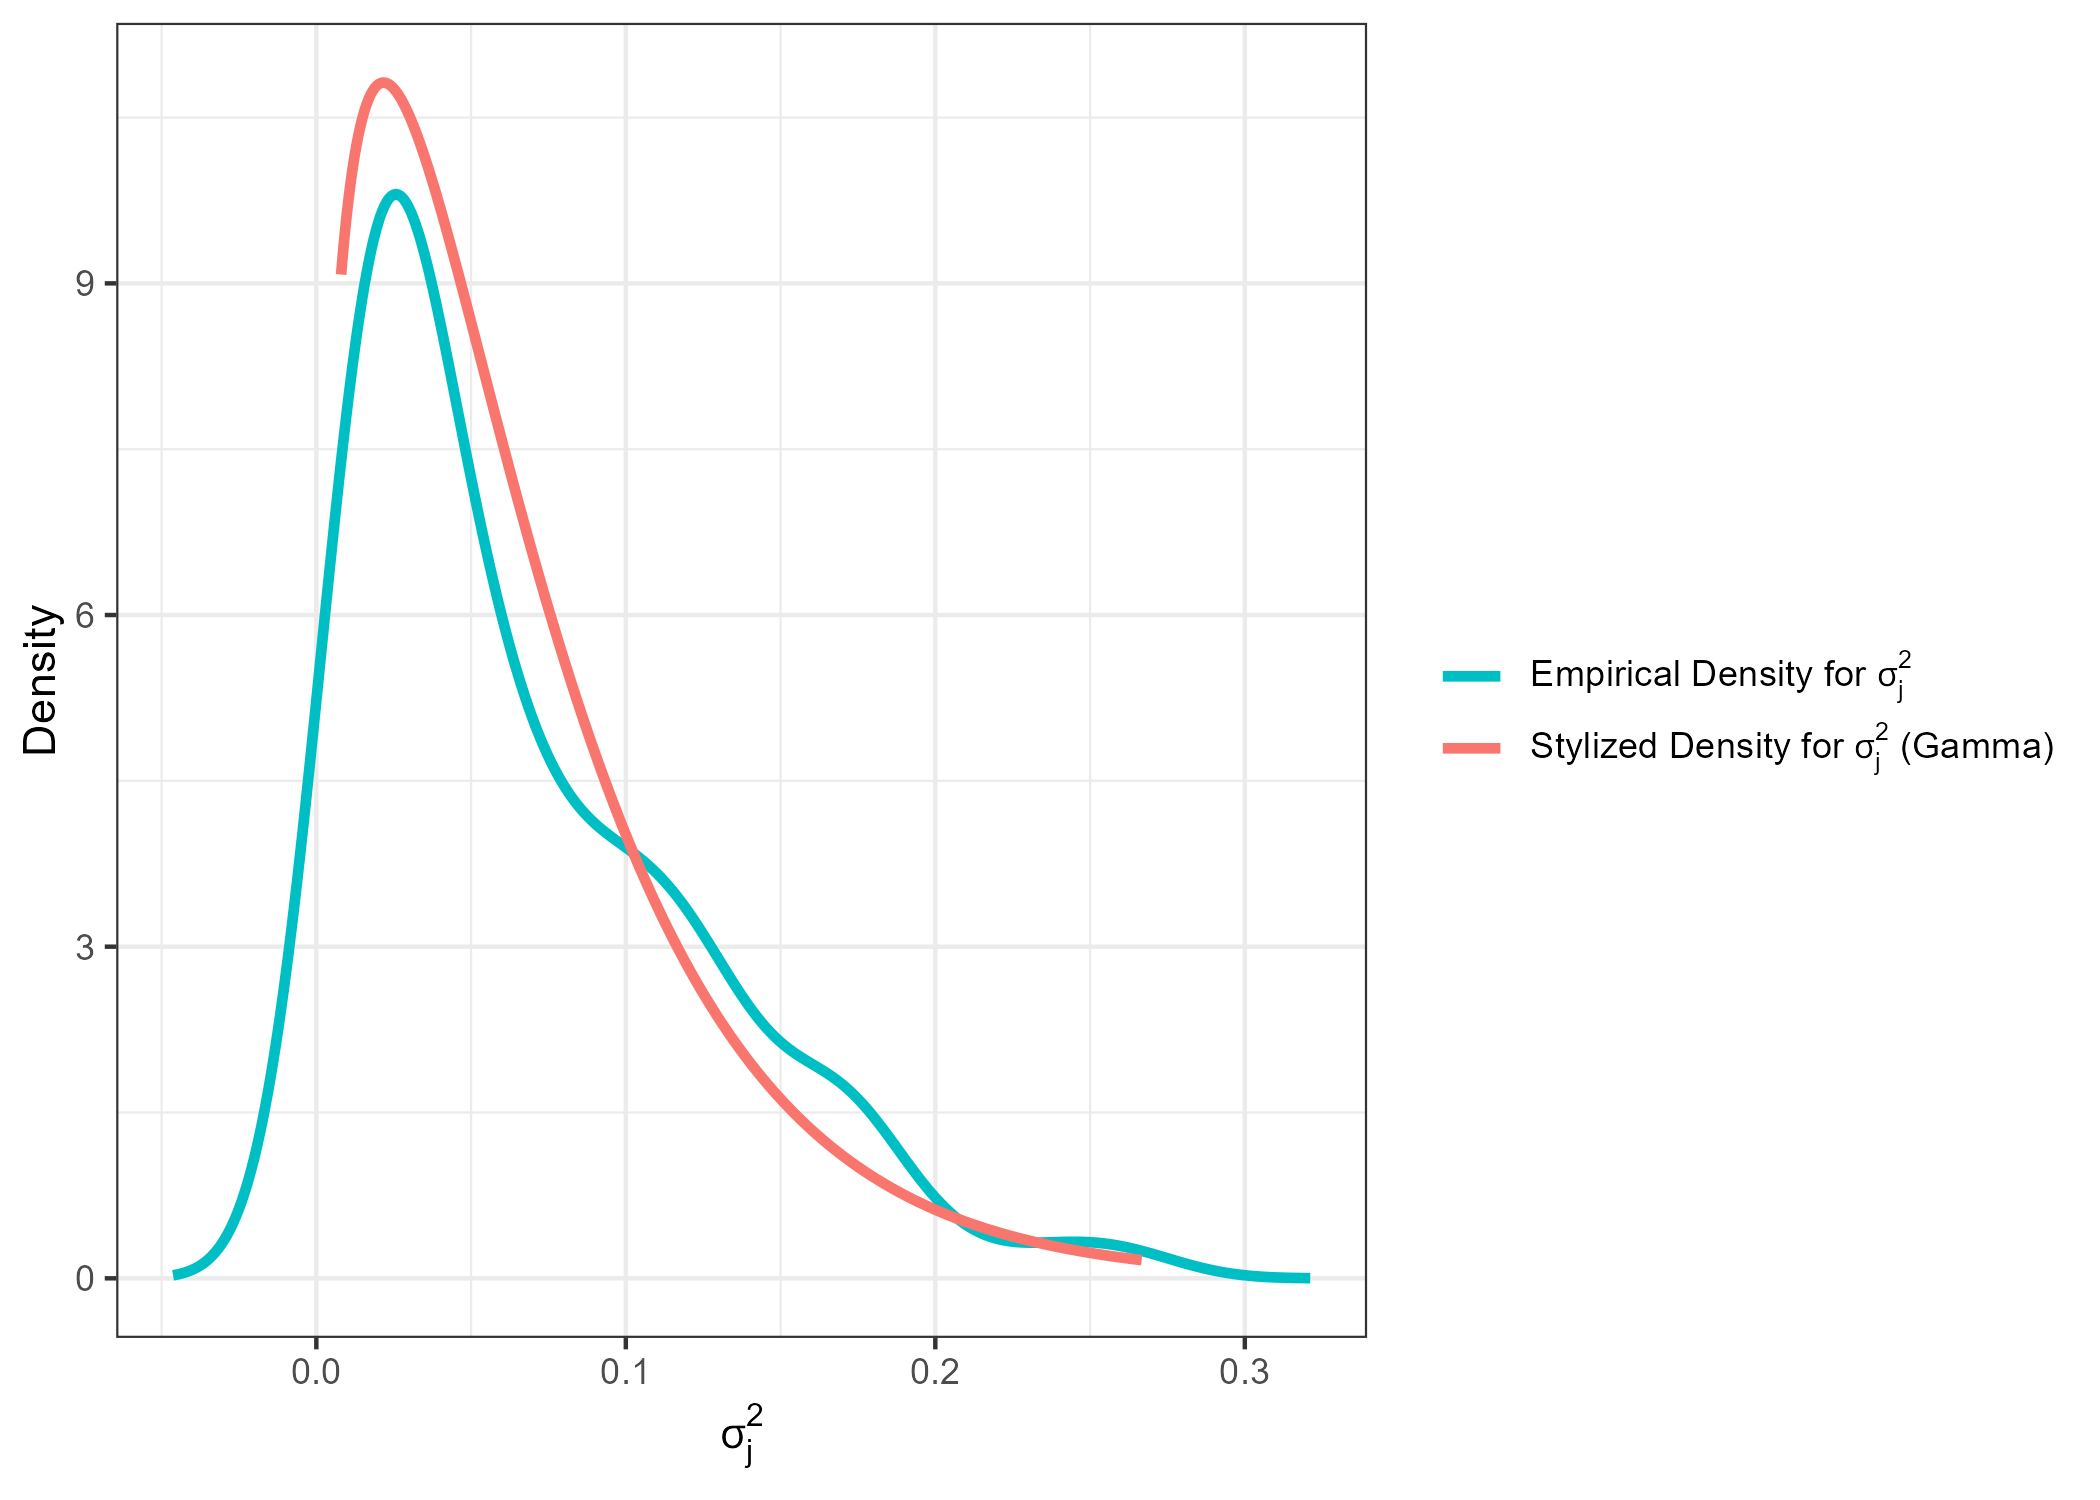
\includegraphics[width=\linewidth]{chapters/plots/densitysigma_j_sq.png}
    \caption{Density plots of $\sigma_j^2$ from Empirical vs Stylized Sampling Methods. \label{fig:densitysigma_sq}}
    \vspace{-5pt}
\end{figure}


\begin{figure}[H]
    \centering
    \vspace{-5pt}
    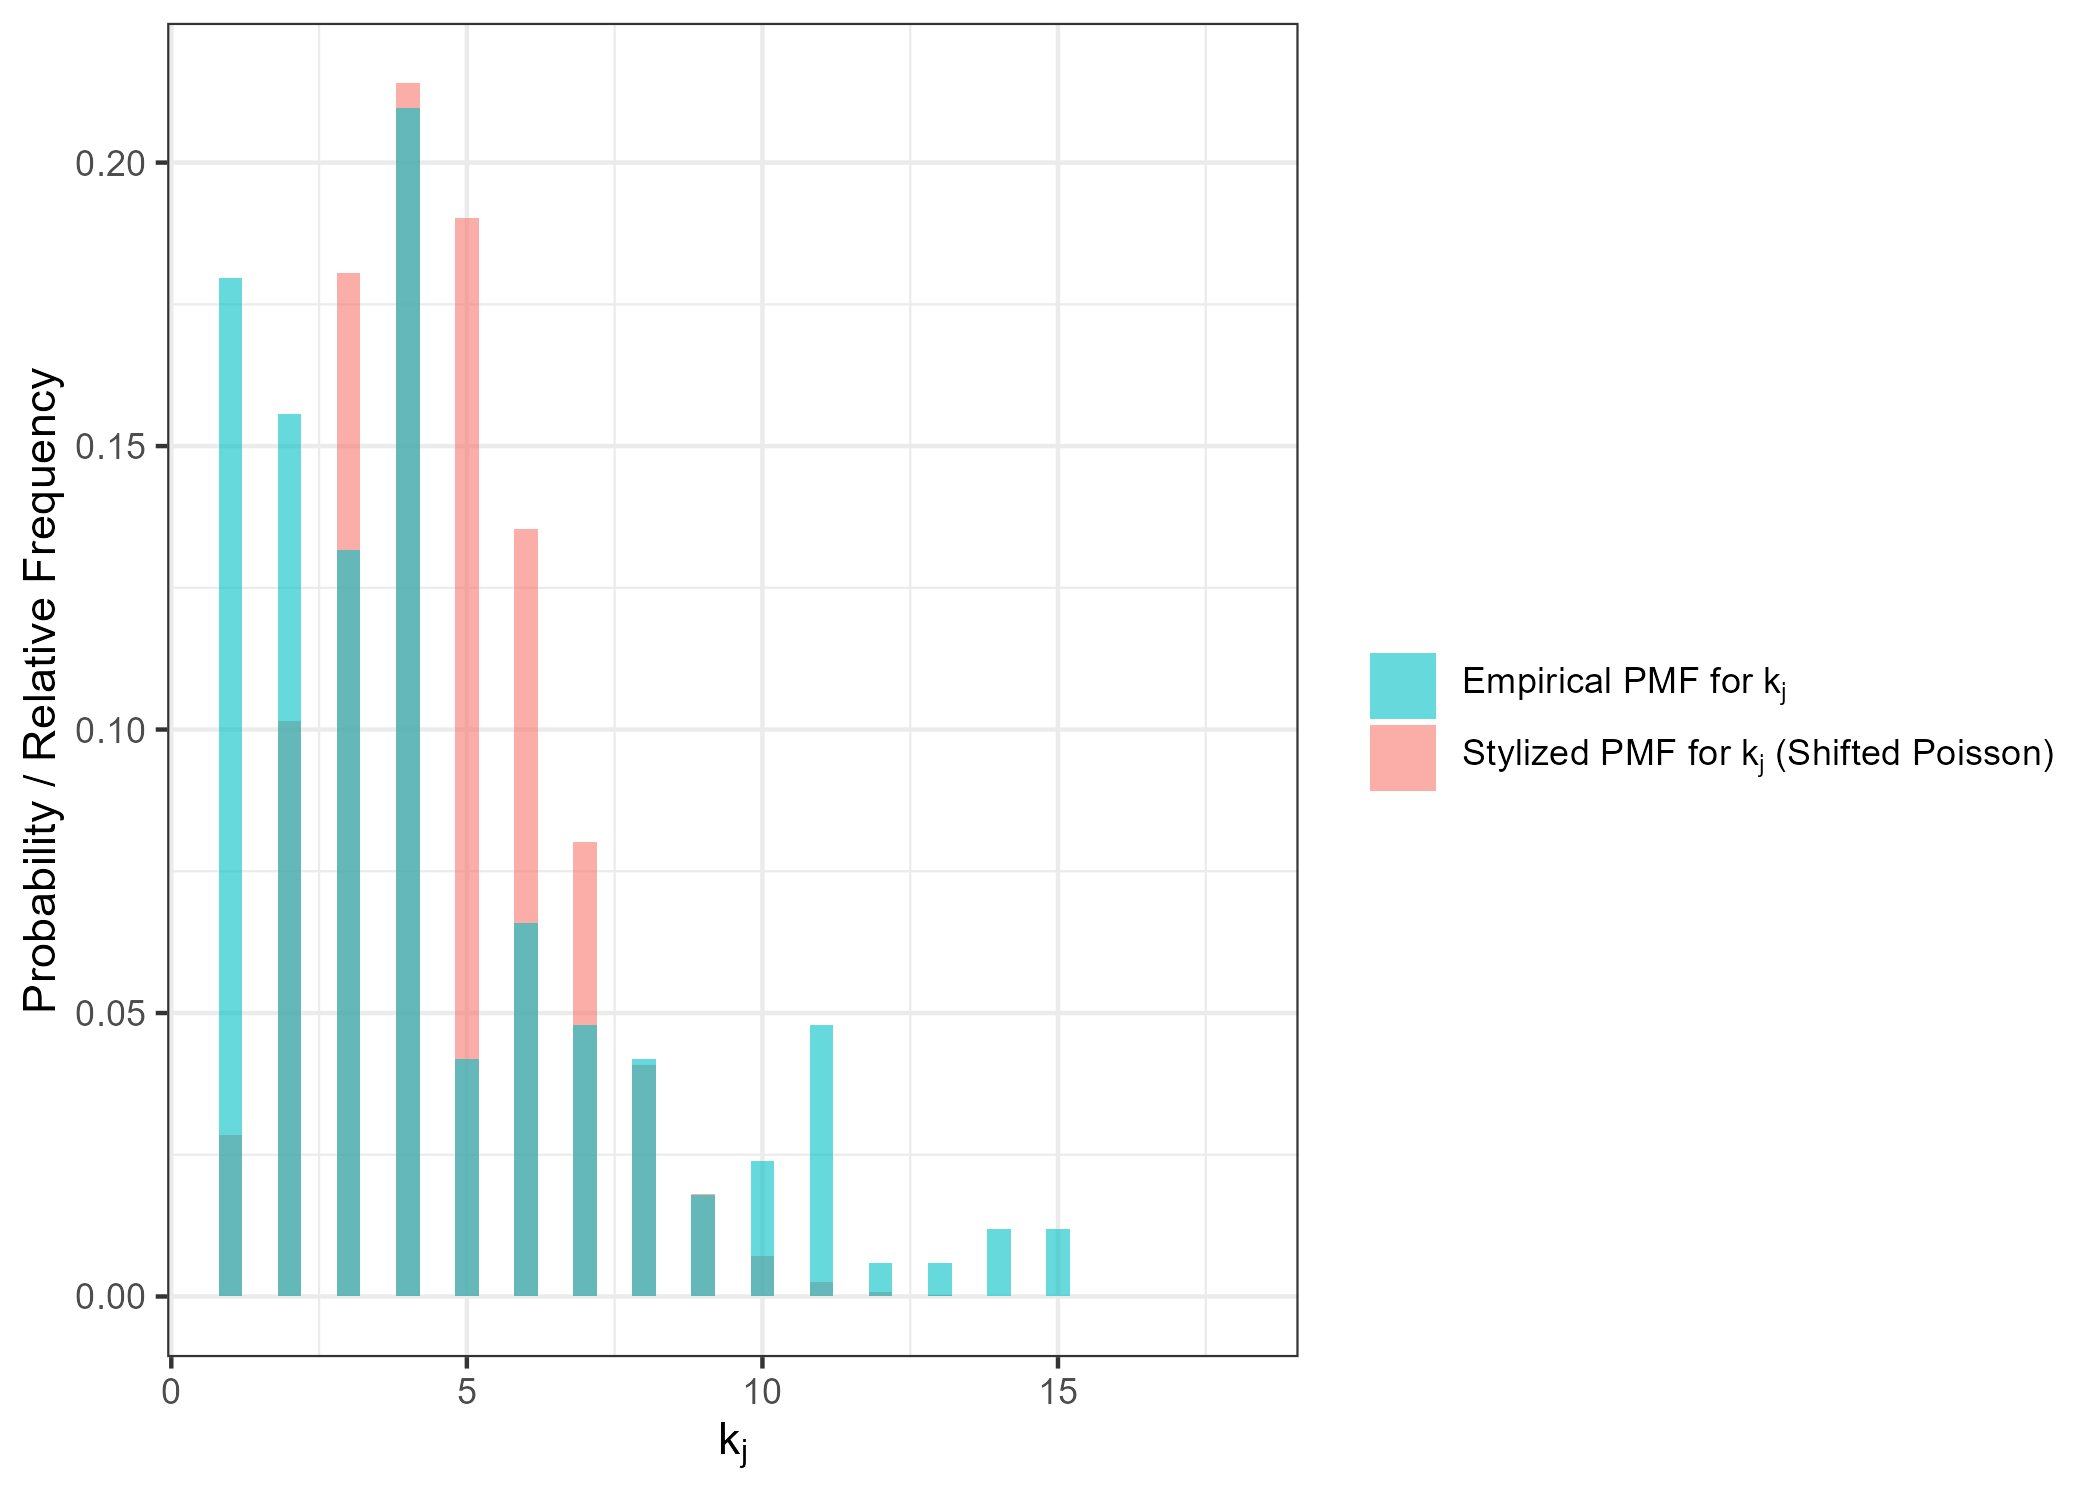
\includegraphics[width=\linewidth]{chapters/plots/pmfkj.png}
    \caption{PMF Plots of $k_j$ from Empirical vs Stylized Sampling Methods. \label{fig:pmfkj}}
    \vspace{-5pt}
\end{figure}

For the third method of obtaining $k_j$ and $\sigma_j^2$, the balanced assumption method, I estimate power assuming perfect balance where all the studies had the arithmetic means for $\sigma_j^2$ and $k_j$ of the empirical dataset from data generation, \textcite{WilliamsRyan2022HiMI}. This is the exact same way that the $\mu_c$ values are generated, so the approximation will return whatever the power neighborhood level, $P$,  is for that condition. Under this sampling method, we can see how different the true simulated power is from the power neighborhood value in that condition. 

\section{Simulation Design}\label{sec:simulationdesgin}

Before settling on the design conditions for the simulation study (see Table \ref{tab:experimentalconditions}), I first evaluated what each combination of parameters implies about the maximum $\mu_c$ values to see if any were unreasonably large. After generating the $\mu_c$ values, I graphed the maximum $\mu_c$ value of each $\bm{\beta}$.

Figure \ref{fig:max_mu} below displays all the generated maximum $\mu_c$ values of a $\bm{\beta}$ vector for the study, broken down by $f_c$, $\tau$, and $J$. There is some variation in the $\mu_c$ values beyond the factors in the Figure due to the $\rho$, $\omega$, and balance of the $j_c$ factors. In this study, the largest possible $\mu_c$ value is 1.43. Based on this exploration of the design conditions, I decided to remove $J=12$ condition because it resulted in a maximum $\mu_c$ value greater than 3 SD, which is not common in educational research \autocite{KraftMatthewA.2020IESo}.  The factors that seemed to have an impact on the magnitude of the $\mu_c$ values were $J$, $f_c$, $P$, the balance of the $j_c$, and $\tau$. The $\rho$ and $\omega$ had less of an impact on the magnitude of the max $\mu_c$ value. 



\begin{sidewaysfigure}
    \centering
    \vspace{-5pt}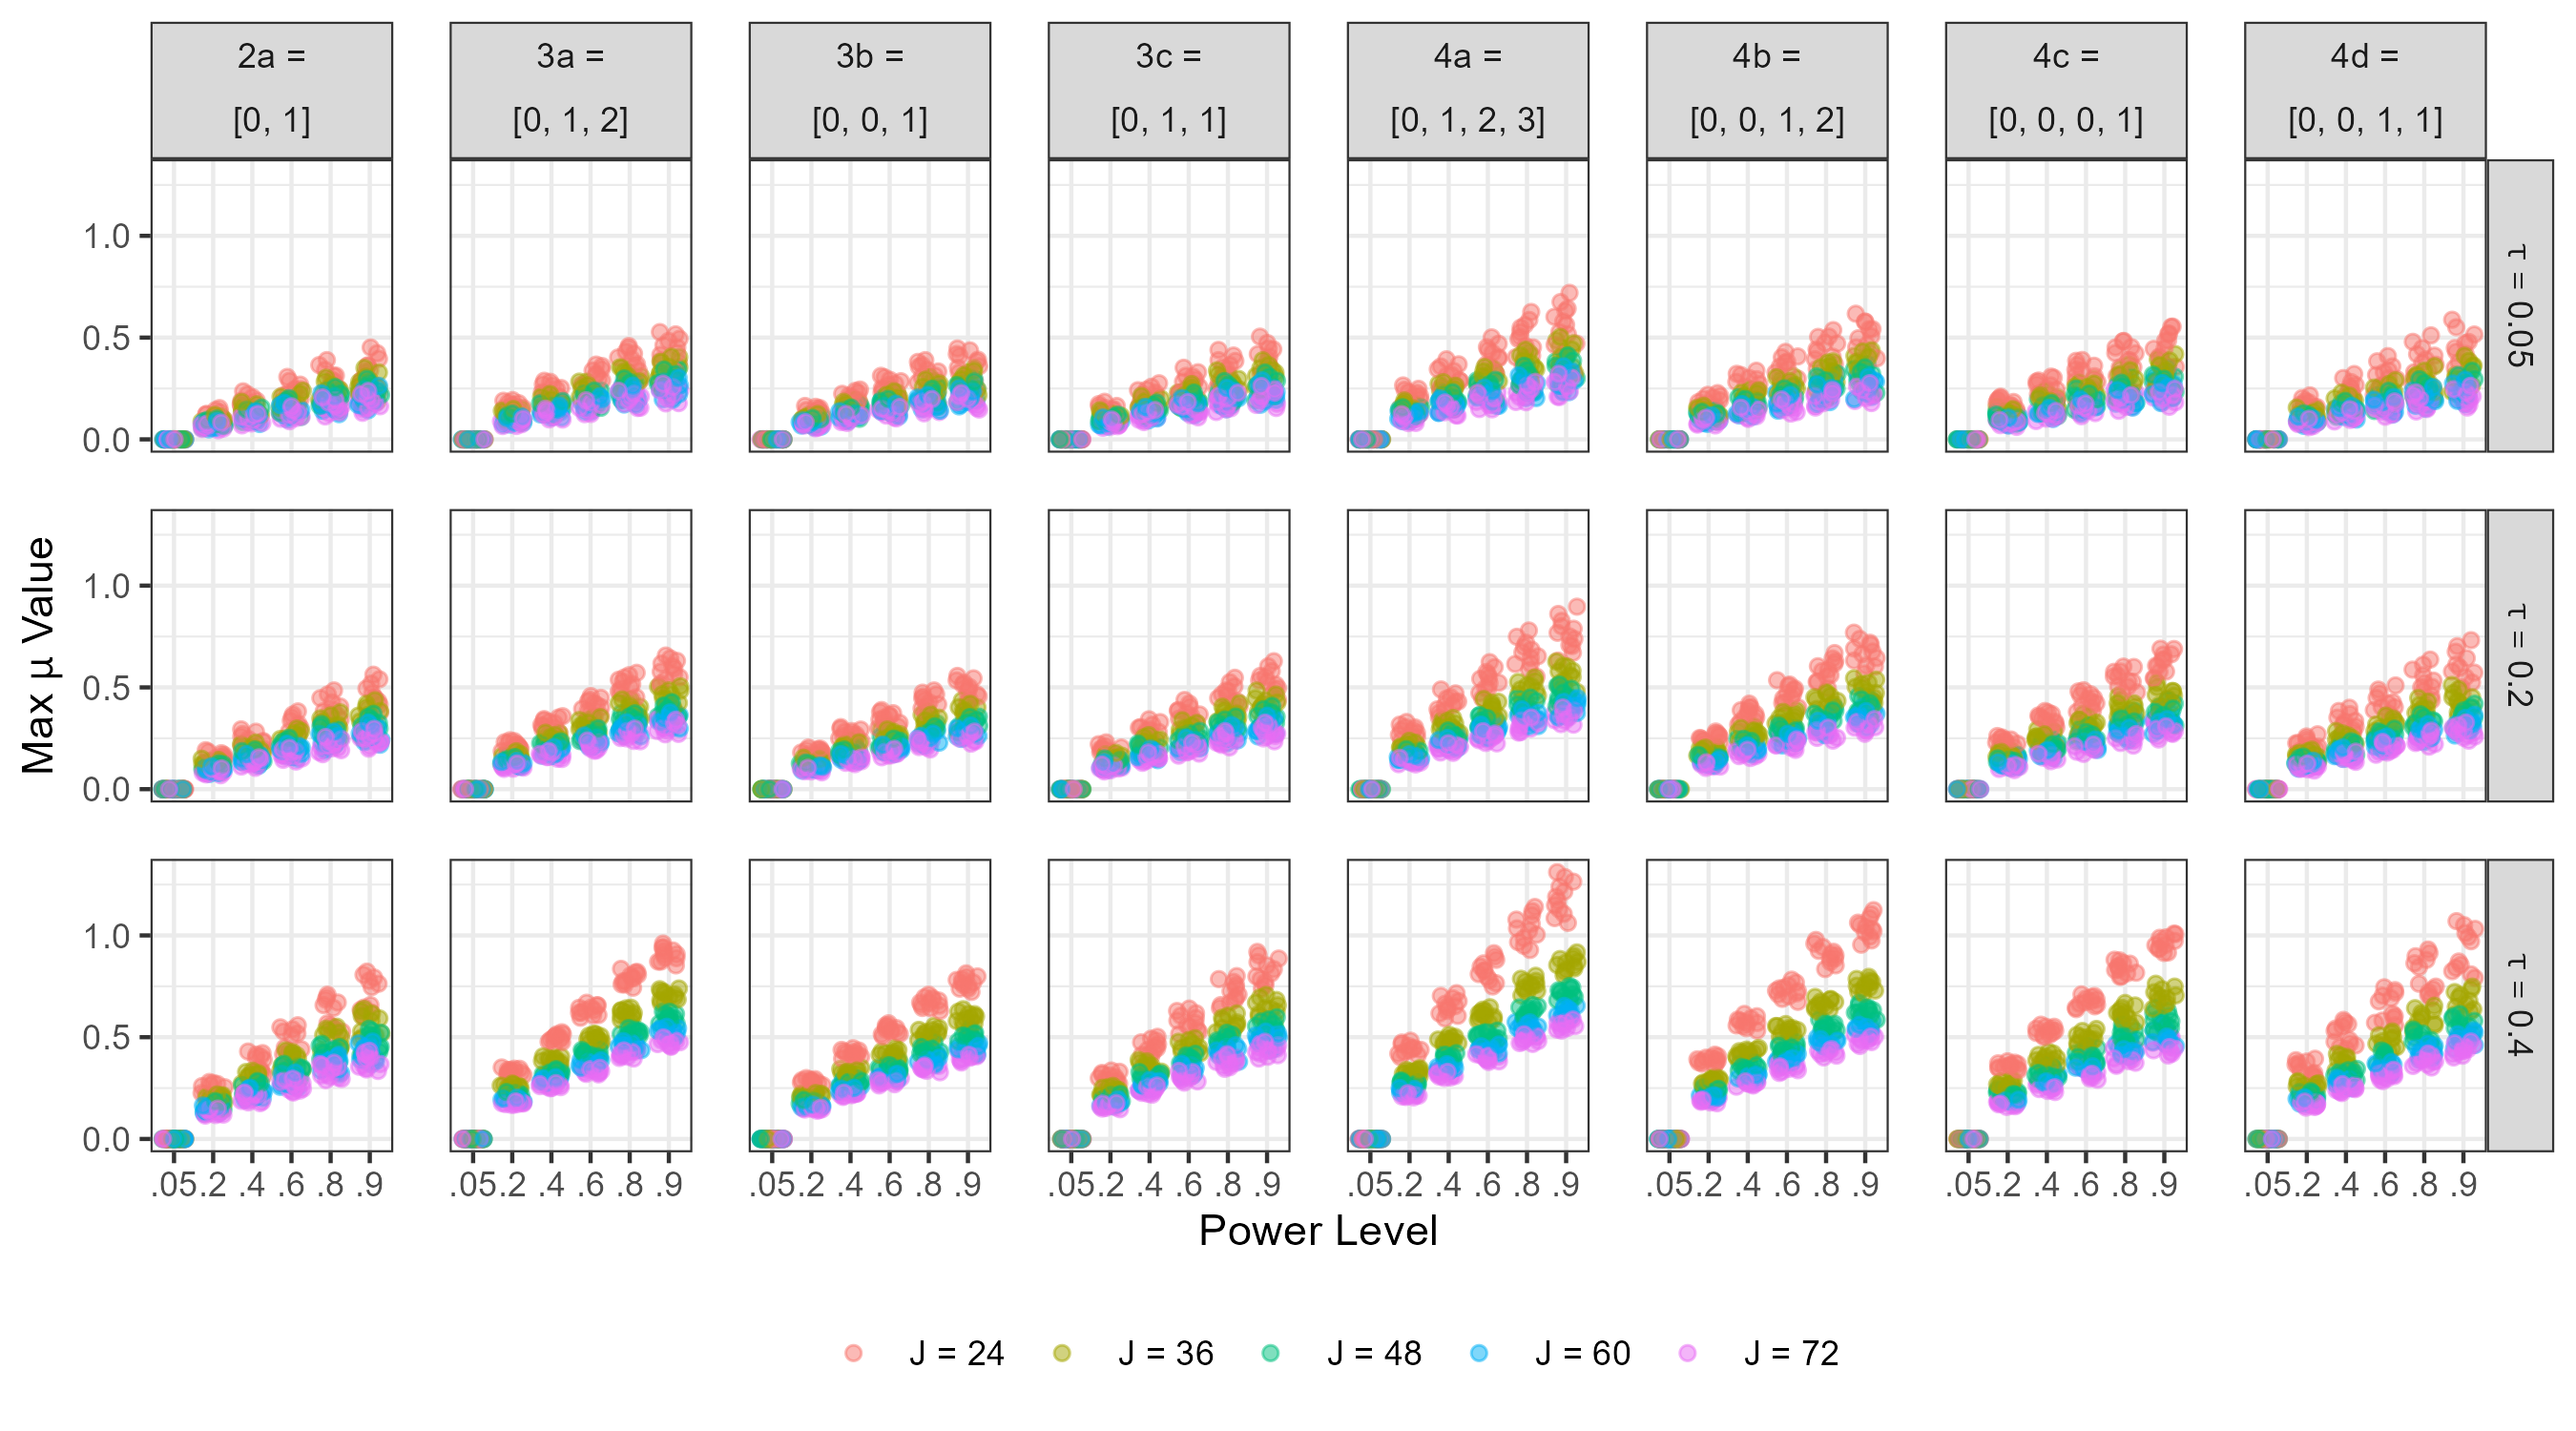
\includegraphics[width=\linewidth]{chapters/plots/max_mu.png}\caption{The max $\mu_c$ value by the pattern type ($f_c$), between-study heterogeneity ($\tau$), and the number of total studies ($J$). \label{fig:max_mu}}
    \vspace{-5pt}
\end{sidewaysfigure}




\subsection{Simulation Design Conditions}\label{sec:simulationdesgin}

In this section, I detail the simulation design conditions. The factors that I examined included: (1) the number of categories ($C$), (2) the total number of studies ($J$), (3) the balance of the number of studies across categories (balanced $j_c$ vs. imbalanced $j_C$), (4) pattern type ($f_c$), (5) between-study heterogeneity ($\tau$), (6) within-study heterogeneity ($\omega$), (7) sampling correlation ($\rho$), and (8) power neighborhood ($P$). Table \ref{tab:experimentalconditions} summarizes the design conditions. In the following sections, I provide more details on each of the factors examined. 


% To validate the approximation, we will find the multiplier needed to give a power level. Given the rest of the meta-analytic data characteristics and the primary study characteristics, if you want to obtain a power level of $40\%$, how big does $\zeta$ need to be? 

\begin{table}[H]
\caption{Simulation Parameters}
     \label{tab:experimentalconditions}
    \centering
    \begin{tabular}{p{7cm}p{7cm}}
        \toprule
    Factor & Value \\ \midrule
       % Number of Categories ($C$) & 2, 3, 4 \\
       % Pattern Type ($f_c$) & AD or 50-50-Bal (8 patterns across $C$) \\

       Pattern Type ($f_c$)  & 2a, 3a, 3b, 3c, 4a, 4b, 4c, 4d \\
       Number of studies ($J$)  & 24, 36, 48, 60, 72  \\ 
       Between-study heterogeneity ($\tau$)  & 0.05, 0.20, 0.40 \\
       Within-study heterogeneity ($\omega$) & 0.05, 0.20 \\
       Sampling correlation ($\rho$) & .2, .5, .8 \\
       Power Neighborhood ($P$) & $5\%$ $20\%$, $40\%$, $60\%$, $80\%$, $90\%$ \\
       Balance of $j_c$ Across Categories & balanced $j_c$ vs imbalanced $j_c$ \\
        \bottomrule
    \end{tabular}
   
    \small
    
   % \caption{Caption}
\end{table}


\subsubsection{Pattern Type ($f_c$)} \label{sec: Pattern Type}
%and Number of Categories ($C$)


Table \ref{tab:patterns} and Section \ref{sec: patterns} detail the patterns of $\mu_c$ for each number of categories condition. For a given pattern, the first $\mu_c$ of each pattern was 0, and the rest of the $\mu_c$ is determined by the value of $\zeta$, which is found with the power neighborhoold condition, study-level weights, $\tilde{w}_{jc}$, and a Type I error set to $\alpha = .05$. 

For the conditions, there are eight patterns across the values of $C$: one when $C = 2$, three when $C = 3$, and four when $C = 4$. They are denoted as:  2a, 3a, 3b, 3c, 4a, 4b, 4c, and 4d.  While there are many other potential values for the $\mu_c$, I choose these patterns because they offer a comprehensive set of $\mu_c$ values to evaluate when validating the power approximation. While the difference between each $\mu_c$ is a whole number times $\zeta$, it is possible to have any portion of $\zeta$ be the difference between categories; I decided only to add a multiple of $\zeta$ as a simplification. Additionally, the reason I set the first $\mu_c$ of each pattern to $0$ is that only the relative distance between $\mu_c$ matters for power. 

%\section{Meta-Meta Methods to Inform Experimental Conditions}
%Regarding the number of $C$ we evaluated, to better understand the characteristics of study-level category moderators, I coded additional information on study-level category moderators from the sample of studies from the meta-analytic dataset of \textcite{tipton2019}. \textcite{tipton2019} reviewed 64 meta-analyses to summarize the meta-analytic methods used in these studies. They coded variables related to the meta-analytic datasets and analyses, such as how many studies, samples, effect sizes, type of design, and the type of moderator analyses. For this dataset, for the meta-analyses that had study-level categorical moderators, I coded and summarized the number of categories.



%For this dataset, for the meta-analyses that had study-level categorical moderators, I coded and summarized the number of categories, number of studies per category, number of effect sizes per category, sample size per category, and magnitude of the overall effect size for each category. The results will inform the values used for my experimental conditions. After coding the additional information from these studies, I may adjust some of the proposed experimental conditions or the datasets used for data generation and validation. 

%Also could refer to these methodological articles for examples of what they did: Pustejovsky and Tipton 2015 2 - 6 Joshi et al. 2023 - for their conditions that use categorical moderators. 


\subsubsection{Number of Studies ($J$) and Balance of the Number of Studies across Categories (Balanced $j_c$ vs. imbalanced $j_c$)}

\paragraph{Number of Studies, $J$}
I examined the following conditions for the number of studies per category: $J = 24, 36, 48, 60, 72$. Because the focus of this study is the power for the Wald test of study-level categorical moderator, and $J$ should have a substantial impact, I decided on a large range of values of $J$ to better evaluate this factor. Also, I chose values that are multiples of 12, because they would divide into integers across the values of $C$ in both levels of the balance of the number of studies per category, $j_c$ (details on this below). 

\paragraph{Balanced $j_c$ vs. imbalanced $j_c$ across $C$} 

For the balance of the $j_c$ condition, I looked at how the number of studies is distributed across the categories through two conditions: 1) balanced $j_c$ and 2) imbalanced $j_c$. The details of this condition are in Section \ref{sec: detailsbal}

The interaction between the distribution of the $\mu_c$ values and the balance of the number of studies across the categories impacts power. I imposed various patterns of the $\mu_c$ intercepts for each of the categories (see Table \ref{tab:patterns}). Each pattern started with a known value of $\mu_1 = 0$, while at least one category had a $\mu_c$ that is greater than 0. By having the category with the largest $\mu_c$ value have the largest number of studies, then there should be more power for the Wald test of multiple categories. Since we are validating the approximation, I decided to make this simplification. While this is not exhaustive for the distribution of balance across a study-level categorical covariate, this setup demonstrates how extreme imbalances in the number of studies across categories and their interaction with the value of the $\beta$ slope impact power. 

The smallest number of studies per category, $j_c$, is $j_c = 4$ when there are imbalance $j_c$, $J = 24$, and the number of categories $C = 4$. The largest number of $j_c$ per category is when 54 studies are in one category, when $J= 72$, there are imbalanced $j_c$, and $C=2$. The extreme range of meta-analyses included in the simulated datasets is necessary to understand how the number of studies factor and the balance of the $j_c$ factor impact the power of a test for a categorical moderator. 

%While a categorical moderator only having $4$ studies is quite small, I have encountered categorical moderators that have that many studies within one category in practice.  


\subsubsection{Between-study Heterogeneity ($\tau$), Within-study Heterogeneity ($\omega$), and Sampling Correlation ($\rho$) }
For the values of between-study heterogeneity ($\tau$), within-study heterogeneity ($\omega$), and sampling correlation ($\rho$), I decided to follow the values used by \textcite{vembye2023}. For the between-study heterogeneity, the authors used $\tau = 0.05$, $0.2$, and $0.4$ to represent a small, medium, or large  $\tau$ value. They chose those values to match those observed across broad literature in social science meta-analyses \autocite{LindenAudreyHelen2021HoRR}. For the within-study heterogeneity, they used $\omega = 0.0$, $0.05$, $0.1$ and $0.20$ to represent no, small, medium, and large $\omega$ values, and that $\omega$ is typically smaller than $\tau$. For the sample correlation values, they evaluated $\rho = 0$ , $.2$, $.5$, $.8$, to represent no, small, moderate, and large $\rho$ values. I looked at the same conditions as well across the parameters, except I decided not to include  $\omega = 0$ and $\rho = 0$ conditions since I aim to validate the power approximation derived for the CHE model on data generated from CHE, while \textcite{vembye2023} also evaluated approximations for the CE and MLMA model for data generated from the CHE model. For my purposes, I chose not to look at special cases of the CHE model where there is no within-study variance or no correlation among effect sizes. To reduce the number of conditions and cut down on computational time, I chose not to include $\omega=0.1$. 

\subsubsection{Power Neighborhood}
For the power neighborhood levels, I decided to cover a large range of values: $5\%$, $20\%$, $40\%$, $60\%$, $80\%$, and $90\%$. The power level of $5\%$ is the Type I error rate because I set an $\alpha = .05$ for the nominal Type I error rate for the entire study. When the power neighborhood value equals the true Type I error rate, NCP was equal to 0, and I assessed the Type I error rate of the test. I decided to do a broad range for the rest of the power levels since I am trying to find NCP and, therefore, $\mu_c$ values from the power levels in combination with the other design factors.

%this is an artifice of this simulation to make sure we cover a range of conditions with respect to power. 


\subsection{Number of Conditions}

There are $8$ patterns across all the values of $C$, so I looked at those in combination. For this simulation study, there are $8$ values for $f_c$, $5$ values for $J$, $3$ values for $\tau$, $2$ values for $\omega$, $3$ values for $\rho$, $6$ values for $P$, and $2$ values for balance of $j_c$, resulting in $8640$ conditions.  


\subsection{Performance Criteria}
For this analysis, the primary performance criterion of interest is the discrepancy between the approximated power estimates and the true simulated power estimates found by the rejection rate for the cluster-robust Wald test using a CHE working model. The discrepancy is measured as the average of the approximated power estimates minus the rejection rates for each condition. Additionally, I am also interested in the nominal error rate of the cluster-robust Wald test when using a CHE working model, which is found when $ P=.05$. Below, I detail how I calculated the rejection rate for the simulated data, the MCSE of the rejection rate, the MCSE for the approximation estimates, and the MCSE for the discrepancy between the power estimates and the true power estimates. 

For the power estimates of the approximation results, $T$, with $K$ number of replications, the MCSE is:

\begin{equation}
    MCSE_{approx} = \sqrt{\frac{S^2_T}{K}}
\end{equation}
where $S_T^2$ is the sample variance, $S_T^2 = \frac{1}{K-1}\sum_{k=1}^K(T_k - \overline{T})^2$. 

I generated 150 power estimates using the approximation for each condition. I came up with 150 power estimates per condition by running some tests within one condition and calculating the MCSE. From these tests, I determined that I needed about 150 power estimates per condition to have MCSE values $\leq 0.01$. Then, I averaged the power estimates up to the condition level, resulting in $8640$ average power estimates.

For the simulated data, I calculated the rejection rate for the cluster-robust Wald test, which is the proportion of replications where a test returned a p-value less than the criterion $\alpha$-level: $\rho_{\alpha} = Pr(p_r < \alpha)$, where $R$ is the number of simulation iterations, $p_r$ is the p-value from replication $r$, $r = 1, \cdots, R$. The rejection rate is estimated as:
\begin{equation}
    r_{\alpha} = \frac{1}{R} \sum_{r=1}^R I(p_r < \alpha).
\end{equation}
The corresponding Monte Carlo standard error for the rejection rate estimate is (Morris et al., 2019):
\begin{equation}
    MCSE_{r_{\alpha}} = \sqrt{r_{\alpha}(1-r_{\alpha})/R}.
\end{equation}
I used $\alpha = .05$ for the rejection rate across all conditions. I compared the empirical rejection rate to the approximation results in each condition.

I generated 2,500 replications for each combination of conditions. By running 2,500 replications, the $MCSE < 0.01$ for every condition since with $r_{\alpha} = 0.5$, then $\sqrt{\frac{0.5(1-0.5)}{2500}} = 0.01$ (Please note, across all values of $r_{\alpha}$,  $ MCSE_{r_{\alpha}}$ is highest when $r_{\alpha} = 0.5$ ). 


Finally, because the approximated power and simulated power are independent, the MCSE of the discrepancy between the approximated power result and the true (simulated) power result is the following:

\begin{equation}
    \sqrt{MCSE_{r_{\alpha}}^2 + MCSE_{approx}^2}.
\end{equation}


\subsection{Analysis of Deviance for Power Discrepancies} \label{sec: analysis of deviance}

Following the methods of \textcite{vembye2023}, I ran a generalized linear model (GLM) on the power discrepancies for the empirical sampling method. I first transformed the approximation power results from probabilities to quantiles to be used in the "probit" link function (the cumulative standard normal distribution function), since this function converts probabilities to z-scores. Also, since the data is binomial (probability of rejection), the weights are set to the number of trials, which in this case is the number of iterations.  

Then, the transformed approximation power results are included in the formula as an offset term. Essentially, the model subtracts the offset z-score from the observed outcome z-score and then fits the linear predictors to that difference by including the offset (residual z-score).

In addition to this model, I also ran a GLM model on the rejection rates when $P=.05$ to test the nominal error. This model also used a "probit" link function, but did not include the offset term for the approximation power estimates, so the outcome was only the probability of rejection. 

Both models include the main effect for each factor and all the two-way interactions between factors. The only difference is that the model for the nominal error did not include the power neighborhood factor, $P$.  

I summarized the influence of each factor using an analysis of deviance, which I used to determine which factors to focus on when constructing the figures. I reported the deviance, which is the reduction in twice the log-likelihood for each term, where a higher deviance means more variation is explained in the outcome by that term. I did not assess the magnitude of each deviance, but I ranked all the deviances from largest to smallest and looked at the top 10 factors to get an idea of which factors were the most salient. 


\subsection{Details on Reproducibility}

All analyses were run on the University of Texas's Stampede3 supercomputer provided by the Texas Advanced Computing Center (TACC) (Skylake Compute Nodes; \url{https://docs.tacc.utexas.edu/hpc/stampede3/}). The code for this study can be found on \url{https://github.com/bethanyhamilton/PowerMeta_StudyCatMod}. Furthermore, for total replicability, I created Docker containers for the study. The Docker container allows you to completely control variables that may impact the results, like R or package versions, script versions, or even operating system differences in C-level linear algebra libraries. The simulation study is located here: \url{https://hub.docker.com/r/bethanyhamilton/powstudcatmod/tags}, and the approximation study is located here: \url{https://hub.docker.com/r/bethanyhamilton/powstudcatmod_approx/tags}. For this study, I used R \autocite[version 4.4.2;][]{R} with Linux kernel (version 5.15.153.1-microsoft-standard-WSL2). Linear algebra computations used LAPACK \autocite[version 3.12.0;][]{lapack99}. For the approximation study, I used the following R packages:
\texttt{mvtnorm}  \autocite[version 1.3-3;][]{mvtnorm}, \texttt{stringr}  \autocite[version 1.5.1;][]{stringr}, \texttt{purrr} \autocite[version 1.0.41;][]{purrr}, \texttt{dplyr} \autocite[version 1.1.4;][]{dplyr}, and \texttt{tidyr} \autocite[version 1.3.1;][]{tidyr}. In addition to these packages, for the simulation study, I also used \texttt{clubSandwich} \autocite[version 0.5.11;][]{pustejovsky2024a}  and \texttt{metafor} \autocite[version 4.8-0;][]{viechtbauer2010a}.


%\section{Implications} 
%summarize the expected contribution

%The results of this study will validate the power approximation for the tests of study-level category moderators in meta-regression of dependent effects. The results of my study can be directly applicable to applied meta-analysts who wish to conduct an a priori power analysis for their prospective meta-analytic study. Furthermore, this study will give more guidance on the performance and limitations the CHE+RVE model when it comes to the true power of the tests of study-level category moderators. 
%possible limitations ** 
%-these results can also be applied to Fisher-Z transformed correlation effect sizes. Still, the results will not translate to other effect size types like odds ratio without further assumptions \autocite{vembye2023}.

%Mention that we will not do pairwise comparisons. We have not yet done that --so I  need to find the joint distribution of the test statistics. 
\chapter{Results}\label{ch: results}

In this chapter, I present the convergence rates for the CHE+RVE model used to obtain the rejection rates of the simulation study. Then, I present the MCSE for the approximation power estimates, the MCSE of the rejection rates, and the MCSE of the discrepancy between the two. Finally, I present the results of the Monte Carlo simulation study to obtain the true power and nominal error of the cluster-robust Wald statistics for a study-level categorical moderator using a CHE working model and the results of the approximation to the power of this test.  

\section{Convergence}

Across the factors that I evaluated in the simulation study, the CHE+RVE model with REML estimation had very high convergence rates with a range of (0.9984, 1) across the 8,640 conditions. Only 174 out of 8,640 conditions had some samples that did not converge, and only 259 out of 21,565,440 samples did not converge. The maximum number of samples that did not converge for a condition was 4, so to ensure that I have the same number of samples across conditions, I retained 2,496 samples per condition. 

\section{Monte Carlo Standard Error}

I ran 150 iterations for the approximation results and averaged the resulting power values for each sampling/imputation method per condition. For the empirical sampling method, the range of MCSE values was $(0, 0.011)$ across conditions. For the stylized sampling method, the range of MCSE values was $(0, 0.011)$ across conditions. For the simulated results, I ran 2,496 iterations per condition; this resulted in a range of MCSE values of $(0, 0.010)$. The MCSE of the power difference for the empirical sampling method resulted in a range of MCSE of ($.002,  0.015)$. The MCSE of the power difference for the stylized sampling method resulted in a range of MCSE values of $(0.002, 0.014)$.

For the balanced assumption method results, there is no variation in the approximated power estimates, because it returns the value of the power neighborhood factor as discussed in Chapter \ref{ch: methods}. Therefore, there is no corresponding MCSE estimate for the approximation results, and the MCSE of the discrepancy between the approximation results using the balanced assumption method and the simulated power will be the same as the MCSE of the simulated power. 

\section{Power Discrepancies}

In the following sections, I present the results from the analysis of deviance and visual analysis for the power discrepancies when using the empirical sampling method. Then, I compare the results of the power discrepancies across sampling/imputation methods through a visual analysis.   

\subsection{Analysis of Deviance for Power Discrepancies when using the Empirical Sampling Method} \label{sec: analysis of deviance - empirical}

Table \ref{tab:SequentialAnalysis} below presents the results of the analysis of deviance for power discrepancies of the empirical sampling method (please refer to Section \ref{sec: analysis of deviance} for the methods of this analysis). The primary goal of this analysis is to determine which factors are most salient in explaining the variation of the discrepancies between the approximation and the true power. As seen in the top row of this table, the residual deviance from the null model was 48808.6. The deviance reported in the subsequent rows is the reduction in twice the log-likelihood of each corresponding term, and they were calculated sequentially in order from top to bottom. I also added a column for the ranking of the deviance from largest to smallest. From this table, the following are the top ten factors and interactions based on the ranking of the deviance: 1) the total number of studies ($J$), 2) the pattern of the $\mu_c$ ($f_c$), 3) the interaction between the total number of studies and the pattern of the $\mu_c$  ($J \times f_c$), 4) the interaction between the total number of studies and the balance of the number of studies across categories ($J \times bal. j_c$), 5) the balance of the number of studies across categories ($bal. j_c$), 6) the interaction between the pattern of the $\mu_c$ and the balance of the number of studies across categories ($f_c \times bal. j_c$), 7) the interaction between the power neighborhood and the balance of the number of studies across categories ($P \times bal. j_c$), 8) the interaction between the between-study heterogeneity and the power neighborhood ($\tau \times P$), 9) the interaction between the power neighborhood and the pattern of the $\mu_c$ ($P \times f_c$), and 10) the interaction between the total number of studies and the power neighborhood  ($J \times P$). 

From the results of this analysis, I decided to primarily focus on the pattern of the $\mu_c$ factor, the total number of studies factor, the balance of the number of studies across categories factor, and their interactions when constructing figures, because they explained the majority of the variation in the power discrepancies. I also decided to examine the between-study heterogeneity factor in conjunction with the other factors to see its impact after accounting for the other factors. To evaluate the effect of the power neighborhood, $P$, I include the levels as tick marks on the x-axis in the figures in the next section. As a consequence, to see the impact of the power neighborhood, you can evaluate the trajectory of the magnitude of the discrepancies as you move along the x-axis. These results also suggest that the within-study heterogeneity factor and the sampling correlation factor had little impact on the discrepancies between the power estimates from the approximation and the true simulated power when using the empirical sampling method for the approximation. 

\begin{table}[H]
\caption{Sequential Analysis of Deviance for Power Discrepancies when using the Empirical Sampling Method}
     \label{tab:SequentialAnalysis}
    \centering
    \begin{tabular}{p{3cm}p{3cm}p{3cm}p{3cm}}
        \toprule
    Term & d.f. & Deviance & Rank \\ \midrule
       Null deviance & & 48808.6 & \\
        &&&\\
       $Deviance$ & & & \\
       $J$ & 4 & 8369.0 & 1 \\
       $\tau$ & 2 & 357.3 & 14  \\ 
       $\omega$ & 1 & 6.0 & 24 \\
       $\rho$ & 2 & 18.5 & 19 \\
       $P$ & 5 & 499.2 & 13 \\
       $f_c$ & 7 & 7130.3 & 2 \\
       $bal. j_c$ & 1 & 1823.3 & 5 \\
       $J:\tau$ & 8 & 646.7 & 11  \\ 
       $J:\omega$ & 4 & 9.6 & 22 \\
       $J:\rho$ & 8 & 20.6 & 18 \\
       $J:P$ & 20 & 932.5 & 10 \\
       $J:f_c$ & 28 & 4998.6 & 3 \\
       $J:bal. j_c$ & 4 & 1852.4 & 4 \\
       $\tau:\omega$ & 2 & 12.8 & 21 \\
       $\tau:\rho$ & 4 & 38.9 & 16 \\
       $\tau:P$ & 10 & 1081.8 & 8 \\
       $\tau:f_c$ & 14 & 546.2 & 12 \\
       $\tau:bal. j_c$ & 2 & 133.8 & 15 \\
       $\omega:\rho$ & 2 & 0.2 & 27 \\
       $\omega:P$ & 5 & 30.4 & 17 \\
       $\omega:f_c$ & 7 & 4.8 & 25 \\
       $\omega:bal. j_c$ & 1 & 0.0 & 28 \\
       $\rho:P$ & 10 & 6.5 & 23 \\
       $\rho:f_c$ & 14 & 13.4 & 20 \\
       $\rho:bal. j_c$ & 2 & 1.9 & 26 \\ 
       $P:f_c$ & 35 & 1080.9 & 9 \\
       $P:bal. j_c$ & 5 & 1245.6 & 7 \\
       $f_c:bal. j_c$ & 7 & 1505.0 & 6 \\
        \bottomrule
    \end{tabular}
   
    \small
      d.f. = Degrees of freedom; $J$ is the total number of primary studies factor; $\tau$ is the between-study heterogeneity factor; $\omega$ is the within-study factor; $\rho$ is the sample correlation factor; $P$ is the power neighborhood factor; $f_c$ is the pattern of the $\mu_c$ factor; $bal. j_c$ is the balance of the $j_c$ factor. 
   % \caption{Caption}
\end{table}


\subsection{Approximation Performance for the Empirical Sampling Method}

To determine if the power approximation accurately estimated the power of the Wald test of a study-level category model using the CHE+RVE model, I examined the discrepancy between the power estimate of the approximation when using the empirical sampling method and the rejection rates of the simulated data. I primarily focus on the empirical sampling method to obtain $k_j$ and $\sigma_j^2$. This is the best-case scenario for the approximation to result in accurate power estimation, because I use the same empirical distributions to generate my simulated data as did \textcite{vembye2023}. Under this sampling method, I can evaluate how the data-generating factors influence the accuracy of the approximation. Based on empirical study characteristics, I found that the power approximation is generally within five percentage points of the true power, except when the number of categories was four, the total number of studies was small, and the number of studies per category was imbalanced across the categories. Furthermore, the magnitude of the between-study heterogeneity amplifies the degree to which the power approximation overestimates the power under those conditions, where the smallest $\tau$ value ($\tau = 0.05$) resulted in the greatest discrepancies. 

Figures \ref{fig: fc_J_bal_empirical}, \ref{fig: fc_J_bal_empirical_bal_all}, \ref{fig: df_mean}, and \ref{fig: fc_rho_omega_empirical} display the results of the approximation performance for the empirical sampling method for obtaining $k_j$ and $\sigma_j^2$ used in the approximation. In all these figures, the y-axis represents the difference between the approximated and true (simulated) power. The solid lines represent no difference between the approximation and the simulated data. The dashed line at $-0.05$ denotes the threshold for the approximation underestimating the true power by a magnitude of $5$ percentage points, and the dashed line at $0.05$ is the threshold for the approximation overestimating the true power by a magnitude of $5$ percentage points. 

Figure \ref{fig: fc_J_bal_empirical} displays the results of the power discrepancies with the approximated power as the x-axis, the pattern type ($f_c$) and total number of studies ($J$) as facets, and the color of the points mapped to the balance of the $j_c$. This figure shows that the accuracy of the power approximation under the empirical data assumption is impacted by the number of total studies, $J$, the number of categories, $C$, and the balance of $j_c$. Across most of the conditions, the approximation is fairly accurate, where it never underestimates the power, and only a few conditions where it substantially overestimates the power (by as much as 20.81 percentage points); the approximation overestimates true power when there are imbalanced $j_c$, the number of total studies is small ($J = 24$ or $J = 36$), and there are four categories. 

There are minimal discrepancies in power when the number of studies per category is balanced across the levels of the other factors. For the samples that had balanced $j_c$, the approximation overestimates power by at most 7.8 percentage points when $ C=4$. Furthermore, when the total number of studies in a meta-analytic dataset is moderate or larger ($J \geq 48$), then we also see minimal discrepancies, where only a few imbalanced $j_c$ samples resulted in a discrepancy greater than five percentage points when $J = 48$. Finally, when the number of categories is less than four, the power approximation using the empirical distribution rarely overestimates the true power by more than five percentage points. For the $C < 4$, there are only two samples with imbalanced $j_c$, pattern 3b, $J=24$, and $\tau = 0.05$, where it overestimates the power by at most six percentage points.

% For the imbalanced $j_c$ condition when $C = 4$, the smaller proportion of total studies assigned to a category is $\frac{1}{6}$, so that would mean that smallest $j_c$ for the $\mu_c$ vector would be $4$, $6$, or $8$ for $J=24$, $J=36$, or $J=48$, respectively. For $C = 4$, the balanced $j_c$ and $J=24$, it would result in six studies per category, $j_c = 6$, and the imbalanced $j_c$ condition would result in the following $j_c$ values: $j_1 = 4$, $j_2 = 4$, $j_3 = 4$, and $j_4 = 12$.  
%When $C = 3$, the $j_c$ is $j_1 = 6$, $j_2 = 6$, $j_3 = 12$, and the highest $\mu$ value always has $j_3$ number of studies. For the $J = 24$ condition and 

Regarding the different patterns ($f_c$) beyond the number of categories, there is some variation in the magnitude of the discrepancies, with patterns 4c and 3b resulting in the biggest discrepancies within their respective level of $C$. Both of these patterns have one $\mu_c$ value that is different, but the rest have a $\mu_c$ value of 0. However, beyond this pattern type and the number of categories, pattern type was not a particularly notable factor in the accuracy of the approximation.  

\begin{sidewaysfigure}
    \centering\vspace{-5pt}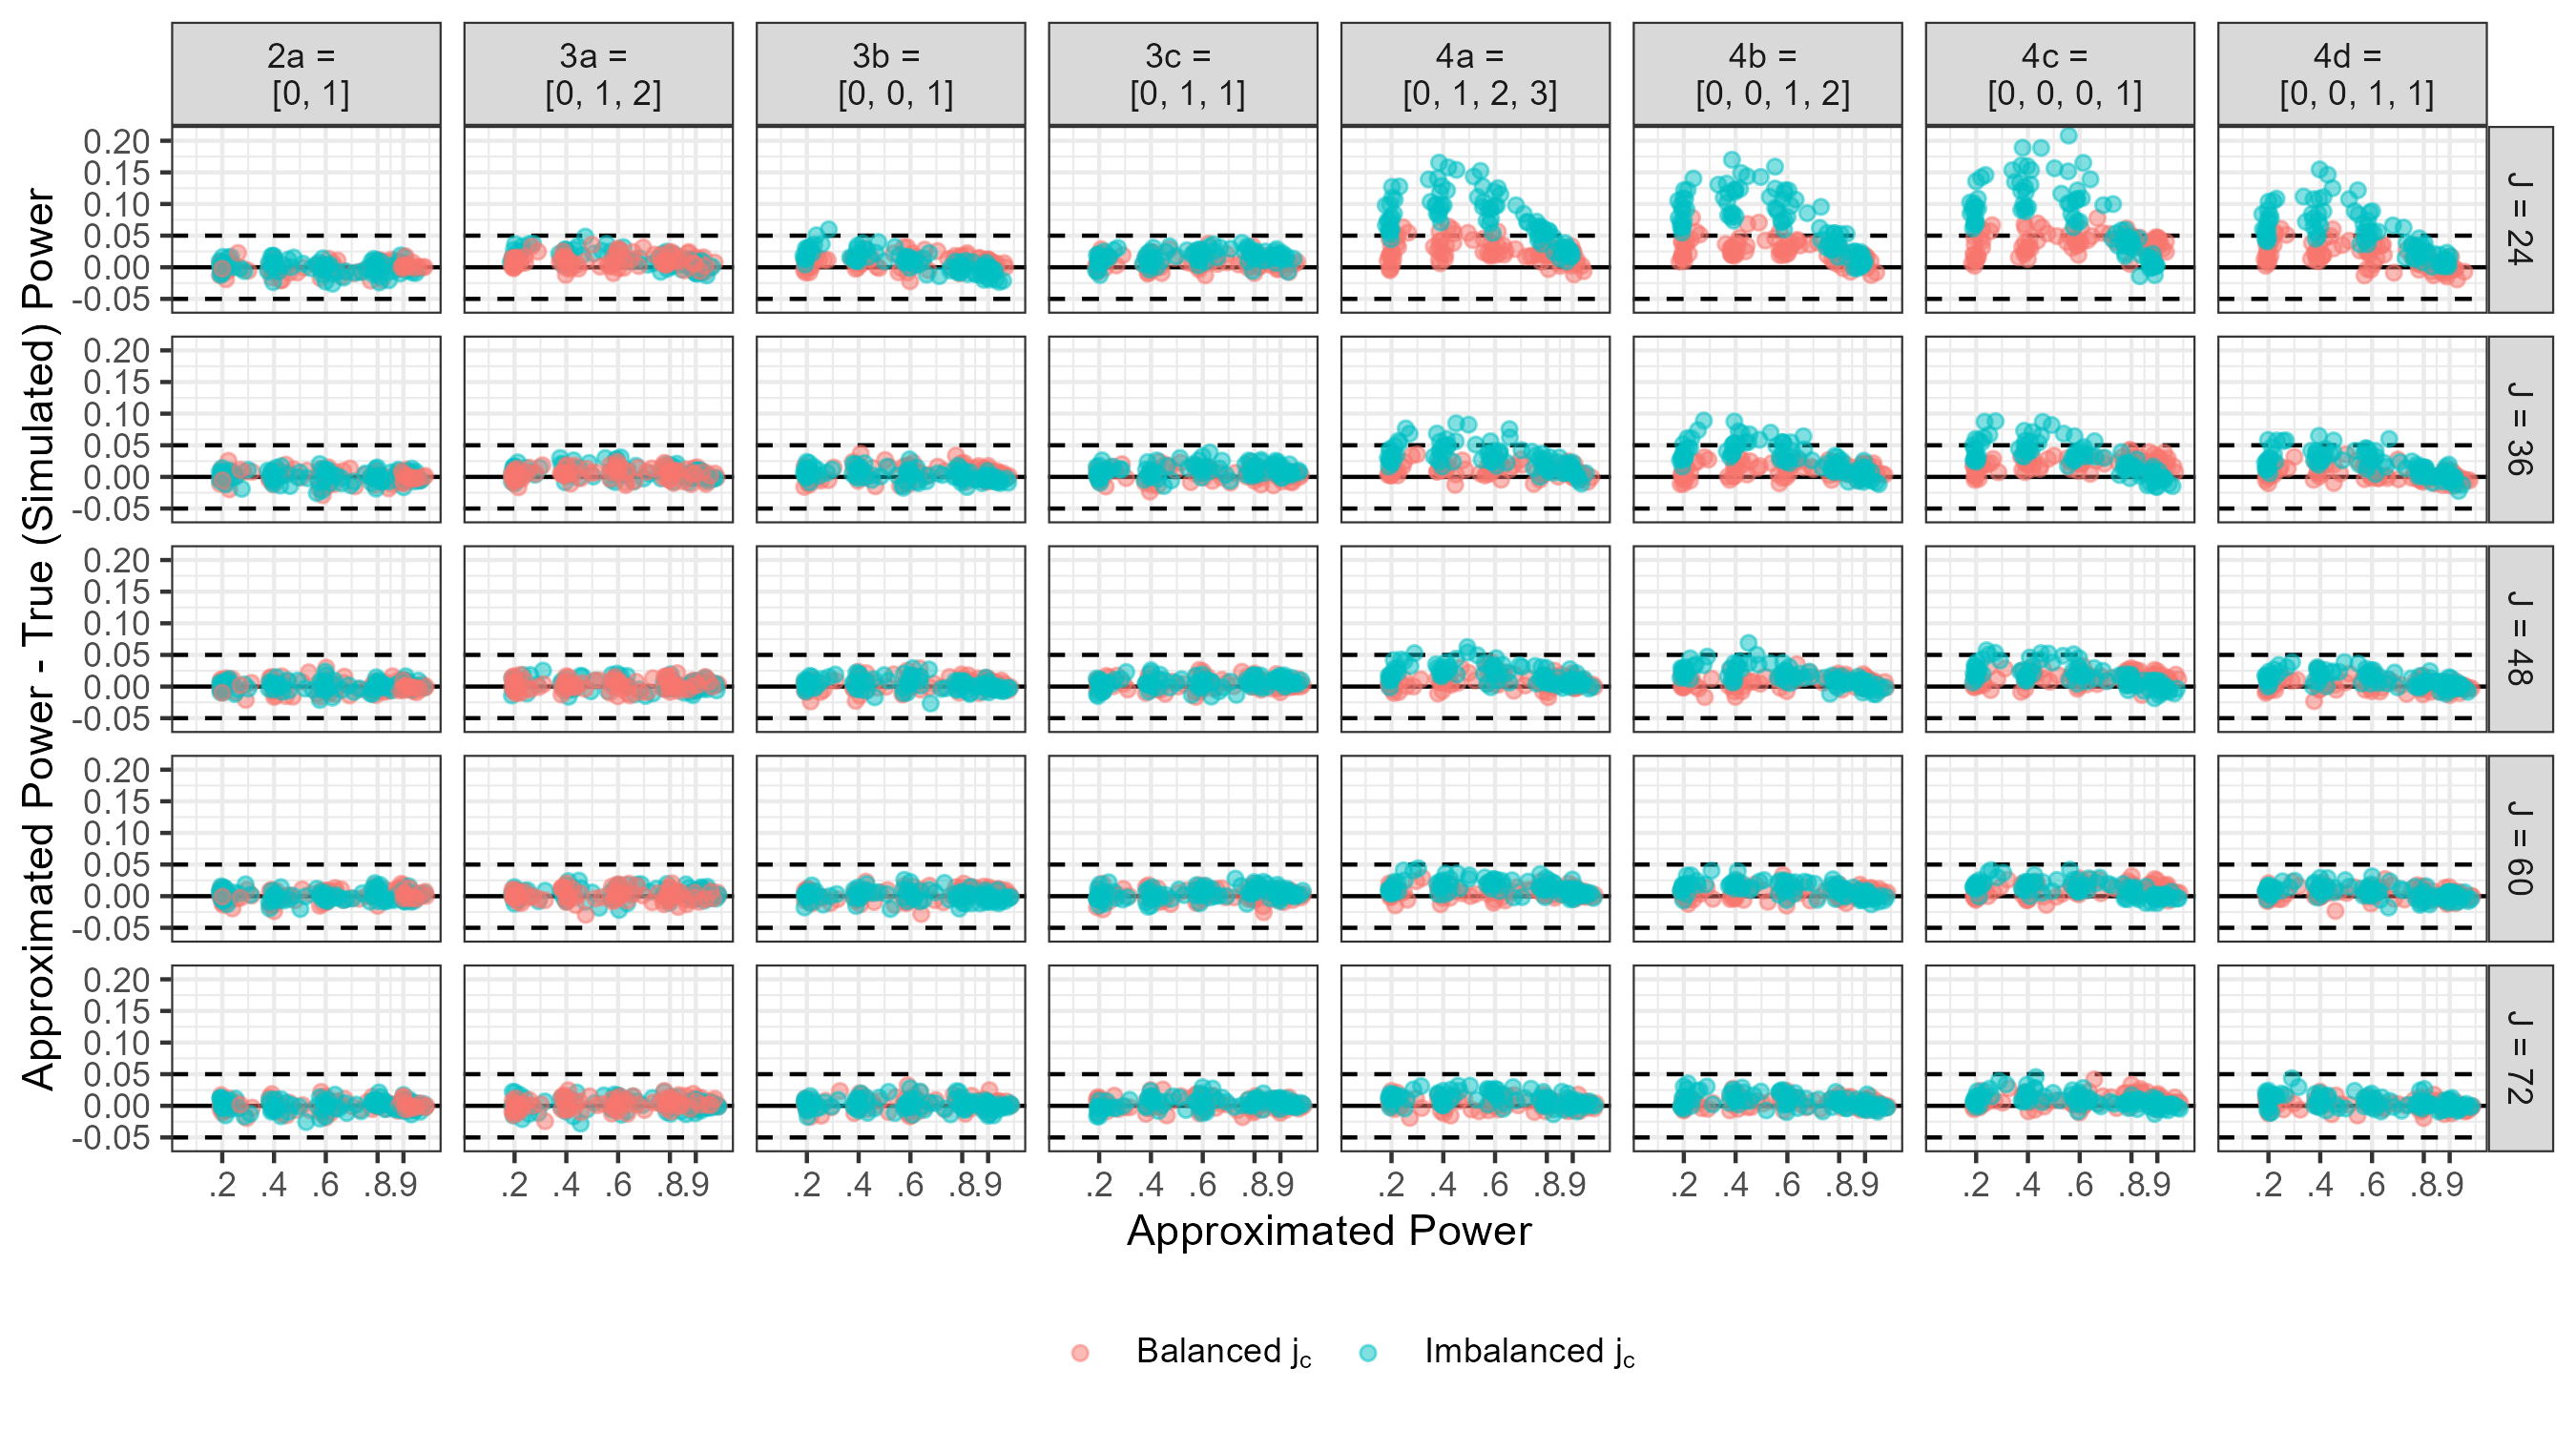
\includegraphics[width=\linewidth]{chapters/plots/fc_J_bal_empirical.png}\caption{Power discrepancy between approximation power and true power vs. approximated power by pattern type ($f_c$), between-study heterogeneity ($\tau$), and the balance of number of studies per category (Balanced $j_c$ vs. Imbalanced $j_c$). The solid lines indicate no discrepancy between the approximated and simulated power. The dashed lines indicate that the approximated power over- or underestimated the true power by five percentage points.\label{fig: fc_J_bal_empirical}}
    \vspace{-5pt}
\end{sidewaysfigure}

To examine the interaction between study heterogeneity, $\tau$, and the power neighborhood, $P$, I created Figure \ref{fig: fc_J_bal_empirical_bal_all}.  Figure \ref{fig: fc_J_bal_empirical_bal_all} displays a graph of the discrepancies for balanced $j_c$, Graph A, and a graph for imbalanced $j_c$, Graph B. Both graphs have the $f_c$ levels where $C = 4$ and when $J$ is equal to $24$ or $36$ as facets, and between-study heterogeneity is mapped to the color. The results show that when the number of total studies is $J = 24$ or $J = 36$ and the number of categories is $C = 4$, then the scale of between-study heterogeneity $\tau$ has a small impact on the magnitude of the discrepancy. The condition where $\tau=0.05$ resulted in the biggest discrepancies in power, especially for samples that had imbalanced $j_c$ (Graph B). Also, the magnitude of $\tau$ does change depending on the value of $P$, where the magnitude of the discrepancies becomes smaller when $P$ is larger. This could be due to range restriction, though. 

\begin{sidewaysfigure}
    \centering
    \vspace{-5pt}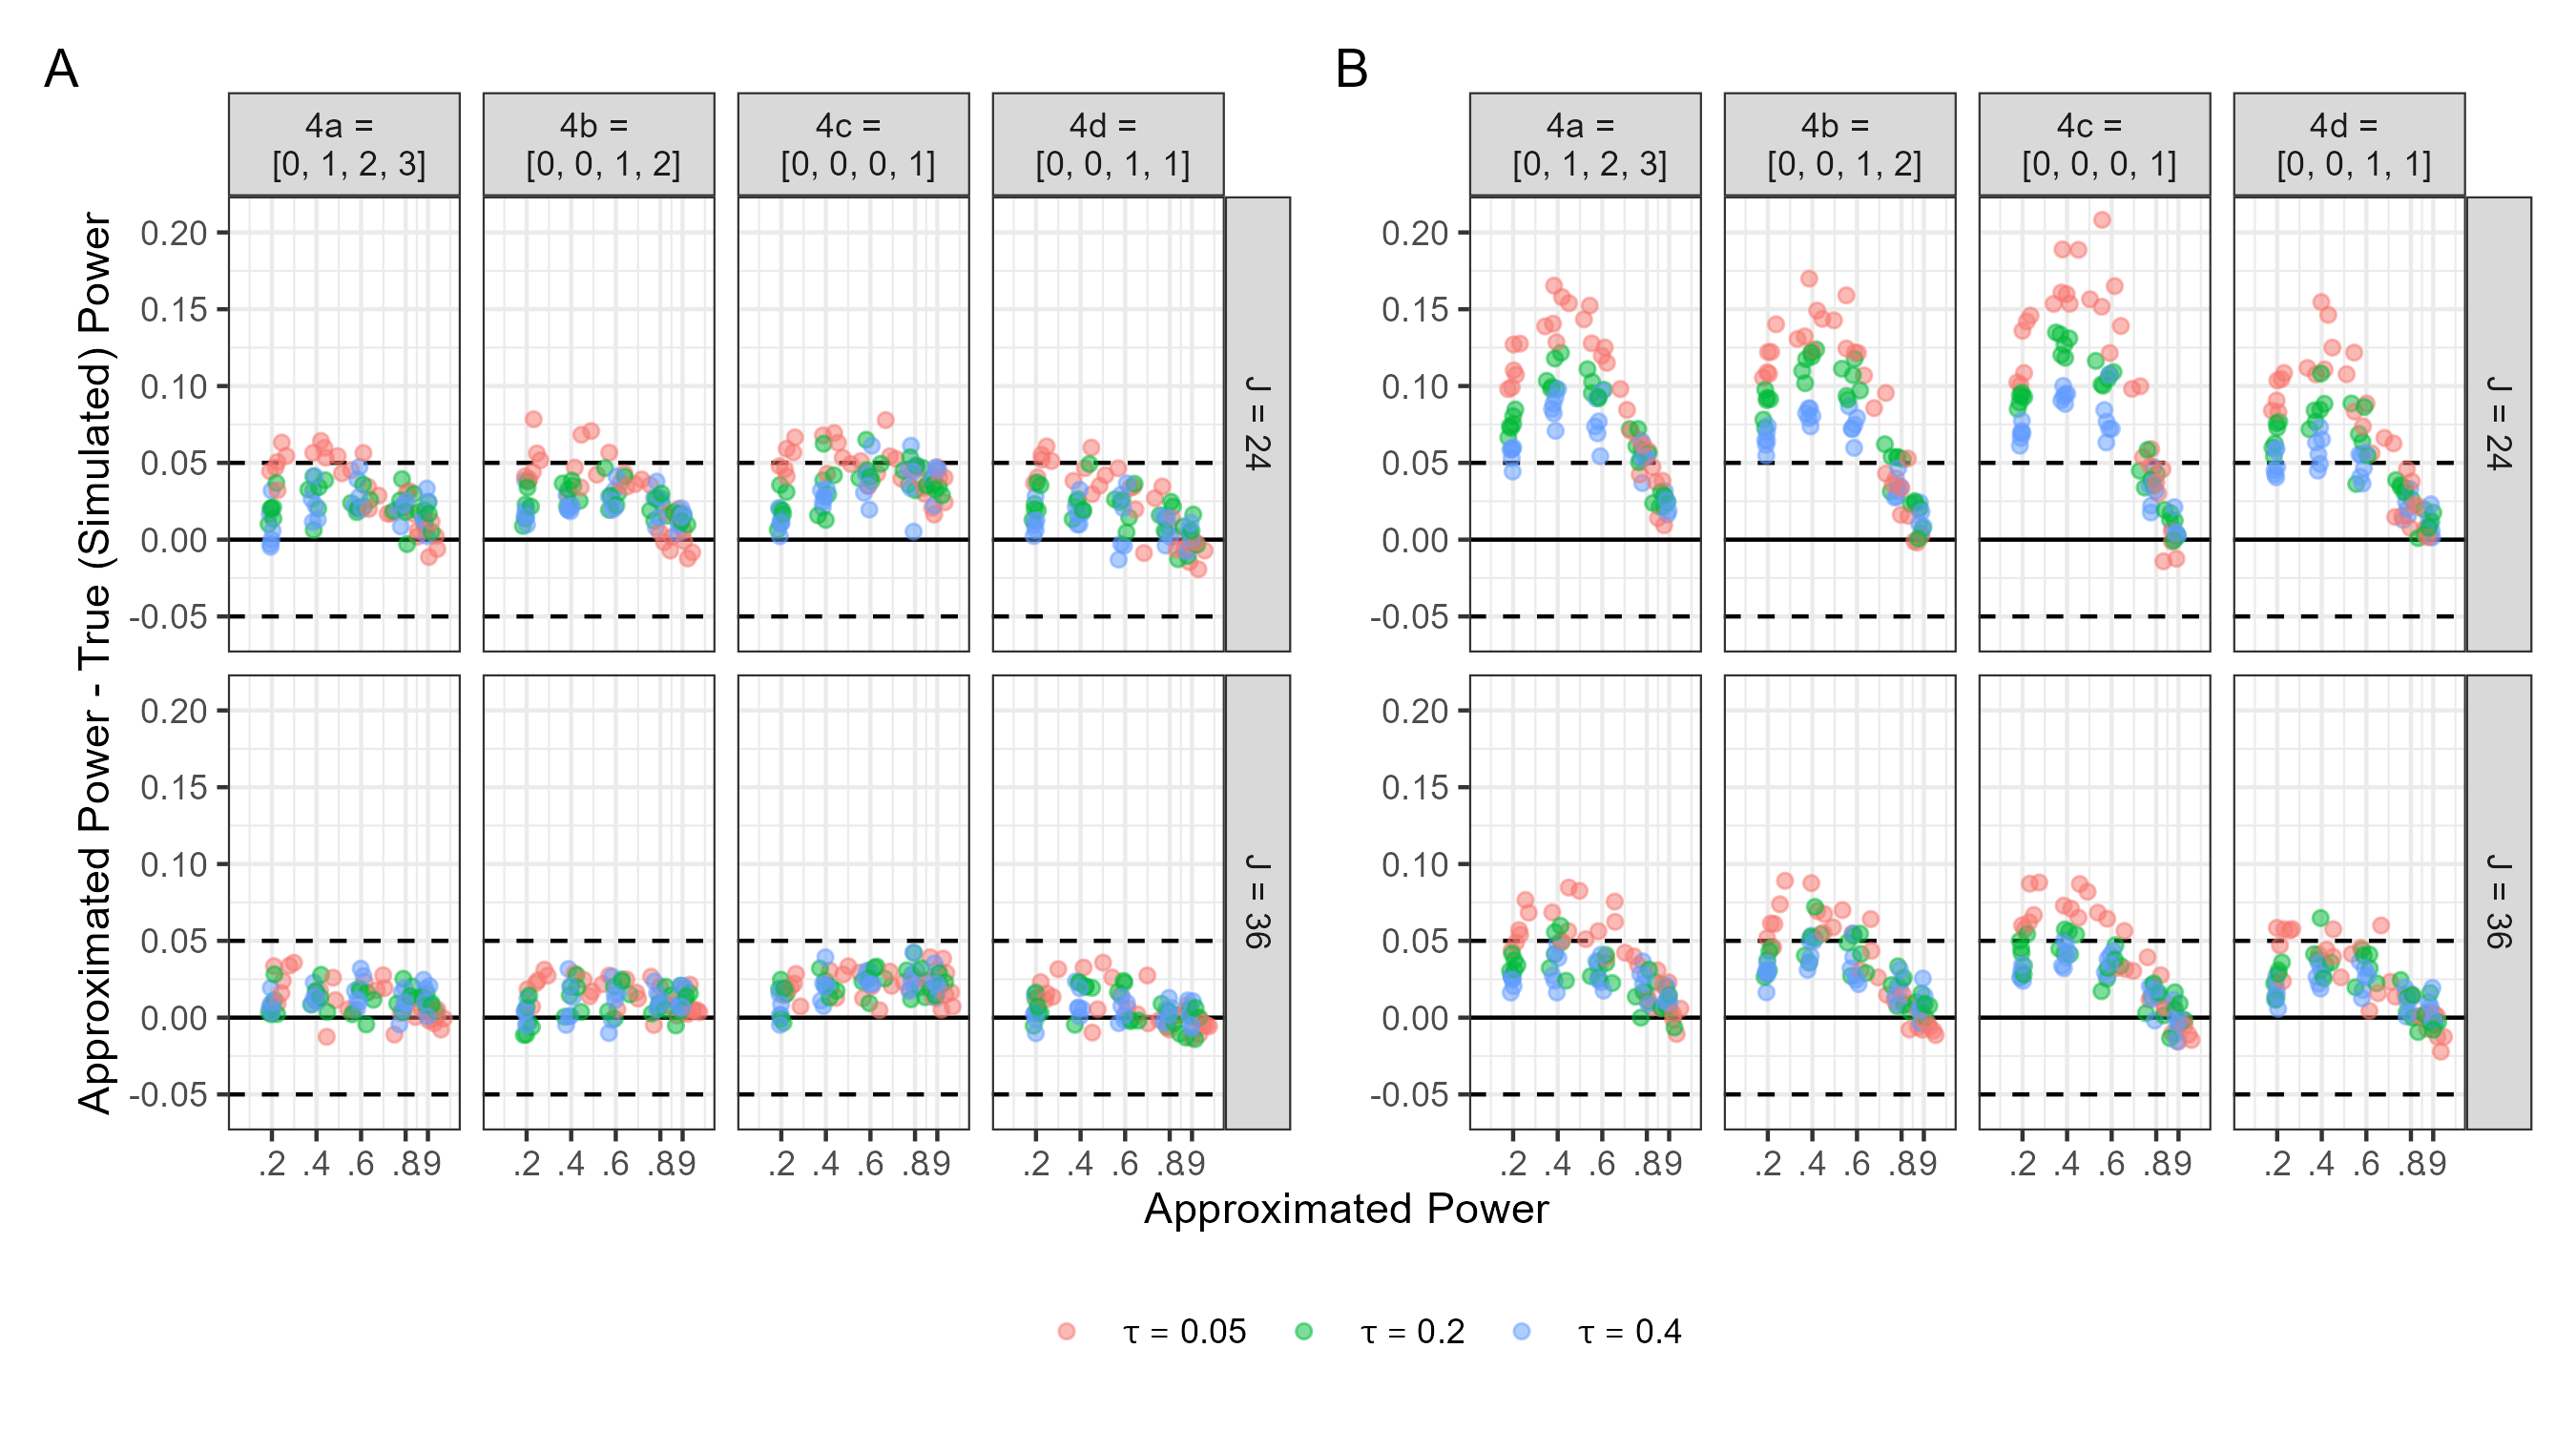
\includegraphics[width=\linewidth]{chapters/plots/fc_J_bal_empirical_bal_all.png}\caption{Power discrepancy between approximation power and true power vs. approximated power by pattern type ($f_c$), the number of studies ($J$), and between-study heterogeneity ($\tau$). Graph A includes only samples with balanced $j_c$, and Graph B includes only samples with imbalanced $j_c$. The solid lines indicate no discrepancy between the approximated and simulated power. The dashed lines indicate that the approximated power over- or underestimated the true power by five percentage points.\label{fig: fc_J_bal_empirical_bal_all}}
    \vspace{-5pt}
\end{sidewaysfigure}

% focus on when the approximation does well

I wanted to see the impact of the study-level weights on the approximation, because more variable study-level weights result in smaller degrees of freedom of the denominator ($d_2$). Therefore, I decided to examine the accuracy of the approximation in relation to the magnitude of the $d_2$. Below is Figure \ref{fig: df_mean}, which has the power discrepancy on the y-axis, the $d_2$ resulting from the approximation formula on the x-axis, the pattern type ($f_c$) as a facet, and the balance of the $j_c$ mapped to color. The figure shows that small values of $d_2$ in combination with the number of categories result in discrepancies of more than five percentage points. The range of $d_2$ values that resulted in power estimate discrepancies of more than five percentage points is $(3.51, 11.64)$, and almost all have four categories (except for the two samples I mentioned earlier from pattern 3b). 

To look at the relationship between the number of studies, $d_2$, the balance of the $j_c$, and the pattern type, I created Figure  \ref{fig:dfvJ}. The figure is a box plot with the number of studies on the x-axis, $d_2$ resulting from the approximation formula on the y-axis, the pattern type ($f_c$) mapped to the column facet, and the balance of the $j_c$ mapped to color. The dashed line marks the maximum $d_2$ value that resulted in a power discrepancy greater than five percentage points ($d_2 = 11.64$). This figure shows that the balance of the $j_c$ impacts the magnitude of the $d_2$ and that the value of $d_2$ cannot be used as a diagnostic alone. While all of the power discrepancies greater than five percentage points had smaller $d_2$, it is necessary to consider the number of categories because there are many samples in patterns 2a, 3a, 3b, and 3c that have $d_2 \leq 11.64$, but did not have power discrepancies beyond five percentage points. Moreover, even if the number of categories is four and the $d_2 \leq 11.64$, there are many samples that had power estimates from the approximation formula less than five percentage points from the true power, as well as degrees of freedom as small as $d_2 = 3.58$. Regardless of the balance of the $j_c$, the value of between-study heterogeneity, or their interaction, some samples had power discrepancies that were less than five percentage points and had $d_2 \leq 11.64$. However, the balance of the $j_c$ and the value of between-study heterogeneity certainly affected the magnitude of the discrepancy and the magnitude of $d_2$. In conclusion, when the number of categories is less than four, the approximation does well, and when the number of categories is four or more, then it is necessary to be cautious when the $d_2$ is small ($d_2 \leq 11.64$).

% To look at the relationship between the number of studies, $d_2$, the pattern type, and the power discrepancy, I created Figure  \ref{fig:dfvJ_pp}. Figure  \ref{fig:dfvJ_pp} is a box plot with the number of studies on the x-axis, $d_2$ resulting from the approximation formula on the y-axis, and the pattern type ($f_c$) mapped to the column facet. The dashed line marks the maximum $d_2$ value that resulted in a power discrepancy greater than five percentage points ($d_2 = 11.64$). The color details whether a sample had a power discrepancy of more than five percentage points or not. This figure shows that 


%To look at the relationship between the number of studies, $d_2$, between-study heterogeneity, balance of the $j_c$, and the pattern type, I created Figures  \ref{fig:dfvJ} and  \ref{fig:dfvJ_tau}. They are box plots with the number of studies on the x-axis, $d_2$ resulting from the approximation formula on the y-axis, and the pattern type ($f_c$) mapped to the column facet. The dashed line marks the maximum $d_2$ value that resulted in a power discrepancy greater than five percentage points ($d_2 = 11.64$). Figure  \ref{fig:dfvJ} has the balance of the $j_c$ mapped to color, and Figure  \ref{fig:dfvJ_tau} has between-study heterogeneity ($\tau$) mapped to color. These figures show that the balance of the $j_c$ and magnitude of $\tau$ impact the magnitude of the $d_2$. Furthermore, it is necessary to consider the number of categories if using $d_2$ as a diagnostic because there are many samples in patterns 2a, 3a, 3b, and 3c that have $d_2 \leq 11.64$, but did not have power discrepancies beyond five percentage points. Although, even if the number of $C=4$ and the $d_2 \leq 11.64$, the power approximation 

%From both figures, the $d_2$ is always smaller than $J$, and the range of values of $d_2$ increases as $J$ increases. As \textcite{tipton2015a} and \textcite{tipton2015b} found, the smaller values of degrees of freedom are observed even with larger meta-analytic datasets, which means that the effective sample size should be considered when determining if there is a need for a small sample correction. Also, the smallest $d_2$ is generated when $C=4$ and there is a small number of studies.

%As can be seen from the figure, the approximation becomes less accurate when the degrees of freedom are very small, which happens when there are imbalanced $j_c$ and $C=4$. Furthermore, the value of $\tau$ also impacts the degree on inaccuracy when $C=4$, with the worst condition being when $\tau = 0.05$. 

\begin{sidewaysfigure}
    \centering
    \vspace{-5pt}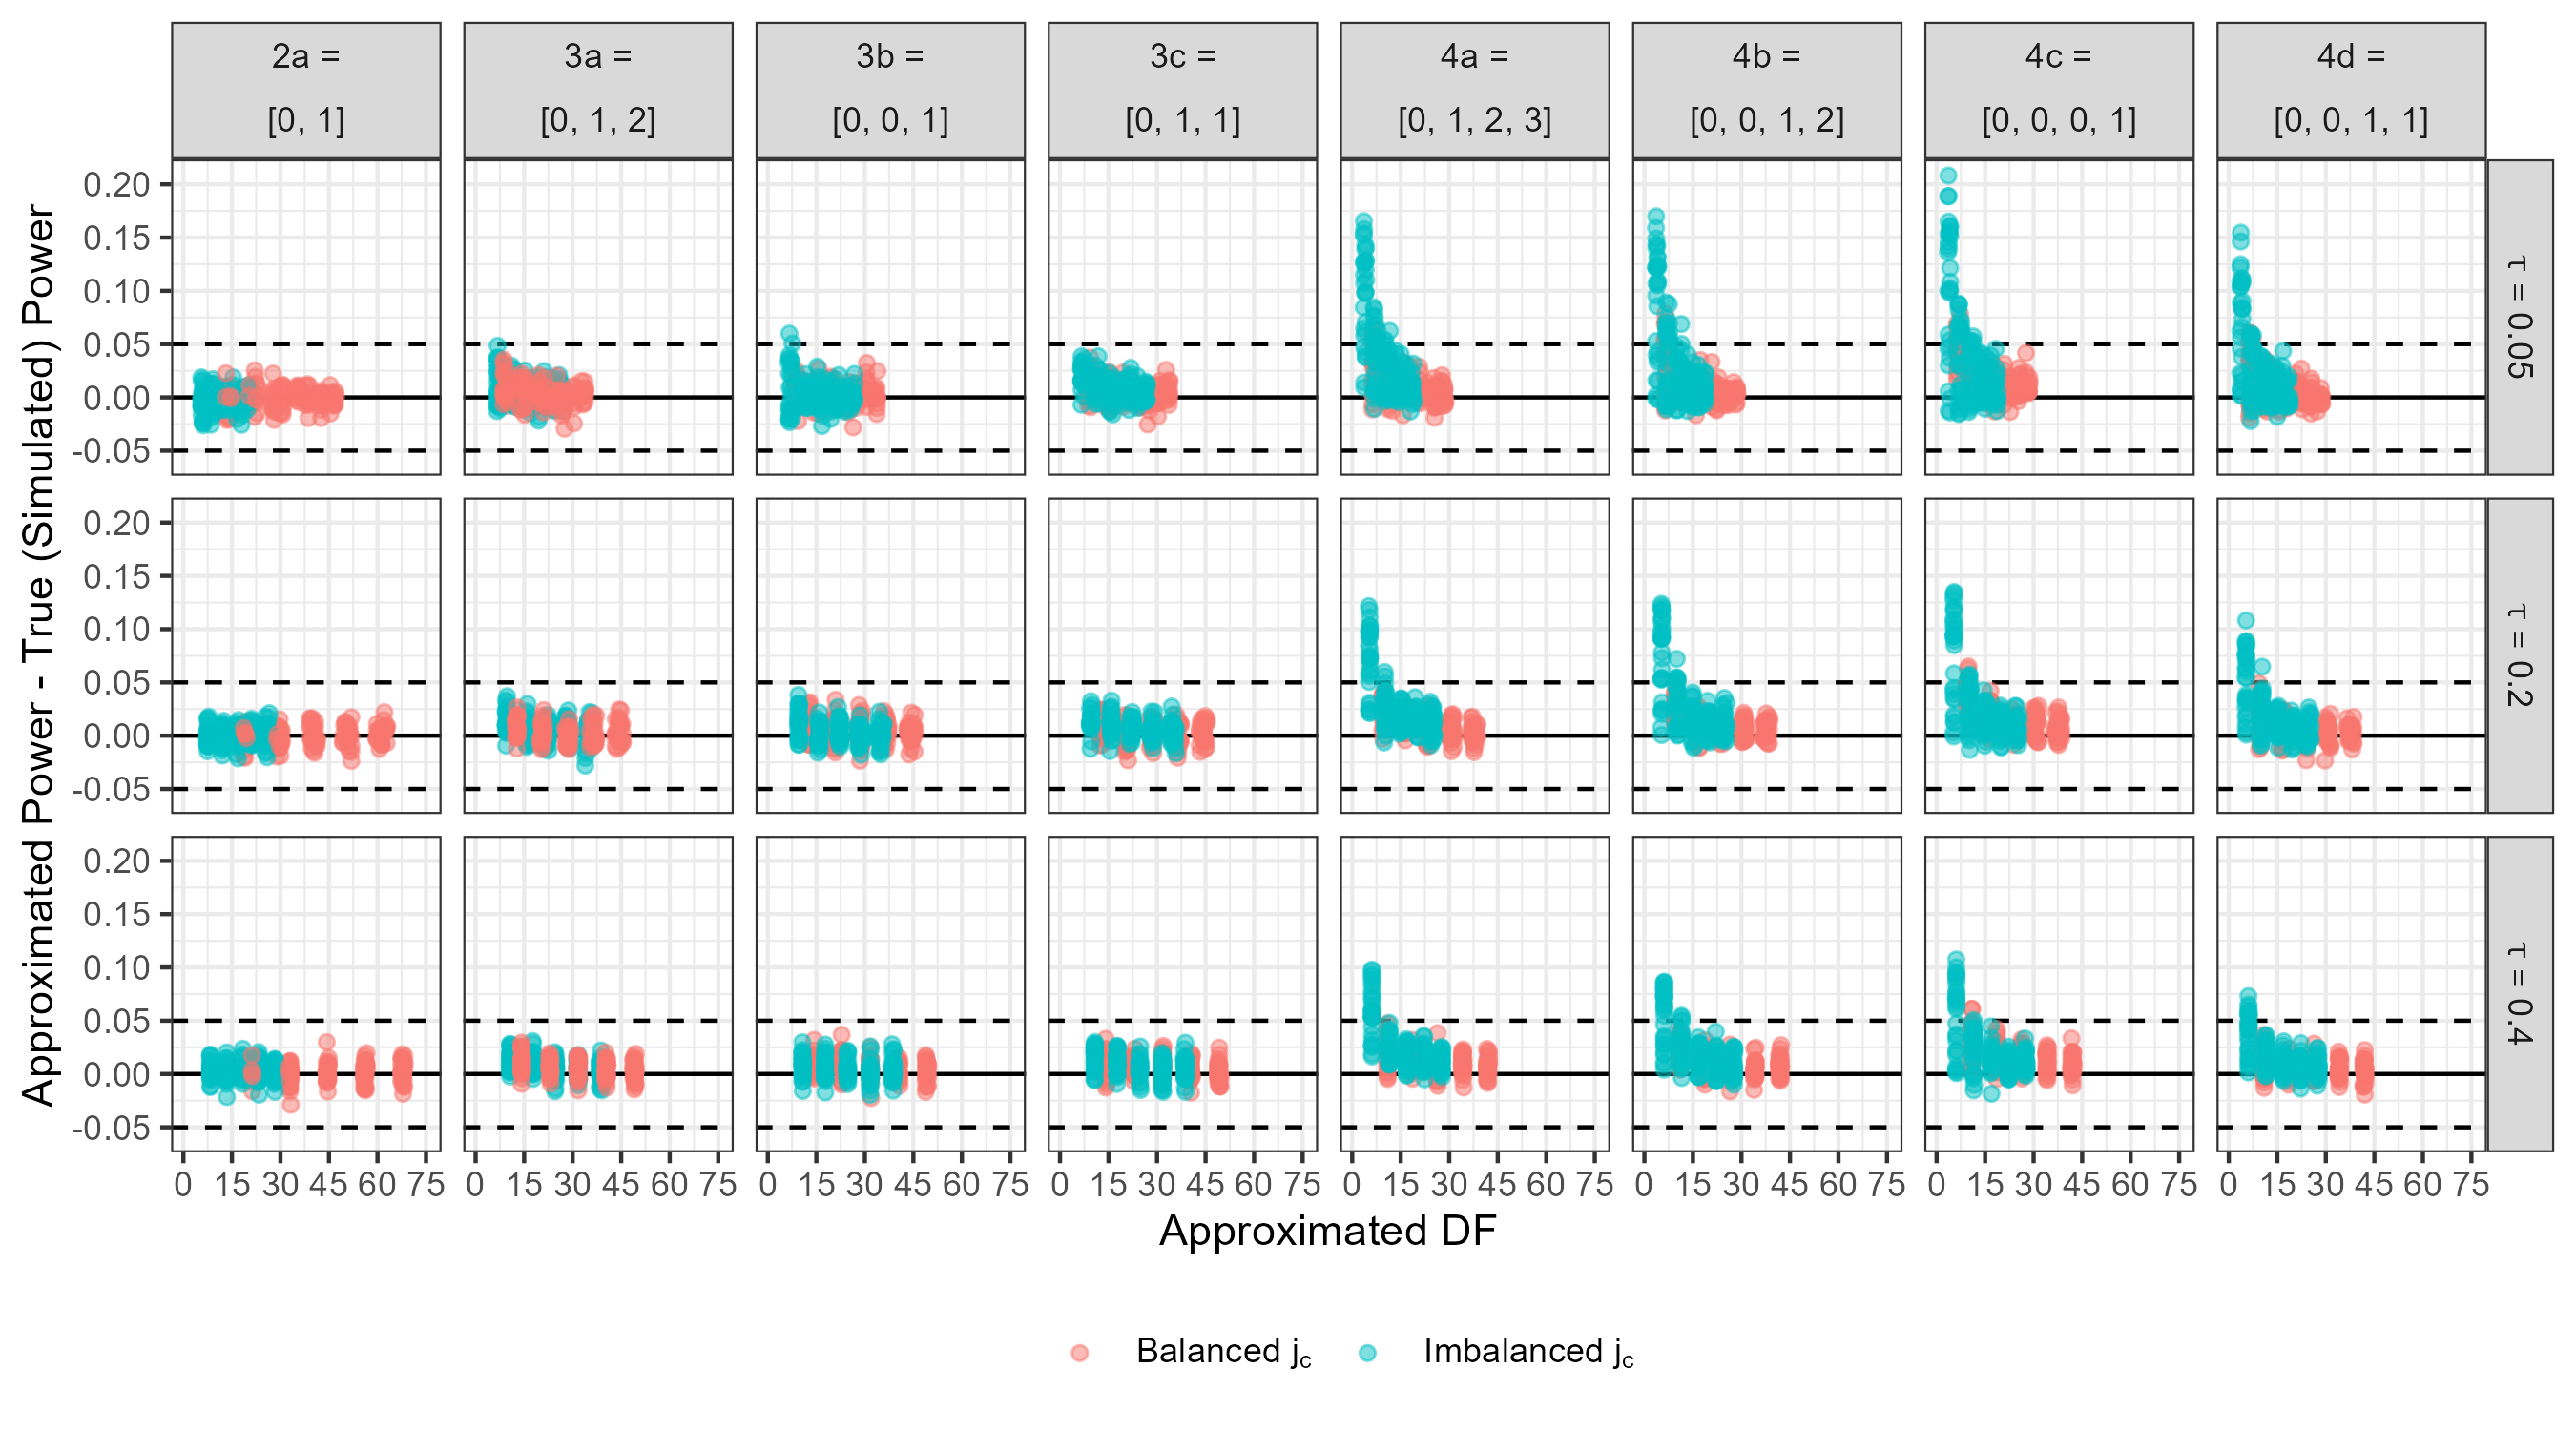
\includegraphics[width=\linewidth]{chapters/plots/df_mean.png}\caption{Power discrepancy between approximated power and true power vs. approximated degrees of freedom by pattern type ($f_c$), between-study heterogeneity ($\tau$), and the balance of number of studies per category (Balanced $j_c$ vs. Imbalanced $j_c$). The solid lines indicate no discrepancy between the approximated and simulated power. The dashed lines indicate that the approximated power over- or underestimated the true power by five percentage points. \label{fig: df_mean}}
    \vspace{-5pt}
\end{sidewaysfigure}  


\begin{sidewaysfigure}
    \centering
    \vspace{-5pt}
    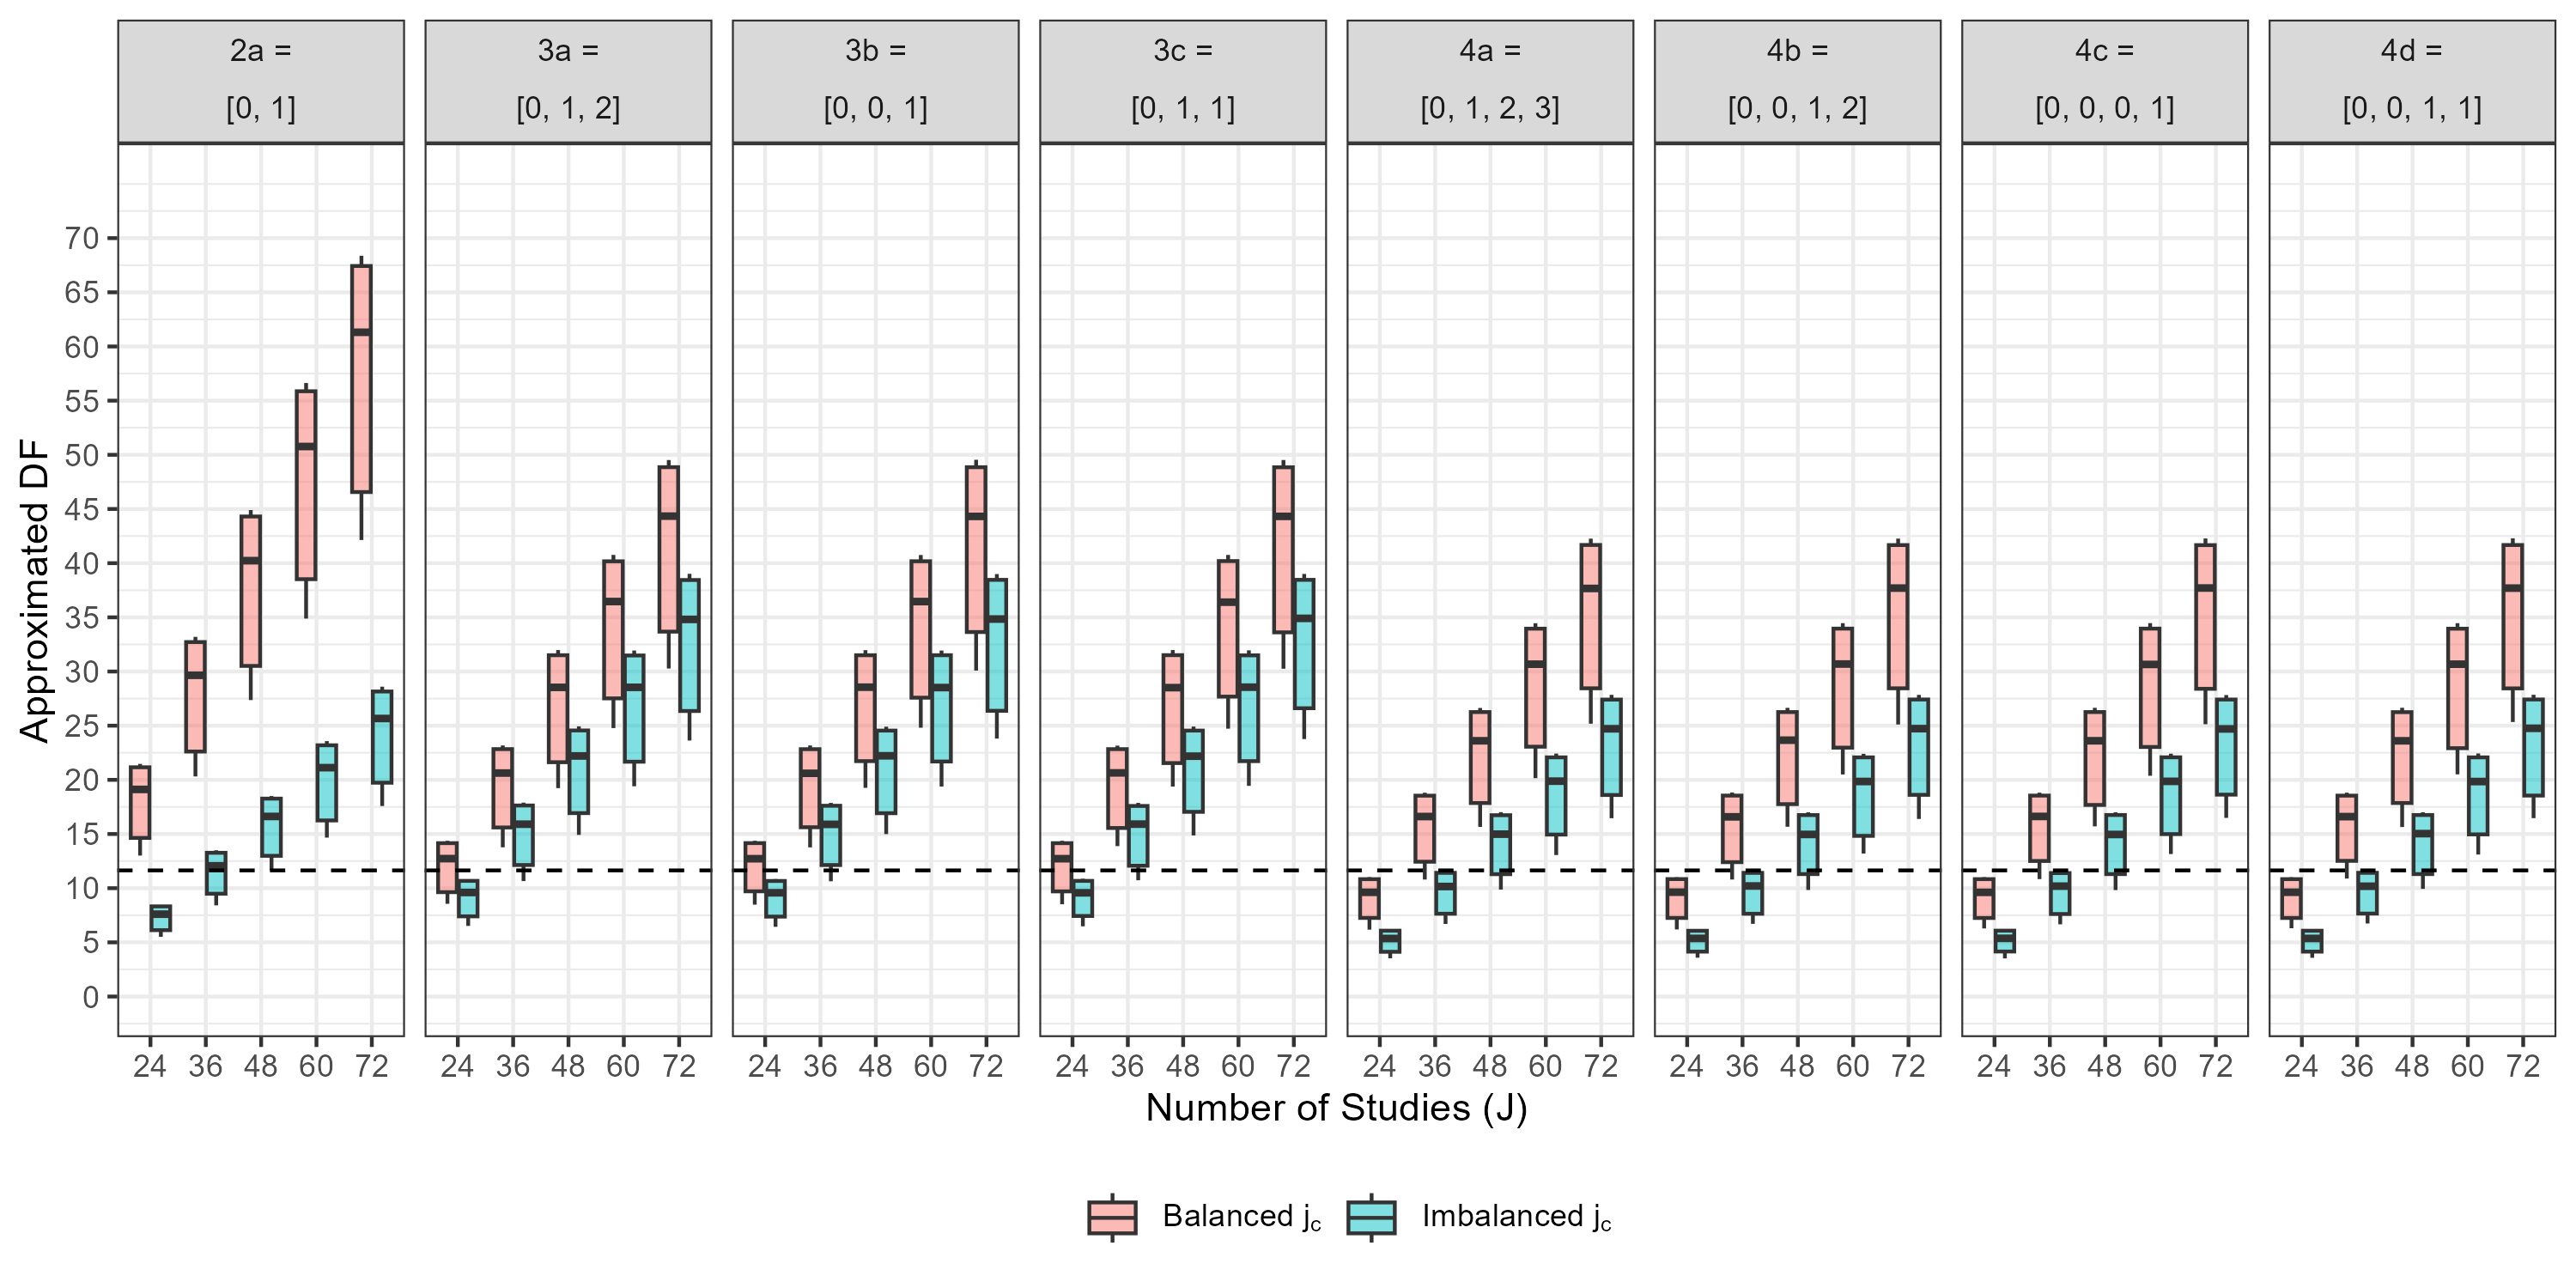
\includegraphics[width=\linewidth]{chapters/plots/dfvJ.png}
    \caption{Degrees of freedom of the approximation by the number of studies ($J$) by pattern type ($f_c$) by the balance of $j_c$. The dashed line represents the maximum $d_2$ value that resulted in a power discrepancy greater than five percentage points ($d_2 = 11.64$). \label{fig:dfvJ}}
    \vspace{-5pt}
\end{sidewaysfigure}

% \begin{sidewaysfigure}
%     \centering
%     \vspace{-5pt}
%     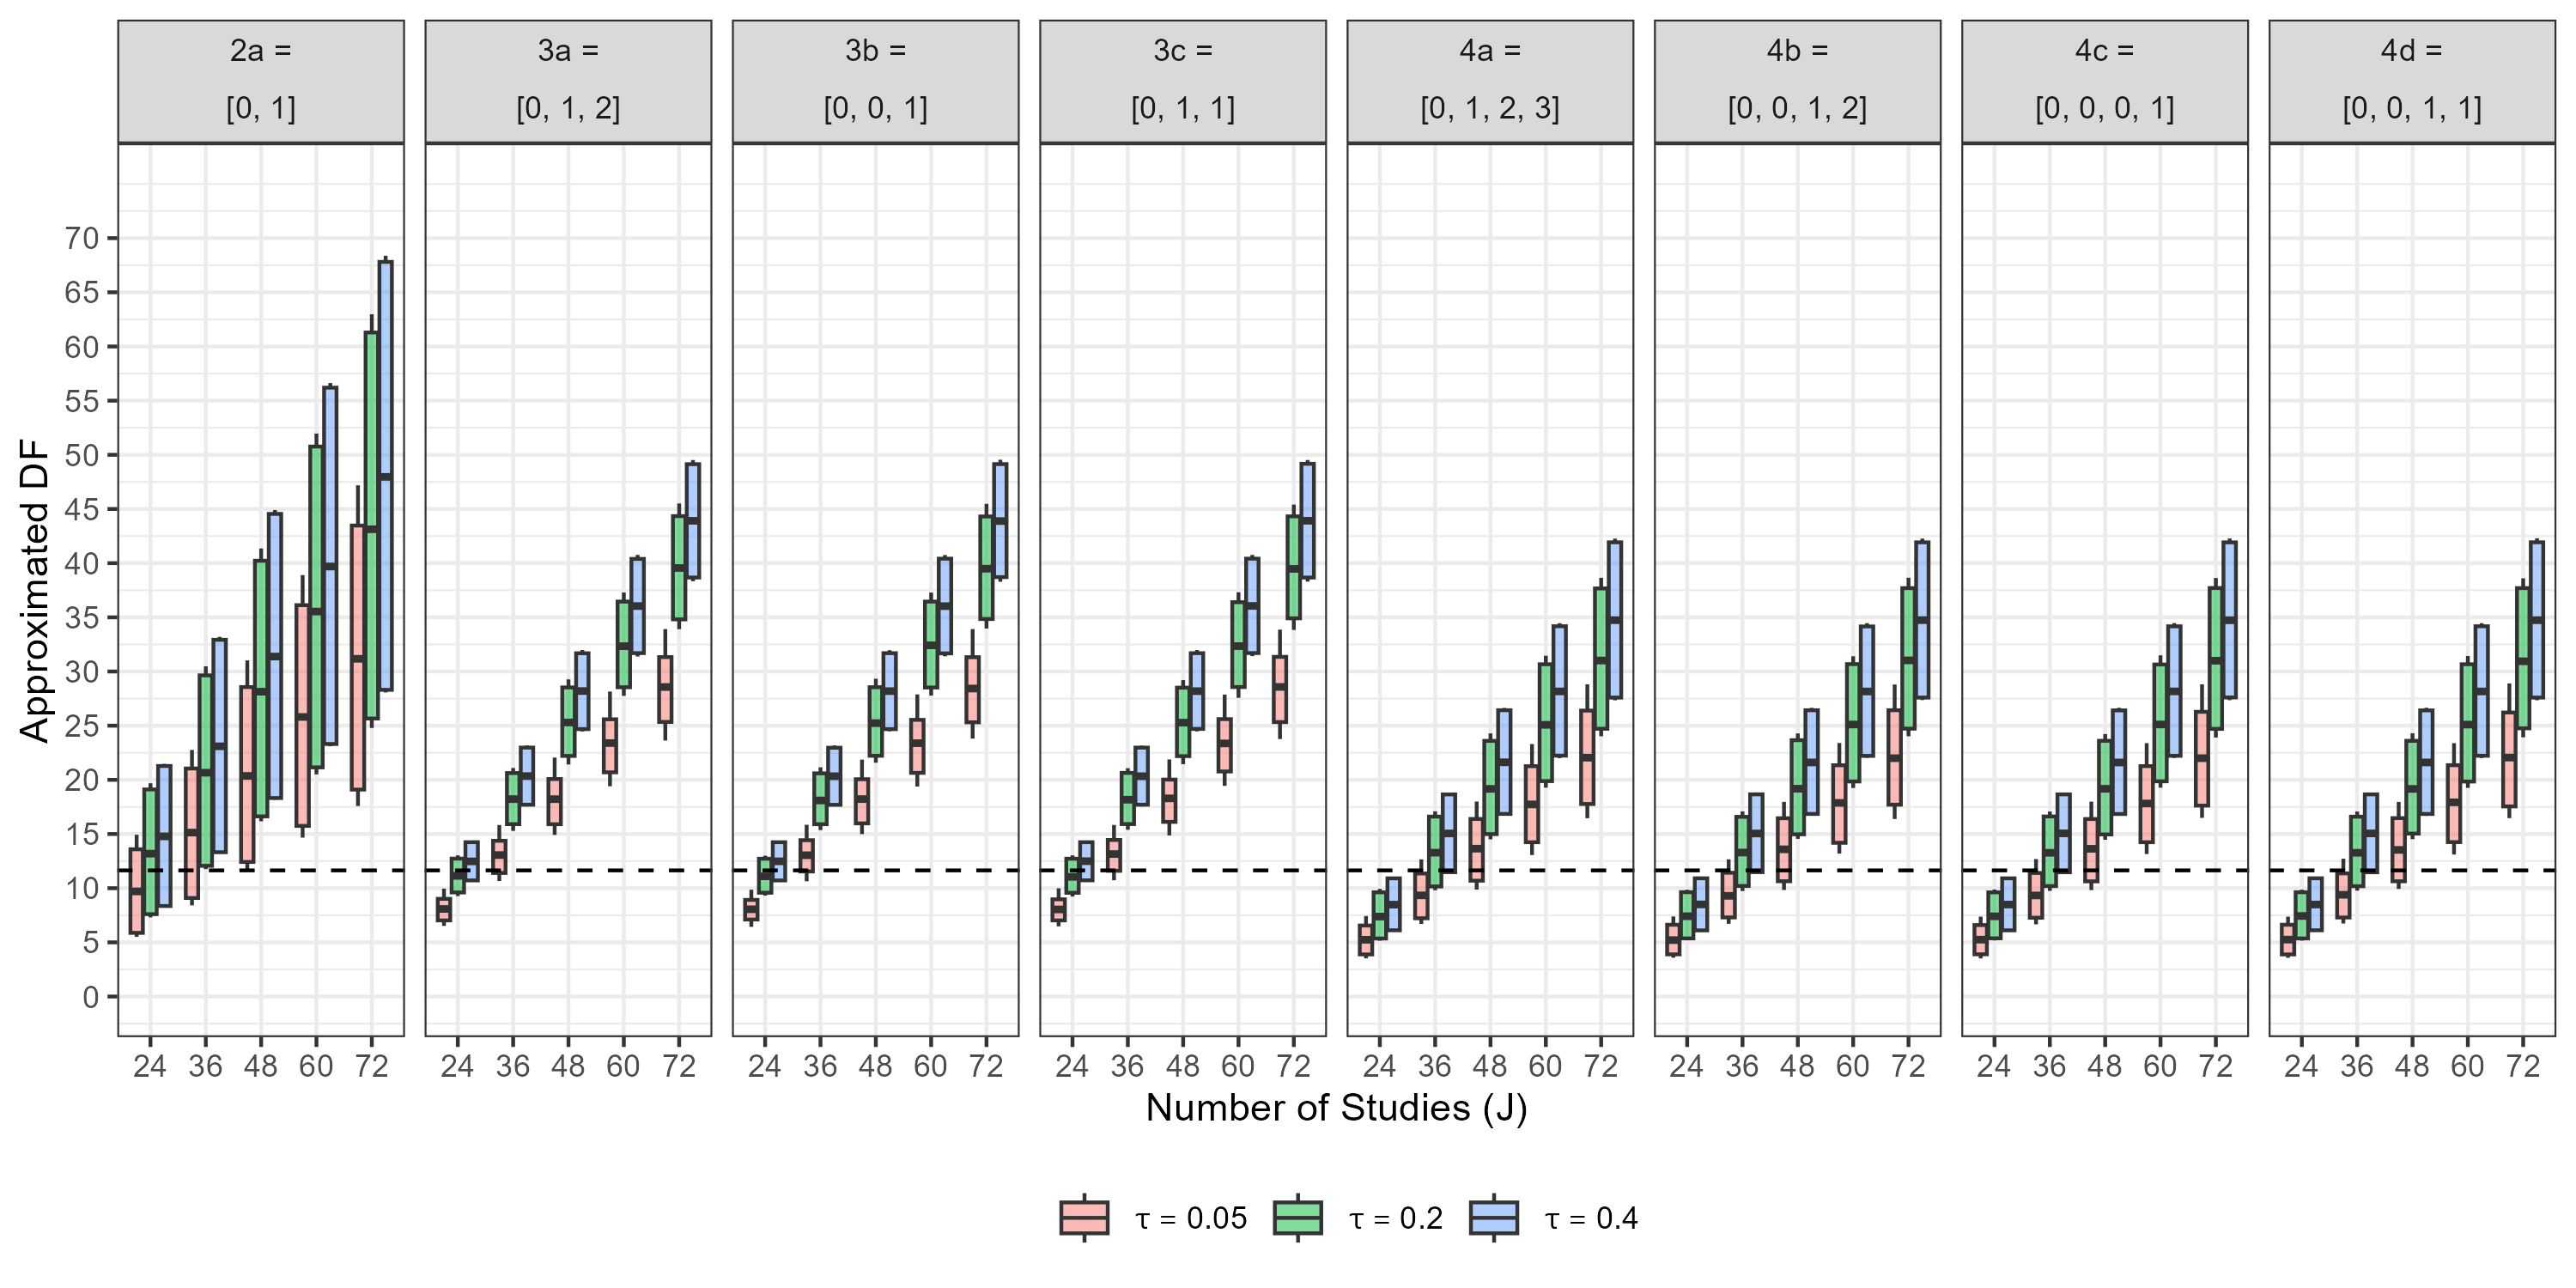
\includegraphics[width=\linewidth]{chapters/plots/dfvJ_tau.png}
%     \caption{Degrees of freedom of the approximation by the number of studies ($J$) by pattern type ($f_c$) by the between-study heterogeneity ($\tau$). The dashed line represents the maximum $d_2$ value that resulted in a power discrepancy greater than five percentage points ($d_2 = 11.64$). \label{fig:dfvJ_tau}}
%     \vspace{-5pt}
% \end{sidewaysfigure}

% \begin{sidewaysfigure}
%     \centering
%     \vspace{-5pt}
%     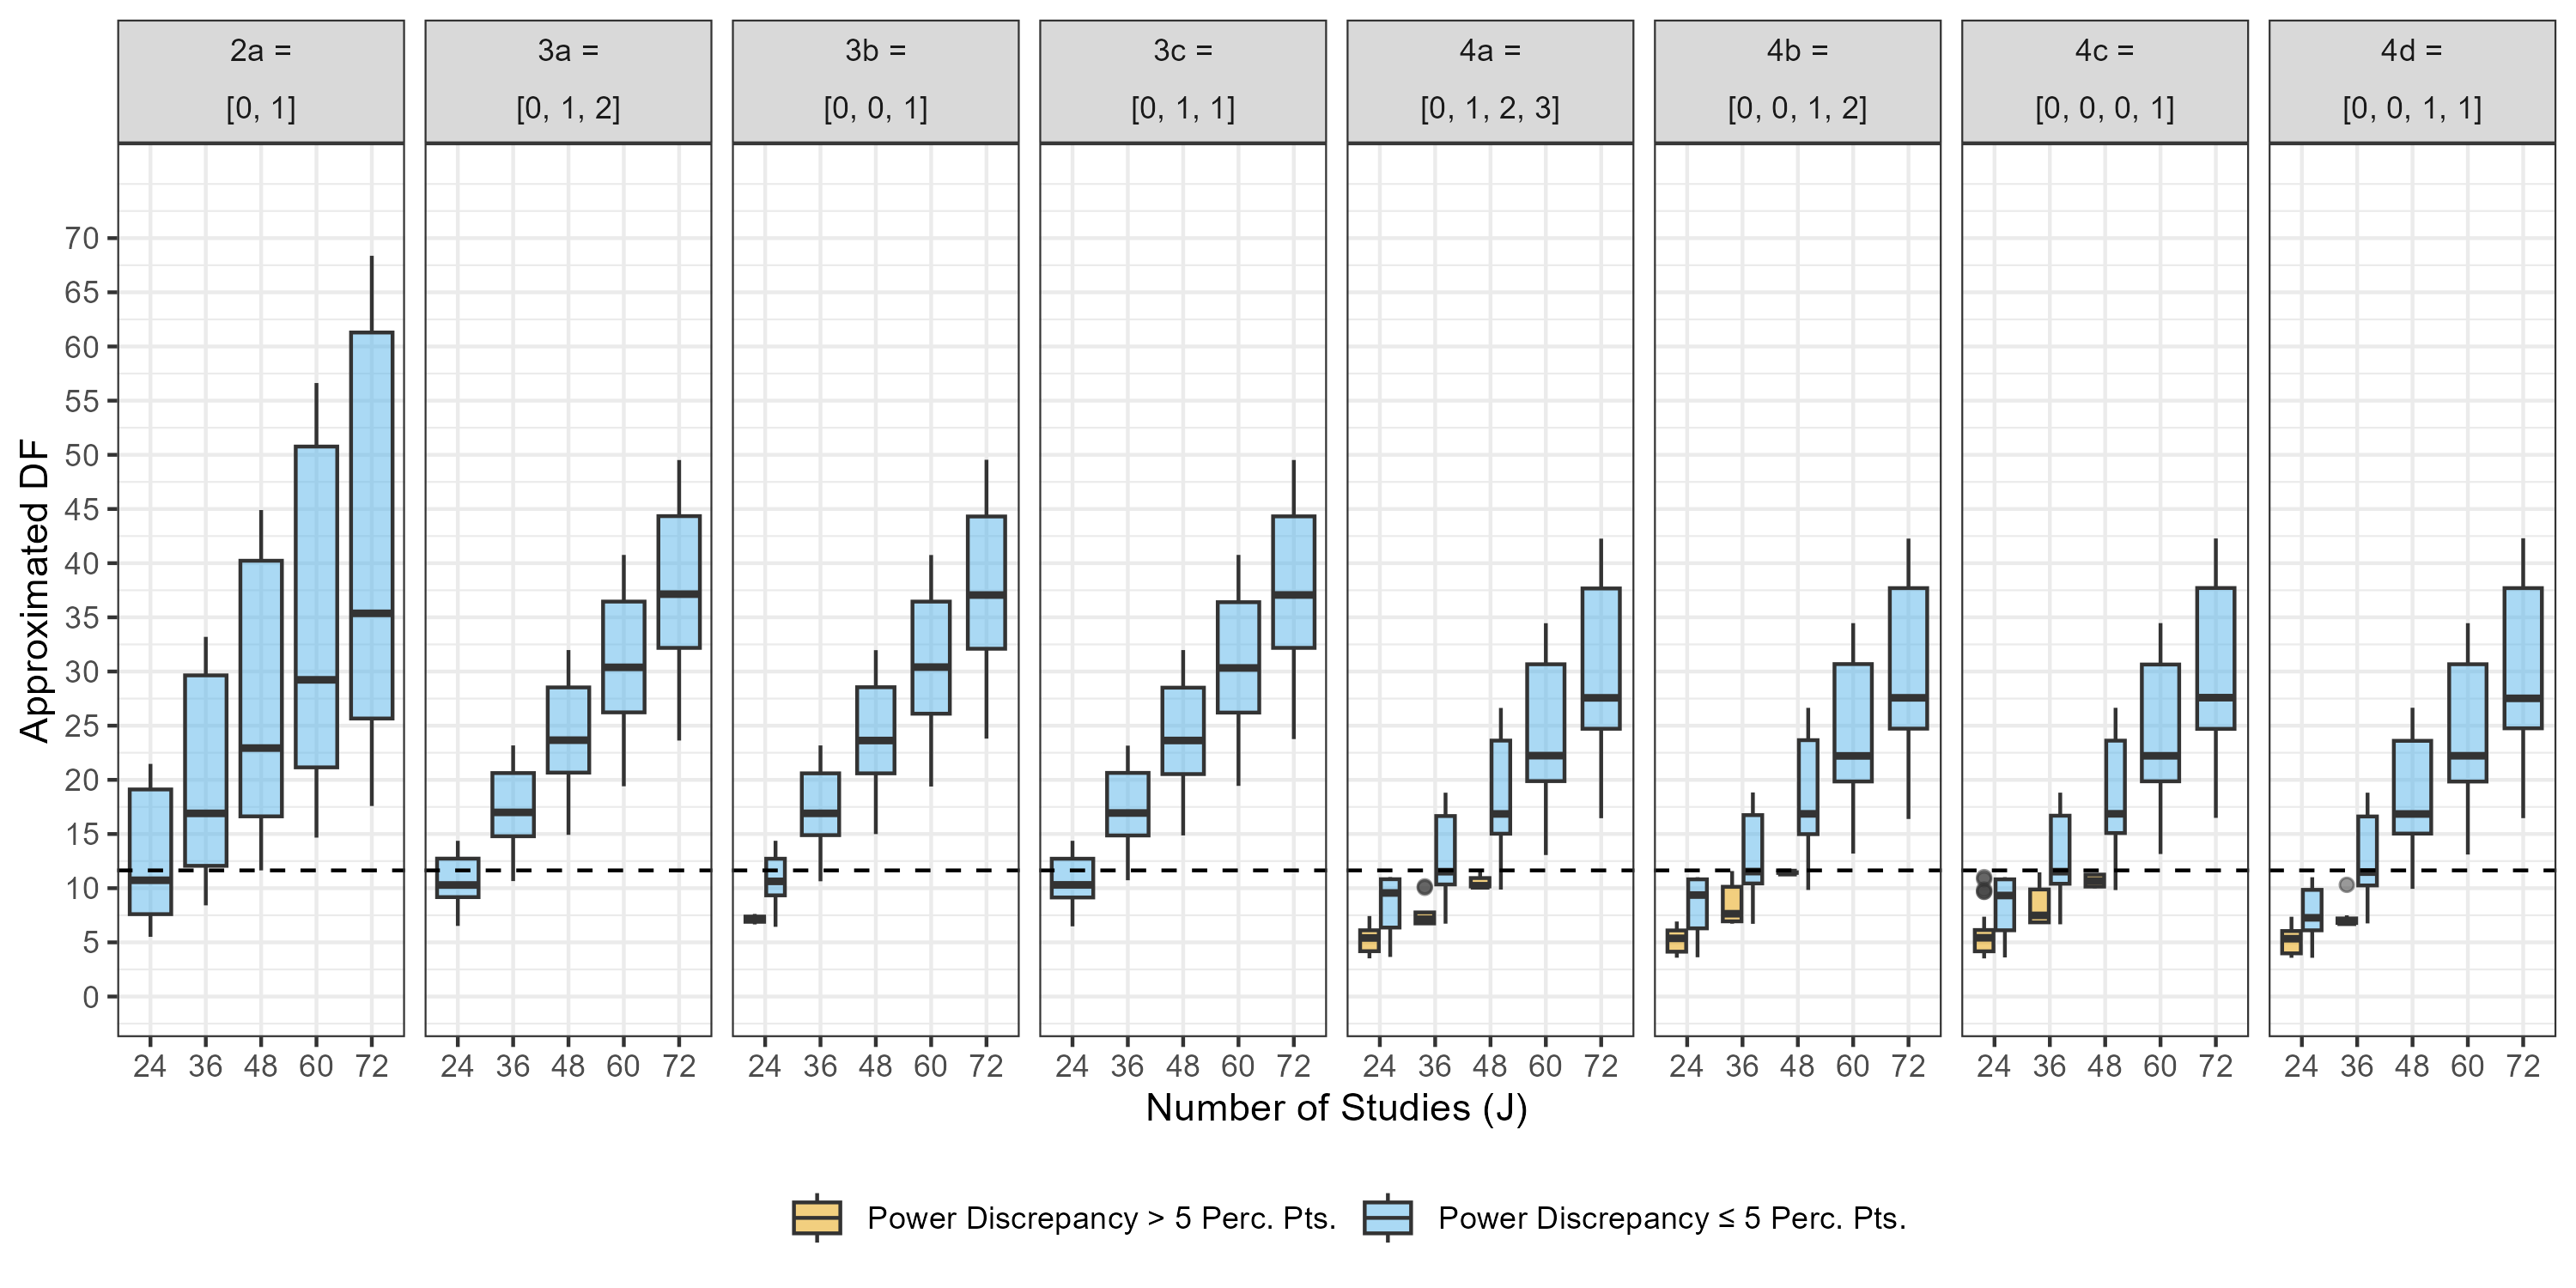
\includegraphics[width=\linewidth]{chapters/plots/dfvJ_pp.png}
%     \caption{Approximated degrees of freedom vs. the number of studies ($J$) by pattern type ($f_c$). The color indicates if the approximated power overestimated the true power by 5 percentage points or not.  The dashed line indicates the maximum $d_2$ value that resulted in a power discrepancy greater than five percentage points ($d_2 = 11.64$). Note: No power estimates from the approximation underestimated power by more than five percentage points. \label{fig:dfvJ_pp}}
%     \vspace{-5pt}
% \end{sidewaysfigure}


Finally, even though the analysis of deviance in Section \ref{sec: analysis of deviance - empirical} found that $\omega$ and $\rho$ explained little variation in the power discrepancies, I chose to create Figure \ref{fig: fc_rho_omega_empirical}. This figure has the approximated power on the x-axis, the pattern of the $\mu_c$ and $\rho$ as facets, and $\omega$ mapped to the color. The figure shows that neither the sampling correlation, $\rho$, nor the within-study variance, $\omega$, has an impact on the accuracy of the approximation.

\begin{sidewaysfigure}
    \centering
    \vspace{-5pt}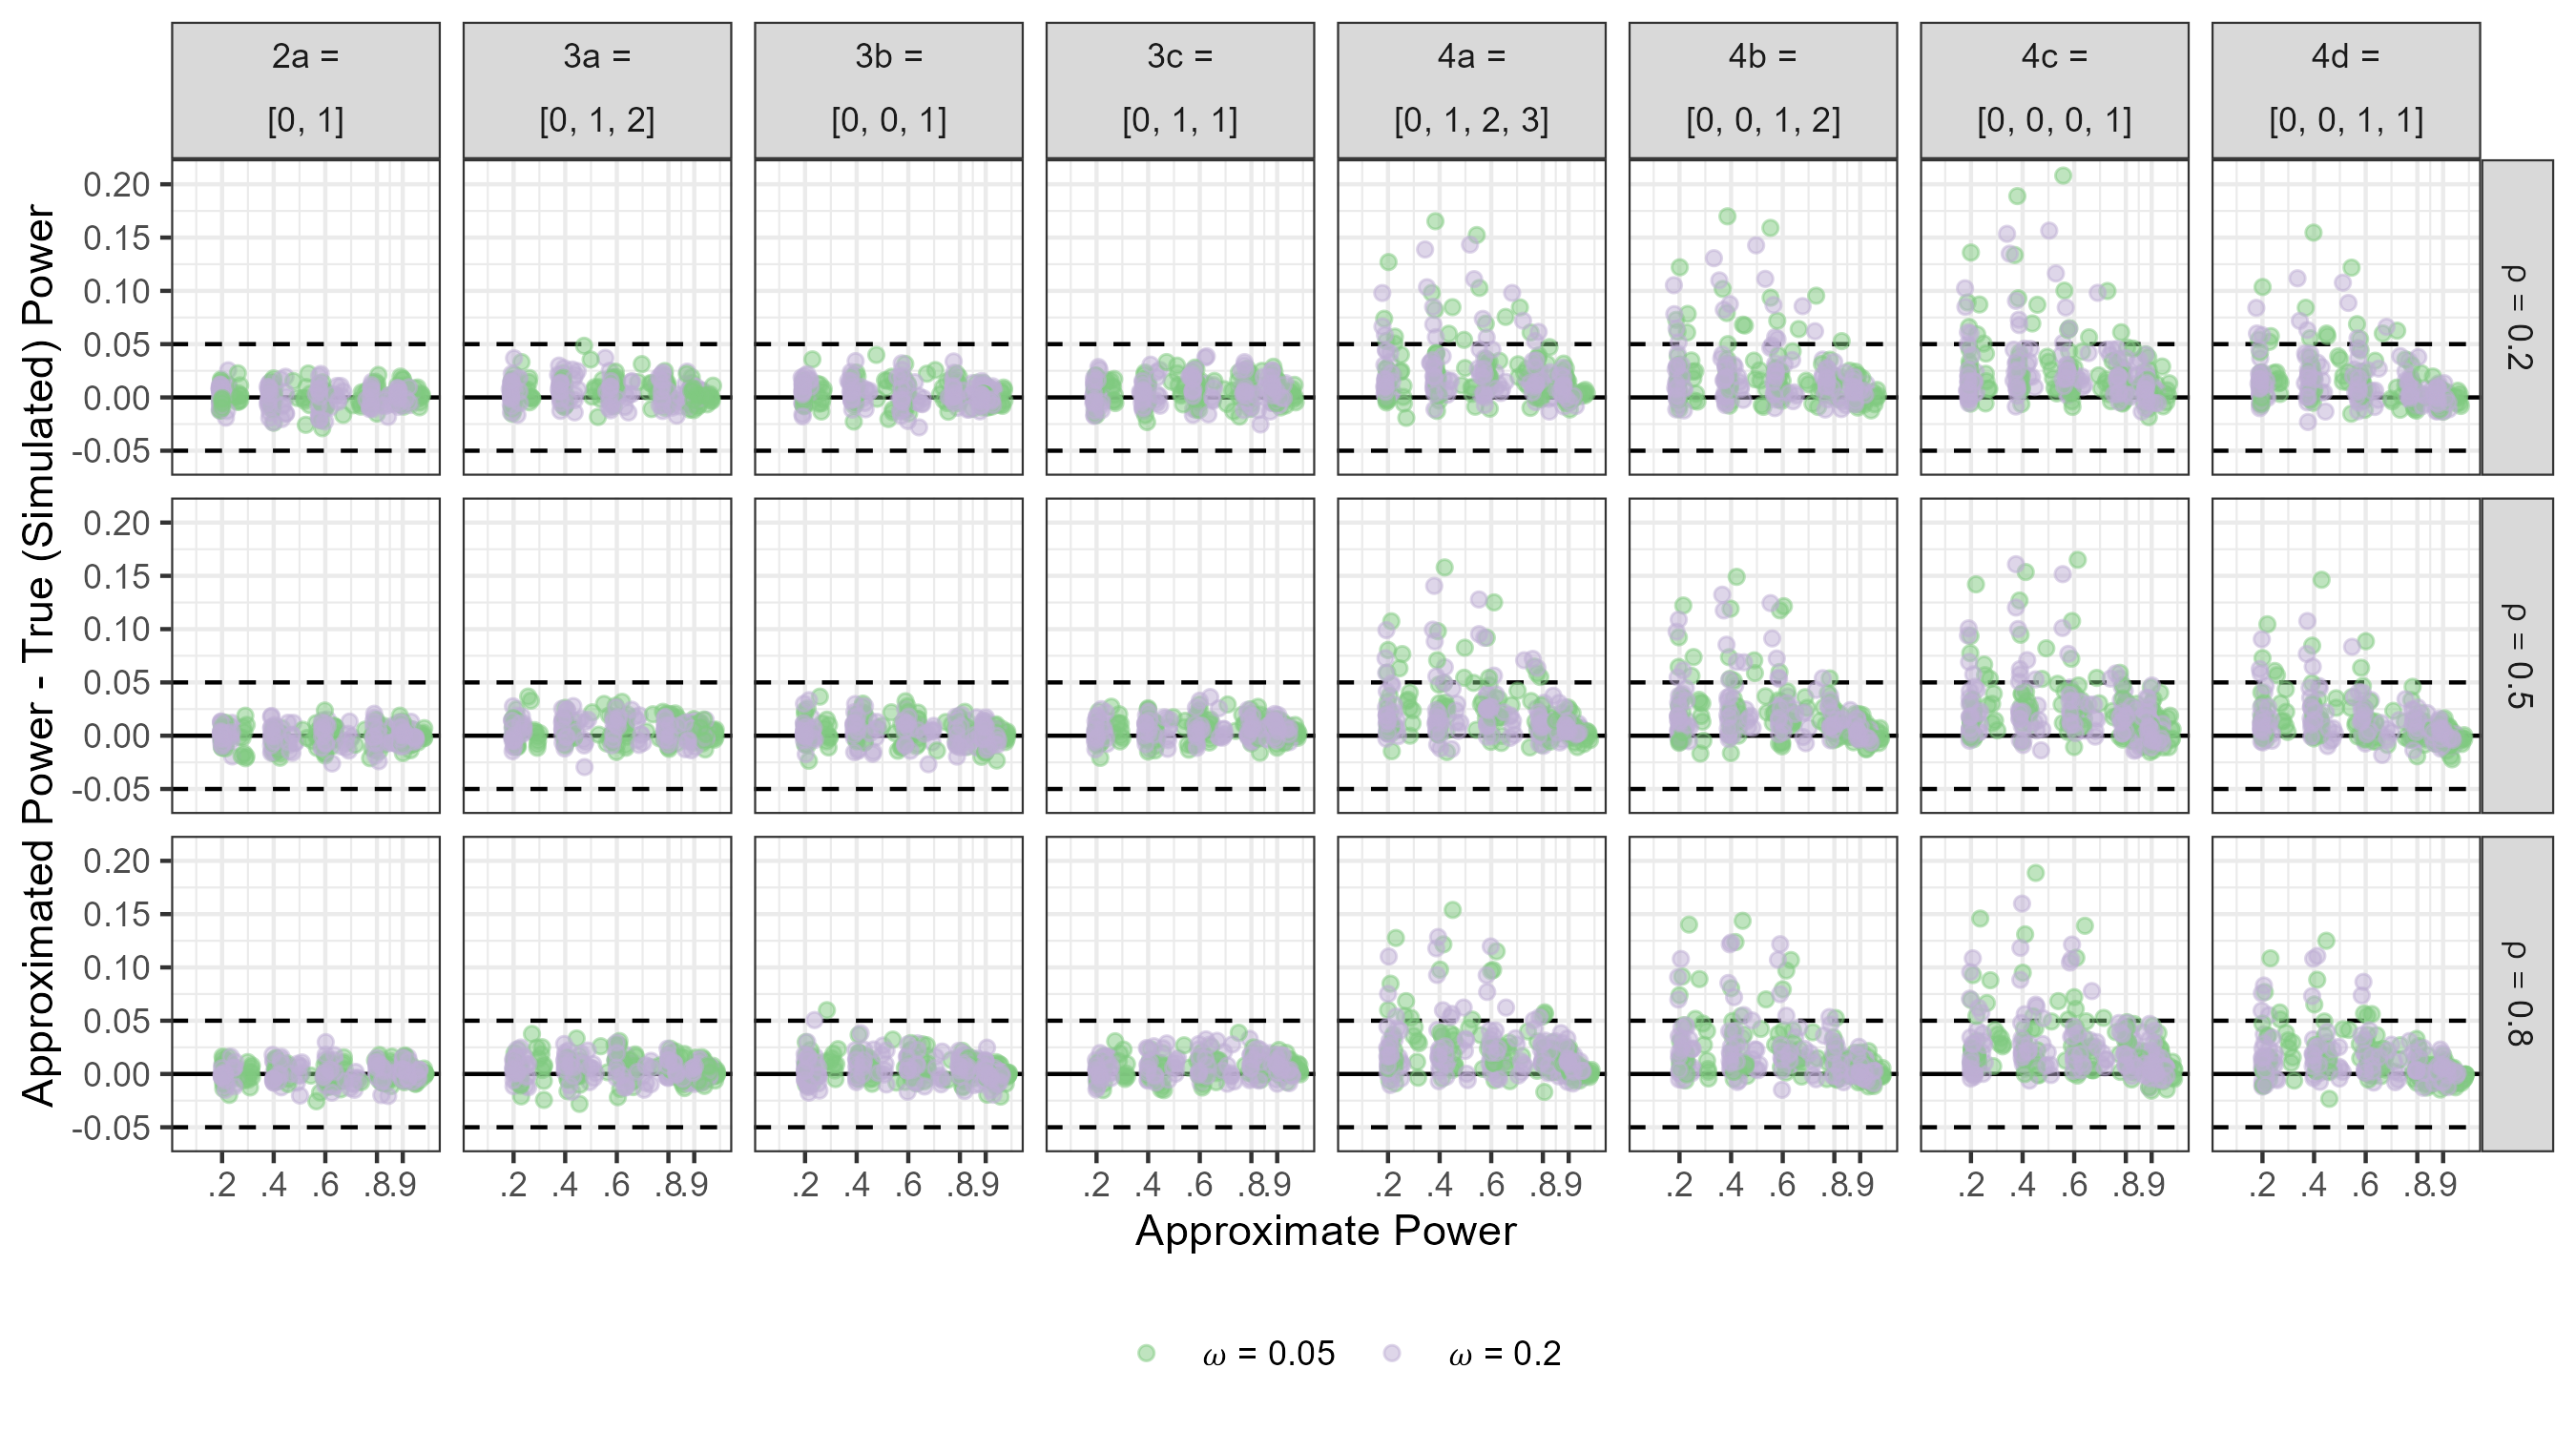
\includegraphics[width=\linewidth]{chapters/plots/fc_rho_omega_empirical.png}\caption{Power discrepancy between approximation power and true power vs. approximated power by pattern type ($f_c$), sample correlation ($\rho$), and within-study variation ($\omega$). The solid lines indicate no discrepancy between the approximated and simulated power. The dashed lines indicate that the approximated power over- or underestimated the true power by five percentage points.}
    \label{fig: fc_rho_omega_empirical}
    \vspace{-5pt}
\end{sidewaysfigure}

%%%%%%%%%%%%%%%%%%%%%%%%%%%%%%%%%%%%%%%%

\subsection{Approximation Performance Across Sampling/Imputation Methods}

I also examined differences in the power discrepancies across sampling/imputation methods for the primary study characteristics when making assumptions about the number of effect sizes ($k_j$) and the sampling variances ($\sigma_j^2$) in the approximation. I found that the performance of the approximation when using the stylized sampling method was similar to that of the empirical sampling method across all conditions. 
This is probably due to how well the stylized distributions fit the empirical distributions, as seen in Figures \ref{fig:densitysigma_sq} and \ref{fig:pmfkj}. In most conditions, the balanced assumption method underestimated the true power. However, when $J=24$ and $C=4$, the power estimates from the balanced assumption method overestimated the true power to about the same degree as the empirical and stylized sampling methods.

Figures \ref{fig: fc_bal_allsamp_rejrate}, \ref{fig: fc_bal_allsamp_rejrate_J24}, \ref{fig: allsamp_bal_J72}, \ref{fig: allsamp_tau}, \ref{fig: fc_omega_all_samp_rejrate}, and \ref{fig: fc_rho_all_samp_rejrate} present the results of the power discrepancies under the three different assumptions of the primary study characteristics. To compare across the sampling/imputation methods, instead of graphing the approximated power on the x-axis as in the last section, the rejection rate (true power) is mapped to the x-axis. The reason I changed the x-axis is because for the balanced assumption method the power estimates that result from the approximation will return the power neighborhood value since the $\mu_c$ were generated the same way, so using the simulated power as the x-axis ensures that it is the same point of comparison for all three methods. 

%how closely does the approximate power with balanced condition correspond to real power, when the real simulated power level is based on heterogeneous study characteristics? 

In Figure \ref{fig: fc_bal_allsamp_rejrate}, patterns of the $\mu_c$ and the sampling/imputation methods are mapped onto facets, and the balance of the $j_c$ is mapped onto color. Regarding the difference in the performance of the approximation using different sampling methods for the $k_j$ and $\sigma_j^2$, the figure shows that there are minimal differences between the empirical and stylized sampling methods. Both sampling methods resulted in samples where the approximation overestimated the true power beyond five percentage points when $C = 4$ and there was imbalanced $j_c$ across the categories. Across all conditions, the empirical sampling method performed better, as expected. For example, as can be seen in Figure \ref{fig: fc_bal_allsamp_rejrate_J24}, when the power neighborhood is $P = 0.9$ and the number of studies was $J= 24$, only the stylized sampling method resulted in samples that overestimated the true power. For the empirical sampling method, across conditions, the approximation at most underestimated the true power by $2.94$ percentage points and overestimated the power by $20.82$ percentage points. For the stylized sampling method, the approximation at most underestimated the true power by $3.16$ percentage points and overestimated the power by $25.72$ percentage points. In cases where the empirical sampling method was accurate (within $\pm 5$ percentage points), the stylized method did overestimate the true power by more than five percentage points in some conditions. This happened when $C = 3$ and $J \leq 36$ by as much as 8.85 percentage points. 

Because I generated the $\mu_c$ using the mean $\sigma_j^2$ and mean $k_j$ of the empirical distributions from the \textcite{WilliamsRyan2022HiMI} dataset, the approximation with balanced characteristics returns the exact value of the power neighborhood factor I used to generate the $\mu_c$ for that condition. Figure \ref{fig: fc_bal_allsamp_rejrate} shows how much the true power is off from the power neighborhood factor used in that condition. For example, across all conditions with a power neighborhood value of $P = 0.6$, the true power was at most $25.3$ percentage points above and $24.2$ percentage points below a power of $60\%$ (which were the biggest discrepancies for the balanced assumption method as well). Assuming balanced study characteristics results in power estimates that overestimate around the same magnitude as the stylized (max overestimation is $25$ percentage points) when $C=4$ and $J=24$ (see Figure \ref{fig: fc_bal_allsamp_rejrate_J24}). However, unlike the other methods, the balanced method underestimates power across the rest of the conditions. For example, Figure \ref{fig: allsamp_bal_J72} displays discrepancies in power versus true power faceted by $f_c$ and the sampling/imputation methods with balance of $j_c$ as the color when $J=72$. As seen in this graph, while the stylized and the empirical sampling methods result in accurate approximations across all the values of $f_c$, the balanced method results in power estimates much smaller than the true power.  Neither the balance of the $j_c$ nor the $f_c$ explains the underestimation, because the power discrepancy for the balanced assumption method does not vary by these factors. 

The magnitude of the discrepancy for the balance assumption method when it underestimates the true power appears to be impacted by the value of the power neighborhood, with the largest discrepancies occurring around $P = .4$ and $P = .6$. Furthermore, the between-study heterogeneity also seems to impact the degree of the underestimation of the true power for the balanced assumption method. Figure \ref{fig: allsamp_tau} displays the discrepancies in approximated power compared to true power with $f_c$ and the sampling/imputation methods mapped onto facets and between-study heterogeneity ($\tau$) mapped onto color. The figure shows that the value of $\tau$ impacts the discrepancy for the balanced assumption method, where the true power estimate is consistently greater than the power estimate of the approximation when $\tau = 0.05$ across all $f_c$.


\begin{sidewaysfigure}
    \centering
    \vspace{-5pt}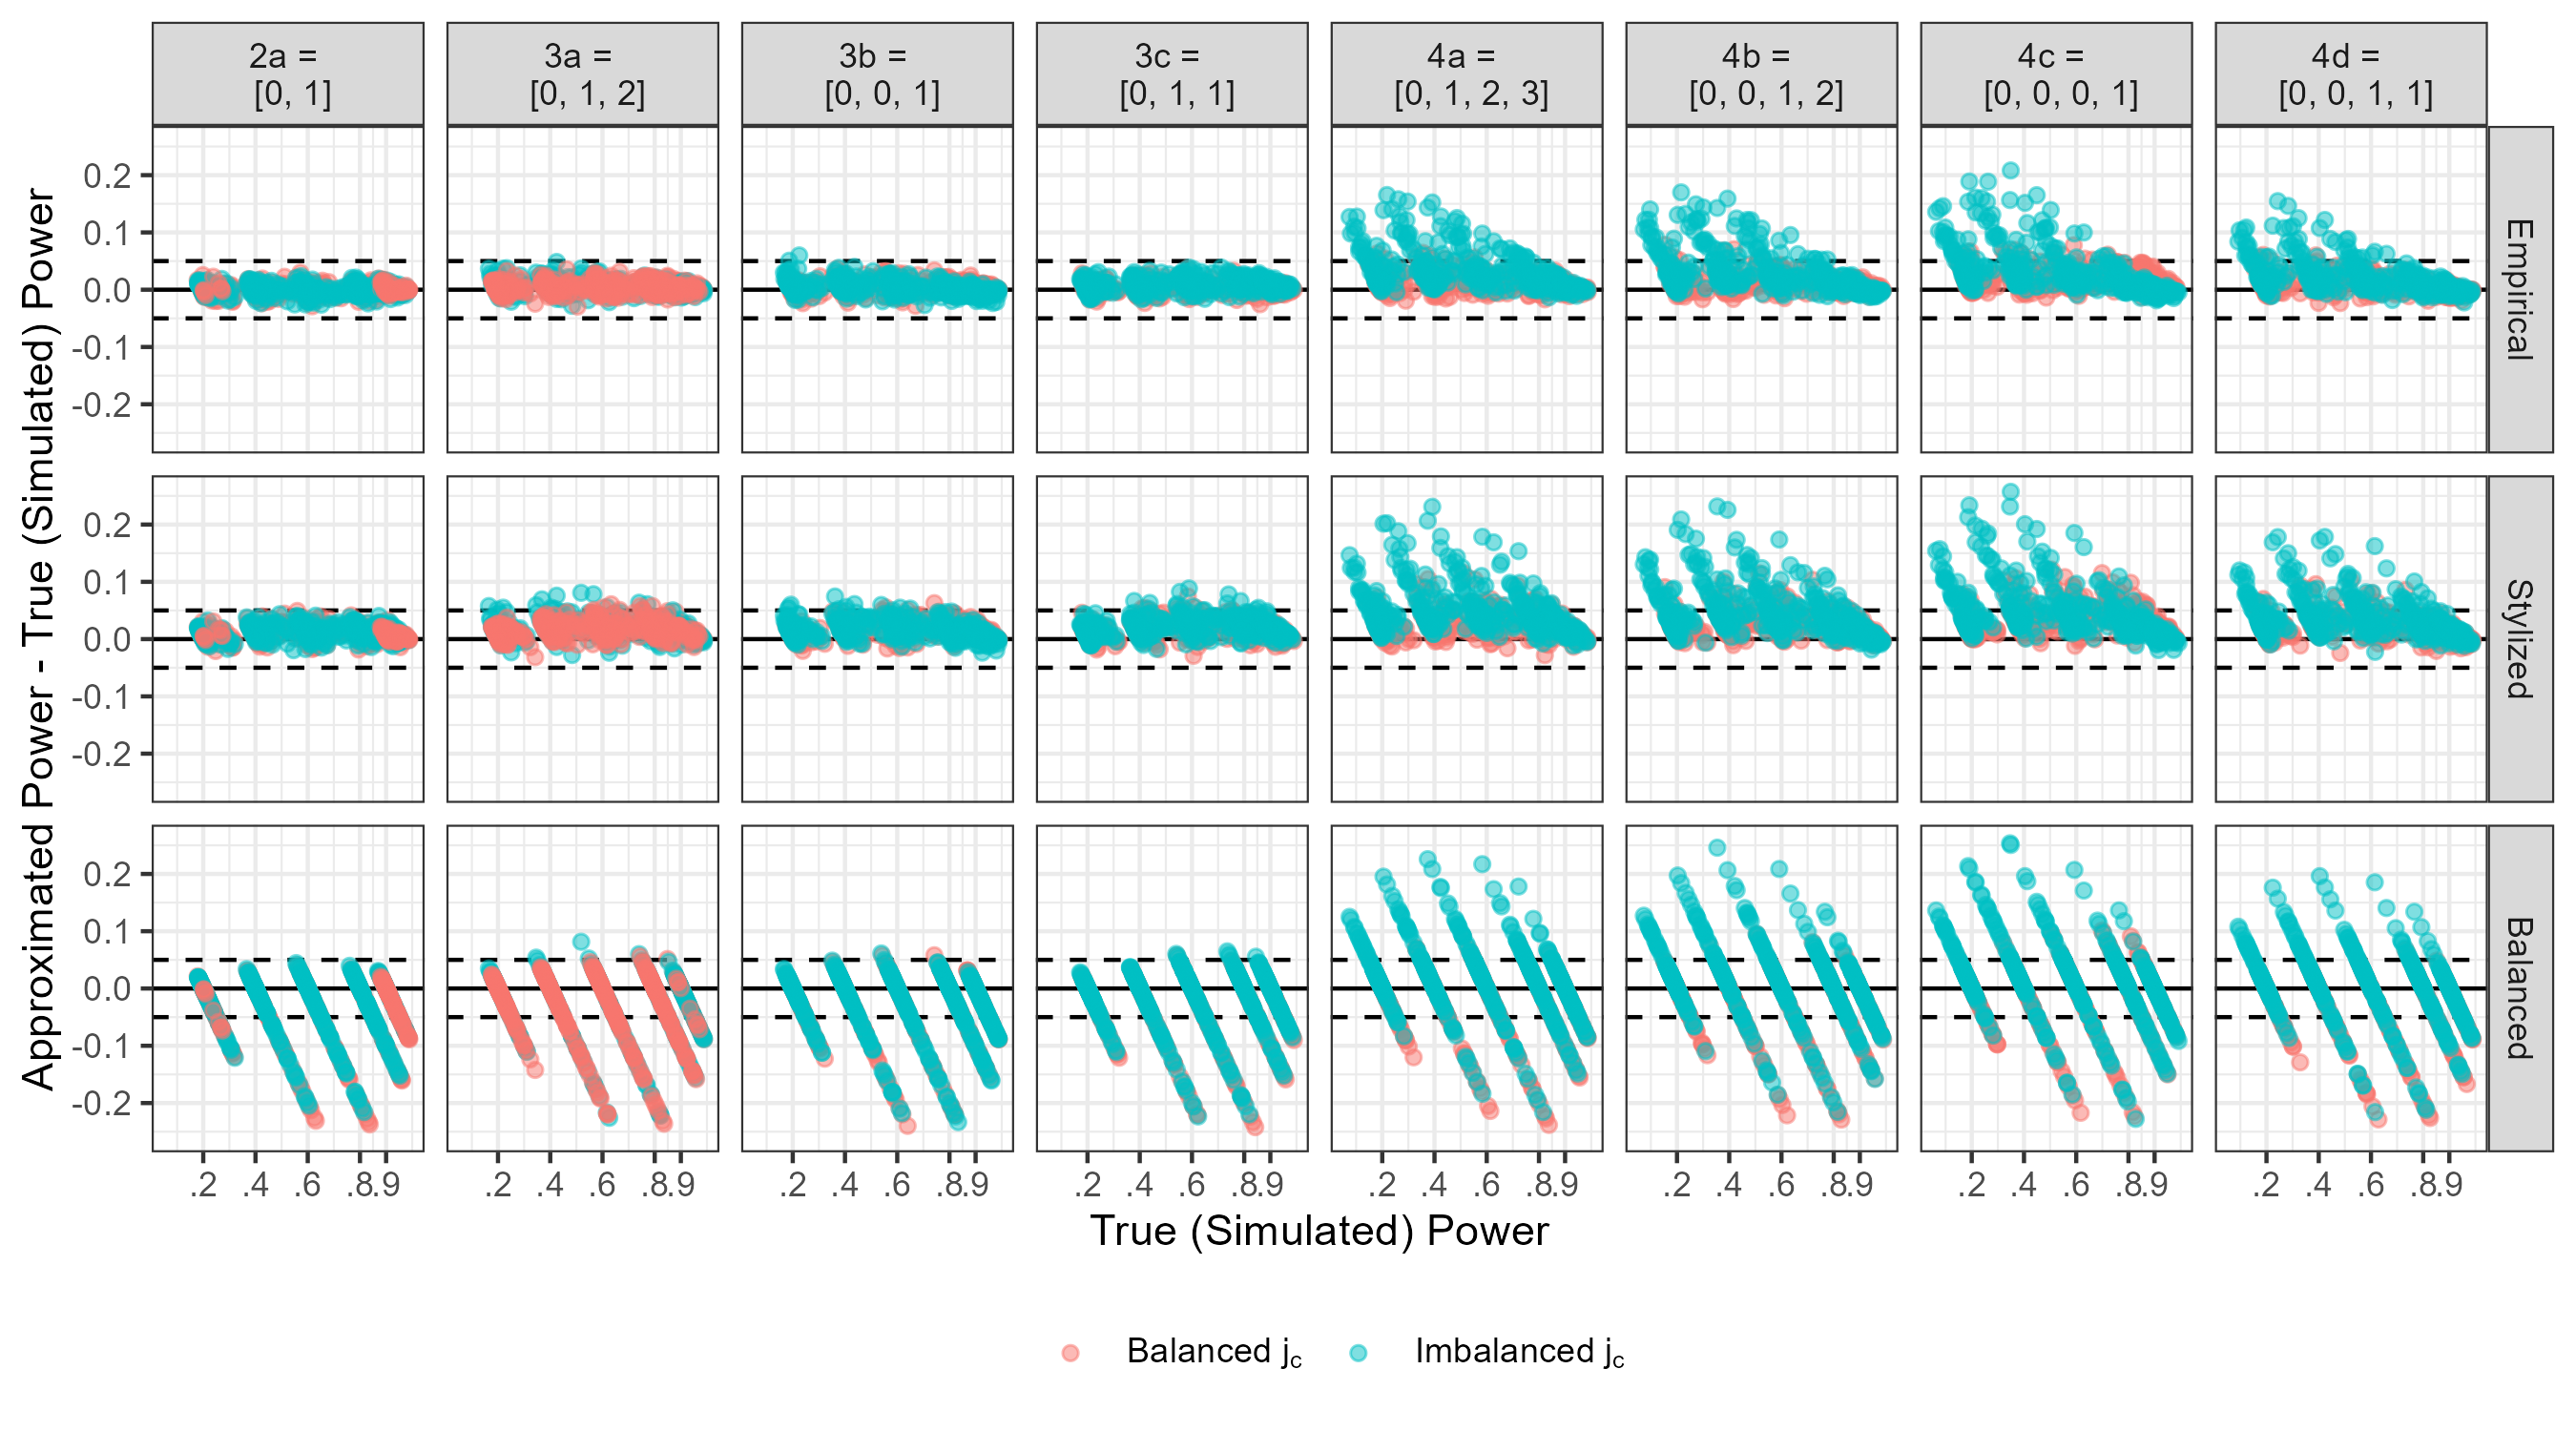
\includegraphics[width=\linewidth]{chapters/plots/fc_bal_allsamp_rejrate.png}\caption{Power discrepancy between approximation power and true power vs. true power by pattern type ($f_c$), sampling/imputation methods for the primary study characteristics, and the balance of the number of studies per category (Balanced $j_c$ vs. Imbalanced $j_c$).The solid lines indicate no discrepancy between the approximated and simulated power. The dashed lines indicate that the approximated power over- or underestimated the true power by five percentage points.\label{fig: fc_bal_allsamp_rejrate}}
    \vspace{-5pt}
\end{sidewaysfigure}

\begin{sidewaysfigure}
    \centering
    \vspace{-5pt}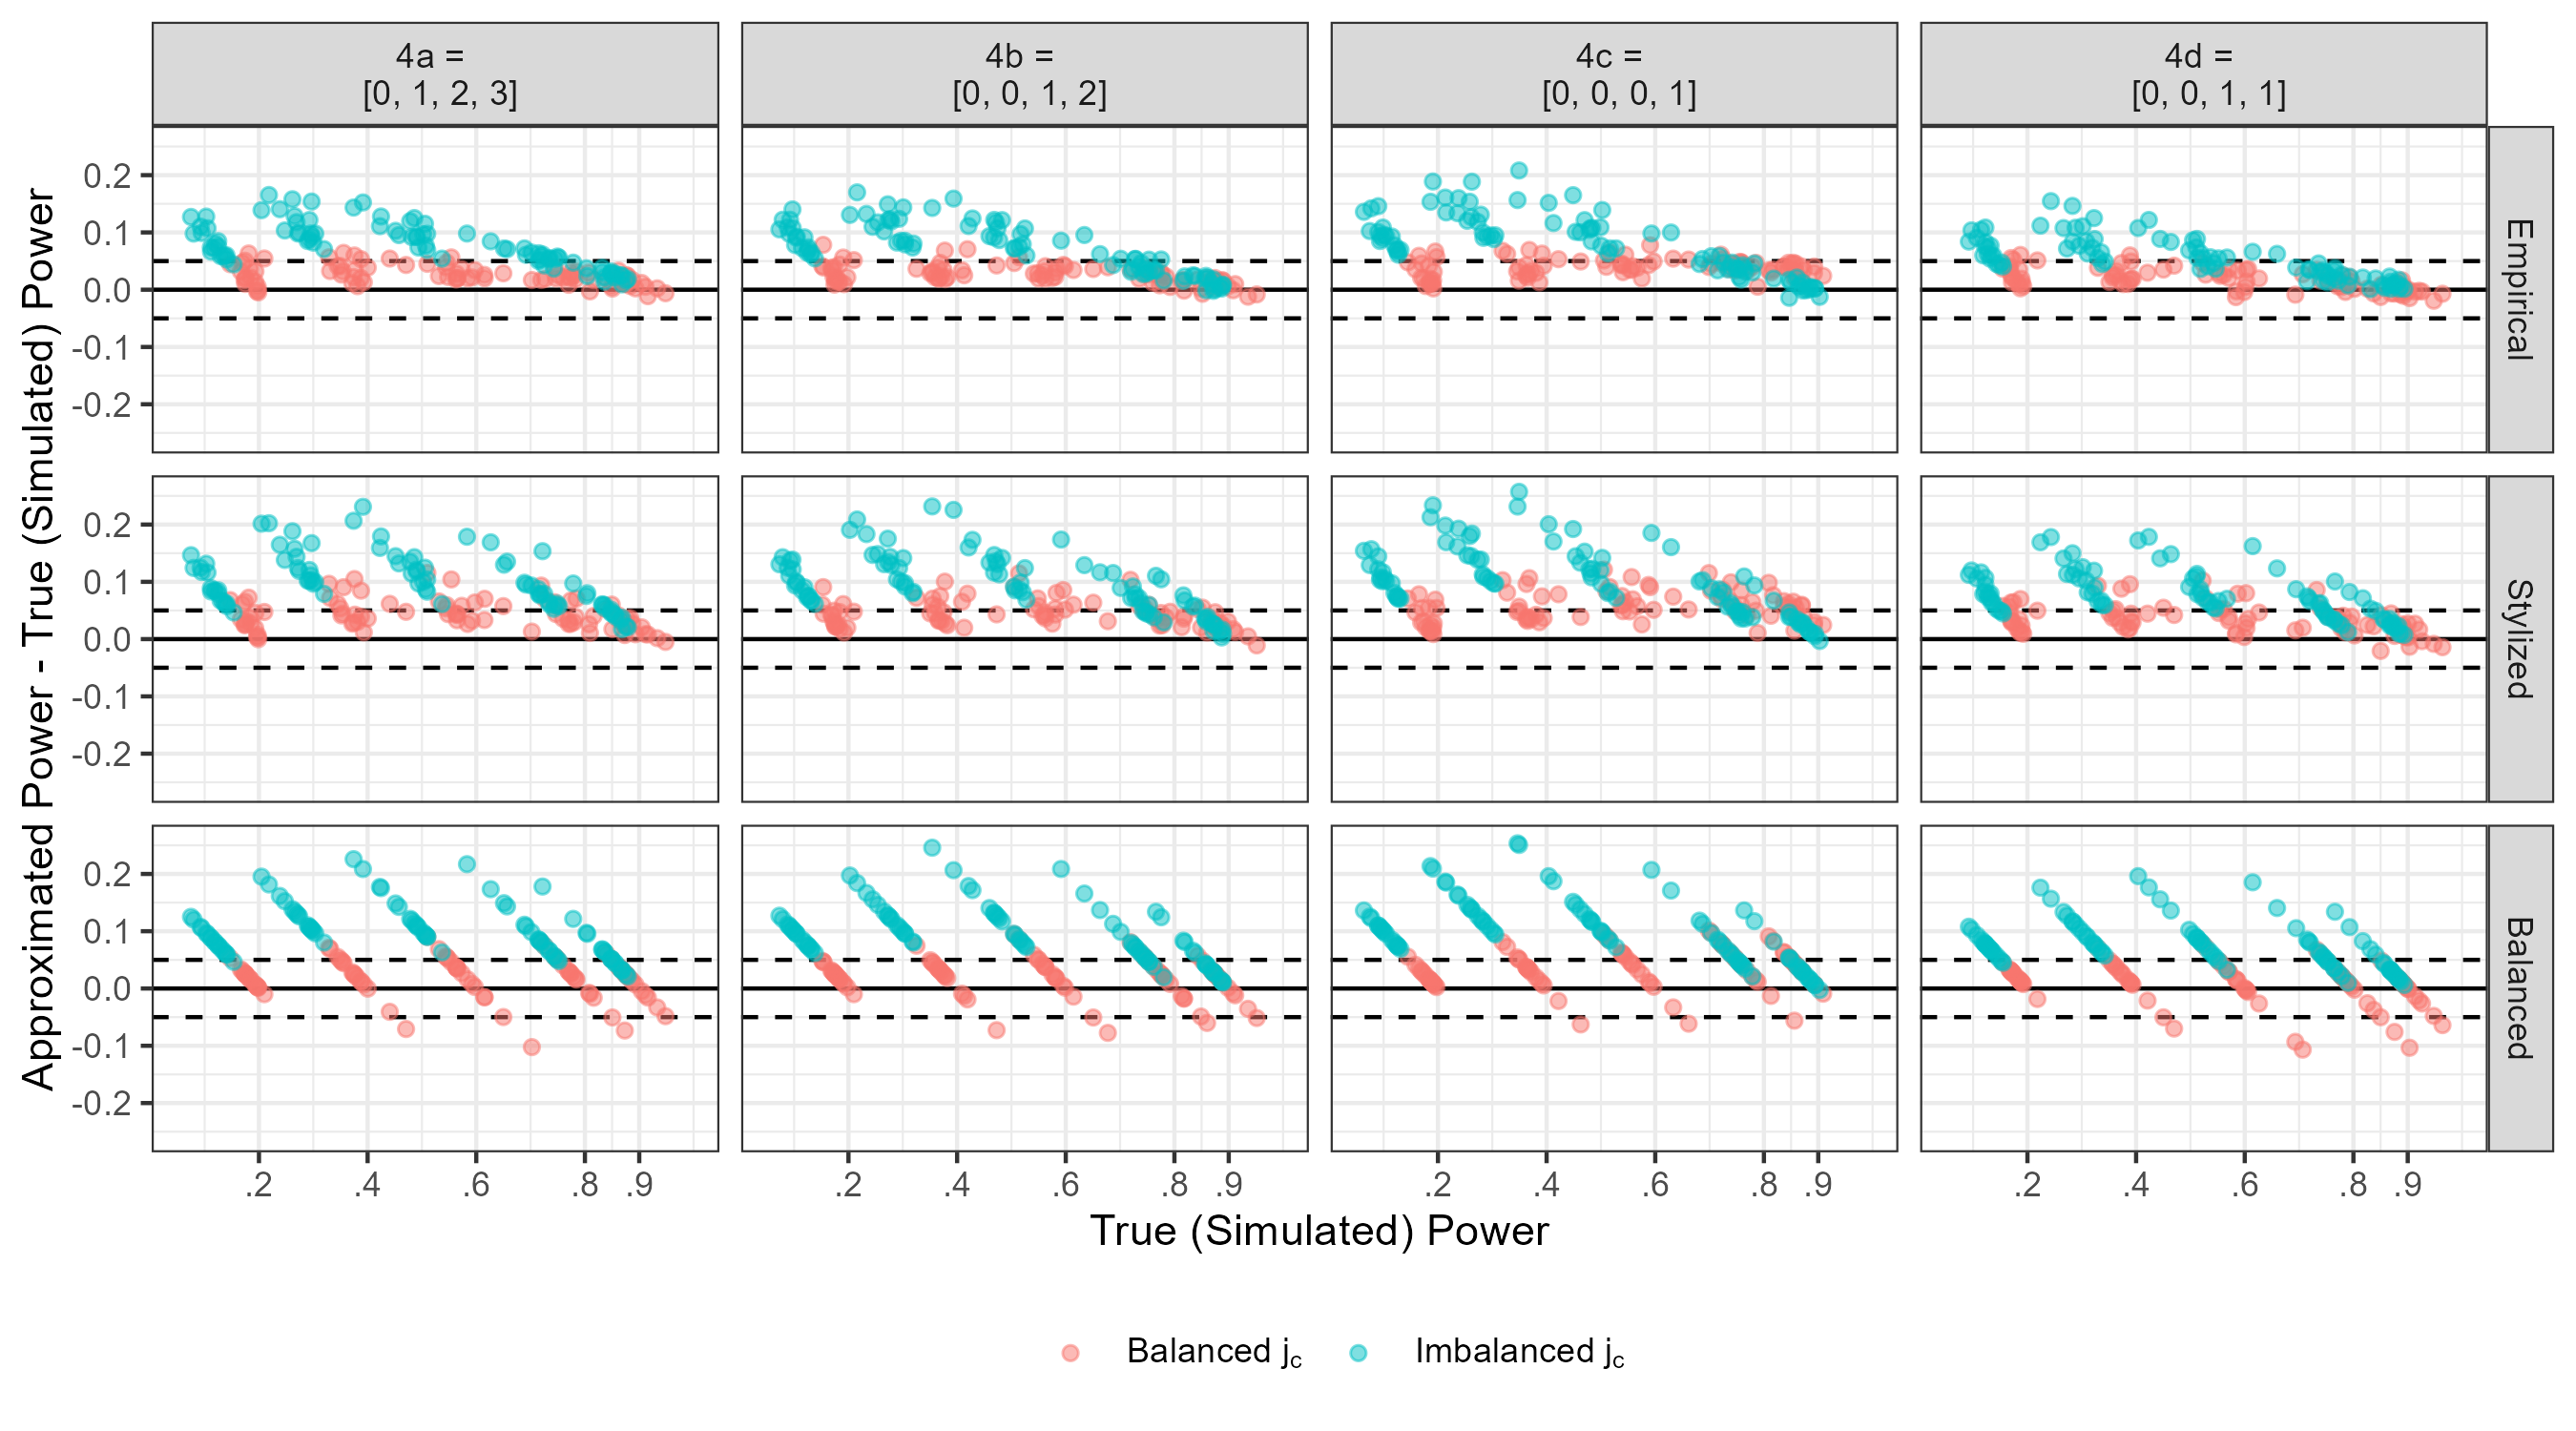
\includegraphics[width=\linewidth]{chapters/plots/fc_bal_allsamp_rejrate_J24.png}\caption{Power discrepancy between approximation power and true power vs. true power by pattern type ($f_c$), sampling/imputation methods for the primary study characteristics, and the balance of the number of studies per category (Balanced $j_c$ vs. Imbalanced $j_c$) for $J = 24$. The solid lines indicate no discrepancy between the approximated and simulated power. The dashed lines indicate that the approximated power over- or underestimated the true power by five percentage points. \label{fig: fc_bal_allsamp_rejrate_J24}}
    \vspace{-5pt}
\end{sidewaysfigure}



\begin{sidewaysfigure}
    \centering
    \vspace{-5pt}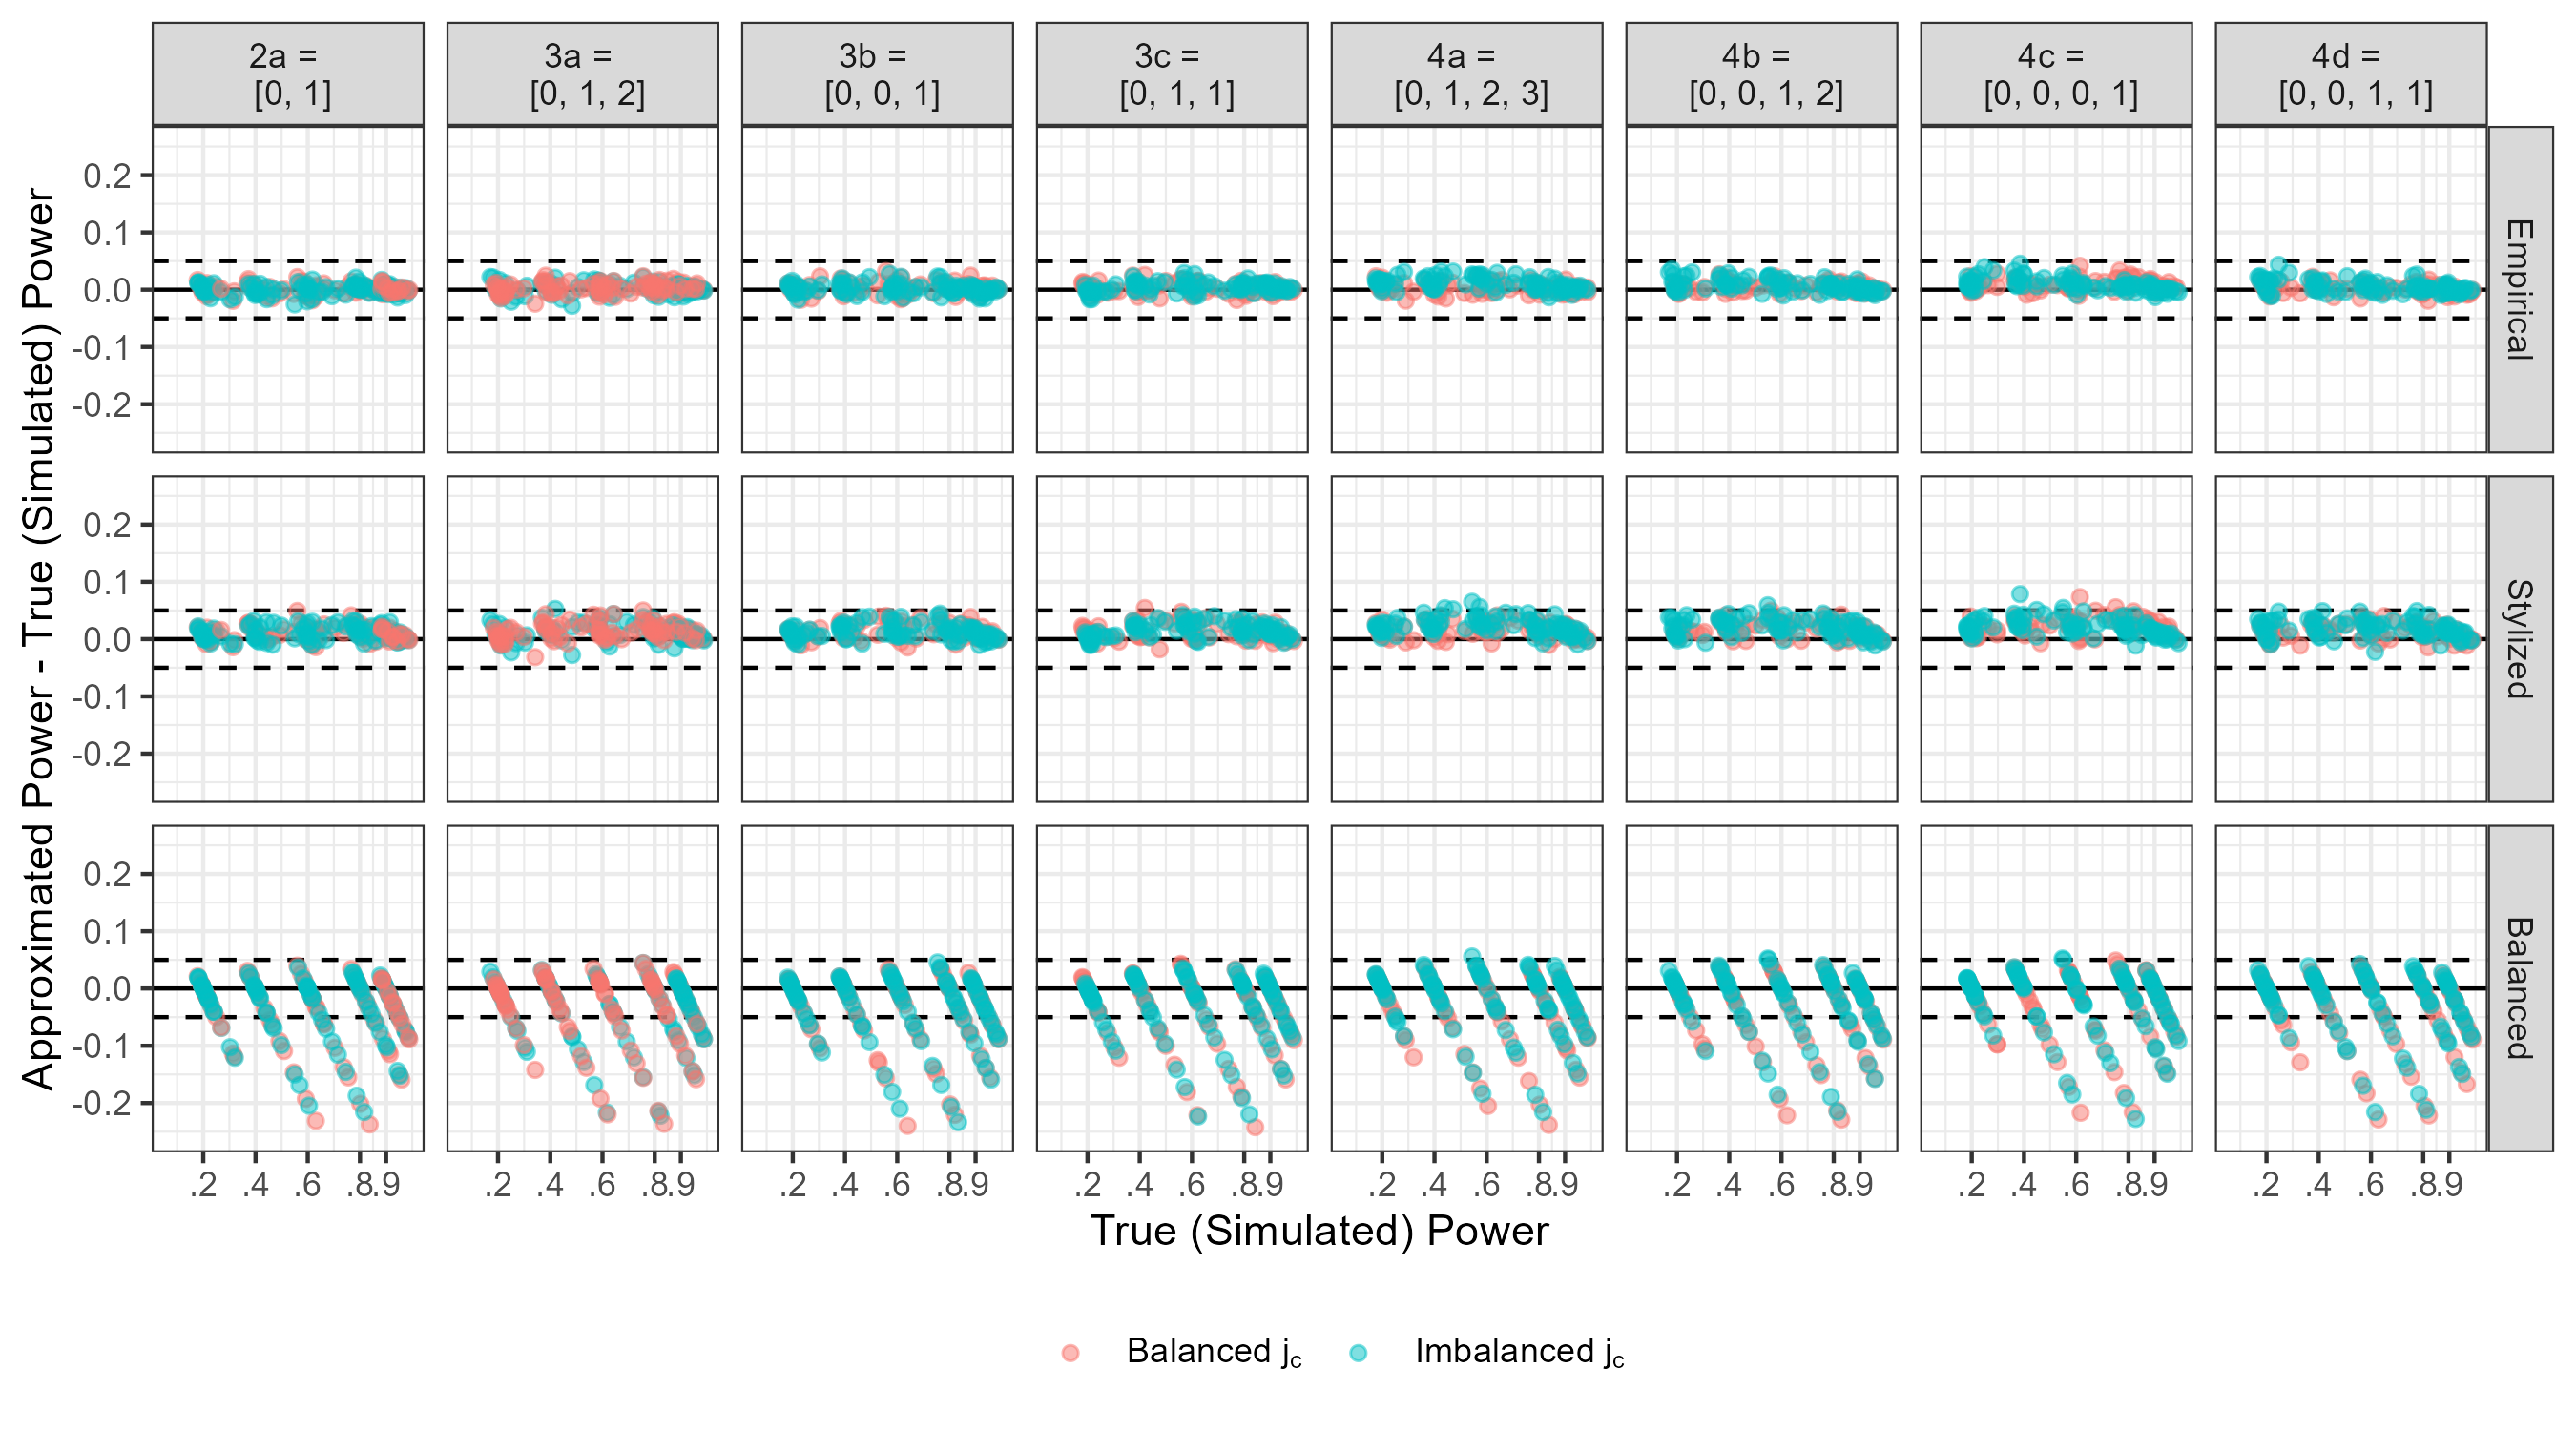
\includegraphics[width=\linewidth]{chapters/plots/allsamp_bal_J72.png}\caption{Power discrepancy between approximation power and true power vs. true power by pattern type ($f_c$), sampling/imputation methods for the primary study characteristics, and the balance of the number of studies per category (Balanced $j_c$ vs. Imbalanced $j_c$) for $J = 72$. The solid lines indicate no discrepancy between the approximated and simulated power. The dashed lines indicate that the approximated power over- or underestimated the true power by five percentage points. \label{fig: allsamp_bal_J72}}
    \vspace{-5pt}
\end{sidewaysfigure}

\begin{sidewaysfigure}
    \centering
    \vspace{-5pt}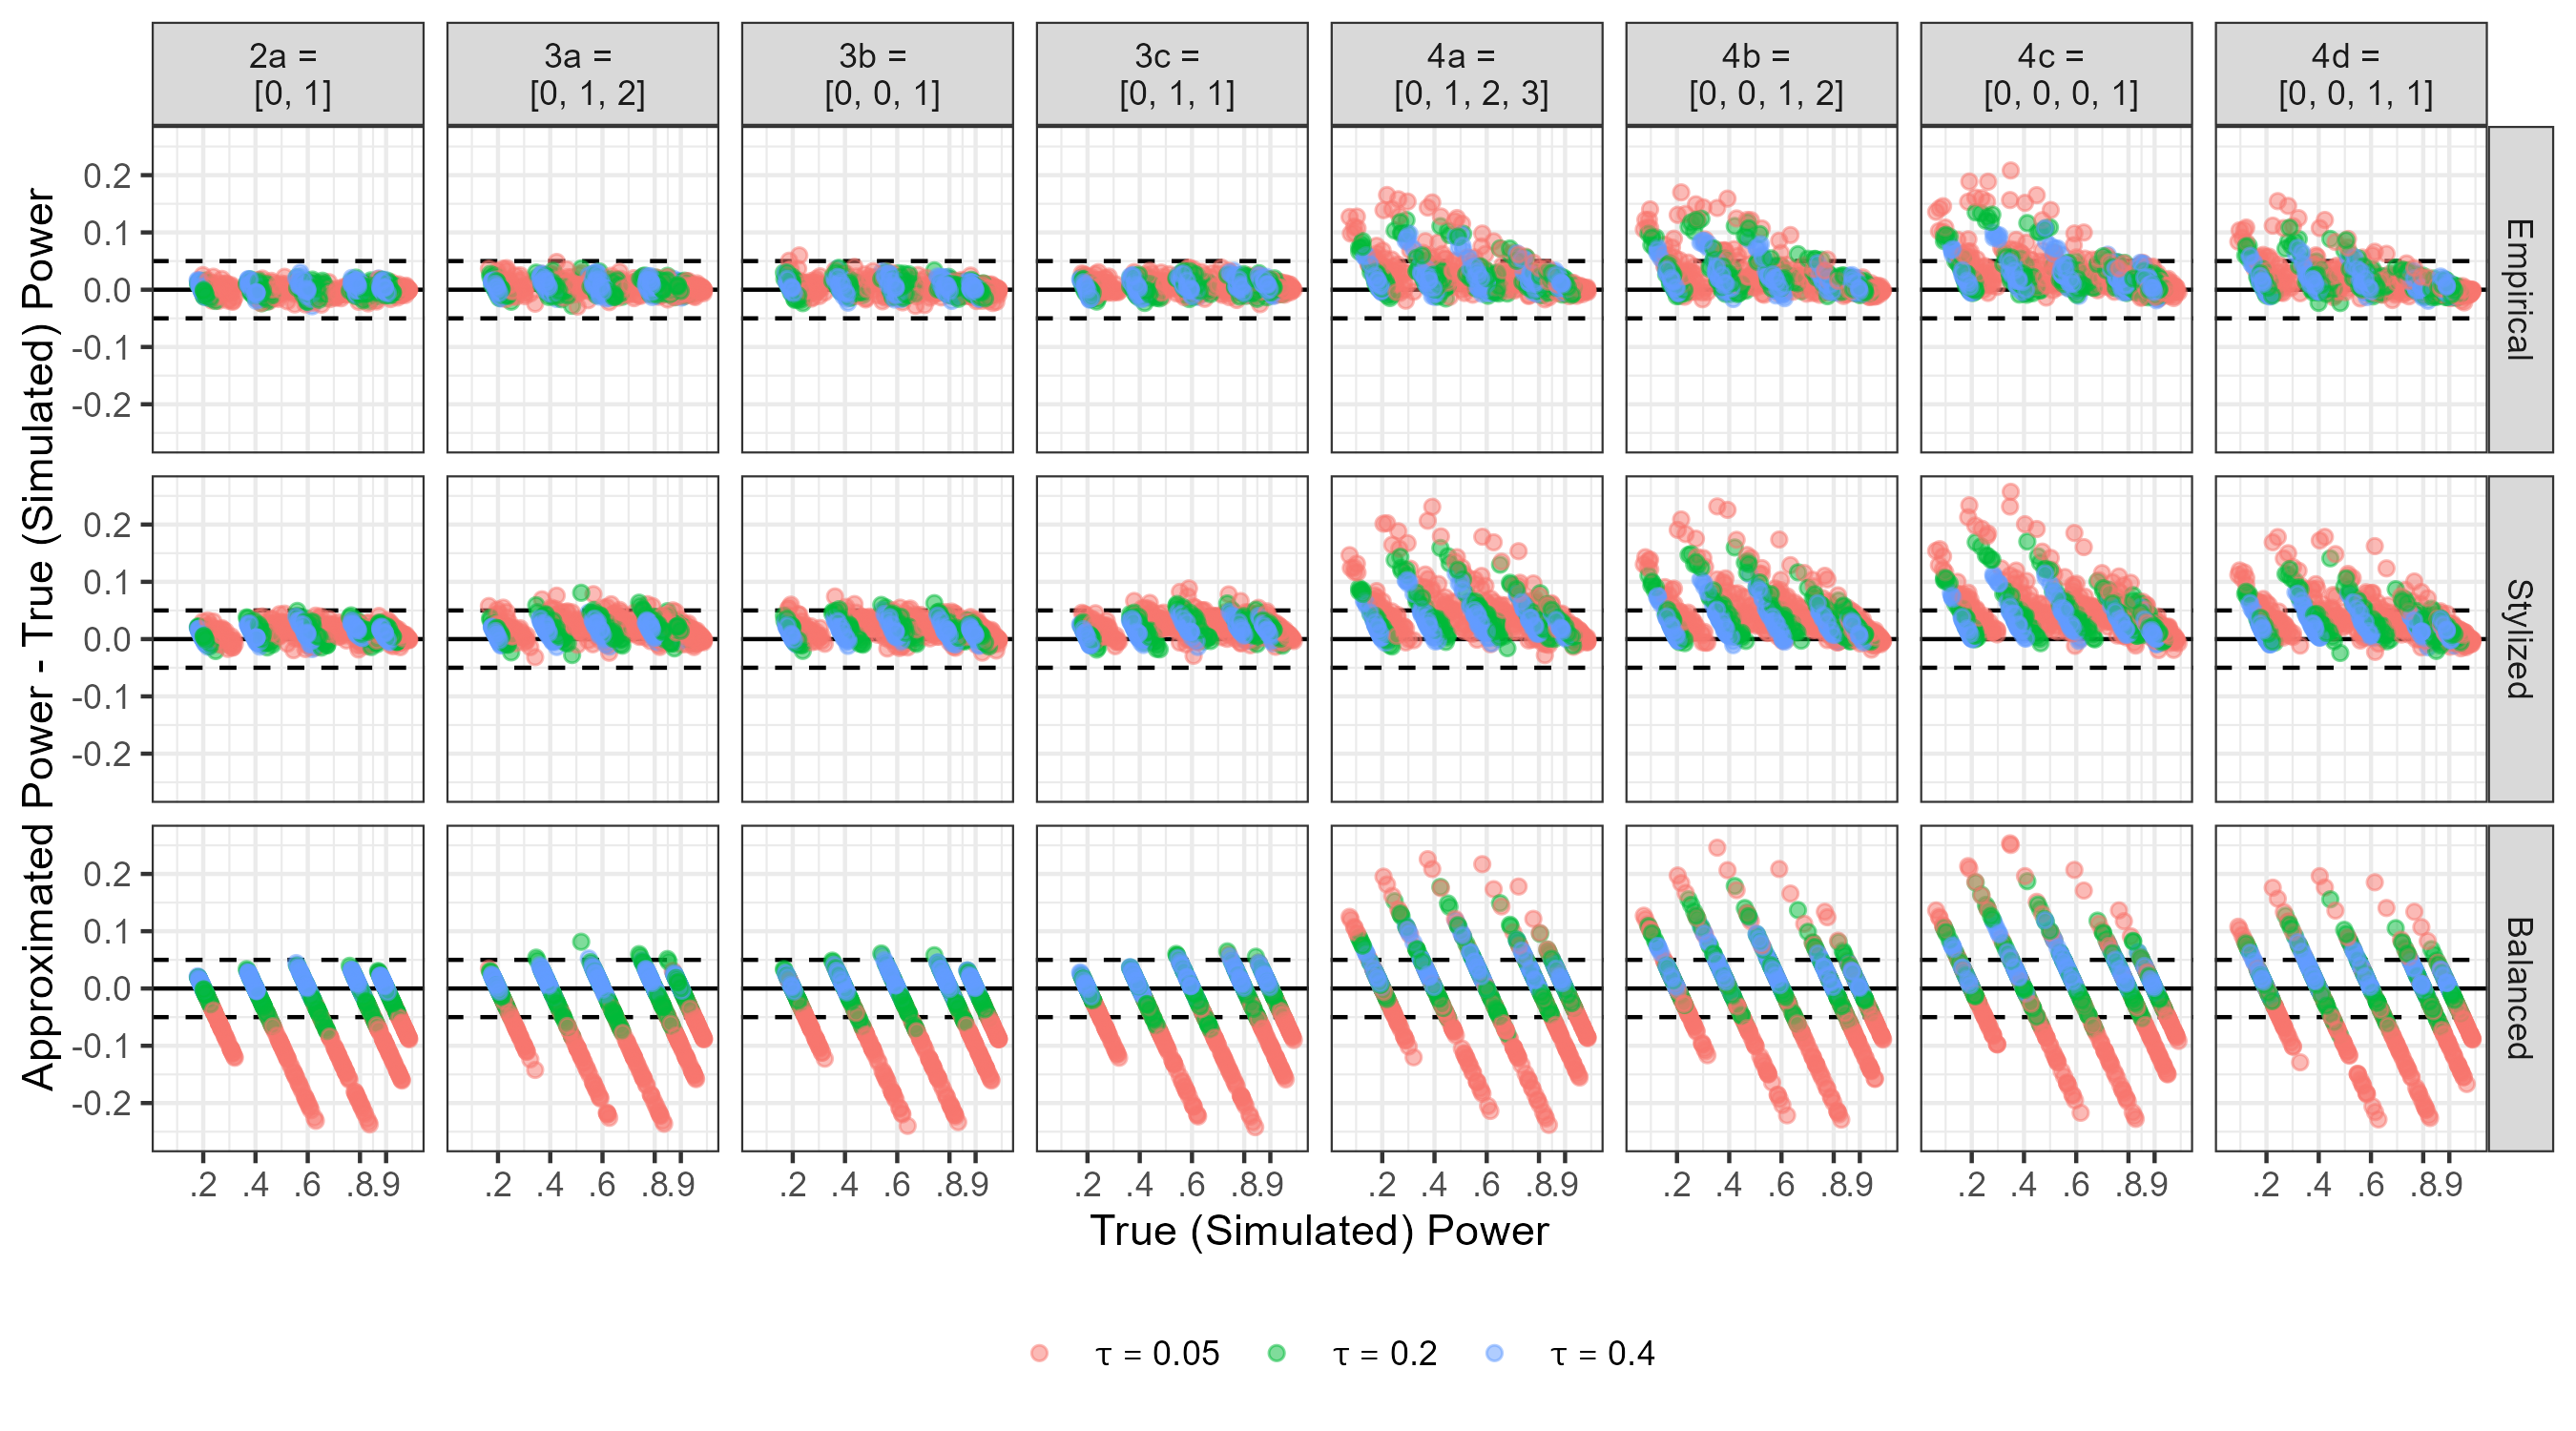
\includegraphics[width=\linewidth]{chapters/plots/allsamp_tau.png}\caption{Power discrepancy between approximation power and true power vs. true power by pattern type ($f_c$), sampling/imputation methods for the primary study characteristics, and between-study heterogeneity ($\tau$). The solid lines indicate no discrepancy between the approximated and simulated power. The dashed lines indicate that the approximated power over- or underestimated the true power by five percentage points. \label{fig: allsamp_tau}}
    \vspace{-5pt}
\end{sidewaysfigure}

Figures \ref{fig: fc_omega_all_samp_rejrate} and \ref{fig: fc_rho_all_samp_rejrate} have the within-study heterogeneity ($\omega$) and the sampling correlation ($\rho$) mapped onto color, respectively. Figures \ref{fig: fc_omega_all_samp_rejrate} and \ref{fig: fc_rho_all_samp_rejrate} show that the power discrepancies for the empirical and stylized sampling methods do not vary by the $\rho$ nor $\omega$ factors. For the balanced assumption method, Figure \ref{fig: fc_omega_all_samp_rejrate} shows that $\omega$ does explain some differences between the simulated power and the approximated power, where the balanced assumption method underestimates the true power to a greater degree when $\omega = 0.05$.  
 
\begin{sidewaysfigure}
    \centering
    \vspace{-5pt}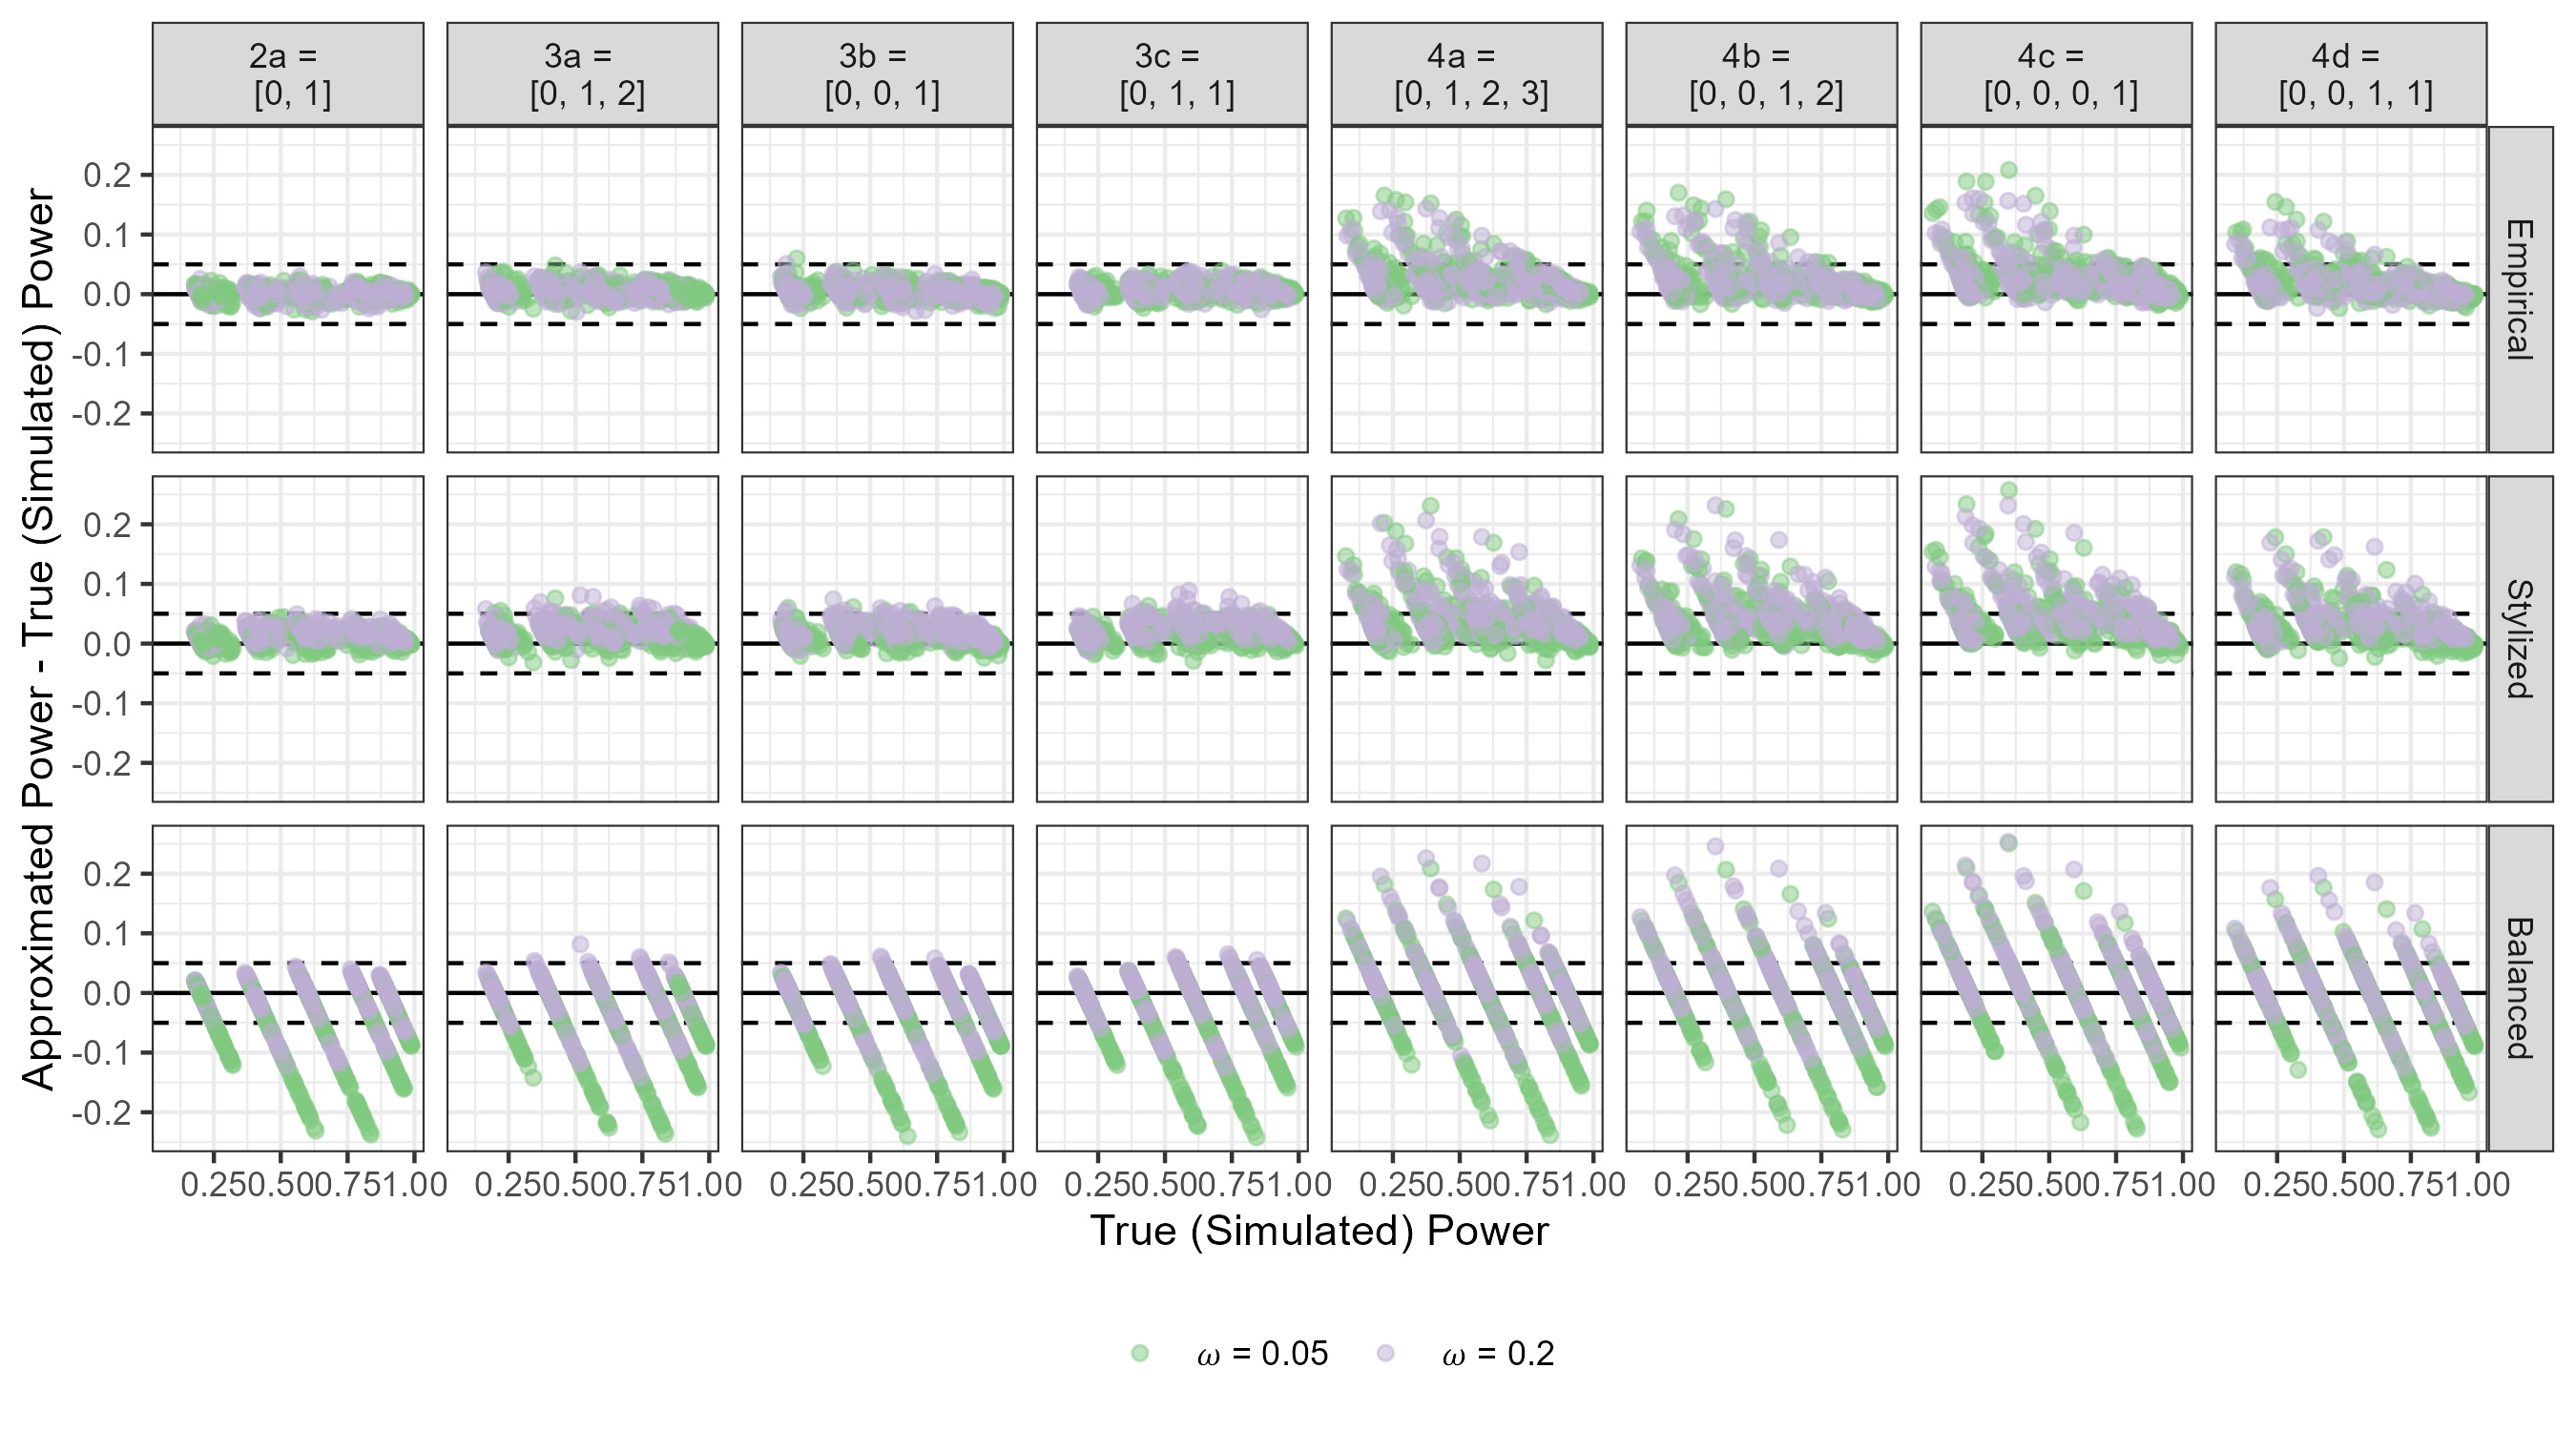
\includegraphics[width=\linewidth]{chapters/plots/fc_omega_all_samp_rejrate.png}\caption{Power discrepancy between approximation power and true power vs. true power by pattern type ($f_c$), sampling/imputation methods for the primary study characteristics, and within-study heterogeneity ($\omega$). The solid lines indicate no discrepancy between the approximated and simulated power. The dashed lines indicate that the approximated power over- or underestimated the true power by five percentage points.\label{fig: fc_omega_all_samp_rejrate}}
    \vspace{-5pt}
\end{sidewaysfigure}

\begin{sidewaysfigure}
    \centering
    \vspace{-5pt}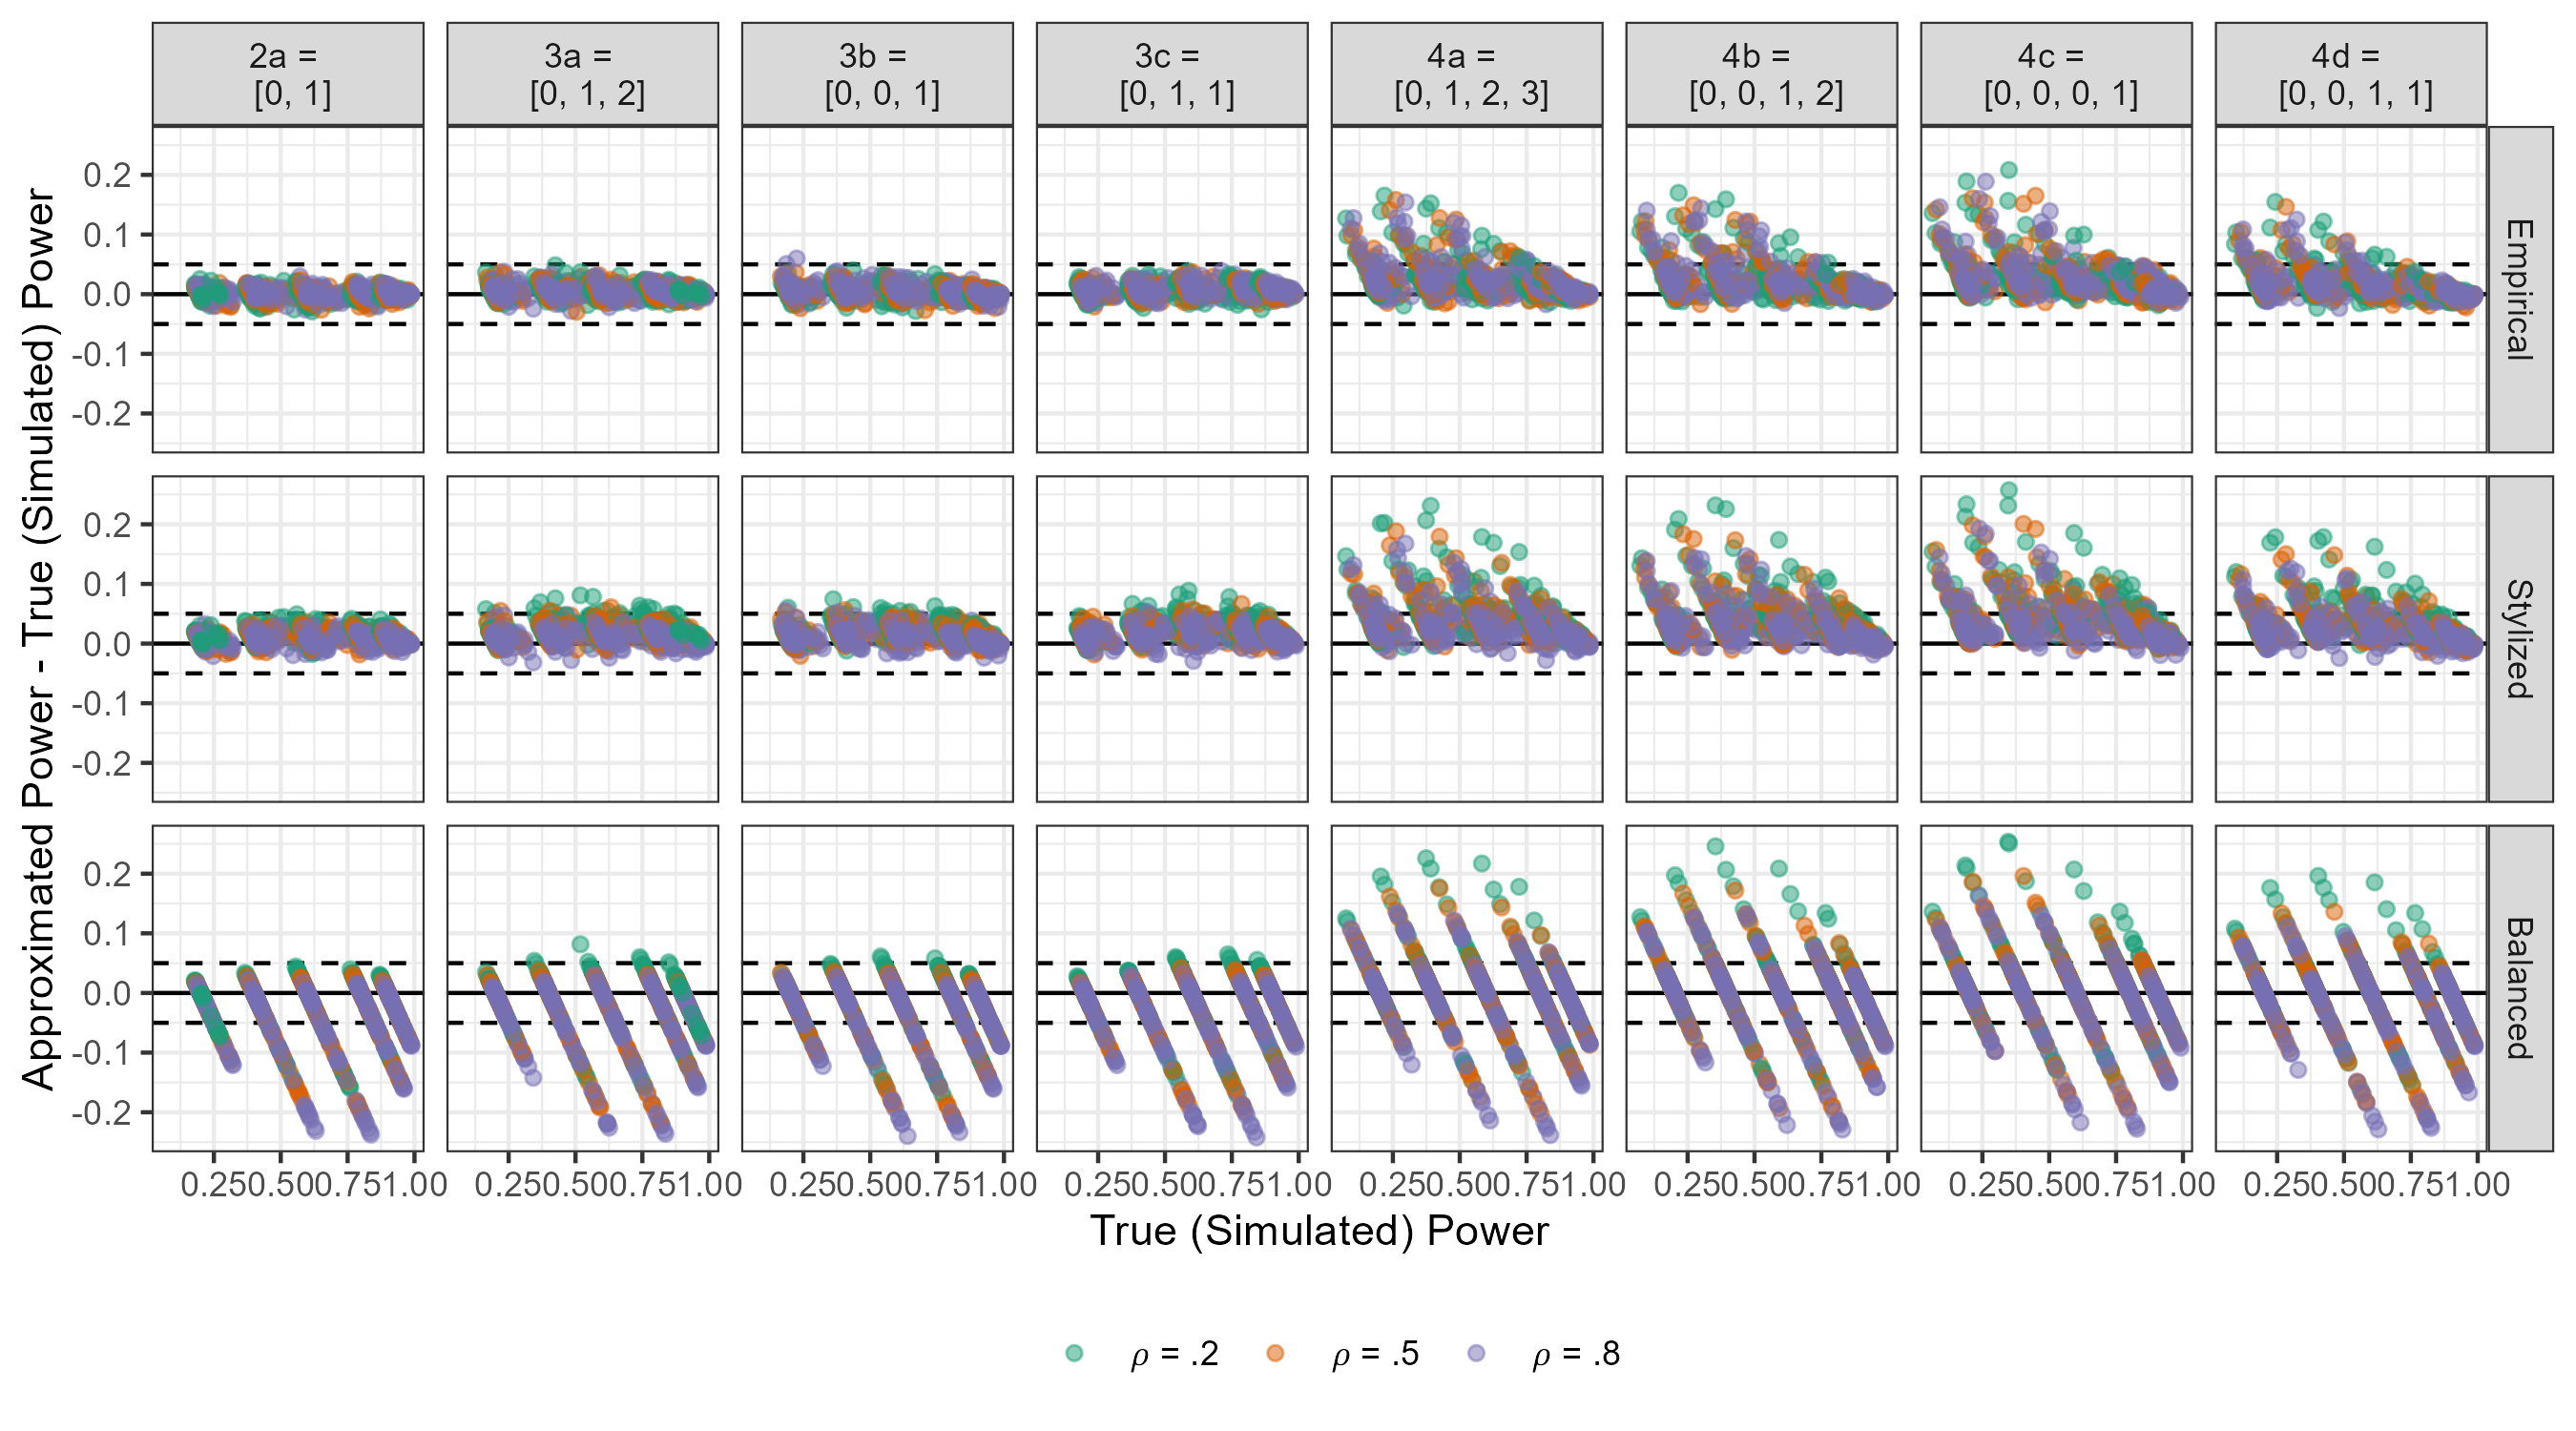
\includegraphics[width=\linewidth]{chapters/plots/fc_rho_all_samp_rejrate.png}\caption{Power discrepancy between approximation power and true power vs. true power by pattern type ($f_c$), sampling/imputation methods for the primary study characteristics, and sampling correlation ($\rho$). The solid lines indicate no discrepancy between the approximated and simulated power. The dashed lines indicate that the approximated power over- or underestimated the true power by five percentage points. \label{fig: fc_rho_all_samp_rejrate}}
    \vspace{-5pt}
\end{sidewaysfigure}

\section{Type I Error Rates}

In the following sections, I present the results of the analysis of deviance for the nominal error results and an accompanying visual analysis.

\subsection{Analysis of Deviance for Type I Error Rates}

Table \ref{tab:SequentialAnalysis - Nominal Error} presents the results of the analysis of deviance for the nominal error (please refer to Section \ref{sec: analysis of deviance} for details on the methods for this analysis). The residual deviance for the null model was $5892.6$. The following are the top ten factors and interactions based on the ranking: 1) the total number of studies ($J$), 2) the interaction between the total number of studies and the pattern of the $\mu_c$ ($J \times f_c$), 3) the pattern of the $\mu_c$ ($f_c$), 4) the between-study heterogeneity ($\tau$), 5) the balance of the number of studies across categories ($bal. j_c$),
6) the interaction between the total number of studies and the between-study heterogeneity ($J \times \tau$), 7) the interaction between the between-study heterogeneity and the pattern of the $\mu_c$ ($\tau \times f_c$), 8) the interaction between the total number of studies and the balance of the number of studies across categories ($J \times bal. j_c$), 9) the interaction between the the pattern of the $\mu$ and the balance of the number of studies across categories ($f_c \times bal. j_c$), and 10) the interaction between the between-study heterogeneity and the balance of the number of studies across categories ($\tau \times bal. j_c$). 

From this ranking, it seems that $J$, $f_c$, $bal. j_c$, and $\tau$ and their interactions explain the variation in empirical Type I error rates. Notably, $\omega$ and $\rho$ do not seem to influence the Type I error rates much. In the sections below, I describe the visual analysis results of Type I error rates, particularly focusing on the most influential factors.

\begin{table}[H]
\caption{Sequential Analysis of Deviance for Type I Error}
     \label{tab:SequentialAnalysis - Nominal Error}
    \centering
    \begin{tabular}{p{3cm}p{3cm}p{3cm}p{3cm}}
        \toprule
    Term & d.f. & Deviance & Rank \\ \midrule
       Null deviance & & 5892.6 & \\
        &&&\\
       $Deviance$ & & & \\
       $J$ & 4 & 1257.3 & 1 \\
       $\tau$ & 2 & 489.7 & 4  \\ 
       $\omega$ & 1 & 9.0 & 13 \\
       $\rho$ & 2 & 2.4 & 18 \\
       $f_c$ & 7 & 526.4 & 3 \\
       $bal. j_c$ & 1 & 340.3 & 5 \\
       $J:\tau$ & 8 & 318.8 & 6  \\ 
       $J:\omega$ & 4 & 2.7 & 17 \\
       $J:\rho$ & 8 & 7.6  & 15 \\
       $J:f_c$ & 28 & 615.8  & 2  \\
       $J:bal. j_c$ & 4 & 257.3  & 8  \\
       $\tau:\omega$ & 2 &  0.4 & 19  \\
       $\tau:\rho$ & 4 & 14.3 & 12 \\
       $\tau:f_c$ & 14 & 273.5 & 7 \\
       $\tau:bal. j_c$ & 2 & 41.5 & 10 \\
       $\omega:\rho$ & 2 & 0.1 & 20 \\
       $\omega:f_c$ & 7 & 8.5 & 14 \\
       $\omega:bal. j_c$ & 1 & 6.5 & 16 \\
       $\rho:f_c$ & 14 & 14.9 & 11 \\
       $\rho:bal. j_c$ & 2 & 0.04 & 21 \\ 
       $f_c:bal. j_c$ & 7 & 120.8 & 9 \\
        \bottomrule
    \end{tabular}
   
    \small
      d.f. = Degrees of freedom; $J$ is the total number of primary studies factor; $\tau$ is the between-study heterogeneity factor; $\omega$ is the within-study factor; $\rho$ is the sample correlation factor; $f_c$ is the pattern of the $\mu_c$ factor; $bal. j_c$ is the balance of the $j_c$ factor. 
   % \caption{Caption}
\end{table}

\subsection{Type I Error Rates}

I was also interested in evaluating the Type I error rates for the CR2 variance estimator and the HTZ degrees of freedom with the CHE model. I found that the Type I error rate of the HTZ test did not exceed the nominal level across all conditions; however, it was below the nominal error rate, especially with more categories, a small number of total studies, an imbalanced number of studies per category, and small between-study heterogeneity. 

%Figures \ref{fig: type1error_bal}, \ref{fig: type1error_omega}, \ref{fig: type1error_rho}, \ref{fig: type1error_tau}, and \ref{fig: type1error_bal_tau} display boxplots of the Type I error rates across the design factors. 

Figures \ref{fig: type1error_bal} and \ref{fig: type1error_bal_tau} display boxplots of the Type I error rates across the design factors. The solid lines represent the nominal error, and the dashed line is the boundary for the MCSE, which is equal to $\alpha + 1.96 \times MCSE_{r\alpha}$. 

In Figure \ref{fig: type1error_bal}, the pattern of the $\mu_c$ ($f_c$) is the y-axis, the Type I error rate is the x-axis, the number of total studies ($J$) and the balance of the number of studies per category (Balanced $j_c$ vs. Imbalanced $j_c$) are mapped on to the facets. Figure \ref{fig: type1error_bal} shows that the cluster-robust Wald test results in Type I error rates below the nominal level when there are more categories. This is particularly true when $J = 24$ and $J = 36$ for $C = 4$ and when $J = 24$ for $C = 3$ and there is an imbalance in the $j_c$.  The Type I error rate should ideally be at the nominal level. The balance of the $j_c$ across $C$ does result in the HTZ test being more conservative as well, with the imbalanced $j_c$ across the $C$ condition resulting in lower Type I error rates, comparatively. 

Following the results of the analysis of deviance, I also decided to evaluate the influence of between-study heterogeneity after accounting for the other impactful factors. Figure \ref{fig: type1error_bal_tau} has facets for between-study heterogeneity ($\tau$) and number of total studies ($J$), and the balance of the number of studies per category (bal. $j_c$) mapped to the color. While the boxes are rather small, the figure shows that the level of $\tau$ impacts Type I error rates as well. From this figure, the HTZ test is more conservative when $J$ is small, with a greater number of categories, and imbalanced $j_c$, but particularly when there is small between-study heterogeneity.

\begin{figure}
    \centering
    \vspace{-5pt}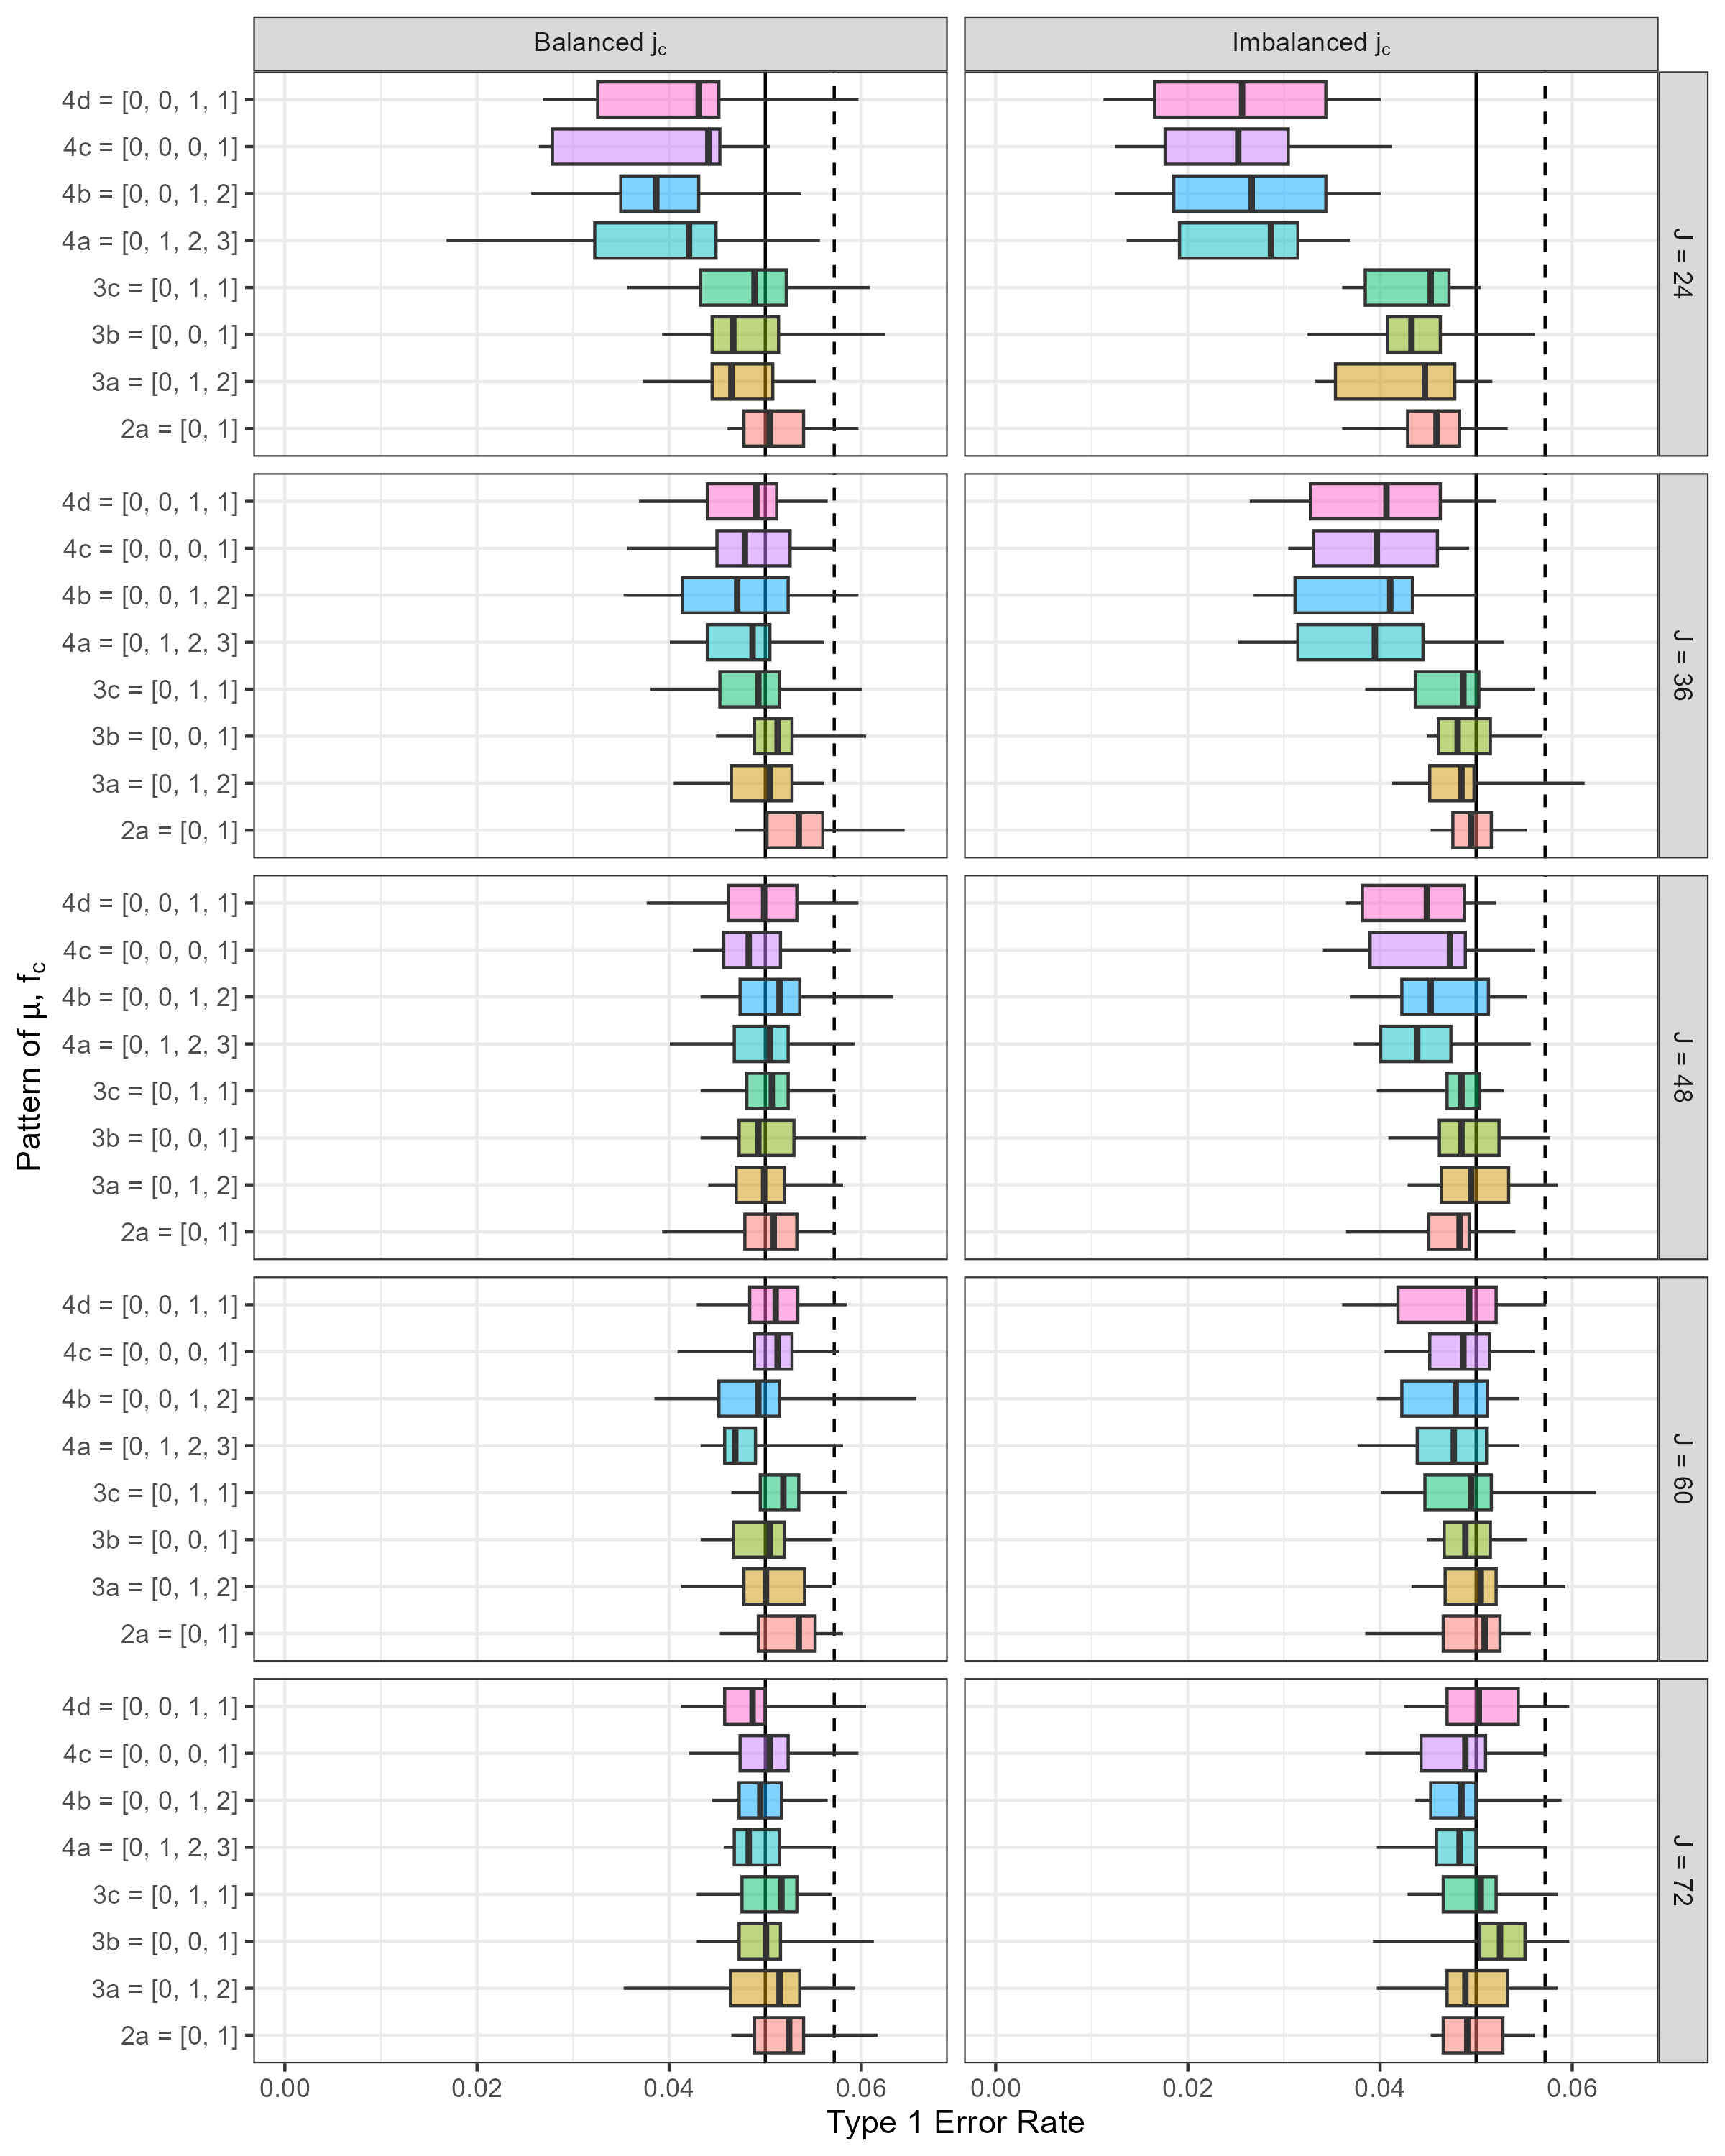
\includegraphics[width=\linewidth]{chapters/plots/type1error_bal.png}\caption{Type I error by pattern type ($f_c$), the number of studies ($J$), and the balance of the number of studies per category (Balanced $j_c$ vs. Imbalanced $j_c$). The solid lines indicate the nominal  $\alpha$ level of $.05$. The dashed lines indicate bounds for simulation error.\label{fig: type1error_bal}}
    \vspace{-5pt}
\end{figure}



\begin{figure}
    \centering
    \vspace{-5pt}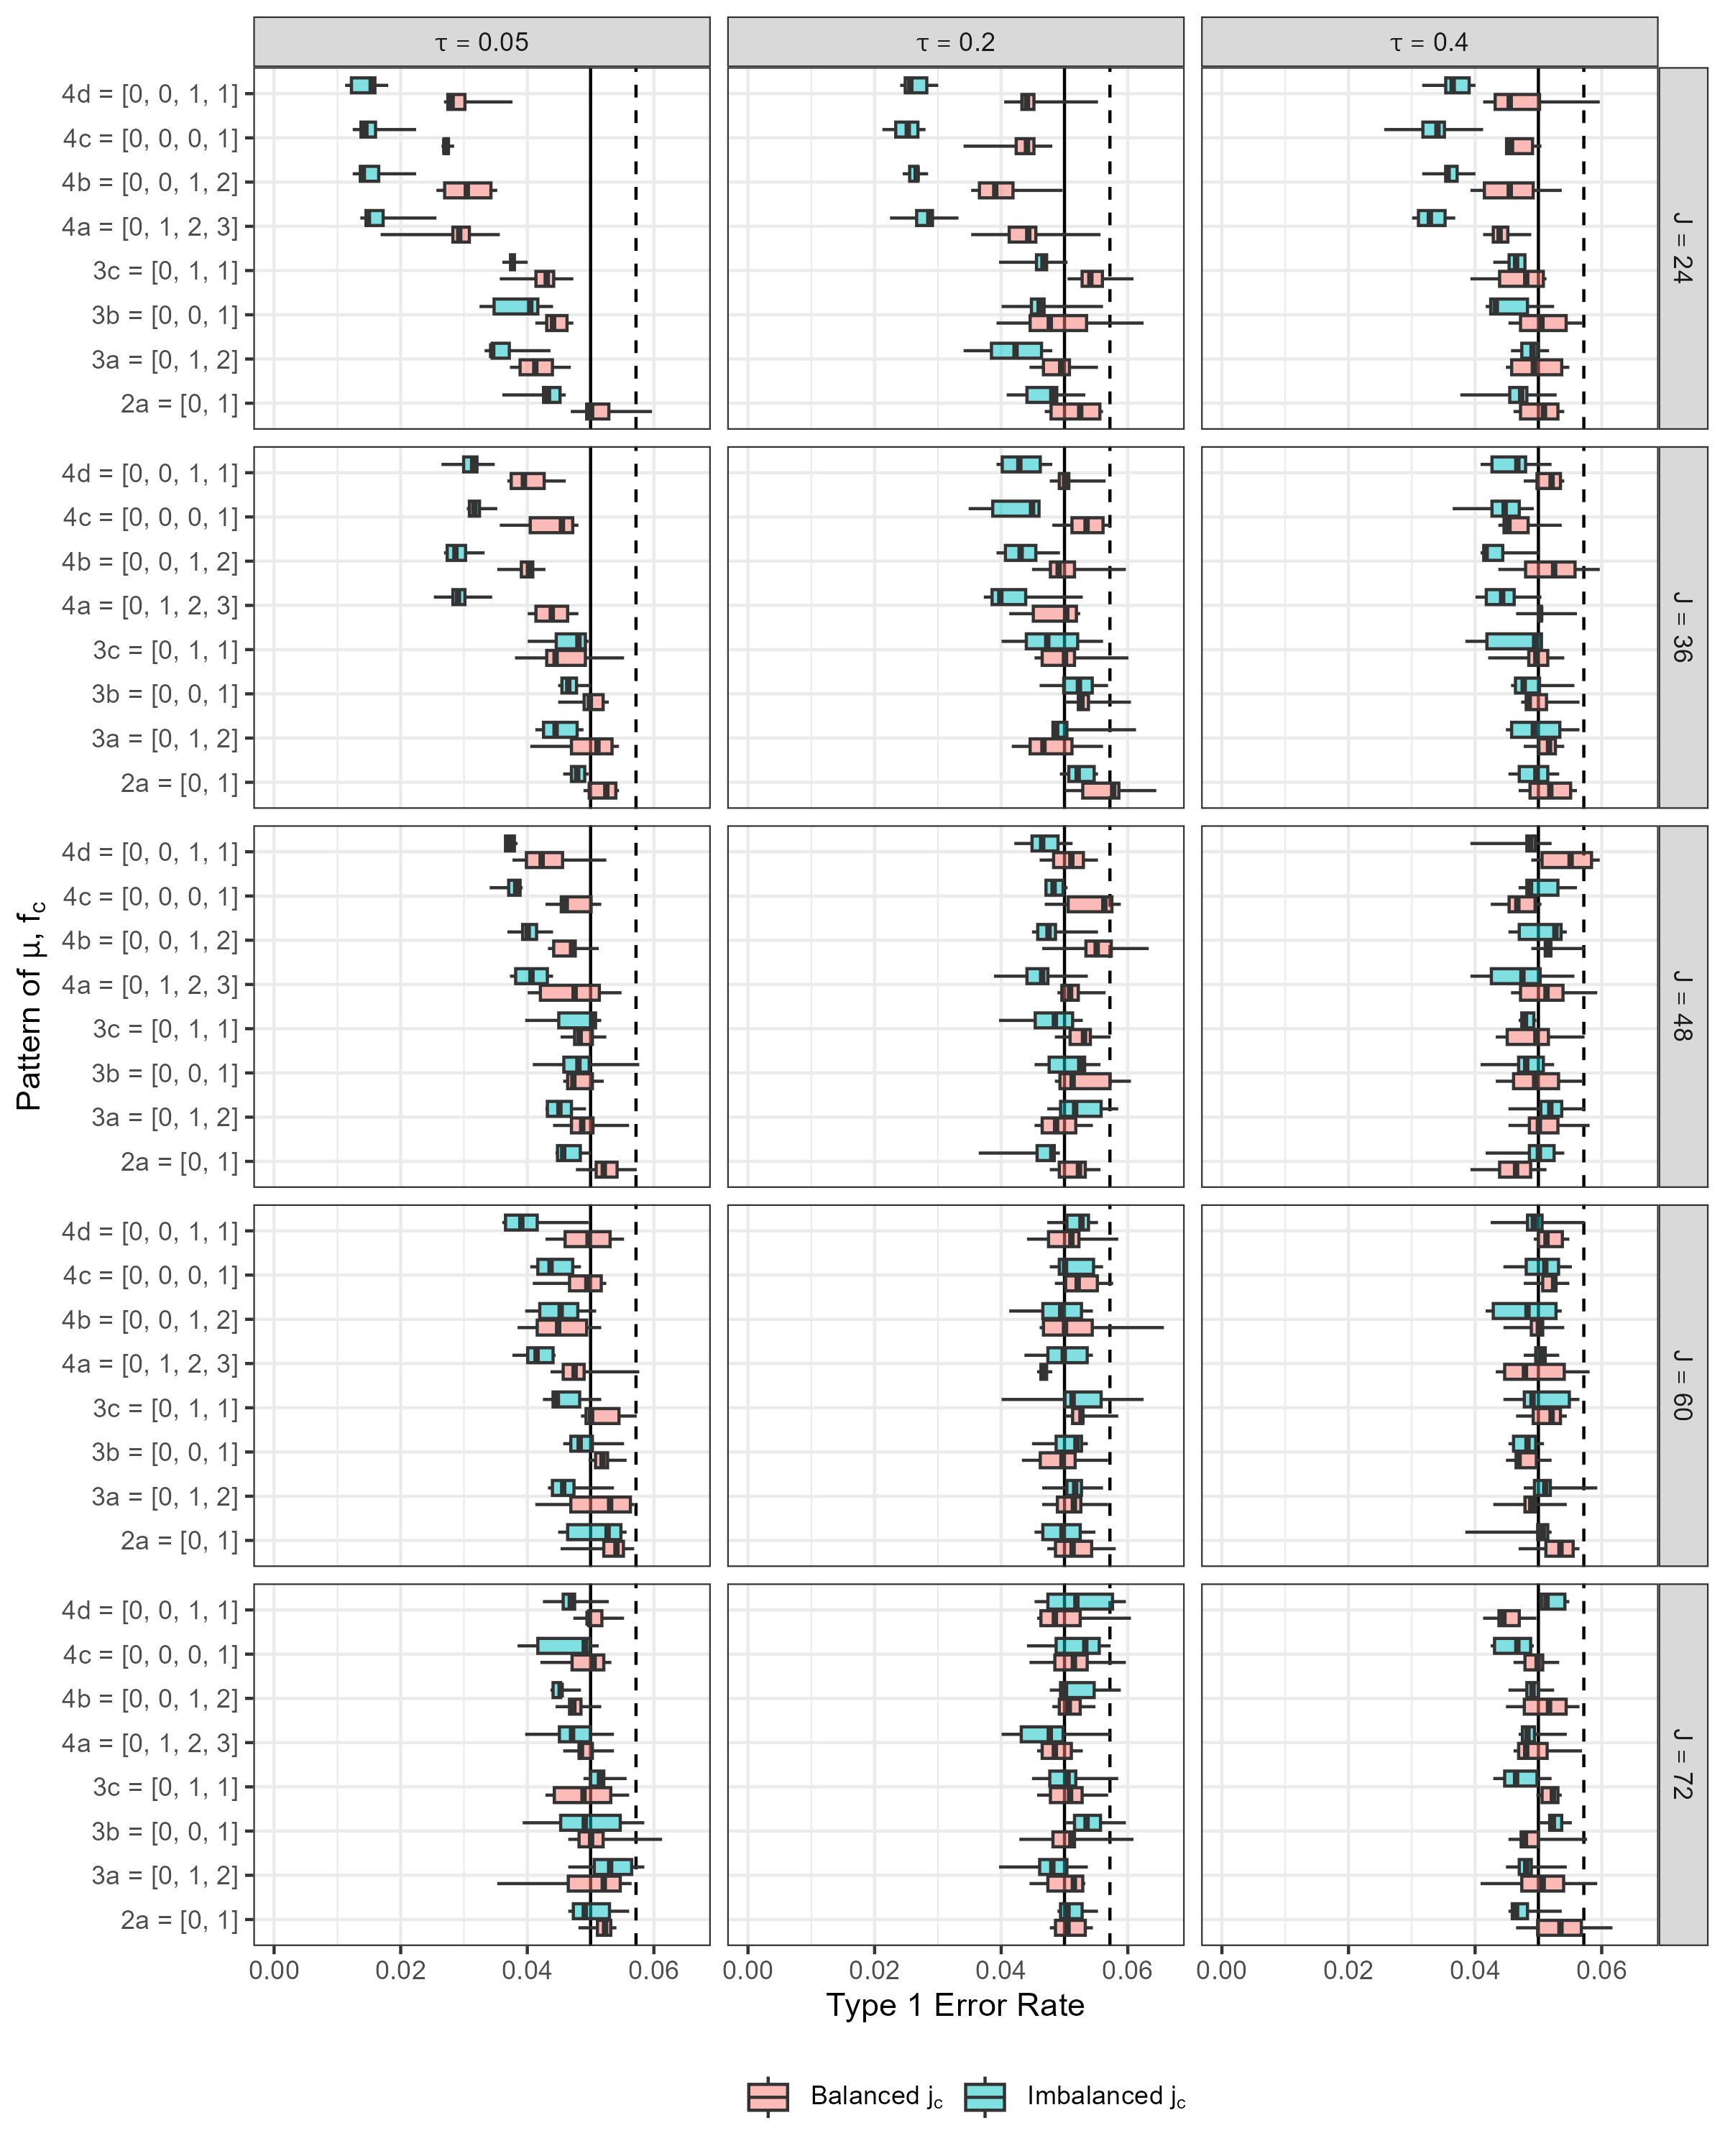
\includegraphics[width=\linewidth]{chapters/plots/type1error_bal_tau.png}\caption{Type I error by pattern type ($f_c$), the number of studies ($J$), between-study heterogeneity ($\tau$), and the balance of the number of studies per category (Balanced $j_c$ vs. Imbalanced $j_c$). The solid lines indicate the nominal $\alpha$ level of $.05$. The dashed lines indicate bounds for simulation error. \label{fig: type1error_bal_tau}}
    \vspace{-5pt}
\end{figure}








\chapter{Discussion}\label{ch: discussion}

In meta-analysis, multiple dependent effect size estimates in primary studies are prevalent, and methods that account for the dependence are widely used \autocite{hedges2010, pustejovsky2022, vandennoortgate2013, vandennoortgate2015, betsy_jane_becker_model}. A primary goal of meta-analysis is to explain heterogeneity of effect sizes through meta-regression. One way to do this is to include categorical moderators, a common type of covariate in social science meta-analytic research \autocite{tipton2019a}. With the development and wide use of working models that account for more than one source of dependence to be used with RVE meta-regression \autocite{pustejovsky2022}, a methodology for conducting power analysis for the tests of such models is needed for obtaining \textit{a priori} power estimates. Due to the complexity of these models, a larger number of studies is needed than for models for independent effect sizes, so it is important to consider performance of these models when planning a systematic review. Furthermore, using univariate \textit{a priori} power analysis methods \autocite{hedges2001} for a meta-analysis involving dependent effect sizes results in inaccurate power estimates \autocite{vembye2023}.  

\textcite{vembye2023} developed and evaluated approximation formulas for the power of the test of the overall pooled effect for the MLMA, CE, and CHE working models. I extended this work in my dissertation by developing and evaluating a closed-form approximation for the HTZ tests of study-level categorical moderators for the CHE model.  Below, I first discuss the implications of the results I found and then I detail the limitations of this study and offer future directions. 


\section{Implications}

% the primary conclusion is that the approximation is accurate except for high number of categories and small degrees of freedom. Something that can calculated in advanced. Do power calculation in advanced and look at the degrees of freedom, if very small than maybe don't trust the result.


I had three aims for my study: 1) To validate the approximation for the power of the Wald test of a categorical study-level moderator from the CHE model with HTZ degrees of freedom through a simulation; 2) To compare methods for assuming sampling variances and the number of effect sizes in the power approximation formula; and 3) To evaluate Type I Error for the robust-Wald Test from a CHE working model. From the results of this study, I conclude that 1) The power approximation formula is accurate when there are a small number of contrasts, but it can be inaccurate in conditions with a larger number of contrasts and small degrees of freedom; 2) It is important to find reliable pilot data for sampling the number of the effect sizes and the sampling variances, as the accuracy of the formula did depended on how closely the assumed distributions matched the data generating distributions; and 3) The Type I Error of the robust-Wald Test from a CHE working model was below the nominal error rate, especially in conditions with more contrasts and a small number of total studies. I expand on these conclusions below.  

For the first aim, under an ideal situation where the primary study characteristics for the power approximation were sampled from the same dataset used to generate the simulated data, the results showed that the power estimates of the approximation formula are accurate for the true power of the robust-Wald test for the CHE model when there were a smaller number of categories ($C \leq 3$) and in cases where there were a larger number of categories ($C = 4$) and large datasets ($J \geq 60$). However, under some conditions, when there were more categories and a small to moderate total number of studies ($J \leq 48$), the approximation formula overestimated the true power by as much as $20.81$ percentage points. Furthermore, the balance of the number of studies across categories and the between-study heterogeneity impacted the magnitude of the power discrepancy, with imbalance in the number of studies across categories and smaller between-study heterogeneity resulting in the biggest power discrepancies. The approximation never underestimated true power. 

%Under the conditions I evaluated and the sampling techniques for the $k_j$ and $\sigma_j^2$, the approximation never underestimated the true power. Furthermore, across all conditions except for a few when $C=4$, the approximation power estimates were within the threshold of $5\%$ of the true power. However, I did not assess the mis-specification of these values. 

One possible reason that the approximation overestimated the true power could be related to the findings of my third aim, where I found that the simulated Type I error rates for the cluster-robust Wald test of the study-level categorical moderator are conservative when the number of contrasts ($q$) is greater and when the total number of studies was small. These findings are consistent with those of \textcite{tipton2015b} and \textcite{joshi_cluster_2022}; they also found that while none of the factors yielded Type I error rates substantially above nominal levels, the HTZ test has more conservative Type I error rates and becomes even more conservative when there are more contrasts. While the HTZ test performs well at controlling Type I error, the power of the test is penalized when the number of contrasts, $q$, increases. The reason is that as $q$ increases, the multiplier of the $Q$ to equate it to an $F$ ($[(\eta_z - q +1)/(\eta_zq)]$) and the denominator degrees of freedom of the $F$-statistic ($d_2 = \eta_z - q +1$) decrease \autocite{tipton2015b}. 

While this conservatism in the Type I error rate lowers the likelihood of making a Type I error, its source could also lower statistical power. The low power is attributable to the test being conservative, which could be why the approximation overstates the power. Perhaps the power of a more appropriately calibrated method for the Wald test, like the cluster wild bootstrap test (CWB) examined by \textcite{joshi_cluster_2022}, may be more aligned with the power estimates of the approximation.  
\textcite{joshi_cluster_2022} examined CWB as an alternative small-sample correction test to the HTZ test, and they found that CWB controls for Type I error and provides more power than the HTZ test, especially for tests of multiple contrasts. A future study validating the proposed approximation for the power of the CWB test is worth conducting, because the CWB is computationally intensive and it would be useful to be able to estimate power for a proposed analysis that involves CWB. 



In my results, I also found that the magnitude of the degrees of freedom is a useful diagnostic indicator for whether power approximations are accurate for the HTZ Wald test, where a small degrees of freedom and more contrasts could indicate that the power approximation will overestimate the true power and a researcher should then be more cautious about the associated power estimate (see Figure \ref{fig: df_mean}). However, if the number of contrasts is smaller ($q \leq 2$) or if the number of contrasts is greater ($q \geq 3$) and there is a larger degrees of freedom value ($d_2 \geq 12$), then the approximation will be reliable. When conducting an \textit{a priori} power analysis, a meta-analyst can look at the degrees of freedom to determine whether they can trust the results. Although it is important to note that a small degree of freedom does not guarantee a large discrepancy between actual and estimated power estimates. There were a large number of samples that had small degrees of freedom due to an imbalanced number of studies across categories, small between-study heterogeneity, four categories, and/or a small total number of studies, where the approximation was accurate. Additionally, the balance of the number of studies across categories and between-study heterogeneity also impacted the magnitude of the degrees of freedom. \textcite{tipton2015b} found that degrees of freedom in a meta-regression using HTZ were smaller for imbalanced covariates as well. Finally, if there is an interest in finding the power of the HTZ test for a larger number of contrasts and a smaller number of studies, then it may be necessary instead to simulate the power of the test as I did for this study. 



Regarding the findings of my third aim independently, I was able to replicate the findings of \textcite{joshi_cluster_2022} and \textcite{tipton2015b} through a distinctly different way of simulating the design matrices and vector of $\beta$ meta-regression coefficients. Both studies used different covariate specifications that were more limited in scope. The design matrix that \textcite{tipton2015b} used in their simulation study had five covariates of various types, including one binary study-level moderator with extreme imbalance in the number of studies across the categories. They evaluated a different number of contrasts, which resulted in 26 unique coefficient vectors. In their first study, \textcite{joshi_cluster_2022} evaluated the HTZ test with the same design matrix as \textcite{tipton2015b} and 11 unique coefficient vectors. For their second study, \textcite{joshi_cluster_2022} generated a single categorical covariate as I did, but its value varied either at the study-level or effect-size level. The categorical covariate had either 3, 4, or 5 categories. For the $\beta$ coefficients, they fixed the intercept to 0.3 and varied only the first slope with three values, which resulted in 24 unique coefficient vectors. For my study, the design matrices only included study-level categorical moderators, and I induced imbalance in the number of studies across the categories through fixed proportions depending on the number of categories. Also, by generating the $\mu_c$ values through data-generating conditions, I evaluated $7,203$ unique coefficient vectors (See Figure \ref{fig:max_mu} for the maximum $\beta$ estimate value of each coefficient vector). I was also able to replicate the findings of \textcite{joshi_cluster_2022} and \textcite{tipton2015b} using a different working model than they used in their simulation studies.  \textcite{joshi_cluster_2022} used a correlated effects working model where \textcite{tipton2015b} used a fixed effects working model. I replicated their findings under a wider range of design matrices, regression coefficients, and a more general working model.   

%Other factors that impacted the degree to which the HTZ test was below the nominal error rate were the balance of the number of studies per category and the magnitude of between-heterogeneity. 


%% really can't rely on stylized in all conditions. It was always off. Similar pattern. max 2-3 % off from empirical in the conditions.  

For the conclusions of my second aim, I found that the approximate power estimates that result from sampling within-study characteristics from a stylized distribution followed the same pattern as those that result from sampling within-study characteristics from an empirical distribution. Neither sampling method performed well when $C=4$, and there was a small to moderate number of studies. However, the empirical sampling method performed slightly better with a maximum overestimation of $20.82$ percentage points compared to that of the stylized method's $25.72$ percentage point overestimation. Also, when the number of contrasts was small, the stylized method did overestimate the true power by more than five percentage points in some conditions ($C = 3$ and $J \leq 36$) by as much as $8.85$ percentage points. As \textcite{vembye2023} noted, since reliable pilot data is not always available for an \textit{a priori} power analysis, meta-analysts can use stylized distributions of $k_j$ and $\sigma_j^2$ for the approximation. In practice, I suggest factoring in that the stylized sampling method will overestimate the true power more than reliable pilot data. 

For the balanced assumption method, the true power was at most $25.3$ percentage points above and $24.2$ percentage points below a power of $60\%$. Assuming that the primary study characteristics are balanced resulted in substantially underestimated power estimates for the Wald test with the CHE+RVE model across all conditions except when $C=4$, and there were a small to moderate number of studies where it also overestimated the true power. Therefore, I do not recommend that meta-analysts use the balanced method in practice. 


\section{Limitations and Future Directions}

Below, I detail limitations to this study that should be considered to determine the extent to which these results can be generalized. I also highlight areas where this study can be extended. 

The proposed approximation of the cluster-robust Wald test only applies to study-level categorical moderators. I first focused on categorical moderators because they are commonly used in meta-analytic practice \autocite{ahn2012, tipton2019}. 
Additional work is needed to develop approximations for within-study categorical and between-study and within-study continuous moderators. As \textcite{vembye2023} noted, and I also faced in this dissertation study, it is necessary to make assumptions about the distribution of the covariate across studies and effect sizes. That can be challenging in practice. In future research, the balance of the number of effect sizes and the number of studies across covariates should also be considered for within-study moderators.  
The proposed power approximation for the robust-Wald test of study-level categorical moderators was developed for data structures that follow the CHE model, while \textcite{vembye2023} developed and evaluated approximations for the CE and MLMA working models for the test of the overall pooled effect as well. For my purposes, I chose not to look at special cases of the CHE model where there is no within-study variance or no correlation among effect sizes because meta-analytic data often has both sources of dependence \autocite{pustejovsky2022}. Because it is possible for data structures to have only one type of dependence, though, it may be worthwhile to develop approximations for these special cases. Additionally, the proposed approximation should be validated when the simulated data follows a different working model (such as $\rho=0$ for the MLMA model or $\omega=0$ for the CE model).

Furthermore, this approximation only proposed HTZ-based degrees of freedom, not model-based degrees of freedom, nor other robust tests such as the Eigen-decomposition F-test or the Eigen-decomposition and transformation test \autocite{tipton2015b}. I decided to first focus on developing the HTZ-based degrees of freedom for RVE because \textcite{vembye2023} found that the approximations that used RVE were more accurate than the model-based ones, where model-based tests had inflated Type I error for the test of the overall pooled effect. Also, the model-based degrees of freedom will have close to-correct Type I error only when the working model is correctly specified \autocite{vembye2023}. For the eigen-decomposition-based methods, \textcite{tipton2015b} found that they also resulted in high Type I error rates. 

% Also, there is still the open question of how the power and Type I error of the robust Wald tests compare to the power of the model-based Wald tests. Model-based tests could have inflated Type I error, as \textcite{vembye2023} found for the test of the overall pooled effect.

Additionally, for the simulated data, I assumed that the effect sizes in each study and across studies were equally correlated, which may not accurately reflect the reality in which the sampling correlation varies across studies. Also, it could be that variability in sampling correlation impacts the power of the true estimates, and therefore, also affects the discrepancy between the true and approximated power. Future studies could generate a sampling correlation that varies between studies by assuming it follows a $Beta$ distribution as was done in \textcite{tipton2015b, joshi_cluster_2022, vembye2023}. Another next step would be to examine when the sampling correlation used in the data-generating process is different from the sampling correlation used in the estimation or the approximation formula.

For this study, I only used one empirical distribution of $k_j$ and $\sigma_j^2$ to validate the approximation. Further steps should be taken to validate the approximation with other distributions of $k_j$ and $\sigma_j^2$ to test whether the approximation results in more inaccurate power estimates.  Another limitation of this study is that the distributions of $k_j$ and $\sigma_j^2$ for the stylized sampling method were pretty similar to those of the empirical distributions. Further work is needed to evaluate how robust the approximation is to using estimates of $k_j$ and $\sigma_j^2$ drawn from a distribution quite different from that of the data-generating sample. 

Further work is needed to evaluate imputing other numbers besides the mean of the empirical distribution for the balanced method for assuming values for $\sigma_j^2$ an $k_j$ in the approximation. Alternatives include using the harmonic mean of $\sigma_j^2$, which will lead to somewhat larger studies overall, or computing the weights for an entire empirical distribution given the design characteristics $\tau^2$, $\omega^2$, and $\rho$ and imputing the average of the weights. 

The conclusions of this study are limited to the study design conditions examined (Table \ref{tab:experimentalconditions}). For example, the smallest value for the total number of studies factor that I evaluated was $24$. Still, many applied researchers have meta-analytic datasets with an even smaller total number of studies. Furthermore, I only looked at a maximum of four categories when a categorical moderator could have many more categories in practice. Also, because there are infinite possibilities, specifying alternative hypotheses for multiple contrasts can be challenging. The patterns of the $\mu_c$ were my first attempt to specify possible alternative hypotheses, but this can be refined in future studies. I believe a review of meta-analyses on the number of categories, the number of studies per category, and the distribution of regression slopes is needed to create more design conditions to test this approximation. 

%Furthermore, applied meta-analysts often encounter missing data in moderators across primary studies, decreasing the meta-analysis's power. Future studies can look at ways to account for missing data in the power approximation. 

I simulated standardized mean differences, so given distributional similarities, these results likely can also be applied to Fisher-Z transformed correlation effect sizes. Still, the results will not translate to other effect size types like odds ratio without further assumptions \autocite{vembye2023}.

Finally, further work is needed to develop guidelines for conducting a power analysis using this approximation, as was done in \textcite{vembye2024}. Also, to make the approximation more accessible, it should be implemented in an R software package such as \texttt{POMADE} \autocite{POMADE}.


\section{Conclusions}

An \textit{a priori} power analysis helps meta-analysts and potential funders determine whether a number of studies is large enough to detect an effect size of practical importance. Additionally, \textit{a priori} power analysis helps in planning a confirmatory research project when developing the analytic methodology. Applied researchers could conduct a power analysis for a meta-regression through a Monte Carlo simulation. However, such an analysis is not always accessible and takes time to develop. Having the approximation formula available makes the \textit{a priori} power analysis more straightforward.










% NOTE: If you have only one appendix, use the command \appendix instead
% of \appendices.
%
% \appendix
%%%%%%or %%%%
\appendices


\chapter{Derivations Related to the Test of the Overall Pooled Effect Size for one category} \label{App: overallpooled}

In order to be able to find the derivation of the HTZ Approximation for the Robust Variance Estimator of a study-level categorical predictor, I will need to have the derivation of the Satterthwaite degrees of freedom for the overall pooled effect size for one category. The following is the derivation that I reworked in the context of the overall pooled effect size for each category that follows the derivation from \textcite{vembye2023} for the overall pooled effect size that can be found in Supplementary S2.2 of that paper. To be able to do this, I parameterized the meta-regression model as a no-intercept model so that each category is a separate intercept and amounts to the overall pooled effect for that specific category, $\overline{\bm{T}}_c$

Let $\overline{\bm{T}}_c = (\overline{T}_{1c}, \overline{T}_{2c}, ..., \overline{T}_{Jc})$ be the $Jc \times 1$ vector of average effect sizes from each study within a category. Let $\bm{W}_c = diag(\tilde{w}_{1c}, \tilde{w}_{2c}, ..., \tilde{w}_{Jc})$ be the $Jc \times 1$ diagonal matrix with the inverse variance weights of the CHE model along the diagonal,  let $\bm{I}_c$ be a $Jc \times Jc$ identity matrix, and let $\bm{1}_c$ be a $Jc \times 1$ vector of 1's. Assuming a CHE working model, $\overline{\bm{T}}_c \sim N(\mu \bm{1}_c, \bm{W}_c^{-1})$.   $W_c$ is the sum of the weights within a category, $W_c = \sum_{j=1}^{Jc} \tilde{w}_{jc}$. The variance components, $\hat{\omega}^2$ and $\hat{\tau}^2$, are the within and between-study variances, respectively. $\rho$ is the true sampling correlation.




%%%%%%%%%%%%%%%%%%%%%%%%%%%%%%%%%%%%%%%%%%%%%%%%%%%%%%%%%%%%%%%%%%%%%%%%%%%%%%%%%%%%%%%%%%%%%%%%%%%%%%%%%%%%%%%%%%%%%%%%%%%%%%%

\subsection{Satterthwaite Approximation for the Robust Variance Estimator}

Below, I rewrite $V^R_c $ in the form we need it to find the $ E(V^R_c)$ and $Var(V^R_c)$.
\begin{equation}
    \begin{split}
        V^R_c & = \frac{1}{W_c^2}  \sum_{j=1}^{Jc} \left[ \frac{\tilde{w}_{jc}^2 (\overline{T}_{jc} - \hat{\mu_c})^2}{1-\frac{\tilde{w}_{jc}}{W_c}} \right] \\
        & =  \frac{1}{W_c^2}  \sum_{j=1}^{Jc} \left[ \tilde{w}_{jc}^2 (\overline{T}_{jc} - \hat{\mu_c})^2 \left(1-\frac{\tilde{w}_{jc}}{W_c}\right)^{-1}  \right] \\
        & =  \frac{1}{W_c^2}  \sum_{j=1}^{Jc} \left[ \tilde{w}_{jc}^2 \left(\overline{T}_{jc} - \frac{1}{W_c}\sum_{j=1}^{Jc} \tilde{w}_{jc}\overline{T}_{jc}\right)^2 \left(1-\frac{\tilde{w}_{jc}}{W_c}\right)^{-1}  \right] \\
        & =  \frac{1}{W_c^2}  \sum_{j=1}^{Jc} \left[ \tilde{w}_{jc}^2 \left(\overline{T}_{jc} - \frac{\overline{T}_{jc} \tilde{w}_{jc}}{W_c}\right)^2 \left(1-\frac{\tilde{w}_{jc}}{W_c}\right)^{-1}  \right] \\
        & =  \frac{1}{W_c^2}  \sum_{j=1}^{Jc} \left[ \tilde{w}_{jc}^2 \left( \overline{T}_{jc}^2 \left(1- \frac{\tilde{w}_{jc}}{W_c}\right)^2 \right) \left(1-\frac{\tilde{w}_{jc}}{W_c}\right)^{-1}  \right] \\
    \end{split}
    \nonumber
\end{equation}
Then in order to rewrite $V^R_c$ in quadradic form, let:
\begin{equation}
   R = \left(\mathbf{I}_c - \frac{1}{W_c} \mathbf{W_c} \mathbf{1}_c\mathbf{1}_c' \right) \mathbf{W_c} \left(\mathbf{I}_c - \frac{1}{W_c} \mathbf{W_c} \right)^{-1} \mathbf{W_c} \left(\mathbf{I}_c - \frac{1}{W_c}  \mathbf{1}_c\mathbf{1}_c' \mathbf{W_c}\right).
   \nonumber
\end{equation}
Then, $V^R_c = \frac{1}{W_c^2} \overline{T}_c'R\overline{T}_c$ when written in quadratic form. 

The mean and variance of $V^R_c$ can be obtained using properties of quadratic forms for normal random variables (Mathai \& Provost, 1992):
\begin{equation}
    \begin{split}
        E(V^R_c) & = \frac{1}{W_c^2}tr(\mathbf{R}\mathbf{W_c}^{-1}) \\
        Var(V^R_c) & = \frac{2}{W^4_c} tr(\mathbf{R}\mathbf{W_c}^{-1}\mathbf{R}\mathbf{W_c}^{-1})
    \end{split}
    \nonumber
\end{equation}

Below is the proof for $E(V^R_c)$. It is important to note that  $\left(\mathbf{I}_c - \frac{1}{W_c} \mathbf{W_c} \mathbf{1}_c\mathbf{1}_c' \right)$ is idempotent. 
\begin{equation}
    \begin{split}
       E(V^R_c) & = \frac{1}{W^2_c } tr(\mathbf{R}\mathbf{W_c}^{-1}) \\
       & = \frac{1}{W^2_c} tr\left( \left(\mathbf{I}_c - \frac{1}{W_c} \mathbf{W_c} \mathbf{1}_c\mathbf{1}_c' \right) \mathbf{W_c} \left(\mathbf{I}_c - \frac{1}{W_c} \mathbf{W_c} \right)^{-1} \mathbf{W_c} \left(\mathbf{I}_c - \frac{1}{W_c}  \mathbf{1}_c\mathbf{1}_c' \mathbf{W_c}\right) \mathbf{W_c}^{-1}  \right) \\
        & = \frac{1}{W^2_c} tr\left( \left(\mathbf{I}_c - \frac{1}{W_c} \mathbf{W_c} \right)^{-1} \mathbf{W_c}   \left(\mathbf{I}_c - \frac{1}{W_c}  \mathbf{1}_c\mathbf{1}_c' \mathbf{W_c}\right) \mathbf{W_c}^{-1}  \left(\mathbf{I}_c - \frac{1}{W_c} \mathbf{W_c} \mathbf{1}_c\mathbf{1}_c' \right)  \mathbf{W_c} \right) \\
        & = \frac{1}{W^2_c} tr\left( \left(\mathbf{I}_c - \frac{1}{W_c} \mathbf{W_c} \right)^{-1}    \left(\mathbf{W_c} - \frac{1}{W_c} \mathbf{W_c}  \mathbf{1}_c\mathbf{1}_c' \mathbf{W_c}\right) \mathbf{W_c}^{-1}  \left(\mathbf{I}_c - \frac{1}{W_c} \mathbf{W_c} \mathbf{1}_c\mathbf{1}_c' \right)  \mathbf{W_c} \right) \\
        & = \frac{1}{W_c^2} tr\left( \left(\mathbf{I}_c - \frac{1}{W_c} \mathbf{W_c} \right)^{-1}    \left(\mathbf{W_c}\mathbf{W_c}^{-1} - \frac{1}{W_c} \mathbf{W_c}  \mathbf{1}_c\mathbf{1}_c' \mathbf{W_c} \mathbf{W_c}^{-1}\right)   \left(\mathbf{I}_c - \frac{1}{W_c} \mathbf{W_c} \mathbf{1}_c\mathbf{1}_c' \right)  \mathbf{W_c} \right) \\
        & = \frac{1}{W^2_c} tr\left( \left(\mathbf{I}_c - \frac{1}{W_c} \mathbf{W_c} \right)^{-1}    \left(\mathbf{I}_c - \frac{1}{W_c} \mathbf{W_c}  \mathbf{1}_c\mathbf{1}_c'\right)   \left(\mathbf{I}_c - \frac{1}{W_c} \mathbf{W_c} \mathbf{1}_c\mathbf{1}_c' \right)  \mathbf{W_c} \right) \\
        & = \frac{1}{W_c^2} tr\left( \left(\mathbf{I}_c - \frac{1}{W_c} \mathbf{W_c} \right)^{-1}    \left(\mathbf{I}_c - \frac{1}{W_c} \mathbf{W_c}  \mathbf{1}_c\mathbf{1}_c'\right)    \mathbf{W_c} \right) \\
        & = \frac{1}{W^2_c} tr\left( \left(\mathbf{I}_c - \frac{1}{W_c} \mathbf{W_c} \right)^{-1}    \left(\mathbf{W_c} - \frac{1}{W_c} \mathbf{W_c}  \mathbf{1}_c\mathbf{1}_c'\mathbf{W_c}\right)     \right) \\
        & = \frac{1}{W^2_c} tr\left( \left(\mathbf{I}_c - \frac{1}{W_c} \mathbf{W_c} \right)^{-1}   \mathbf{W_c} \left(\mathbf{I}_c - \frac{1}{W_c}   \mathbf{1}_c\mathbf{1}_c'\mathbf{W_c}\right)     \right) \\
         & = \frac{1}{W^2_c} tr\left( \left(\mathbf{I}_c - \frac{1}{W_c} \mathbf{W_c} \right)^{-1}   \mathbf{W_c} \left(\mathbf{I}_c -    \mathbf{1}_c\mathbf{1}_c'\frac{\mathbf{W_c}}{W_c}\right)     \right) \\
    \end{split}
    \nonumber
\end{equation}
Below are the matrices within the trace rewritten in matrix form below to make it easier to follow the derivation: 
\begin{equation}
    \begin{split}
        & = \begin{bmatrix}
            \frac{W_c}{W_c-\tilde{w}_{1c}} & 0 & \dots & 0 \\
            & \ddots & & \\
            & & &  \frac{W_c}{W_c-\tilde{w}_{jc} } 
        \end{bmatrix} \begin{bmatrix}
            \tilde{w}_{1c} & & \\
            & \ddots & \\
            & & \tilde{w}_{jc}
        \end{bmatrix} \begin{bmatrix}
            1- \frac{\tilde{w}_{1c} }{W_c} & \frac{\tilde{w}_{1c} }{W_c} & \dots   \\
            &  \ddots &  & \\
            & & 1- \frac{\tilde{w}_{jc} }{W_c} 
        \end{bmatrix} \\
        & = \begin{bmatrix}
            \frac{W_c\tilde{w}_{1c} }{W_c-\tilde{w}_{1c} } &  & \dots & \\
            & \ddots & & \\
            & & &  \frac{W_c \tilde{w}_{jc} }{W_c-\tilde{w}_{jc} } 
        \end{bmatrix}  \begin{bmatrix}
            1- \frac{\tilde{w}_{1c} }{W_c} & \frac{\tilde{w}_{1c} }{W_c} & \dots   \\
            &  \ddots &  & \\
            & & 1- \frac{\tilde{w}_{jc} }{W_c} 
        \end{bmatrix} \\
         & = \begin{bmatrix}
            \left(\frac{W_c\tilde{w}_{1c} }{W_c-\tilde{w}_{1c} }\right)\left(\frac{W_c-\tilde{w}_{1c} }{W_c}\right) &  & \dots & \\
            & \ddots & & \\
            & & &  \left(\frac{W_c\tilde{w}_{jc} }{W_c-\tilde{w}_{jc} }\right)\left(\frac{W_c-\tilde{w}_{jc} }{W_c}\right) 
        \end{bmatrix}   \\
        & = \begin{bmatrix}
            \tilde{w}_{1c} & & \\
            & \ddots & \\
            & & \tilde{w}_{jc}
        \end{bmatrix}  
    \end{split}
    \nonumber
\end{equation}
Finally, now that I have simplified the part within the trace I found that $E(V^R_c)$ equals:
\begin{equation}
    E(V^R_c) = \frac{1}{W_c^2}tr(\mathbf{W_c}) = \frac{1}{W^2_c} \sum_{j=1}^{Jc} \tilde{w}_{jc} = \frac{1}{W_c}
    \nonumber
\end{equation}
Next I find  $Var(V^R_c)$:
\begin{equation}
    \begin{split}
         Var(V^R_c) & = \frac{2}{W_c^4} tr(\mathbf{R}\mathbf{W_c}^{-1}\mathbf{R}\mathbf{W_c}^{-1}) \\
         & = \frac{2}{W^4_c} tr\Bigg(\left(\mathbf{I}_c - \frac{1}{W_c} \mathbf{W_c} \mathbf{1}_c\mathbf{1}_c' \right) \mathbf{W_c} \left(\mathbf{I}_c - \frac{1}{W_c} \mathbf{W_c} \right)^{-1} \mathbf{W_c} \left(\mathbf{I}_c - \frac{1}{W_c}  \mathbf{1}_c\mathbf{1}_c' \mathbf{W_c}\right) \mathbf{W_c}^{-1} \times \\
          & \quad \quad \quad \quad \quad \left(\mathbf{I}_c - \frac{1}{W_c} \mathbf{W_c} \mathbf{1}_c\mathbf{1}_c' \right) \mathbf{W_c} \left(\mathbf{I}_c - \frac{1}{W_c} \mathbf{W_c} \right)^{-1} \mathbf{W_c} \left(\mathbf{I}_c - \frac{1}{W_c}  \mathbf{1}_c\mathbf{1}_c' \mathbf{W_c}\right) \mathbf{W_c}^{-1} \Bigg) \\
          & = \frac{2}{W_c^4} tr\Bigg(\left(\mathbf{I}_c - \frac{1}{W_c} \mathbf{W_c} \mathbf{1}_c\mathbf{1}_c' \right) \mathbf{W_c} \left(\mathbf{I}_c - \frac{1}{W_c} \mathbf{W_c} \right)^{-1}  \left(\mathbf{W_c}\mathbf{W_c}^{-1} - \frac{\mathbf{W_c}}{W_c}  \mathbf{1}_c\mathbf{1}_c' \mathbf{W_c}\mathbf{W_c}^{-1}\right)  \times \\
          & \quad \quad \quad \quad \quad \left(\mathbf{I}_c - \frac{1}{W_c} \mathbf{W_c} \mathbf{1}_c\mathbf{1}_c' \right) \mathbf{W_c} \left(\mathbf{I}_c - \frac{1}{W_c} \mathbf{W_c} \right)^{-1} \left(\mathbf{W_c}\mathbf{W_c}^{-1}  - \frac{\mathbf{W_c} }{W_c}  \mathbf{1}_c\mathbf{1}_c' \mathbf{W_c}\mathbf{W_c}^{-1}\right)  \Bigg) \\
          & = \frac{2}{W^4_c} tr\Bigg(\left(\mathbf{I}_c - \frac{1}{W_c} \mathbf{W_c} \mathbf{1}_c\mathbf{1}_c' \right) \mathbf{W_c} \left(\mathbf{I}_c - \frac{1}{W_c} \mathbf{W_c} \right)^{-1}  \left(\mathbf{I}_c - \frac{\mathbf{W_c}}{W_c}  \mathbf{1}_c\mathbf{1}_c' \right)  \times \\
          & \quad \quad \quad \quad \quad \left(\mathbf{I}_c - \frac{1}{W_c} \mathbf{W_c} \mathbf{1}_c\mathbf{1}_c' \right) \mathbf{W_c} \left(\mathbf{I}_c - \frac{1}{W_c} \mathbf{W_c} \right)^{-1} \left(\mathbf{I}_c  - \frac{\mathbf{W_c} }{W_c}  \mathbf{1}_c\mathbf{1}_c' \right)  \Bigg) \\
          & = \frac{2}{W^4_c} tr\Bigg(\left(\mathbf{I}_c  - \frac{\mathbf{W_c} }{W_c}  \mathbf{1}_c\mathbf{1}_c' \right)\left(\mathbf{I}_c - \frac{\mathbf{W_c}}{W_c} \mathbf{1}_c\mathbf{1}_c' \right) \mathbf{W_c} \left(\mathbf{I}_c - \frac{1}{W_c} \mathbf{W_c} \right)^{-1}  \left(\mathbf{I}_c - \frac{\mathbf{W_c}}{W_c}  \mathbf{1}_c\mathbf{1}_c' \right)  \times \\
          & \quad \quad \quad \quad \quad \left(\mathbf{I}_c - \frac{\mathbf{W_c}}{W_c}  \mathbf{1}_c\mathbf{1}_c' \right) \mathbf{W_c} \left(\mathbf{I}_c - \frac{1}{W_c} \mathbf{W_c} \right)^{-1}   \Bigg) \\
          & = \frac{2}{W^4_c} tr\Bigg(\left(\mathbf{I}_c  - \frac{\mathbf{W_c} }{W_c}  \mathbf{1}_c\mathbf{1}_c' \right) \mathbf{W_c} \left(\mathbf{I}_c - \frac{1}{W_c} \mathbf{W_c} \right)^{-1} \left(\mathbf{I}_c - \frac{\mathbf{W_c}}{W_c}  \mathbf{1}_c\mathbf{1}_c' \right) \mathbf{W_c} \left(\mathbf{I}_c - \frac{1}{W_c} \mathbf{W_c} \right)^{-1}   \Bigg) \\
          & = \frac{2}{W^4_c} tr\Bigg( \mathbf{W_c} \left(\mathbf{I}_c - \frac{1}{W_c} \mathbf{W_c} \right)^{-1} \left(\mathbf{I}_c  - \frac{\mathbf{W_c} }{W_c}  \mathbf{1}_c\mathbf{1}_c' \right)  \mathbf{W_c} \left(\mathbf{I}_c - \frac{1}{W_c} \mathbf{W_c} \right)^{-1}   \left(\mathbf{I}_c - \frac{\mathbf{W_c}}{W_c}  \mathbf{1}_c\mathbf{1}_c' \right)   \Bigg) \\
          & = \frac{2}{W^4_c} tr\Bigg(  \left(\mathbf{I}_c - \frac{1}{W_c} \mathbf{W_c} \right)^{-1} \mathbf{W_c} \left(\mathbf{I}_c  - \frac{\mathbf{W_c} }{W_c}  \mathbf{1}_c\mathbf{1}_c'\mathbf{W_c} \right)   \left(\mathbf{I}_c - \frac{1}{W_c} \mathbf{W_c} \right)^{-1}   \left(\mathbf{I}_c - \frac{\mathbf{W_c}}{W_c}  \mathbf{1}_c\mathbf{1}_c' \right)   \Bigg) \\ 
    \end{split}
    \nonumber
\end{equation}

\begin{equation}
    \begin{split}
        & = \frac{2}{W^4_c} tr\Bigg(  \left(\mathbf{I}_c - \frac{1}{W_c} \mathbf{W_c} \right)^{-1} \mathbf{W^2_c} \left(\mathbf{I}_c  - \frac{1 }{W_c}  \mathbf{1}_c\mathbf{1}_c'\mathbf{W_c} \right)   \left(\mathbf{I}_c - \frac{1}{W_c} \mathbf{W_c} \right)^{-1}   \left(\mathbf{I}_c - \frac{\mathbf{W_c}}{W_c}  \mathbf{1}_c\mathbf{1}_c' \right)   \Bigg) \\   
        & = \frac{2}{W^4_c} tr\Bigg( \mathbf{W^2_c} \left[   \left(\left(\mathbf{I}_c - \frac{1}{W_c} \mathbf{W_c} \right)^{-1}\mathbf{I}_c  - \left(\mathbf{I}_c - \frac{1}{W_c} \mathbf{W_c} \right)^{-1}\frac{1 }{W_c}  \mathbf{1}_c\mathbf{1}_c'\mathbf{W_c} \right) \right] \times \\
        & \quad \quad \quad \quad \quad\left[    \left(\left(\mathbf{I}_c - \frac{1}{W_c} \mathbf{W_c} \right)^{-1}\mathbf{I}_c - \left(\mathbf{I}_c - \frac{1}{W_c} \mathbf{W_c} \right)^{-1}\frac{\mathbf{W_c}}{W_c}  \mathbf{1}_c\mathbf{1}_c' \right) \right]   \Bigg) \\
        & = \frac{2}{W^4_c} tr\Bigg( \mathbf{W^2_c} \bigg(  \left(\mathbf{I}_c - \frac{1}{W_c} \mathbf{W_c} \right)^{-2}  - \left(\left(\mathbf{I}_c - \frac{1}{W_c} \mathbf{W_c} \right)^{-2}\frac{\mathbf{W_c} }{W_c}  \mathbf{1}_c\mathbf{1}_c' \right) - \\
        & \quad \quad \quad \quad \quad  \left(\left(\mathbf{I}_c - \frac{1}{W_c} \mathbf{W_c} \right)^{-1} \mathbf{1}_c\mathbf{1}_c'\frac{\mathbf{W_c}}{W_c}\left(\mathbf{I}_c - \frac{1}{W_c} \mathbf{W_c} \right)^{-1}  \right) + \\
        & \quad \quad \quad \quad \quad     \left(\left(\mathbf{I}_c - \frac{1}{W_c} \mathbf{W_c} \right)^{-1}  \mathbf{1}_c\mathbf{1}_c'\frac{\mathbf{W_c}}{W_c} \left(\mathbf{I}_c - \frac{1}{W_c} \mathbf{W_c} \right)^{-1} \mathbf{1}_c\mathbf{1}_c'\frac{\mathbf{W_c}}{W_c} \right)  \bigg)   \Bigg) \\
        & = \frac{2}{W^4_c} tr\Bigg(   \mathbf{W^2_c}\left(\mathbf{I}_c - \frac{1}{W_c} \mathbf{W_c} \right)^{-2}  - \mathbf{W^2_c}\left(\left(\mathbf{I}_c - \frac{1}{W_c} \mathbf{W_c} \right)^{-2}\frac{\mathbf{W_c} }{W_c}  \mathbf{1}_c\mathbf{1}_c' \right) - \\
        & \quad \quad \quad \quad \quad  \mathbf{W^2_c}\left(\left(\mathbf{I}_c - \frac{1}{W_c} \mathbf{W_c} \right)^{-1} \mathbf{1}_c\mathbf{1}_c'\frac{\mathbf{W_c}}{W_c}\left(\mathbf{I}_c - \frac{1}{W_c} \mathbf{W_c} \right)^{-1}  \right) + \\
        & \quad \quad \quad \quad \quad     \mathbf{W^2_c}\left(\left(\mathbf{I}_c - \frac{1}{W_c} \mathbf{W_c} \right)^{-1}  \mathbf{1}_c\mathbf{1}_c'\frac{\mathbf{W_c}}{W_c} \left(\mathbf{I}_c - \frac{1}{W_c} \mathbf{W_c} \right)^{-1} \mathbf{1}_c\mathbf{1}_c'\frac{\mathbf{W_c}}{W_c} \right)     \Bigg) \\
    \end{split}
    \nonumber
\end{equation}
Now find the value of each term in trace. 
\begin{equation}
    tr\left( \mathbf{W^2_c}\left(\mathbf{I}_c - \frac{1}{W_c} \mathbf{W_c} \right)^{-2} \right) = W^2_c \sum_{j=1}^{Jc} \frac{\tilde{w}_{jc}^2}{(W_c-\tilde{w}_{jc})^2} 
    \nonumber
\end{equation}
\begin{equation}
    tr\left(\mathbf{W_c^2}\left(\left(\mathbf{I}_c - \frac{1}{W_c} \mathbf{W_c} \right)^{-2}\frac{\mathbf{W_c} }{W_c}  \mathbf{1}_c\mathbf{1}_c' \right) \right) =W_c\sum_{j=1}^{Jc} \frac{\tilde{w}_{jc}^3}{(W_c-\tilde{w}_{jc} )^2} 
    \nonumber
\end{equation}
\begin{equation}
    tr\left(\mathbf{W_c^2}\left(\left(\mathbf{I}_c - \frac{1}{W_c} \mathbf{W_c} \right)^{-1} \mathbf{1}_c\mathbf{1}_c'\frac{\mathbf{W_c}}{W_c}\left(\mathbf{I}_c - \frac{1}{W_c} \mathbf{W_c} \right)^{-1}  \right) \right) =W_c\sum_{j=1}^{Jc} \frac{\tilde{w}_{jc}^3}{(W_c-\tilde{w}_{jc})^2} 
    \nonumber
\end{equation}
\begin{equation}
    tr\left(\mathbf{W_c^2}\left(\left(\mathbf{I}_c - \frac{1}{W_c} \mathbf{W_c} \right)^{-1}  \mathbf{1}_c\mathbf{1}_c'\frac{\mathbf{W_c}}{W_c} \left(\mathbf{I}_c - \frac{1}{W_c} \mathbf{W_c} \right)^{-1} \mathbf{1}_c\mathbf{1}_c'\frac{\mathbf{W_c}}{W_c} \right) \right) =\left(\sum_{j=1}^{Jc} \frac{\tilde{w}_{jc}^2}{(W_c-\tilde{w}_{jc})} \right)^2
    \nonumber
\end{equation}
Plug these into $\frac{2}{W_c^4}tr(\mathbf{R}\mathbf{W_c}^{-1}\mathbf{R}\mathbf{W_c}^{-1})$.
\begin{equation}
    \begin{split}
        & = \frac{2}{W_c^4} \left(W_c^2 \sum_{j=1}^{Jc} \frac{\tilde{w}_{jc}^2}{(W_c-\tilde{w}_{jc})^2} - 2W_c\sum_{j=1}^{Jc} \frac{\tilde{w}_{jc}^3}{(W_c-\tilde{w}_{jc})^2} + \left(\sum_{j=1}^{Jc} \frac{\tilde{w}_{jc}^2}{(W_c-\tilde{w}_{jc})} \right)^2\right) \\
        & = \frac{2}{W_c^2} \left( \sum_{j=1}^{Jc} \frac{\tilde{w}_{jc}^2}{(W_c-\tilde{w}_{jc})^2} - \frac{2}{W_c}\sum_{j=1}^{Jc} \frac{\tilde{w}_{jc}^3}{(W_c-\tilde{w}_{jc})^2} + \frac{1}{W_c^2}\left(\sum_{j=1}^{Jc} \frac{\tilde{w}_{jc}^2}{(W_c-\tilde{w}_{jc})} \right)^2\right) \\
    \end{split}
    \nonumber
\end{equation}

Finally, the Satterthwaite degrees of freedom for a test of the overall pooled effect size for category $c$ are therefore

\begin{equation}
    \begin{split}
        \zeta & = \frac{2 \times [E(V^R)]^2}{Var(V^R)} \\
             & = \left[ \sum_{j = 1} ^{Jc} \frac{w^2_{jc}}{ (W_c - \tilde{w}_{jc}) ^2} - \frac{2}{W} \sum_{j = 1} ^{Jc} \frac{\tilde{w}_{jc}^3}{(W_c - \tilde{w}_{jc})^2} + \frac{1}{W_c^2} \left(\sum_{j = 1} ^{Jc} \frac{\tilde{w}_{jc}^2}{W-\tilde{w}_{jc}} \right)^2 \right]^{-1}.
    \end{split}
    \nonumber
\end{equation}








\chapter{HTZ Degrees of Freedom for Multiple Categories}\label{App: multiplecat}
\def\Pr{{\text{Pr}}}
\def\E{{\text{E}}}
\def\Var{{\text{Var}}}
\def\Cov{{\text{Cov}}}
\def\cor{{\text{cor}}}
\def\bm{\mathbf}
\def\bs{\boldsymbol}


% %James' Post with some of my work added in.. need to rewrite more
%%%%%%%%%%%%%%%%%%%%%%%%%%%%%%%%%%%%%%%%%%%%%%%%%%%%%%%%%%%%%%%%%%%
%meta-anova

Below is the derivation of the HTZ degrees of freedom for a study-level categorical moderator. The original derivation is presented by \textcite{pustejovsky2024}. This derivation is presented here with some steps elaborated. 

In the context of a test of a study-level categorical moderator, with $C$ categories from a no-intercept model, let $\mu_c$ be the overall pooled effect for $c=1,\cdots, C$. Let $\bm{\mu} = \left[\mu_c\right]_{c=1}^C$ be a vector of these $\mu_c$ values. The corresponding estimator of $\bm{\mu}$  is $\bm{\hat{\mu}} = \left[\hat{\mu}_c\right]_{c=1}^C$. Because the estimators for each category are independent, the diagonal of the cluster-robust variance estimator ($\bm{V}^R$; see Equation \ref{eq:RVE_VR}) can be expressed as $\bm{V}^R = \bigoplus_{c=1}^C V^R_c$.
$\bm{V}^R$ is assumed to be unbiased, $E(V_c^R) = Var(\hat{\mu}_c) = \psi_c$ \autocite{pustejovsky_wald_2025}. Let $\bs{\Psi} = \bigoplus_{c=1}^C \psi_c$.



For the null hypothesis that the overall pooled effects of each category are all equal,  $H_0: \mu_1 = \mu_2 = \cdots = \mu_C$,  $q=C-1$ is the number of contrasts. The $\mathbf{C}$ contrast matrix in this context has $q \times C$ dimensions and is constructed as $\mathbf{C} = \begin{bmatrix}
    -\mathbf{1}_q & \mathbf{I}_q
\end{bmatrix}$.  The null hypothesis can also be written as: $H_0:\mathbf{C}\bm{\mu} = \bm{0}_q$. In this particular case, the Wald statistic becomes:
\begin{equation}
    Q = \hat{\bm{\mu}}'\mathbf{C}'(\mathbf{C} \mathbf{V}^R \mathbf{C}') \mathbf{C}\hat{\bm{\mu}}.
    \nonumber
\end{equation}
%%%%%%%%%%%%%%%%%%%%%%%%%%%%%%%%%%%%%%%%%%%%%%%%%%%%%%%%%%%%%%%%%%%
%small sample approximation

The Q statistic and the $\mathbf{D}$ can still be constructed as Equations \ref{eq: Q stat reformulation} and \ref{eq: D matrix}, respectively. However, $\mathbf{z}$ in this context is now $\mathbf{z} = \mathbf{\Omega}^{-1/2}(\mathbf{C}\hat{\mu_c})$ \autocite{pustejovsky_wald_2025}.


% \begin{equation}
% \bm{D} = \bm{G} \bm{V}^R \bm{G}' =
% \begin{bmatrix}
% g_{11} & g_{12} & \cdots & g_{1C} \\
% g_{21} & g_{22} & \cdots & g_{2C} \\
% \vdots & \vdots & \ddots & \vdots \\
% g_{q1} & g_{q2} & \cdots & g_{qC}
% \end{bmatrix}
% \begin{bmatrix}
% V^R_1 & 0 & \cdots & 0 \\
% 0 & V^R_2 & \cdots & 0 \\
% \vdots & \vdots & \ddots & \vdots \\
% 0 & 0 & \cdots & V^R_C
% \end{bmatrix}
% \begin{bmatrix}
% g_{11} & g_{21} & \cdots & g_{q1} \\
% g_{12} & g_{22} & \cdots & g_{q2} \\
% \vdots & \vdots & \ddots & \vdots \\
% g_{1C} & g_{2C} & \cdots & g_{qC}
% \end{bmatrix}
% \end{equation}
%%%%%%%%%%%%%%%%%%%%%%%%%%%%%%%%%%%%%%%%%%%%%%%%%%%%%%%%%%%%%%%%%%%


% To make sense of the approximations, I will look at the form of $\bm{D}$. 


%%%%%%%%%%%%%%%%%%%%%%%%%%%%%%%%%%%%%%%%%%%%%%%%%%%%%%%%%%%%%%%%%%%

Because $\bm{D}$ is invariant to linear transformations of $\bm{C}$, we can rewrite the null hypothesis as $H_0: \bs\Psi_{\circ}^{-1/2} \bm{C} = \bm{0}_q$, where $\bs\Psi_{\circ} = \bigoplus_{c=2}^C \psi_c$ is the diagonal of the true sampling variances of categories 2 through $C$ only. Now in this formulation, $\bs\Omega$, $\bm{z}$, and $\bs\Omega$ become: $\bs\Omega = \bs\Psi_{\circ}^{-1/2} \bm{C} \bs\Psi \bm{C}'\bs\Psi_{\circ}^{-1/2}$, $\bm{z} = \bs\Omega^{-1/2}\bs\Psi_{\circ}^{-1/2}\bm{C}\hat\mu_c$, and $\bm{G} = \bs\Omega^{-1/2} \bs\Psi_{\circ}^{-1/2} \bm{C}$. By expressing $\bm{C}$ in this way, we can derive a closed-form expression for $\bs\Omega^{-1/2}$.

Finding $\bs\Omega^{-1/2}$ is not straightforward. First, it is necessary to find the inverse using the Woodbury identity. Below we can rewrite $\bs\Omega$ where $\bm{f} = \bs\Psi_{\circ}^{-1/2} \bm{1}_q = \left[ \psi_c^{-1/2}\right]_{c = 2}^C$:
\begin{equation}
    \begin{aligned}
\bs\Omega &= \bs\Psi_{\circ}^{-1/2} \bm{C} \bs\Psi \bm{C}'\bs\Psi_{\circ}^{-1/2} \\
&= \bs\Psi_{\circ}^{-1/2} \left(\bs\Psi_{\circ} + \psi_1 \bm{1}_q \bm{1}_q'\right)\bs\Psi_{\circ}^{-1/2} \\
&= \bm{I}_q + \psi_1 \bm{f} \bm{f}'.
\end{aligned}
\nonumber
\end{equation}
Then, $\bs\Omega^{-1}$ using the Woodbury identity is: 
\begin{equation}
    \bs\Omega^{-1} = \bm{I} - \frac{1}{W} \bm{f} \bm{f}',
    \nonumber
\end{equation}
where $W = \sum_{c=1}^C \frac{1}{\psi_c}$.

Now, to find the closed-form expression for $\bs\Omega^{-1/2}$, we can use a formula presented by \textcite{fasi_computing_2023} to find the square root of a perturbation of the scaled identity matrix (Equation 1.9 in their paper). To find the square root of $\bs\Omega^{-1}$, you can rewrite it as:
\begin{equation}
    \bs\Omega^{-1/2} = \mathbf{I}_q - \kappa \ \bm{f} \bm{f}',
    \nonumber
\end{equation}
where $\kappa = \frac{\sqrt{\psi_1}}{W \sqrt{\psi_1} + \sqrt{W}}$.
Matrix $\bm{G}$ with $q \times C$ dimensions can be written as: 
\begin{equation}
    \begin{aligned}
\bm{G} &= \bs\Omega^{-1/2} \bs\Psi_{\circ}^{-1/2} \bm{C} \\
&= \left( \mathbf{I}_q - \kappa \ \bm{f} \bm{f}' \right) \bs\Psi_{\circ}^{-1/2} \left[-\bm{1}_q, \ \bm{I}_q \right] \\
&= \left[\frac{\kappa(W \psi_1 - 1) - \psi_1}{\psi_1} \bm{f},  \left( \mathbf{I}_q - \kappa \ \bm{f} \bm{f}' \right) \bs\Psi_{\circ}^{-1/2}\right],
\nonumber
\end{aligned}
\end{equation}
with entries given by 
\begin{equation}
    g_{sc} = \begin{cases}
\frac{\kappa(W \psi_1 - 1) - \psi_1}{\psi_1 \sqrt{\psi_{s+1}}} & \text{if} \quad c = 1 \\
\frac{I(s+1 = c)}{\sqrt{\psi_{c}}} - \frac{\kappa}{\psi_c \sqrt{\psi_{s+1}}} & \text{if} \quad c > 1.
\end{cases}
\nonumber
\end{equation}
   
Given that $\bm{D} = \bm{G} \bm{V}^R \bm{G}'$ and $\bm{V}^R$ is diagonal, the entries of $\bm{D}$ can be written as:
\begin{equation}
    d_{st} = \sum_{c=1}^C g_{sc} g_{tc} V^R_c.
    \nonumber
\end{equation}
As mentioned earlier, the variance estimators for each category are independent, so the variance of $d_{st}$ is:
\begin{equation}
    \Var(d_{st}) = \sum_{c=1}^C g_{sc}^2 g_{tc}^2 \Var(V^R_c).
    \nonumber
\end{equation}

$\Var(V^R_c)$ can be written in terms of the Sattherwaite degrees of freedom for the overall pooled effect of category $c$, $\nu_c = 2\left[\E(V^R_c)\right]^2 / \Var(V^R_c)$ (see Appendix \ref{App: overallpooled}), as $Var(V_c^R) = \frac{2}{W^2_c\nu_c}$. Then, $\Var(d_{st})$ becomes: 
\begin{equation}
    \Var(d_{st}) = 2 \sum_{c=1}^C g_{sc}^2 g_{tc}^2 \frac{\psi_c^2}{\nu_c}.
    \nonumber
\end{equation}
Using this expression, we can obtain Zhang's approximate degrees of freedom in this context:
\begin{equation}
    \begin{aligned}
q(q + 1)\eta_Z^{-1} &= \sum_{s=1}^q \sum_{t = 1}^q \Var(d_{st}) \\ 
&= 2\sum_{s=1}^q \sum_{t = 1}^q \sum_{c=1}^C g_{sc}^2 g_{tc}^2 \frac{\psi_c^2}{\nu_c} \\
&= 2 \sum_{c=1}^C \frac{\psi_c^2}{\nu_c} \sum_{s=1}^q \sum_{t=1}^q g_{sc}^2 g_{tc}^2 \\
&= 2 \sum_{c=1}^C \frac{\psi_c^2}{\nu_c} \sum_{s=1}^q g_{sc}^2 \sum_{t=1}^q g_{tc}^2 \\
&= 2\sum_{c=1}^C \frac{\psi_c^2}{\nu_c} \left(\sum_{s=1}^q g_{sc}^2\right)^2.
\end{aligned}
\nonumber
\end{equation}
To simplify first we find $\sum_{s=1}^q g_{s1}^2$:
\begin{equation}
    \begin{aligned}
\sum_{s=1}^q g_{s1}^2 &= \sum_{s=1}^q \frac{\left(\kappa(W \psi_1 - 1) - \psi_1\right)^2}{\psi_1^2 \psi_{s+1}} \\
&= \frac{\left(\kappa(W \psi_1 - 1) - \psi_1\right)^2}{\psi_1^2} \sum_{c=2}^C \frac{1}{\psi_{s+1}} \\
&= \frac{\left(\kappa(W \psi_1 - 1) - \psi_1\right)^2}{\psi_1^2} \frac{(W \psi_1 - 1)}{\psi_1} \\
&= \frac{\left(\kappa(W \psi_1 - 1) - \psi_1\right)^2}{\psi_1^3} (W \psi_1 - 1) \\
&= \frac{ \left[ \kappa^2 (W \psi_1 - 1)^2 - 2 \kappa (W \psi_1 - 1) \psi_1 + \psi_1^2 \right] }{ \psi_1^3 } (W \psi_1 - 1) \\
&= \frac{ \left[ \kappa^2 A^2 - 2 \kappa A \psi_1 + \psi_1^2 \right] }{ \psi_1^3 } A \\
&= \frac{1}{\psi_1^3} \left[ \kappa^2 A^3 - 2 \kappa A^2 \psi_1 + A \psi_1^2 \right] \\
&= \frac{1}{\psi_1^3} \left( \frac{1}{W^2 \psi_1^2} A^3 - \frac{2}{W \psi_1} A^2 + A \psi_1^2 \right)\\
&= \frac{1}{\psi_1^3} \left[ A \left( \frac{A^2}{W^2 \psi_1^2} - \frac{2 A \psi_1}{W} + \psi_1^2 \right) \right]\\
&= \frac{A}{\psi_1^3} \left( \psi_1 - \frac{1}{W} \right)^2\\
&= \frac{1}{\psi_1^2} \left(\psi_1 - \frac{1}{W}\right),
\end{aligned}
\nonumber
\end{equation}
Note: $A = W \psi_1 - 1 $ and $\left( \sum_{s=1}^q \frac{1}{\psi_{s+1}} =  \frac{(W \psi_1 - 1)}{\psi_1} \right)$. 

Now for $c = 2,...,C$, 
\begin{equation}
    \begin{aligned}
\sum_{s=1}^q g_{sc}^2 &= \sum_{s=1}^q \left(\frac{I(s+1 = c)}{\sqrt{\psi_{c}}} - \frac{\kappa}{\psi_c \sqrt{\psi_{s+1}}}\right)^2 \\
&= \sum_{s=1}^q \left[ \left( \frac{I(s+1 = c)}{\sqrt{\psi_c}} \right)^2 - 2 \times \frac{I(s+1 = c)}{\sqrt{\psi_c}} \times \frac{\kappa}{\psi_c \sqrt{\psi_{s+1}}} + \left( \frac{\kappa}{\psi_c \sqrt{\psi_{s+1}}} \right)^2 \right] \\
&= \frac{1}{\psi_c} + \sum_{s=1}^q \frac{\kappa^2}{\psi_c^2 \psi_{s+1}} - 2 \times \frac{\kappa}{\psi_c^2 \sqrt{\psi_{c}}}\\
&= \frac{1}{\psi_c} - \frac{2 \kappa}{\psi_c^2} + \frac{\kappa^2}{\psi_c^2}\sum_{s=1}^q \frac{1}{\psi_{s+1}} \\
&= \frac{1}{\psi_c} - \frac{2 \kappa}{\psi_c^2} + \frac{\kappa^2}{\psi_c^2}\frac{(W \psi_1 - 1)}{\psi_1} \\
&= \frac{1}{\psi_c^2}\left[\psi_c - 2\kappa + \kappa^2\frac{(W \psi_1 - 1)}{\psi_1}\right] \\
&= \frac{1}{\psi_c^2}\left[\psi_c + \left(- 2\kappa + \kappa^2\frac{(W \psi_1 - 1)}{\psi_1} \right) \right] \\
&= \frac{1}{\psi_c^2} \left(\psi_c - \frac{1}{W}\right)
\end{aligned}
\nonumber
\end{equation}
Therefore, Zhang's approximate degrees of freedom for a study-level categorical moderator is:
\begin{equation}
    \begin{aligned}
q(q + 1)\eta_Z^{-1} &= 2\sum_{c=1}^C \frac{\psi_c^2}{\nu_c} \left(\sum_{s=1}^q g_{sc}^2\right)^2 \\
&= 2\sum_{c=1}^C \frac{1}{\nu_c \psi_c^2}\left(\psi_c - \frac{1}{W}\right)^2 \\
&= 2\sum_{c=1}^C \frac{1}{\nu_c}\left(1 - \frac{1}{\psi_c W}\right)^2
\end{aligned}
\nonumber
\end{equation}
After rearranging: 
\begin{equation}
    \eta_Z = \frac{q(q + 1)}{2 \sum_{c=1}^C \frac{1}{\nu_c}\left(1 - \frac{1}{\psi_c W}\right)^2}.
    \nonumber
\end{equation}
From this, the degrees of freedom for $F$ distribution would be $q$ and $\eta_Z - q + 1$.



\chapter{HTZ Degrees of Freedom for Multiple Categories}\label{App: multiplecat}
\def\Pr{{\text{Pr}}}
\def\E{{\text{E}}}
\def\Var{{\text{Var}}}
\def\Cov{{\text{Cov}}}
\def\cor{{\text{cor}}}
\def\bm{\mathbf}
\def\bs{\boldsymbol}


% %James' Post with some of my work added in.. need to rewrite more
%%%%%%%%%%%%%%%%%%%%%%%%%%%%%%%%%%%%%%%%%%%%%%%%%%%%%%%%%%%%%%%%%%%
%meta-anova

Below is the derivation of the HTZ degrees of freedom for a study-level categorical moderator. The original derivation is presented by \textcite{pustejovsky2024}. This derivation is presented here with some steps elaborated. 

In the context of a test of a study-level categorical moderator, with $C$ categories from a no-intercept model, let $\mu_c$ be the overall pooled effect for $c=1,\cdots, C$. Let $\bm{\mu} = \left[\mu_c\right]_{c=1}^C$ be a vector of these $\mu_c$ values. The corresponding estimator of $\bm{\mu}$  is $\bm{\hat{\mu}} = \left[\hat{\mu}_c\right]_{c=1}^C$. Because the estimators for each category are independent, the diagonal of the cluster-robust variance estimator ($\bm{V}^R$; see Equation \ref{eq:RVE_VR}) can be expressed as $\bm{V}^R = \bigoplus_{c=1}^C V^R_c$.
$\bm{V}^R$ is assumed to be unbiased, $E(V_c^R) = Var(\hat{\mu}_c) = \psi_c$ \autocite{pustejovsky_wald_2025}. Let $\bs{\Psi} = \bigoplus_{c=1}^C \psi_c$.



For the null hypothesis that the overall pooled effects of each category are all equal,  $H_0: \mu_1 = \mu_2 = \cdots = \mu_C$,  $q=C-1$ is the number of contrasts. The $\mathbf{C}$ contrast matrix in this context has $q \times C$ dimensions and is constructed as $\mathbf{C} = \begin{bmatrix}
    -\mathbf{1}_q & \mathbf{I}_q
\end{bmatrix}$.  The null hypothesis can also be written as: $H_0:\mathbf{C}\bm{\mu} = \bm{0}_q$. In this particular case, the Wald statistic becomes:
\begin{equation}
    Q = \hat{\bm{\mu}}'\mathbf{C}'(\mathbf{C} \mathbf{V}^R \mathbf{C}') \mathbf{C}\hat{\bm{\mu}}.
    \nonumber
\end{equation}
%%%%%%%%%%%%%%%%%%%%%%%%%%%%%%%%%%%%%%%%%%%%%%%%%%%%%%%%%%%%%%%%%%%
%small sample approximation

The Q statistic and the $\mathbf{D}$ can still be constructed as Equations \ref{eq: Q stat reformulation} and \ref{eq: D matrix}, respectively. However, $\mathbf{z}$ in this context is now $\mathbf{z} = \mathbf{\Omega}^{-1/2}(\mathbf{C}\hat{\mu_c})$ \autocite{pustejovsky_wald_2025}.


% \begin{equation}
% \bm{D} = \bm{G} \bm{V}^R \bm{G}' =
% \begin{bmatrix}
% g_{11} & g_{12} & \cdots & g_{1C} \\
% g_{21} & g_{22} & \cdots & g_{2C} \\
% \vdots & \vdots & \ddots & \vdots \\
% g_{q1} & g_{q2} & \cdots & g_{qC}
% \end{bmatrix}
% \begin{bmatrix}
% V^R_1 & 0 & \cdots & 0 \\
% 0 & V^R_2 & \cdots & 0 \\
% \vdots & \vdots & \ddots & \vdots \\
% 0 & 0 & \cdots & V^R_C
% \end{bmatrix}
% \begin{bmatrix}
% g_{11} & g_{21} & \cdots & g_{q1} \\
% g_{12} & g_{22} & \cdots & g_{q2} \\
% \vdots & \vdots & \ddots & \vdots \\
% g_{1C} & g_{2C} & \cdots & g_{qC}
% \end{bmatrix}
% \end{equation}
%%%%%%%%%%%%%%%%%%%%%%%%%%%%%%%%%%%%%%%%%%%%%%%%%%%%%%%%%%%%%%%%%%%


% To make sense of the approximations, I will look at the form of $\bm{D}$. 


%%%%%%%%%%%%%%%%%%%%%%%%%%%%%%%%%%%%%%%%%%%%%%%%%%%%%%%%%%%%%%%%%%%

Because $\bm{D}$ is invariant to linear transformations of $\bm{C}$, we can rewrite the null hypothesis as $H_0: \bs\Psi_{\circ}^{-1/2} \bm{C} = \bm{0}_q$, where $\bs\Psi_{\circ} = \bigoplus_{c=2}^C \psi_c$ is the diagonal of the true sampling variances of categories 2 through $C$ only. Now in this formulation, $\bs\Omega$, $\bm{z}$, and $\bs\Omega$ become: $\bs\Omega = \bs\Psi_{\circ}^{-1/2} \bm{C} \bs\Psi \bm{C}'\bs\Psi_{\circ}^{-1/2}$, $\bm{z} = \bs\Omega^{-1/2}\bs\Psi_{\circ}^{-1/2}\bm{C}\hat\mu_c$, and $\bm{G} = \bs\Omega^{-1/2} \bs\Psi_{\circ}^{-1/2} \bm{C}$. By expressing $\bm{C}$ in this way, we can derive a closed-form expression for $\bs\Omega^{-1/2}$.

Finding $\bs\Omega^{-1/2}$ is not straightforward. First, it is necessary to find the inverse using the Woodbury identity. Below we can rewrite $\bs\Omega$ where $\bm{f} = \bs\Psi_{\circ}^{-1/2} \bm{1}_q = \left[ \psi_c^{-1/2}\right]_{c = 2}^C$:
\begin{equation}
    \begin{aligned}
\bs\Omega &= \bs\Psi_{\circ}^{-1/2} \bm{C} \bs\Psi \bm{C}'\bs\Psi_{\circ}^{-1/2} \\
&= \bs\Psi_{\circ}^{-1/2} \left(\bs\Psi_{\circ} + \psi_1 \bm{1}_q \bm{1}_q'\right)\bs\Psi_{\circ}^{-1/2} \\
&= \bm{I}_q + \psi_1 \bm{f} \bm{f}'.
\end{aligned}
\nonumber
\end{equation}
Then, $\bs\Omega^{-1}$ using the Woodbury identity is: 
\begin{equation}
    \bs\Omega^{-1} = \bm{I} - \frac{1}{W} \bm{f} \bm{f}',
    \nonumber
\end{equation}
where $W = \sum_{c=1}^C \frac{1}{\psi_c}$.

Now, to find the closed-form expression for $\bs\Omega^{-1/2}$, we can use a formula presented by \textcite{fasi_computing_2023} to find the square root of a perturbation of the scaled identity matrix (Equation 1.9 in their paper). To find the square root of $\bs\Omega^{-1}$, you can rewrite it as:
\begin{equation}
    \bs\Omega^{-1/2} = \mathbf{I}_q - \kappa \ \bm{f} \bm{f}',
    \nonumber
\end{equation}
where $\kappa = \frac{\sqrt{\psi_1}}{W \sqrt{\psi_1} + \sqrt{W}}$.
Matrix $\bm{G}$ with $q \times C$ dimensions can be written as: 
\begin{equation}
    \begin{aligned}
\bm{G} &= \bs\Omega^{-1/2} \bs\Psi_{\circ}^{-1/2} \bm{C} \\
&= \left( \mathbf{I}_q - \kappa \ \bm{f} \bm{f}' \right) \bs\Psi_{\circ}^{-1/2} \left[-\bm{1}_q, \ \bm{I}_q \right] \\
&= \left[\frac{\kappa(W \psi_1 - 1) - \psi_1}{\psi_1} \bm{f},  \left( \mathbf{I}_q - \kappa \ \bm{f} \bm{f}' \right) \bs\Psi_{\circ}^{-1/2}\right],
\nonumber
\end{aligned}
\end{equation}
with entries given by 
\begin{equation}
    g_{sc} = \begin{cases}
\frac{\kappa(W \psi_1 - 1) - \psi_1}{\psi_1 \sqrt{\psi_{s+1}}} & \text{if} \quad c = 1 \\
\frac{I(s+1 = c)}{\sqrt{\psi_{c}}} - \frac{\kappa}{\psi_c \sqrt{\psi_{s+1}}} & \text{if} \quad c > 1.
\end{cases}
\nonumber
\end{equation}
   
Given that $\bm{D} = \bm{G} \bm{V}^R \bm{G}'$ and $\bm{V}^R$ is diagonal, the entries of $\bm{D}$ can be written as:
\begin{equation}
    d_{st} = \sum_{c=1}^C g_{sc} g_{tc} V^R_c.
    \nonumber
\end{equation}
As mentioned earlier, the variance estimators for each category are independent, so the variance of $d_{st}$ is:
\begin{equation}
    \Var(d_{st}) = \sum_{c=1}^C g_{sc}^2 g_{tc}^2 \Var(V^R_c).
    \nonumber
\end{equation}

$\Var(V^R_c)$ can be written in terms of the Sattherwaite degrees of freedom for the overall pooled effect of category $c$, $\nu_c = 2\left[\E(V^R_c)\right]^2 / \Var(V^R_c)$ (see Appendix \ref{App: overallpooled}), as $Var(V_c^R) = \frac{2}{W^2_c\nu_c}$. Then, $\Var(d_{st})$ becomes: 
\begin{equation}
    \Var(d_{st}) = 2 \sum_{c=1}^C g_{sc}^2 g_{tc}^2 \frac{\psi_c^2}{\nu_c}.
    \nonumber
\end{equation}
Using this expression, we can obtain Zhang's approximate degrees of freedom in this context:
\begin{equation}
    \begin{aligned}
q(q + 1)\eta_Z^{-1} &= \sum_{s=1}^q \sum_{t = 1}^q \Var(d_{st}) \\ 
&= 2\sum_{s=1}^q \sum_{t = 1}^q \sum_{c=1}^C g_{sc}^2 g_{tc}^2 \frac{\psi_c^2}{\nu_c} \\
&= 2 \sum_{c=1}^C \frac{\psi_c^2}{\nu_c} \sum_{s=1}^q \sum_{t=1}^q g_{sc}^2 g_{tc}^2 \\
&= 2 \sum_{c=1}^C \frac{\psi_c^2}{\nu_c} \sum_{s=1}^q g_{sc}^2 \sum_{t=1}^q g_{tc}^2 \\
&= 2\sum_{c=1}^C \frac{\psi_c^2}{\nu_c} \left(\sum_{s=1}^q g_{sc}^2\right)^2.
\end{aligned}
\nonumber
\end{equation}
To simplify first we find $\sum_{s=1}^q g_{s1}^2$:
\begin{equation}
    \begin{aligned}
\sum_{s=1}^q g_{s1}^2 &= \sum_{s=1}^q \frac{\left(\kappa(W \psi_1 - 1) - \psi_1\right)^2}{\psi_1^2 \psi_{s+1}} \\
&= \frac{\left(\kappa(W \psi_1 - 1) - \psi_1\right)^2}{\psi_1^2} \sum_{c=2}^C \frac{1}{\psi_{s+1}} \\
&= \frac{\left(\kappa(W \psi_1 - 1) - \psi_1\right)^2}{\psi_1^2} \frac{(W \psi_1 - 1)}{\psi_1} \\
&= \frac{\left(\kappa(W \psi_1 - 1) - \psi_1\right)^2}{\psi_1^3} (W \psi_1 - 1) \\
&= \frac{ \left[ \kappa^2 (W \psi_1 - 1)^2 - 2 \kappa (W \psi_1 - 1) \psi_1 + \psi_1^2 \right] }{ \psi_1^3 } (W \psi_1 - 1) \\
&= \frac{ \left[ \kappa^2 A^2 - 2 \kappa A \psi_1 + \psi_1^2 \right] }{ \psi_1^3 } A \\
&= \frac{1}{\psi_1^3} \left[ \kappa^2 A^3 - 2 \kappa A^2 \psi_1 + A \psi_1^2 \right] \\
&= \frac{1}{\psi_1^3} \left( \frac{1}{W^2 \psi_1^2} A^3 - \frac{2}{W \psi_1} A^2 + A \psi_1^2 \right)\\
&= \frac{1}{\psi_1^3} \left[ A \left( \frac{A^2}{W^2 \psi_1^2} - \frac{2 A \psi_1}{W} + \psi_1^2 \right) \right]\\
&= \frac{A}{\psi_1^3} \left( \psi_1 - \frac{1}{W} \right)^2\\
&= \frac{1}{\psi_1^2} \left(\psi_1 - \frac{1}{W}\right),
\end{aligned}
\nonumber
\end{equation}
Note: $A = W \psi_1 - 1 $ and $\left( \sum_{s=1}^q \frac{1}{\psi_{s+1}} =  \frac{(W \psi_1 - 1)}{\psi_1} \right)$. 

Now for $c = 2,...,C$, 
\begin{equation}
    \begin{aligned}
\sum_{s=1}^q g_{sc}^2 &= \sum_{s=1}^q \left(\frac{I(s+1 = c)}{\sqrt{\psi_{c}}} - \frac{\kappa}{\psi_c \sqrt{\psi_{s+1}}}\right)^2 \\
&= \sum_{s=1}^q \left[ \left( \frac{I(s+1 = c)}{\sqrt{\psi_c}} \right)^2 - 2 \times \frac{I(s+1 = c)}{\sqrt{\psi_c}} \times \frac{\kappa}{\psi_c \sqrt{\psi_{s+1}}} + \left( \frac{\kappa}{\psi_c \sqrt{\psi_{s+1}}} \right)^2 \right] \\
&= \frac{1}{\psi_c} + \sum_{s=1}^q \frac{\kappa^2}{\psi_c^2 \psi_{s+1}} - 2 \times \frac{\kappa}{\psi_c^2 \sqrt{\psi_{c}}}\\
&= \frac{1}{\psi_c} - \frac{2 \kappa}{\psi_c^2} + \frac{\kappa^2}{\psi_c^2}\sum_{s=1}^q \frac{1}{\psi_{s+1}} \\
&= \frac{1}{\psi_c} - \frac{2 \kappa}{\psi_c^2} + \frac{\kappa^2}{\psi_c^2}\frac{(W \psi_1 - 1)}{\psi_1} \\
&= \frac{1}{\psi_c^2}\left[\psi_c - 2\kappa + \kappa^2\frac{(W \psi_1 - 1)}{\psi_1}\right] \\
&= \frac{1}{\psi_c^2}\left[\psi_c + \left(- 2\kappa + \kappa^2\frac{(W \psi_1 - 1)}{\psi_1} \right) \right] \\
&= \frac{1}{\psi_c^2} \left(\psi_c - \frac{1}{W}\right)
\end{aligned}
\nonumber
\end{equation}
Therefore, Zhang's approximate degrees of freedom for a study-level categorical moderator is:
\begin{equation}
    \begin{aligned}
q(q + 1)\eta_Z^{-1} &= 2\sum_{c=1}^C \frac{\psi_c^2}{\nu_c} \left(\sum_{s=1}^q g_{sc}^2\right)^2 \\
&= 2\sum_{c=1}^C \frac{1}{\nu_c \psi_c^2}\left(\psi_c - \frac{1}{W}\right)^2 \\
&= 2\sum_{c=1}^C \frac{1}{\nu_c}\left(1 - \frac{1}{\psi_c W}\right)^2
\end{aligned}
\nonumber
\end{equation}
After rearranging: 
\begin{equation}
    \eta_Z = \frac{q(q + 1)}{2 \sum_{c=1}^C \frac{1}{\nu_c}\left(1 - \frac{1}{\psi_c W}\right)^2}.
    \nonumber
\end{equation}
From this, the degrees of freedom for $F$ distribution would be $q$ and $\eta_Z - q + 1$.





%%%%%%%%%%%%%%%%%%%%%
% Optional glossary. May also be moved between the Table of Contents and the Text.
%%%%%%%%%%%%%%%%%%%%%
%\begin{glossary}
%\begin{description}
%   \item[\theauthor] test
 %   \item[\thedegree] \theauthor\ is about to earn this. Congratulations!
%\end{description}
%\end{glossary}

%%%%%%%%%%%%%%%%%%%%%%%%%%%%%%%%%%%%%%%%%%%%%%%%%%%%%%%%%%%%%%%%%%%%%%
% Generate the bibliography.					     %
%%%%%%%%%%%%%%%%%%%%%%%%%%%%%%%%%%%%%%%%%%%%%%%%%%%%%%%%%%%%%%%%%%%%%%
% \nocite{*}    % This command causes all items in the 		     %
                % bibliographic database to be added to 	     %
                % the bibliography, even if they are not 	     %
                % explicitly cited in the text. 		     %
%\bibliographystyle{plainnat}  % Here the bibliography 		     %
%\bibliography{Dissertation}        % is inserted.			     %
\printbibliography
%%%%%%%%%%%%%%%%%%%%%%%%%%%%%%%%%%%%%%%%%%%%%%%%%%%%%%%%%%%%%%%%%%%%%%



%%%%%%%%%%%%%%%%%%%%%%%%%%%%%%%%%%%%%%%%%%%%%%%%%%%%%%%%%%%%%%%%%%%%%%
% Vita page.	NEED this make sure you add it in before submitting. 						     %
%%%%%%%%%%%%%%%%%%%%%%%%%%%%%%%%%%%%%%%%%%%%%%%%%%%%%%%%%%%%%%%%%%%%%%

%\begin{vita}

%\theauthor\ is going to graduate soon!
%\end{vita}


\end{document}
